\documentclass[12pt]{report}              % Book class in 11 points
\raggedright                            % do not right justify

\bibliographystyle{utf8gost780s}  %% стилевой файл для оформления по ГОСТу
\usepackage[russian]{babel}
\usepackage{cmap} % для кодировки шрифтов в pdf Пакет cmap включает в полученный PDF (я пользуюсь pdfLaTeX) таблицу символов, так что кириллический текст в PDF становится возможно копировать и искать без искажения кодировок. 
\usepackage[utf8x]{inputenc}
\usepackage{datetime}
\usepackage{tcolorbox}%Рамки вокруг текста
\usepackage{fancyhdr}%Колонтитулы
\usepackage{ucs}
\usepackage{mathtext}
\usepackage{amsmath}
\usepackage{amssymb}
\usepackage{gnuplottex}
\usepackage{amsfonts}
\usepackage{lscape}%Возможность альбомной ориентации страниц
\usepackage{microtype}
\usepackage{enumitem}%Улучшение формата списков
\usepackage{titlesec, blindtext, color} %Управление форматом главы
%\usepackage{amssymb}
\usepackage{chemfig}
\usepackage{lastpage}%Автоматический подсчет страниц
\usepackage{makeidx}
\usepackage{xymtex}
\usepackage{graphicx}%Подключаем графику
\usepackage{textcomp}%Пакет специальных символов
\usepackage{cite}%Делаем возможным запись литературы вида [1-10]
\usepackage{color}
\usepackage{pdfpages}%Вставка внешних pdf страниц
\usepackage{units}
\usepackage{longtable}
\usepackage{multirow}
\usepackage{tabularx}
\usepackage{multicol}
\usepackage{tcolorbox}
\usepackage[nodisplayskipstretch]{setspace}
\usepackage[unicode]{hyperref}%Превращает все ссылки в гиперссылки

\hypersetup{
		pdfborder={0 0 0}, 
		pdfpagemode=UseOutlines, 
		pdftitle={Физиология и биохимия растений. Электронный учебно-методический комплекс},
 		pdfauthor={Земоглядчук Константин Владимирович},
 		pdfsubject={Физиология и биохимия растений. Электронный учебно-методический комплекс},
 		pdfkeywords={Физиология, Растения, Биохимия, Университет, Лабораторные работы, Лекции, Руководство},
 		colorlinks=true,
		linkcolor=red
		}%Убирает рамки вокруг гиперссылок
		
		
\usepackage{glossaries}%Работа со словарем терминов
\makeglossaries
%\newglossaryentry{potato}{name={potato}, description={starchy tuber}}
%\newglossaryentry{cabbage}{name={cabbage}, description={vegetable with thick green or purple leaves}}
%\newglossaryentry{carrot}{name={carrot}, description={orange root}}
%\newglossaryentry{pva}{name={ПВК}, description={Пировиноградная кислота}}
\newacronym{pva}{ПВК}{Пировиноградная кислота}
\newacronym{fgal}{ФГА}{3-Фосфоглицериновый альдегид-1,3}
\newacronym{fgac}{ФГК}{Фосфоглицериновая кислота}
%\newacronym{fgac}{ФГК}{Фосфоглицериновая кислота}
\newacronym{phtr}{ФАР}{Фотосинтетически активная радиация}

\newacronym{atp}{АТФ}{Аденозин три фосфат}

\newacronym[description={кофермент, имеющийся во всех живых клетках}]{nadh}{НАД}{Никотинамидадениндинуклеотид}

\newacronym{fs1}{ФС1}{Фотосистема 1}

\newacronym{fs2}{ФС2}{Фотосистема 2}

\newacronym{electonykLink}{ЭТЦ}{Электрон-транспортная цепь}

\newacronym[description={эфир фосфорной кислоты и енольной формы пировиноградной кислоты}]{fep}{ФЕП}{фосфоенолпируват}

\newacronym[description={широко распространённый в природе кофермент некоторых дегидрогеназ}]{nadfh2}{НАДФН2}{Никотинамидадениндинуклеотидфосфат}

\newacronym[description={сложное органическое вещество, молекулы которого участвуют в главнейших биохимических реакциях, идущих в живой клетке}]{acetylCoensimA}{Ацетил-КоА}{комплекс ацетильной группы и СоA}

\newacronym{kpd}{КПД}{Коэффициент полезного действия}

\newacronym[description={единица измерения молекулярных масс высокомолекулярных соединений, например белков, углеводов, гуминовых кислот. 1 Да = 1 г/моль}]{dalton}{Да}{Дальтон}

\newacronym[description={единица измерения давления. Паскаль равен давлению, вызываемому силой, равной одному ньютону, равномерно распределённой по перпендикулярной к ней поверхности площадью один квадратный метр}]{pascal}{Па}{Паскаль}

\newacronym[description={количество вещества системы, содержащей столько же структурных элементов, сколько содержится атомов в углероде-12 массой 0,012 кг}]{mol}{М}{Моль}

\newacronym[see={[см. также]{auxin}}]{inodolAcid}{ИУК}{Инодол уксусная кислота}

\newacronym{abscizeAcid}{АБК}{Абсцизовая кислота}

\newacronym{rna}{РНК}{Рибонуклеиновая кислота}

\newacronym{dna}{ДНК}{Дезоксирибонуклеиновая кислота}

\newacronym[description={класс белков, экспрессия которых усиливается при повышении температуры или при других стрессирующих клетку условиях. Повышение экспрессии генов, кодирующих белки теплового шока, регулируется на этапе транскрипции}]{HeatShockProteins}{БТШ}{Белки теплового шока}

\newacronym{frostShockProteins}{БХШ}{Белки холодового шока}

\newglossaryentry{SoilQquantOfWater}
{
%type=notation,
name={Влагоемкость почвы},
description={величина, количественно характеризующая водоудерживающую способность почвы}
}

\newglossaryentry{nutrientElements}
{
%type=notation,
name={Питательные элементы},
description={химические элементы, которые необходимы растению и не могут быть заменены никакими другими. }
}

\newglossaryentry{nutrients}
{
%type=notation,
name={Питательные вещества},
description={соединения, в которых имеются питательные элементы}
}

\newglossaryentry{photosyntesis}
{
%type=notation,
name={Фотосинтез},
description={процесс синтеза органических веществ из неорганических при участии хлорофилла и за счет энергии солнца.}
}

\newglossaryentry{endocytosis}
{
%type=notation,
name={Эндоцитоз},
description={активный способ поглощение макромолекул клеткой, который сопровождается впячиванием мембраны и образованием везикул, внутри которых содержатся макромолекулы}
}

\newglossaryentry{activeTranspotr}
{
%type=notation,
name={Активный транспорт веществ},
description={транспорт веществ, идущий через цитоплазматическую мембрану против электрохимического потенциала с затратой энергии, выделяющейся в процессе метаболизма в форме АТФ}
}

\newglossaryentry{passiveTranspotr}
{
%type=notation,
name={Пассивный транспорт веществ},
description={транспорт веществ через цитоплазматическую мембрану, идущий без затраты энергии, по градиенту электрохимического потенциала}
}

\newglossaryentry{avtotrophicOrg}
{
%type=notation,
name={Автотрофные организмы},
description={организмы, способные синтезировать органические вещества из неорганических путем фото- или хемосинтеза}
}

\newglossaryentry{photosystem}
{
%type=notation,
name={Фотосистема},
description={белковый комплекс, который осуществляет первичные фотохимические реакции фотосинтеза: поглощение света, преобразование энергии и перенос электронов}
}

\newglossaryentry{fzrsc}
{
%type=notation,
name={Физиология растений},
description={наука, изучающая общие закономерности жизнедеятельности растительных организмов и является частью биологической науки}
}

\newglossaryentry{ammonification}
{
%type=notation,
name={Аммонификация},
description={процесс превращения органического азота почвы в $NH^{+}_{4}$-ионы}
}

\newglossaryentry{nitrification}
{
%type=notation,
name={Нитрификация},
description={процесс биологического окисления аммония $NH^{+}_{4}$ до нитрат-ионов $NO^{-}_{3}$}
}

\newglossaryentry{nitrogenaza}
{
%type=notation,
name={Нитрогеназа},
description={комплекс ферментов (мультифермент), осуществляющий процесс фиксации атмосферного азота. Широко распространён у бактерий и архей, в то время как все эукариоты его лишены}
}

\newglossaryentry{leggemoglobin}
{
%type=notation,
name={Леггемоглобин},
description={разновидность гемоглобина, содержащаяся в клубеньках бобовых растений и придающая им красный цвет. Леггемоглобин способствует переносу кислорода в симбиосомы, содержащие азотфиксирующие бактерии, для их дыхания.}
}

\newglossaryentry{growth}
{
%type=notation,
name={Рост},
description={необратимое увеличение размеров и массы клетки, органа или всего организма растения, связанное с новообразованием элементов составляющих его структуру}
}

\newglossaryentry{evolution}
{
%type=notation,
name={Развитие},
description={качественные изменения в структуре и функциональной активности растения и его частей в процессе онтогенеза}
}

\newglossaryentry{ontogenesis}
{
%type=notation,
name={Онтогенез},
description={индивидуальное развитие организма от зиготы или вегетативного зачатка до естественной смерти}
}

\newglossaryentry{diferintation}
{
%type=notation,
name={Дифференцировка},
description={индивидуальное развитие организма от зиготы или вегетативного зачатка до естественной смерти}
}

\newglossaryentry{mitosis}
{
%type=notation,
name={Митоз},
description={такой способ деления клеток, при котором число хромосом удваивается, так что каждая дочерняя клетка получает набор хромосом, равный набору хромосом материнской клетки.}
}

\newglossaryentry{genExpression}
{
%type=notation,
name={Экспрессия генов},
description={изменение активности генов}
}

\newglossaryentry{totipatentia}
{
%type=notation,
name={Тотипатентность},
description={способность клетки дать начало всему организму}
}

\newglossaryentry{tonoplast}
{
%type=notation,
name={Тонопласт},
description={мембранна центральной вакуоли растительной клетки}
}

\newglossaryentry{monokarpics}
{
%type=notation,
name={Монокарпические растения},
description={растения, плодоносящие один раз в жизни}
}

\newglossaryentry{polykarpics}
{
%type=notation,
name={Поликарпические растения},
description={растения, многократно плодоносящие в течении жизни}
}

\newglossaryentry{generativeOrgans}
{
%type=notation,
name={Генеративные органы},
description={органы полового размножения растений}
}

\newglossaryentry{partenokarpia}
{
%type=notation,
name={Партенокарпия},
description={процесс образования плодов без оплодотворения и образования семян}
}

\newglossaryentry{meristema}
{
%type=notation,
name={Меристемы},
description={группа образовательных растительных тканей. Клетки меристемы постоянно делятся}
}

\newglossaryentry{morphogenesis}
{
%type=notation,
name={Морфогенез},
description={генетически запрограммированный процесс образования клеток, тканей, органов}
}

\newglossaryentry{polarisation}
{
%type=notation,
name={Поляризация},
description={ориентация процессов и структур в пространстве, то есть физиолого-биохимические и анатомо-морфологические свойства изменяются в определенном направлении}
}

\newglossaryentry{growthCorrelations}
{
%type=notation,
name={Ростовые корреляции},
description={зависимость роста и развития одних органов от других},
see={growth}
}

\newglossaryentry{growthRate}
{
%type=notation,
name={Удельная скорость роста},
description={прирост массы растения или отдельного его органа в единицу времени},
see={growth}
}

\newglossaryentry{relativeGrowthRate}
{
%type=notation,
name={Относительный или процентный рост},
description={прирост, вычисленный в процентах от исходного веса растения или органа},
see={growth}
}
 
\newglossaryentry{absoluteGrowthRate}
{
%type=notation,
name={Абсолютная скорость роста},
description={величина прироста за промежуток времени, отнесенная к единице времени},
see={growth}
}

\newglossaryentry{necessityRepose}
{
%type=notation,
name={Вынужденный покой},
description={покой растения, вызванный воздействием факторов внешней среды}
}

\newglossaryentry{physiologycalRepose}
{
%type=notation,
name={Физиологический покой},
description={покой растения, который регулируется балансом стимуляторов и ингибиторов роста}
}

\newglossaryentry{stratification}
{
%type=notation,
name={Стратификация},
description={процесс выдерживания влажных семян при пониженной температуре}
}

\newglossaryentry{retardants}
{
%type=notation,
name={Ретарданты},
description={синтетические регуляторы роста, которые подавляют рост стебля благодаря торможению растяжения клеток и подавлению синтеза гиббереллинов}
}

\newglossaryentry{morphactins}
{
%type=notation,
name={Морфактины},
description={синтетические регуляторы роста, которые препятствуют прорастанию семян, образованию и росту побегов, ослабляют апикальное доминирование у побегов и усиливают его у корней.}
}

\newglossaryentry{depholiants}
{
%type=notation,
name={Дефолианты},
description={синтетические регуляторы роста, которые ускоряют листопад у растений, что активирует созревание семян и плодов и облегчает механизированную уборку урожая}
}

\newglossaryentry{denaturation}
{
%type=notation,
name={Денатурация},
description={изменение нативной конформации белковой молекулы под действием различных дестабилизирующих факторов. Аминокислотная последовательность белка не изменяется}
}

\newglossaryentry{diffusion}
{
%type=notation,
name={Диффузия},
description={изменение нативной конформации белковой молекулы под действием различных дестабилизирующих факторов. Аминокислотная последовательность белка не изменяется}
}

\newglossaryentry{vitamines}
{
%type=notation,
name={Витамины},
description={низкомолекулярные физиологически активные органические соединения различного химического состава}
}

\newglossaryentry{stress}
{
%type=notation,
name={Стресс},
description={общая неспецифическая адаптационная реакция организма на действие любых неблагоприятных факторов}
}

\newglossaryentry{stressors}
{
%type=notation,
name={Стрессоры},
description={неблагоприятные факторы внешней среды}
}

\newglossaryentry{coldResistance}
{
%type=notation,
name={Холодоустойчивость},
description={способность растений переносить действие положительных температур, близких к нулю градусов}
}

\newglossaryentry{frostResistance}
{
%type=notation,
name={Морозостойкость},
description={способность растений переносить температуру ниже нуля градусов}
}

\newglossaryentry{gassResistance}
{
%type=notation,
name={Газоустойчивость},
description={способность растений сохранять жизнедеятельность при действии вредных газов}
}

\newglossaryentry{crioprotectors}
{
%type=notation,
name={Криопротекторы},
description={вещества, защищающие цитоплазму клетки от образования в ней кристаллов льда}
}

\newglossaryentry{gallophites}
{
%type=notation,
name={Галлофиты},
description={растения, устойчивые к засолению почв}
}

\newglossaryentry{glycophites}
{
%type=notation,
name={Гликофиты},
description={растения, незасоленых водоемов и почв}
}

\newglossaryentry{sexualMaturing}
{
%type=notation,
name={Половое размножение},
description={тип размножения, связанный с образованием и слиянием специализированных половых клеток -- гамет}
}

\newglossaryentry{asexualMaturing}
{
%type=notation,
name={Бесполое размножение},
description={тип размножения, когда новый организм появляется из спор}
}

\newglossaryentry{vegetationMaturing}
{
%type=notation,
name={Вегетативное размножение},
description={воспроизведение растений из вегетативных частей растения (клубней, луковиц, отводок)}
}

\newglossaryentry{turgor}
{
%type=notation,
name={Тургорное давление},
description={внутреннее давление, которое развивается в растительной клетке, когда в неё в результате осмоса входит вода, и цитоплазма прижимается к клеточной стенке}
}

\newglossaryentry{vesicula}
{
%type=notation,
name={Везикула},
description={относительно маленькие внутриклеточные органоиды, мембрано-защищённые сумки, в которых запасаются или транспортируются питательные вещества}
}

\newglossaryentry{breazingIndex}
{
%type=notation,
name={Дыхательный коэффициент},
description={отношение объема выделившегося углекислого газа к объему поглощенного кислорода}
}

\newglossaryentry{VanGoffRule}
{
%type=notation,
name={Правило Ван-Гоффа},
description={при изменении температуры на 10~\celsius скорость реакции изменяется в 2-4 раза}
}

\newglossaryentry{transpiration}
{
%type=notation,
name={Транспирация},
description={физиологически активное испарение воды растением}
}

\newglossaryentry{porins}
{
%type=notation,
name={Порины},
description={трансмембранные белки, представляющие собой гидрофильные поры в липофильной мембране}
}

\newglossaryentry{protonsPomp}
{
%type=notation,
name={Протонная помпа},
description={интегральный мембранный белок, осуществляющий перемещение протонов через мембрану. Термин «помпа» показывает, что поступление идет с потреблением свободной энергии и против электрохимического градиента}
}

\newglossaryentry{phosphriling}
{
%type=notation,
name={Фосфорилирование},
description={процесс переноса остатка фосфорной кислоты от донора к субстрату, как правило, катализируемый ферментами и ведущий к образованию сложных эфиров фосфорной кислоты}
}

\newglossaryentry{nitritreductaza}
{
%type=notation,
name={Нитритредуктаза},
description={сложный фермент, катализирующий восстановление нитрита до аммиака в процессе ассимиляции нитрата}
}

\newglossaryentry{cellCycle}
{
%type=notation,
name={Клеточный цикл},
description={период существования клетки от момента её образования путём деления материнской клетки до собственного деления или гибели}
}

\newglossaryentry{bacteroids}
{
%type=notation,
name={Бактероиды},
description={форма клубеньковой бактерии (род Rhizobium), образующаяся после проникновения в корни бобовых растений, имеет более крупные размеры клеток, высокое содержание жира, гликогена и др.}
}

\newglossaryentry{chlorophill}
{
%type=notation,
name={Хлорофилл},
description={зелёный пигмент, окрашивающий хлоропласты растений в зелёный цвет. При его участии осуществляется процесс фотосинтеза. По химическому строению хлорофиллы — магниевые комплексы различных тетрапирролов}
}

\newglossaryentry{metabolism}
{
%type=notation,
name={Метаболизм},
description={набор химических реакций, которые возникают в живом организме для поддержания жизни. Эти процессы позволяют организмам расти и размножаться, сохранять свои структуры и отвечать на воздействия окружающей среды}
}

\newglossaryentry{plastocyanin}
{
%type=notation,
name={Пластоцианин},
description={небольшой водорастворимый белок, основная функция которого заключается в переносе электронов от цитохромного bf комплекса к фотосистеме 1},
see={cytochrom}
}


\newglossaryentry{glycolisys}
{
%type=notation,
name={Гликолиз},
description={процесс анаэробного окисления глюкозы, при котором из одной молекулы глюкозы образуются две молекулы пировиноградной кислоты}
}

\newglossaryentry{auxin}
{
%type=notation,
name={Ауксин},
description={природный регулятор роста растений (фитогормонов). Влияет на рост, деление и дифференциацию клеток; играет важную роль в явлениях гео- и фототропизма},
see={phitogormons}
}

\newglossaryentry{coenzim}
{
%type=notation,
name={Кофермент},
description={малая молекула небелковой природы, специфически соединяющаяся с соответствующими белками, называемыми апоферментами, и играющая роль активного центра или простетической группы молекулы фермента}
}

\newglossaryentry{proton}
{
%type=notation,
name={Протон},
description={элементарная частица обладающая положительным зарядом. В данном пособии под словом <<протон>> подразумевается ион водорода H+}
}

\newglossaryentry{jarovisation}
{
%type=notation,
name={Яровизация},
description={побуждение семян или растений к росту и более интенсивному развитию с помощью непродолжительного воздействия низких положительных температур}
}

\newglossaryentry{photoperiodism}
{
%type=notation,
name={Фотопериодизм},
description={реакция живых организмов (растений и животных) на суточный ритм освещённости, продолжительность светового дня и соотношение между темным и светлым временем суток}
}

\newglossaryentry{phitochrom}
{
%type=notation,
name={Фитохром},
description={фоторецептор, сине-зеленый пигмент, существующий в двух взаимопревращающихся формах. Поглотив свет, фитохром переходит из одной формы в другую. Этот пигмент играет важную роль в ряде процессов, таких как цветение и прорастание семян}
}

\newglossaryentry{initialCells}
{
%type=notation,
name={Инициалии},
description={клетки меристем, способные неопределенно долго делиться в результате митоза},
see={meristema}
}

\newglossaryentry{apexDominance}
{
%type=notation,
name={Апикальное доминирование},
description={торможение верхушечной почкой побега развития боковых побегов из пазушных почек},
see={apex}
}

\newglossaryentry{phitogormons}
{
%type=notation,
name={Фитогормоны},
description={низкомолекулярные органические вещества, вырабатываемые растениями и имеющие регуляторные функции}
%see={meristema}
}

\newglossaryentry{gibberelins}
{
%type=notation,
name={Гибберелины},
description={группа фитогормонов дитерпеновой природы, которые выполняют в растениях разнообразные функции, связанные с контролем удлинения гипокотиля, прорастания семян, зацветания и т. д.},
see={phitogormons}
}

\newglossaryentry{apex}
{
%type=notation,
name={Апекс},
description={верхушка побега или корня, представленная первичной меристемой; обеспечивает верхушечный, или апикальный, рост этих органов: образование новых метамеров побега и удлинение корня}
}

\newglossaryentry{ephemers}
{
%type=notation,
name={Эфимеры},
description={экологическая группа травянистых однолетних растений с очень коротким вегетационным периодом (некоторые заканчивают полный цикл своего развития всего за несколько недель)},
see={life_cycle}
}

\newglossaryentry{life_cycle}
{
%type=notation,
name={Жизненный цикл},
description={закономерная смена всех поколений, характерных для данного вида живых организмов}
}

\newglossaryentry{sporophit}
{
%type=notation,
name={Спорофит},
description={диплоидная многоклеточная фаза в жизненном цикле растений и водорослей, развивающаяся из оплодотворенной яйцеклетки или зиготы и производящая споры},
see={life_cycle}
}

\newglossaryentry{gametophit}
{
%type=notation,
name={Гаметофит},
description={гаплоидная многоклеточная фаза в жизненном цикле растений и водорослей, развивающаяся из спор и производящая половые клетки},
see={life_cycle}
}

\newglossaryentry{suctionPressure}
{
%type=notation,
name={Гаметофит},
description={величина, равная разности осмотического и тургорного давления},
see={turgor}
}

\newglossaryentry{termoresistens}
{
%type=notation,
name={Термоустойчивость},
description={адаптивная устойчивость белков, клеток, органов и целых организмов к экстремальным положительным температурам}
}

\newglossaryentry{gipoxia}
{
%type=notation,
name={Гипоксия},
description={патологической состояние, характеризующееся дефицитом кислорода в организме}
}

\newglossaryentry{pneumatophores}
{
%type=notation,
name={Пневматофоры},
description={надземные дыхательные корни растений, растущие вверх}
}

\newglossaryentry{aerenhima}
{
%type=notation,
name={Аэренхима},
description={воздухоносная ткань у растений, построенная из клеток, соединённых между собой так, что между ними остаются крупные заполненные воздухом межклетники}
}

\newglossaryentry{reparation}
{
%type=notation,
name={Репарация},
description={особая функция клеток, заключающаяся в способности исправлять химические повреждения и разрывы в молекулах ДНК, повреждённой при нормальном биосинтезе ДНК в клетке или в результате воздействия физических или химических агентов}
}

\newglossaryentry{radioprotectors}
{
%type=notation,
name={Радиопротекторы},
description={вещества, повышающие устойчивость организма к воздействию ионизирующих излучений}
}

\newglossaryentry{fitoncides}
{
%type=notation,
name={Фитонциды},
description={выделяемые растениями биологически активные вещества, убивающие или подавляющие рост и развитие болезнетворных бактерий}
}

\newglossaryentry{patogen}
{
%type=notation,
name={Патоген},
description={любой микроорганизм (включая грибы, вирусы, бактерии, и проч.), а также особый белок — прион, способный вызывать болезнь другого живого существа}
}

\newglossaryentry{anoxicOxigenation}
{
%type=notation,
name={Аноксическое окисление},
description={окисление, в ходе которого электроны передаются не на кислород а на другие вещества -- нитраты и двойные связи ненасыщенных соединений}
}

\newglossaryentry{biotroph}
{
%type=notation,
name={Биотроф},
description={организм, питающийся биомассой других организмов. Биотрофами являются хищники, паразиты и симбионты}
}

\newglossaryentry{saprotroph}
{
%type=notation,
name={Сапротроф},
description={организм, питающийся остатками мертвых организмов},
see={necrotroph}
}

\newglossaryentry{necrotroph}
{
%type=notation,
name={Некротроф},
description={факультативный паразит (и некоторые факультативные сапрофиты), поселяющийся на предварительно убитой им ткани},
see={saprotroph}
}

\newglossaryentry{exoenzims}
{
%type=notation,
name={Экзоферменты},
description={ферменты, не связанные с цитоплазмой клетки, они свободно выделяются во внешнюю среду или субстрат}
}

\newglossaryentry{tiles}
{
%type=notation,
name={Тилы},
description={пузыревидные выросты клеток осевой или лучевой паренхимы, проникающие через поры в стенках сосудов в просветы последних}
}

\newglossaryentry{cytochrom}
{
%type=notation,
name={Цитохром},
description={крупные мембранные белки (за исключением наиболее распространённого цитохрома c, который является маленьким глобулярным белком), которые содержат ковалентно связанный гем, расположенный во внутреннем кармане, образованном аминокислотными остатками. Цитохромы катализируют окислительные реакции}
}

 
\setacronymstyle{long-short-desc}

\usepackage{ragged2e}% Выравнивание по ширене
\justifying
\usepackage{wallpaper} % Required for setting background images (title page)
\usepackage{gensymb}
\usepackage{tikz}
\usetikzlibrary{shapes.geometric,fadings,shapes.arrows,shadows,decorations.markings}
%\usetikzlibrary{fadings,shapes.arrows,shadows}
%\usetikzlibrary{decorations.markings}

%\tikzfading[name=arrowfading, top color=transparent!0, bottom color=transparent!95]

%\tikzset{arrowfill/.style={top color=red!20, bottom color=red, general shadow={fill=black, shadow yshift=-0.8ex, path fading=arrowfading}}}
%\tikzset{arrowstyle/.style={draw=red,arrowfill, single arrow,minimum height=#1, single arrow, single arrow head extend=.4cm,}}

%\newcommand{\tikzfancyarrow}[2][0.5cm]{\tikz[baseline=-0.5ex]\node [arrowstyle=#1] {#2};}
%%%%%%%%%%%%%%%%%%%%%%%%%%  Форматы разделов %%%%%%%%%%%%%%%%%%%%%%%%%%%%%%%%%
%Формат заголовка главы
\definecolor{gray75}{gray}{0.75} % определяем цвет
\newcommand{\hsp}{\hspace{20pt}} % длина линии в 20pt

% titleformat определяет стиль
\titleformat{\chapter}[hang]
{\Huge\bfseries}
{\thechapter\hsp\textcolor{gray75}
{\includegraphics[width =0.15\textwidth]{pictures/\thechapter} \hfill |}\hsp}
{0 pt}
{\color{blue}\Huge\bfseries}

%Формат колонтитулов
\pagestyle{fancy}
\fancyhf{} % clear all header and footer fields
\fancyhead[RO,LE]{\rightmark}
\fancyfootoffset[R]{+0.2cm}
%\fancyfoot[RE,RO]{\hyperlink{tok}{\textbf{Перейти к оглавлению}}}
%\fancyfoot[RE,RO]{\hyperlink{tok}{\tikzfancyarrow[1.5cm]{\textcolor{white}{Оглавление}}}}
\fancyfoot[RE,RO]{\hyperlink{tok}{
\includegraphics[width =0.25\textwidth]{pictures/to_toc}}}


%Формат списка второго уровня
\setlist[enumerate,2]{label=\emph{\alph*})}

\newcommand{\termin}[1]{\textit{\textcolor{blue}{#1}}}% Формат текста - термина

% Формат текста примечания или связки, служащей для лучшего понимания материала

\newcommand{\remember}[1]{
    \begin{tcolorbox}[colback=yellow,colframe=black]
		#1
	\end{tcolorbox}
}

\newcommand{\note}[1]{
	\begin{tcolorbox}[colback=gray!5!white,colframe=gray]
		#1
	\end{tcolorbox}
	}
\newcommand{\ris}{рисунок~}

%Формат знака предупреждения
\newcommand{\warningsign}{
	\tikz[baseline=-.75ex] \node[shape=regular polygon, regular polygon sides=3, inner sep=0pt, draw, thick] {\textbf{!}};
	} %http://tex.stackexchange.com/questions/159669/how-to-print-a-warning-sign-triangle-with-exclamation-point
	
\makeatletter
\renewcommand{\@biblabel}[1]{#1.\hfil}
\makeatother

%%%%%%%%  http://www.unix-lab.org/posts/title-latex/ %%%%%%%%%%%%%%%%%%%%%%%

\linespread{1} % полуторный интервал
%\linespread{1.3} % полуторный интервал
\usepackage[
 %Геометрия страницы
    left=30mm,
    top=20mm,
    right=10 mm,
    bottom=20mm,
]{geometry}
\parindent=1.6pt
%\makeindex %Подключаем возможность предметного указателя

\newcounter{labnumber}
\setcounter{labnumber}{1}
\newcommand{\lbtitle}{Лабораторная работа \textnumero ~ \arabic{labnumber} \addtocounter{labnumber}{1}}
\renewcommand{\labelitemi}{-}

\title{\bf Физиология и биохимия растений. Электронный учебно-методический комплекс}    % Supply information
\author{Земоглядчук К.В.}              %   for the title page.
\date{\today}                           %   Use current date. 

% Note that book class by default is formatted to be printed back-to-back.
\begin{document}                        % End of preamble, start of text.

\thispagestyle{empty}
\ThisCenterWallPaper{1.12}{pictures/cover.png} % Add the background image, the first argument is the scaling - adjust this as necessary so the image fits the entire page
\begin{singlespace}

\begin{center}
МИНИСТЕРСТВО ОБРАЗОВАНИЯ РЕСПУБЛИКИ БЕЛАРУСЬ \\
УЧРЕЖДЕНИЕ ОБРАЗОВАНИЯ \\
<<БАРАНОВИЧСКИЙ ГОСУДАРСТВЕННЫЙ УНИВЕРСИТЕТ>>\\[3.5cm]
\end{center}


\begin{center}
\textbf{
\LARGE{Физиология растений}\\[1.5cm]}

Электронный учебно-методический комплекс

для студентов специальности 1-74 02 01 Агрономия\\[5cm]

\end{center}

\vspace{8 cm}

\begin{center}
Барановичи \today
\end{center}

\end{singlespace}

\pagebreak
\thispagestyle{empty}                             % Print title page.

\pagebreak


\tableofcontents                     % Print table of contents
%\mainmatter                             % only in book class (arabic page #s)

\pagebreak

\section*{Введение}
	
	\hypertarget{toc}{\paragraph*{}\note{Любая наука включает в себя предмет исследований, методы исследований и ученых, которые этими исследованиями занимаются}

\paragraph*{}\gls{fzrsc} -- это наука о процессах, происходящих в растительном организме: почвенное, воздушное и гетеротрофное питание, синтез, транспорт и распад веществ, рост и развитие, движения растений, взаимодействие с патогенами, реакции на неблагоприятные факторы внешней среды. 


\paragraph*{}\gls{fzrsc} занимается процессами, происходящими на разных уровнях организации: молекулярном, субклеточном, клеточном, тканевом, органном, организменном и биоценотическом. Однако надо всегда иметь в виду, что в растении все процессы на любом уровне организации взаимосвязаны. Изменение какого-либо процесса сказывается на всей жизнедеятельности организма.

\subsection*{История развития знаний о физиологии растения}

\paragraph*{1634}  Я.Б. Ван Гельмонт (\ris \ref{ris_1} а) в своей книге сделан вывод о том, что вода используется для построения органической массы растения. В большинстве учебников становление физиологии растений как самостоятельной науки относят к 18 веку.

%%%%%%%%%%%%%%%%%%%%%%%%%%%%%%%%%%%%%%%%%%%%%%%%%%%%%%%%%%%%%%%%%%%%%%%%%%%%%%%%%%%%%%%%%%%%%%%%%%%%%%%%%%% 
%\begin{figure}
%  \centering
%       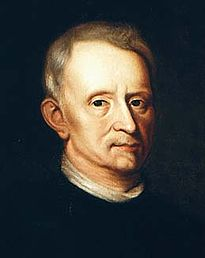
\includegraphics[width=0.5\linewidth]{pictures/gelmont}
%\caption{Я.Б. Ван Гельмонт}
%\label{gelmont}
%\end{figure}
%%%%%%%%%%%%%%%%%%%%%%%%%%%%%%%%%%%%%%%%%%%%%%%%%%%%%%%%%%%%%%%%%%%%%%%%%%%%%%%%%%%%%%%%%%%%%%%%%%%%%%%

\paragraph*{1727} г. С. Гейлс (\ris \ref{ris_1} б) установил, что движение воды по растению вызывают корневое давление и транспирация. 

%%%%%%%%%%%%%%%%%%%%%%%%%%%%%%%%%%%%%%%%%%%%%%%%%%%%%%%%%%%%%%%%%%%%%%%%%%%%%%%%%%%%%%%%%%%%%%%%%%%%%%%%%%% 
%\begin{figure}
%  \centering
%       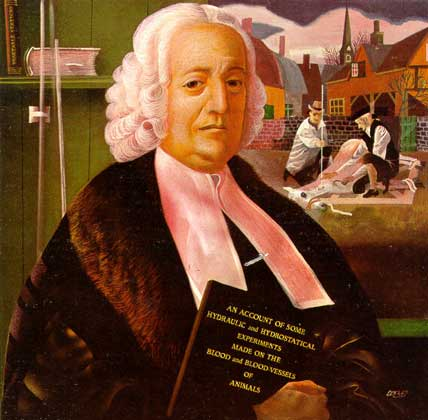
\includegraphics[width=0.5\linewidth]{pictures/geils}
%\caption{С. Гейлс}
%\label{geils}
%\end{figure}
%%%%%%%%%%%%%%%%%%%%%%%%%%%%%%%%%%%%%%%%%%%%%%%%%%%%%%%%%%%%%%%%%%%%%%%%%%%%%%%%%%%%%%%%%%%%%%%%%%%%%%%

\begin{figure}[h]
\begin{minipage}[h]{0.49\linewidth}
\center{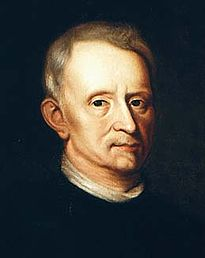
\includegraphics[width=0.7\linewidth]{pictures/gelmont} \\ а) Я.Б. Ван Гельмонт}
\end{minipage}
\hfill
\begin{minipage}[h]{0.49\linewidth}
\center{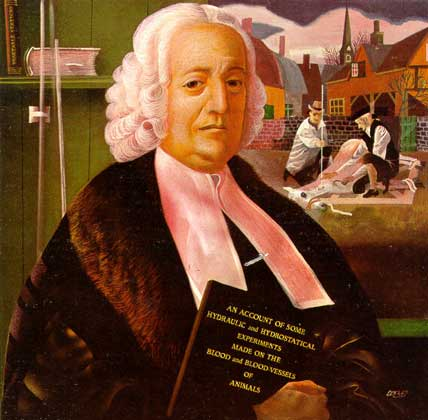
\includegraphics[width=0.9\linewidth]{pictures/geils} \\ б) С. Гейлс}
\end{minipage}
%\caption{Зависимость сигнала от шума для данных.}
\label{ris_1}
\end{figure}

%%%%%%%%%%%%%%%%%%%%%%%%%%%%%%%%%%%%%%%%%%%%%%%%%%%%%%%%%%%%%%%%%%%%%%%%%%%%%%

\paragraph*{1771} г. Дж. Пристли (\ris \ref{ris_2} а) открыл способность зеленых растений выделять на свету кислород.

%%%%%%%%%%%%%%%%%%%%%%%%%%%%%%%%%%%%%%%%%%%%%%%%%%%%%%%%%%%%%%%%%%%%%%%%%%%%%%%%%%%%%%%%%%%%%%%%%%%%%%%%%%% 
%\begin{figure}
%  \centering
%       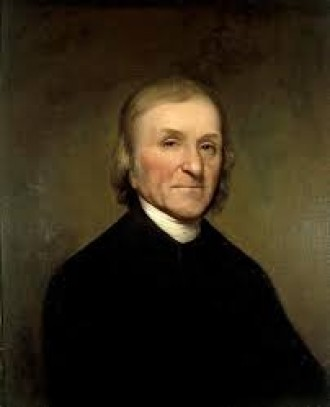
\includegraphics[width=0.5\linewidth]{pictures/pristli}
%\caption{С. Гейлс}
%\label{pristli}
%\end{figure}
%%%%%%%%%%%%%%%%%%%%%%%%%%%%%%%%%%%%%%%%%%%%%%%%%%%%%%%%%%%%%%%%%%%%%%%%%%%%%%%%%%%%%%%%%%%%%%%%%%%%%%% 

\paragraph*{1782} г. Ж. Сенебье (\ris \ref{ris_2} б) назвал поглощение $СО_{2}$ на свету <<углекислотным дыханием>>.  

%%%%%%%%%%%%%%%%%%%%%%%%%%%%%%%%%%%%%%%%%%%%%%%%%%%%%%%%%%%%%%%%%%%%%%%%%%%%%%%%%%%%%%%%%%%%%%%%%%%%%%%%%%% 
%\begin{figure}
%  \centering
%       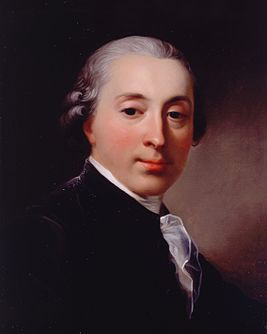
\includegraphics[width=0.5\linewidth]{pictures/senebier}
%\caption{Ж. Сенебье}
%\label{senebier}
%\end{figure}
%%%%%%%%%%%%%%%%%%%%%%%%%%%%%%%%%%%%%%%%%%%%%%%%%%%%%%%%%%%%%%%%%%%%%%%%%%%%%%%%%%%%%%%%%%%%%%%%%%%%%%% 

%%%%%%%%%%%%%%%%%%%%%%%%%%%%%%%%%%%%%%%%%%%%%%%%%%%%%%%%%%%%%%%%%%%%%%%%%%%%%%%%%%%%%%%%%%%%%%%%%%%%%%%

\begin{figure}[h]
\begin{minipage}[h]{0.49\linewidth}
\center{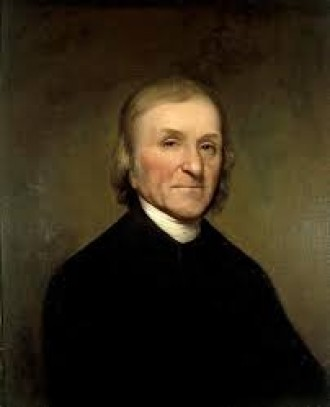
\includegraphics[width=0.8\linewidth]{pictures/pristli} \\ а) Пристли}
\end{minipage}
\hfill
\begin{minipage}[h]{0.49\linewidth}
\center{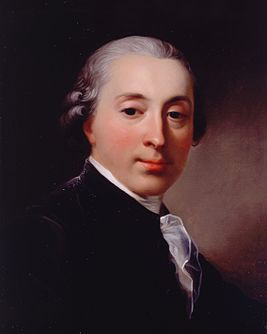
\includegraphics[width=0.8\linewidth]{pictures/senebier} \\ б) Ж. Сенебье}
\end{minipage}
%\caption{Зависимость сигнала от шума для данных.}
\label{ris_2}
\end{figure}

%%%%%%%%%%%%%%%%%%%%%%%%%%%%%%%%%%%%%%%%%%%%%%%%%%%%%%%%%%%%%%%%%%%%%%%%%%%%%%

\paragraph*{1797–1804} гг. Н. Т. Соссюр открыл дыхание у растений и рассчитал баланс газов при фотосинтезе. 

%%%%%%%%%%%%%%%%%%%%%%%%%%%%%%%%%%%%%%%%%%%%%%%%%%%%%%%%%%%%%%%%%%%%%%%%%%%%%%%%%%%%%%%%%%%%%%%%%%%%%%%%%%% 
\begin{figure}
  \centering
       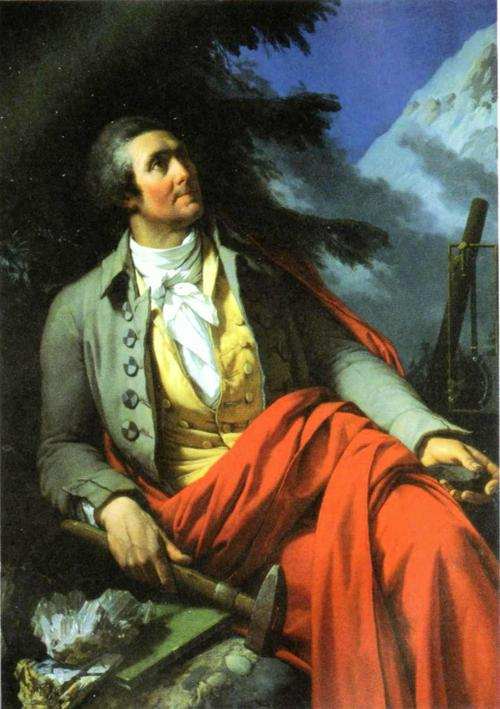
\includegraphics[width=0.35\linewidth]{pictures/saussr}
\caption{Н. Т. Соссюр}
\label{saussr}
\end{figure}
%%%%%%%%%%%%%%%%%%%%%%%%%%%%%%%%%%%%%%%%%%%%%%%%%%%%%%%%%%%%%%%%%%%%%%%%%%%%%%%%%%%%%%%%%%%%%%%%%%%%

\paragraph*{1800} г. Ж. Сенебье опубликовал пятитомный трактат <<Physiologie vegetale>>, в котором впервые определил физиологию растений как самостоятельную науку.

\subsection*{Цель и задачи физиологии растений}


\remember{Согласно современному определению \gls{fzrsc} изучает общие закономерности жизнедеятельности растительных организмов и является частью биологической науки}

\paragraph*{}Задачами физиологии на сегодняшний момент являются:

\begin{enumerate}

	\item изучение закономерностей жизнедеятельности растений (механизмы питания, роста, движения, размножения и др.); 
	\item разработка теоретических основ получения максимальных урожаев сельскохозяйственных культур; 
	\item разработка установок для осуществления процессов фотосинтеза в искусственных условиях.

\end{enumerate}

\paragraph*{}Физиология растений делится на две ветви: общую и прикладную. Задачей прикладной физиологии является изучение конкретных видов растений в конкретных экологических условиях.

\paragraph*{}Физиология растений служит основой для ряда других наук: агрохимии (наука о почвенном питании растений), растениеводства (наука о возделывании отдельных видов растений), селекции (наука о выведении новых сортов растений), фитопатологии (наука об инфекционных заболеваниях растений).

\subsection*{Место зеленого растения в природе и жизни человека}

\paragraph*{}Автотрофные растения Мирового океана за год способны превращать в органическое вещество 20–155 109 т углерода. Наземные растения фиксируют 16–24 109 т углерода. 
Только наземные растения накапливают ежегодно в форме углеводов 5-10 17 ккал. Даже 1 \% этой энергии достаточно для питания 5 млрд. человек. }
	
\chapter{Теоретический раздел}

		\section{Предмет, методы и история развития физиологии растений}
	
	\paragraph*{}\note{Любая наука включает в себя предмет исследований, методы исследований и ученых, которые этими исследованиями занимаются}

\paragraph*{}\gls{fzrsc} -- это наука о процессах, происходящих в растительном организме: почвенное, воздушное и гетеротрофное питание, синтез, транспорт и распад веществ, рост и развитие, движения растений, взаимодействие с патогенами, реакции на неблагоприятные факторы внешней среды. 


\paragraph*{}\gls{fzrsc} занимается процессами, происходящими на разных уровнях организации: молекулярном, субклеточном, клеточном, тканевом, органном, организменном и биоценотическом. Однако надо всегда иметь в виду, что в растении все процессы на любом уровне организации взаимосвязаны. Изменение какого-либо процесса сказывается на всей жизнедеятельности организма.

\subsection*{История развития знаний о физиологии растения}

\paragraph*{}Историю развития физиологии растений как науки можно поделить на три этапа:

\begin{enumerate}
\item Этап первичного накопления знаний;
\item Этап формирования физиологии растений как науки;
\item Современный этап;
\end{enumerate}

\subsubsection*{Этап первичного накопления знаний}

\paragraph*{}\gls{fzrsc} зародилась в XVII—XVIII веках в классических трудах итальянского биолога и врача М. Мальпиги <<Анатомия растений>> и английского ботаника и врача С. Гейлса <<Статика растений>>. Первоначально \gls{fzrsc} являлась частью ботаники и изучала питание растений.

\paragraph*{1634} Я.Б. Ван Гельмонт (\ris \ref{ris_1} а) в своей книге сделан вывод о том, что вода используется для построения органической массы растения.

\note{Выращивая в течение 5 лет ивовую ветвь в горшке со взвешенной почвой, Ван Гельмон установил, что за время опыта вес ветви увеличился в 30 раз, тогда как вес почвы почти не изменился. Гельмонт пришёл к заключению, что основной источник питания растения не почва, а вода. Несмотря на ошибочность такого вывода, этот опыт имел большое значение, т.к. при изучении растений впервые был применен количественный метод -- взвешивание}

%%%%%%%%%%%%%%%%%%%%%%%%%%%%%%%%%%%%%%%%%%%%%%%%%%%%%%%%%%%%%%%%%%%%%%%%%%%%%%%%%%%%%%%%%%%%%%%%%%%%%%%%%%% 
%\begin{figure}
%  \centering
%       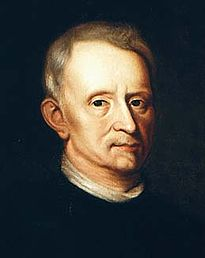
\includegraphics[width=0.5\linewidth]{pictures/gelmont}
%\caption{Я.Б. Ван Гельмонт}
%\label{gelmont}
%\end{figure}
%%%%%%%%%%%%%%%%%%%%%%%%%%%%%%%%%%%%%%%%%%%%%%%%%%%%%%%%%%%%%%%%%%%%%%%%%%%%%%%%%%%%%%%%%%%%%%%%%%%%%%%

\paragraph*{1727} г. С. Гейлс (\ris \ref{ris_1} б) установил, что движение воды по растению вызывают корневое давление и транспирация. 

%%%%%%%%%%%%%%%%%%%%%%%%%%%%%%%%%%%%%%%%%%%%%%%%%%%%%%%%%%%%%%%%%%%%%%%%%%%%%%%%%%%%%%%%%%%%%%%%%%%%%%%%%%% 
%\begin{figure}
%  \centering
%       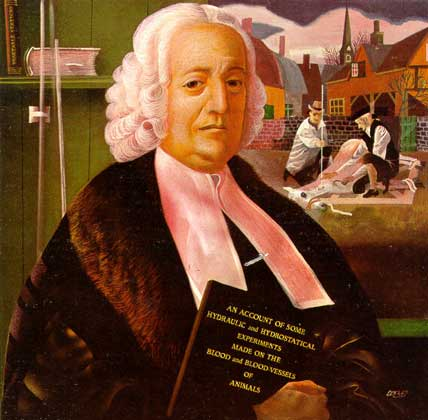
\includegraphics[width=0.5\linewidth]{pictures/geils}
%\caption{С. Гейлс}
%\label{geils}
%\end{figure}
%%%%%%%%%%%%%%%%%%%%%%%%%%%%%%%%%%%%%%%%%%%%%%%%%%%%%%%%%%%%%%%%%%%%%%%%%%%%%%%%%%%%%%%%%%%%%%%%%%%%%%%

\begin{figure}[h]
\begin{minipage}[h]{0.49\linewidth}
\center{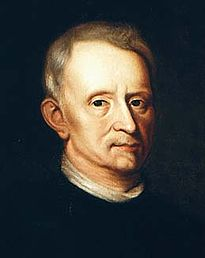
\includegraphics[width=0.7\linewidth]{pictures/gelmont} \\ а) Я.Б. Ван Гельмонт}
\end{minipage}
\hfill
\begin{minipage}[h]{0.49\linewidth}
\center{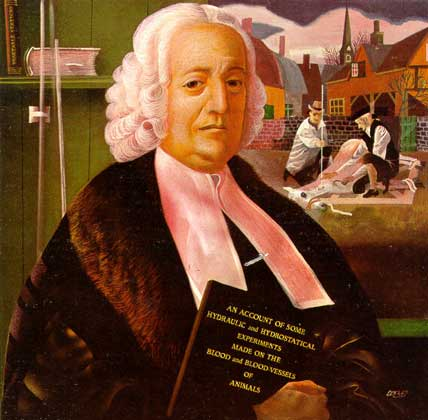
\includegraphics[width=0.9\linewidth]{pictures/geils} \\ б) С. Гейлс}
\end{minipage}
%\caption{Зависимость сигнала от шума для данных.}
\label{ris_1}
\end{figure}

%%%%%%%%%%%%%%%%%%%%%%%%%%%%%%%%%%%%%%%%%%%%%%%%%%%%%%%%%%%%%%%%%%%%%%%%%%%%%%

\paragraph*{1771} г. Дж. Пристли (\ris \ref{ris_2} а) открыл способность зеленых растений выделять на свету кислород.

%%%%%%%%%%%%%%%%%%%%%%%%%%%%%%%%%%%%%%%%%%%%%%%%%%%%%%%%%%%%%%%%%%%%%%%%%%%%%%%%%%%%%%%%%%%%%%%%%%%%%%%%%%% 
%\begin{figure}
%  \centering
%       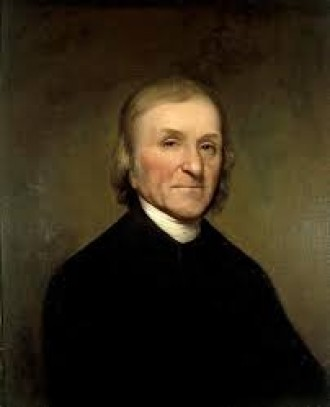
\includegraphics[width=0.5\linewidth]{pictures/pristli}
%\caption{С. Гейлс}
%\label{pristli}
%\end{figure}
%%%%%%%%%%%%%%%%%%%%%%%%%%%%%%%%%%%%%%%%%%%%%%%%%%%%%%%%%%%%%%%%%%%%%%%%%%%%%%%%%%%%%%%%%%%%%%%%%%%%%%% 

\paragraph*{1782} г. Ж. Сенебье (\ris \ref{ris_2} б) назвал поглощение $СО_{2}$ на свету <<углекислотным дыханием>>.  

%%%%%%%%%%%%%%%%%%%%%%%%%%%%%%%%%%%%%%%%%%%%%%%%%%%%%%%%%%%%%%%%%%%%%%%%%%%%%%%%%%%%%%%%%%%%%%%%%%%%%%%%%%% 
%\begin{figure}
%  \centering
%       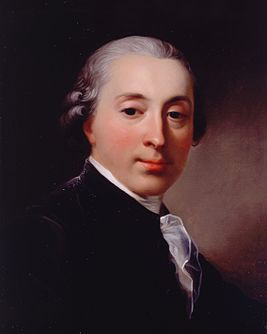
\includegraphics[width=0.5\linewidth]{pictures/senebier}
%\caption{Ж. Сенебье}
%\label{senebier}
%\end{figure}
%%%%%%%%%%%%%%%%%%%%%%%%%%%%%%%%%%%%%%%%%%%%%%%%%%%%%%%%%%%%%%%%%%%%%%%%%%%%%%%%%%%%%%%%%%%%%%%%%%%%%%% 

%%%%%%%%%%%%%%%%%%%%%%%%%%%%%%%%%%%%%%%%%%%%%%%%%%%%%%%%%%%%%%%%%%%%%%%%%%%%%%%%%%%%%%%%%%%%%%%%%%%%%%%

\begin{figure}[h]
\begin{minipage}[h]{0.49\linewidth}
\center{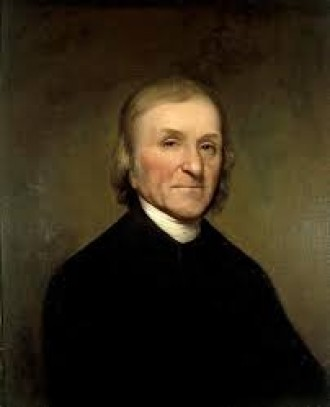
\includegraphics[width=0.8\linewidth]{pictures/pristli} \\ а) Пристли}
\end{minipage}
\hfill
\begin{minipage}[h]{0.49\linewidth}
\center{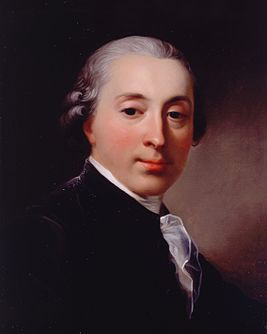
\includegraphics[width=0.8\linewidth]{pictures/senebier} \\ б) Ж. Сенебье}
\end{minipage}
%\caption{Зависимость сигнала от шума для данных.}
\label{ris_2}
\end{figure}

%%%%%%%%%%%%%%%%%%%%%%%%%%%%%%%%%%%%%%%%%%%%%%%%%%%%%%%%%%%%%%%%%%%%%%%%%%%%%%

\paragraph*{1797–1804} гг. Н. Т. Соссюр открыл дыхание у растений и рассчитал баланс газов при фотосинтезе. 

%%%%%%%%%%%%%%%%%%%%%%%%%%%%%%%%%%%%%%%%%%%%%%%%%%%%%%%%%%%%%%%%%%%%%%%%%%%%%%%%%%%%%%%%%%%%%%%%%%%%%%%%%%% 
\begin{figure}
  \centering
       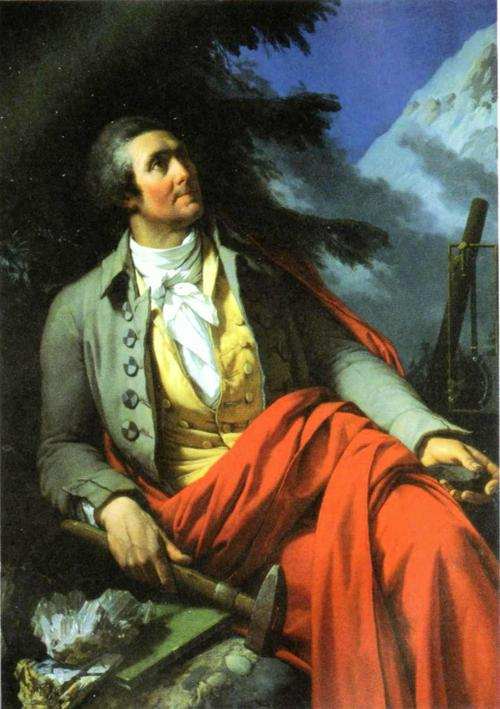
\includegraphics[width=0.35\linewidth]{pictures/saussr}
\caption{Н. Т. Соссюр}
\label{saussr}
\end{figure}
%%%%%%%%%%%%%%%%%%%%%%%%%%%%%%%%%%%%%%%%%%%%%%%%%%%%%%%%%%%%%%%%%%%%%%%%%%%%%%%%%%%%%%%%%%%%%%%%%%%%

\subsubsection*{Этап формирования физиологии растений как науки}

\paragraph*{1800} г. Ж. Сенебье опубликовал пятитомный трактат <<Physiologie vegetale>>, в котором впервые определил физиологию растений как самостоятельную науку.

\paragraph*{1896} Русский биохимик А.Н. Бах создал перекисную теорию биологического окисления, являющуюся фундаментом современной теории радикалов.

\paragraph*{}Немецкий биохимик О. Варбург открыл роль железа как структурного элемента ферментов, связанных с биологическим окислением. 

\paragraph*{}Английский учёный Д. Кейлин открыл \gls{cytochrom}ы – важнейшую группу соединений, участвующих в транспорте электронов как в фотосинтезе, так и в дыхании.

\subsection*{Цель и задачи физиологии растений}


\remember{Согласно современному определению \gls{fzrsc} изучает общие закономерности жизнедеятельности растительных организмов и является частью биологической науки}

\paragraph*{}Задачами физиологии на сегодняшний момент являются:

\begin{enumerate}

	\item Изучение закономерностей жизнедеятельности растений (механизмы питания, роста, движения, размножения и др.); 
	\item Разработка теоретических основ получения максимальных урожаев сельскохозяйственных культур; 
	\item Разработка установок для осуществления процессов фотосинтеза в искусственных условиях.

\end{enumerate}

\paragraph*{}Физиология растений делится на две ветви: общую и прикладную. Задачей прикладной физиологии является изучение конкретных видов растений в конкретных экологических условиях.

\paragraph*{}Физиология растений служит основой для ряда других наук: агрохимии (наука о почвенном питании растений), растениеводства (наука о возделывании отдельных видов растений), селекции (наука о выведении новых сортов растений), фитопатологии (наука об инфекционных заболеваниях растений).

\subsection*{Место зеленого растения в природе и жизни человека}

\paragraph*{}Автотрофные растения Мирового океана за год способны превращать в органическое вещество 20–155*$10^{9}$ т углерода. Наземные растения фиксируют 16–24*$10^{9}$ т углерода. 
Только наземные растения накапливают ежегодно в форме углеводов 5*$10^{17}$ ккал. Даже 1 \% этой энергии достаточно для питания 5 млрд. человек. 

	\section{Структурная и функциональная организация растительной клетки}
	
	%Лекция 1
\paragraph*{}\note{Традиционно, деление живых организмов на царства осуществляется на основе особенностей организации их клетки. Ниже приведены особенности строения клетки растений, которые служат основанием для выделения растений в отдельное царство Planta.}

\paragraph*{}Клетка — основная функциональная часть растительного организма. 
%У растений, в отличии от животных нет систем органов. 

\paragraph*{}Все растения являются многоклеточными организмами, клетки которых дифференцированы согласно выполняемым функциям \footnote{В 70-80 годах растения разделяли на высшие и низшие. В последнюю группу включались ряд одноклеточных организмов, таких как хлорелла и хламидомонада. Однако сейчас все одноклеточные организмы объеденные в царство Простейшие}

\paragraph*{}Строение растительной клетки во многом сходно со сторением клеток животных и грибов: как и у всех \hyperlink{q_prok_cell}{\termin{эукариотических}} организмов, клетки растений имеют в своем составе ядро, цитоплазму, ряд клеточных органелл и систему мембран (\ris \ref{cell_shema}) \footnote{Так как строение клетки и функции ее компонентов подробно рассматриваются на курсе <<Цитология>>, то мы не будем подробно останавливаться на общих чертах растительной клетки а опишем лишь структуры характерные только для клеток растений. Общее же строение клетки можно повторить на основе учебника по физиологии растений, например В.М. Юрина \cite{urin_2010}.}

\paragraph*{}Специфической особенностью строения растительной клетки является:

\begin{enumerate}
    \item наличие прочной полисахаридной \hyperlink{cell_wall}{клеточной стенки}
    \item наличие крупной \hyperlink{cell_vakuol}{центральной вакуоли}
	\item наличие системы \hyperlink{cell_plastids}{пластид}
	
\end{enumerate}

%%%%%%%%%%%%%%%%%%%%%%%%%%%%%%%%%%%%%%%%%%%%%%%%%%%%%%%%%%%%%%%%%%%%%%%%%%%%%%%%%%%%%%%%%%%%%%%%%%%%%%%%%%% 
\begin{figure}
  \centering
       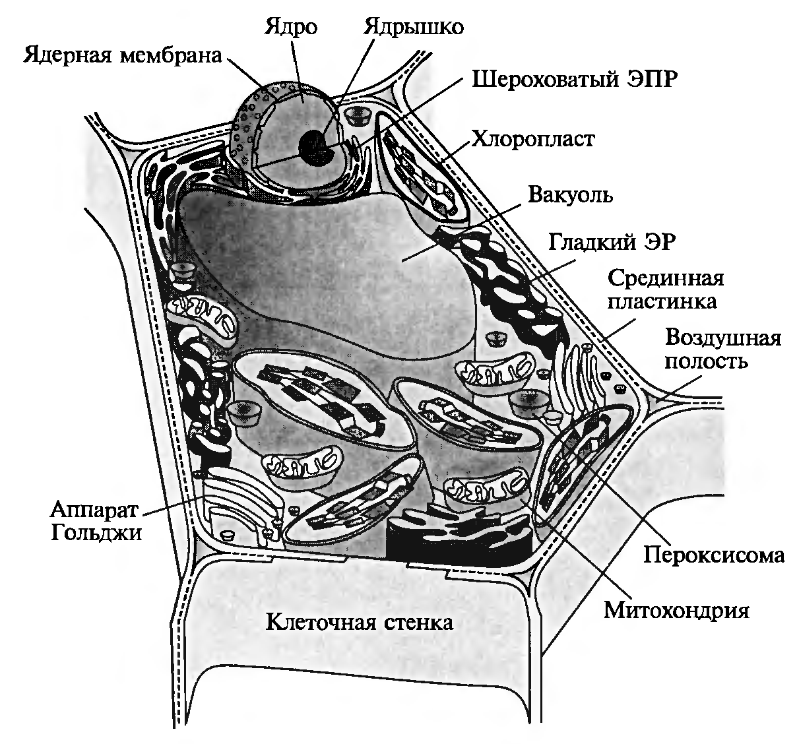
\includegraphics[width=0.5\linewidth]{pictures/plant_cell}
\caption{Строение растительной клетки}
\label{cell_shema}
\end{figure}
%%%%%%%%%%%%%%%%%%%%%%%%%%%%%%%%%%%%%%%%%%%%%%%%%%%%%%%%%%%%%%%%%%%%%%%%%%%%%%%%%%%%%%%%%%%%%%%%%%%%%%%

%\paragraph*{}Растительная клетка содержит три относительно автономные, но тесно взаимодействующие генетические системы: 1. ядерную, 2. митохондриальную и 3. пластидную. Для растительных клеток характерен особый тип роста – рост растяжением. У делящихся растительных клеток отсутствуют центриоли. Клеточные стенки всех клеток контактируют друг с другом, образуя единую систему стенок — апопласт. 

\subsection*{Клеточная стенка}

\paragraph*{}Химический состав и структура \hypertarget{cell_wall}{клеточной стенки} обеспечивают ее важнейшие свойства -- прочность, эластичность и высокую способность впитывать воду -- \termin{гидрофильность}.

\paragraph*{}Основой химического состава клеточной стенки являются полисахариды: \hyperlink{cellulosa}{целлюлоза} -- 25\%, гемицеллюлоза -- 40 \% и пектиновые вещества -- 30 \%. На долю белков и остальных веществ приходится только 5 \% от массы клеточной стенки. 

\paragraph*{}Тонкие нити целлюлозы переплетаются образуя сеть, которая погружена в аморфный \termin{матрикс}.

\paragraph*{}\note{Таким образом, клеточная стенка напоминает по структуре железобетон, где сеть из железных прутьев погружена в слой бетона}

\paragraph*{}В клеточной стенке различают первичную и вторичную оболочки.

\paragraph*{}Первичная оболочка отличается большим количеством гемицеллюлозы и пектина. Она очень гигроскопична. Формирование первичной оболочки заканчивается с окончанием роста клетки.

\paragraph*{}Вторичная оболочка начинает формироваться по окончании роста клетки. Откладывается на внутренней поверхности клеточной стенки. Образованна целлюлозой.

\paragraph*{}Между первичными оболочками соседних клеток находится прослойка пектина -- \termin{серединная пластинка}. При разрушении срединной пластинки (\termin{мацерации}) клетки разъединяются.

\paragraph{Функции клеточной стенки}

\begin{enumerate}

	\item Опорная-- КС придает постоянную форму растительным клеткам, и растения в целом \footnote{На прочности клеточной стенки основано функционирование механических тканей растения - колленхимы и склеренхимы}
	\item Защитная -- КС защищает клетку от разрушения гидростатическим давлением и от проникновения инфекций.
	\item Принимает участие в поглощении минеральных веществ.

\end{enumerate}

\paragraph*{}Клеточная стенка пронизана порами \termin{\hypertarget{plasmodesma}{плазмодесмами}}, благодаря которым цитоплазма всех клеток объединена в единое целое -- \termin{симпласт}. Через плазмодесмы осуществляется транспорт воды, минеральных веществ и гормонов.


\paragraph*{}Каждая плазмодесма представляет собой тяж \termin{гиалоплазмы}, окруженный плазмалеммой, центральную часть которого занимает \termin{десмотрубка}, которая связывает эндоплазматический ретикулум соседних клеток. Непрерывную систему эндоплазматического ретикулума растения называют эндопластом.

%\paragraph*{}Клеточная стенка. Состоит из целлюлозы, гемицелюлозы и пектиновых веществ, липиды и небольшое количество белков. В стареющих клетках оболочки пропитываются лигнином и суберином. Кроме того, в оболочках растительных клеток найдены ферменты.

\subsection*{Цитоплазматическая мембрана и протопласт}

\paragraph*{}\hypertarget{plasmolema}{Клеточная мембрана} или \termin{плазмолема}, находится под клеточной стенкой. Основу мембраны составляет двойной слой \hyperlink{plipids}{фосфолипидов}. Важной составляющей частью плазмолемы являются так же белки и гликолипиды. 

\paragraph*{}Белки, входящие в состав цитоплазматической мембраны делятся на две группы

\begin{enumerate}
	\item Переферийные белки -- гидрофильные белки, которые возможно легко отделить от мембраны
	\item Интегральные -- гидрофобные белки, прочно связанные с мембраной \cite{fzr_ermakov}
\end{enumerate}

\paragraph*{}Функции мембранных белков

\begin{enumerate}

	\item \hyperlink{enzimes}{ферменты} катализируют ассоциированные с мембраной реакции. 
	\item структурные белки, не имеют ферментативной активности, образуют мембраны
	\item транспортные белки, переносят вещества через мембраны,
	\item белки-рецепторы, воспринимают раздражения,
	\item обеспечивают связь плазмалеммы с цитоскелетом.

\end{enumerate}

\paragraph{Функции плазмолемы}

\begin{enumerate}
	\item Транспортная -- избирательно пропускает вещества из и внутрь клетки.
	\item Осмотическая -- поддерживает осмотические свойства клетки.
	\item Регуляторная -- регулируют обмен веществ (транспорт веществ, активность ферментов);
	\item Структурная -- делят клетку на компартменты (замкнутые полости), имеющие разный химический состав; благодаря мембранам в клетке возникают разные градиенты (химического состава, концентрации, электрические, вязкости);
\end{enumerate}

\remember{\textbf{Избирательная проницаемость} -- это ключевое свойство всех биологических мембран, лежащие в основе способности клетки к поддержанию постоянства состава внутренней среды}

\paragraph*{}\hypertarget{protoplast}{Протопласт} -- живое содержимое клетки. Протопласт состоит из \hypertarget{citoplasma}{цитоплазмы} и органелл: ядра, митохондрий, аппарата Гольджи, рибосом и др., погруженных в матрикс цитоплазмы — гиалоплазму.

\paragraph*{}По химическому составу цитоплазма на 80\% состоит из воды, а на 20\% из сухого вещества -- белков и небольшого количества липидов.

\paragraph*{}Ядро: основная органелла клетки, где сосредоточена большая часть наследственной информации. В молодой клетки -- в центре, потом смещается центральной вакуолью на периферию клетки. Оболочка ядра двойная с порами. Цитоплазма ядра \termin{кариоплазма} содержит деспирализованые хромосомы -- \termin{хроматин}, одно или несколько ядрышек.

\paragraph*{}Функция ядра -- хранение и передача наследственной информации.

\paragraph*{}\hypertarget{mitohondria}{Митохондрии} -- тела палочковидной формы, число митохондрий зависит от физиологического состояния клетки (десятки или тысячи). Имеют сложную структуру: двойная мембрана образует впячивания кристы, на поверхности которых ферменты дыхательной цепи.

\paragraph*{}\note{В отличии от клеток животных, содержащих, как правило, одну большую разветвленную митохондрию, клетки растений содержать множество мелких митохондрий}%Надо проверить и указать литературу

\paragraph*{}Функция митохондрий — участие в аэробном этапе дыхания.

\paragraph*{}\hypertarget{sect_rybosoms}{Рибосомы} -- немембранные органелы, которые состоят из двух субъединиц (большей и малой) и представляют собой сложный комплекс из \hyperlink{proteins}{белков} и \gls{rna}. Функция рибосом -- участие в синтезе белка на этапе трансляции.

\paragraph*{}Комплекс Гольджи представляет собой стопу одномембранных цистерн -- \termin{диктиосом}. Количество таких цистерн может быть различно в зависимости от типа и стадии развития клетки.

\paragraph*{}\note{Например в клетках апикальной меристемы иван-чая содержится примерно 20 единиц, а в клетках хлопка, которые продуцируют волокна -- более 1000 \cite{fzr_ermakov}.} 

\paragraph*{}В отличии от животной клетки, где КГ локализован в центре клетки, в растительной клетки диктиосомы комплекса Гольжджи рассеяны по всей цитоплазме. Кроме того КГ в клетки растения остается целостным и активным в течении \termin{\hyperlink{q_mitos}{митоза}}, чтобы обеспечить синтез клеточной стенки  \cite{fzr_ermakov}.

\paragraph*{}Эндоплазматический ретикулум — система каналов образованных одной мембраной, пронизывающих цитоплазму, связанных с ядром и ретикулумом других клеток через плазмодемсмы. Функции -- участие в синтезе белка, транспорт веществ, разделение клетки на отсеки

\subsection*{Центральная вакуоль}

\paragraph*{}\hypertarget{cell_vakuol}{Центральная вакуоль} это одномембранная органелла характерна только для растительных клеток. Мембрана центральной вакуоли носит название \gls{tonoplast}. В ходе \hyperlink{ontogenesis}{онтогенеза} растительной клетки центральная вакуоль формируется из мелких протовакуолей. У зрелой клетки центральная вакуоль занимает большую часть объема.

\paragraph*{}Функции центральной вакуоли 

\begin{enumerate}
	\item Увеличение площади поверхности клетки \note{Для растений, как для фототрофных организмов, важна большая площадь поверхности клеток, позволяющая разместить большее количество хлоропластов. Центральная вакуоль позволяет увеличить размер, а следовательно и площадь поверхности клетки не за счет структурированной богатой азотом цитоплазмы, а за счет большей вакуоли, наполненной <<дешевым для производство>> соком \cite{fzr_ermakov}}
	\item Создание и поддержание тургорного давления
	\item Регуляция pH --вакуоль служит резервуаром для протонов
	\item Защитная --в вакуоли содержится ряд веществ, защищающих растения от поедания насекомыми и млекопитающими. Среди данных веществ можно выделить токсины (фенольные соединения, алкалоиды), полимеры (каучук, гутта), ферменты
	\item Участие в придании растению окраски -- вакуоли могут содержать водорастворимые пигменты (антоцианы и беталаины) 
	\item Запасание питательных веществ
	\item Запасание вредных для клетки веществ -- внутри вакуолей растения утилизируют токсины и тяжелые металлы в виде оксалатов (\ris \ref{crystals}) и избавляются от них в результате листопада.
\end{enumerate}

%%%%%%%%%%%%%%%%%%%%%%%%%%%%%%%%%%%%%%%%%%%%%%%%%%%%%%%%%%%%%%%%%%%%%%%%%%%%%%%%%%%%%%%%%%%%%%%%%%%%%%%%%%% 
\begin{figure}
  \centering
       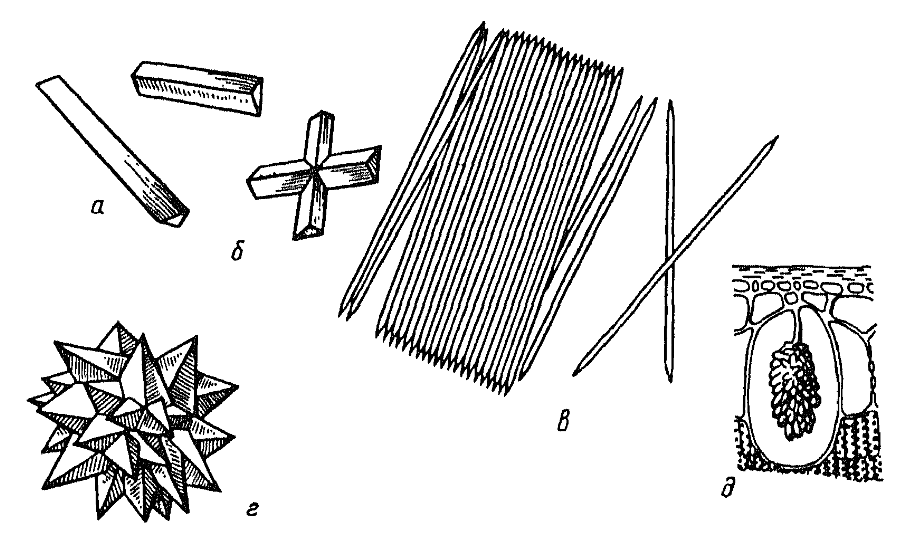
\includegraphics[width=0.5\linewidth]{pictures/crystals}
\caption{Различные типы включений из вакуолей растительной клетки (согласна И.И. Андреевой \cite{andreeva-bot})}
\label{crystals}
\end{figure}
%%%%%%%%%%%%%%%%%%%%%%%%%%%%%%%%%%%%%%%%%%%%%%%%%%%%%%%%%%%%%%%%%%%%%%%%%%%%%%%%%%%%%%%%%% 

\subsection*{Пластиды}

\paragraph*{}\hypertarget{cell_plastids}{Пластиды} делятся на: 

\begin{enumerate}

	\item Хлоропласты 
	\item Хоромопласты 
	\item Лейкопласты (\ris \ref{plastids}). 
	\item Этиопласты

\end{enumerate}



%%%%%%%%%%%%%%%%%%%%%%%%%%%%%%%%%%%%%%%%%%%%%%%%%%%%%%%%%%%%%%%%%%%%%%%%%%%%%%%%%%%%%%%%%%%%%%%%%%%%%%%%%%% 
\begin{figure}
  \centering
       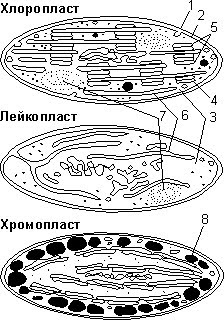
\includegraphics[width=0.3\linewidth]{pictures/plastids}
\caption{Различные типы пластид}
\label{plastids}
\end{figure}
%%%%%%%%%%%%%%%%%%%%%%%%%%%%%%%%%%%%%%%%%%%%%%%%%%%%%%%%%%%%%%%%%%%%%%%%%%%%%%%%%%%%%%%%%% 

\subsubsection*{Хлоропласты}

\paragraph*{}\hyperlink{question_hloroplast}{Хлоропласты} -- двумембранные органоиды линзообразной формы и размером 4-10 мкм. Внутренняя мембрана хлоропласта образует многочисленные впячивания -- \termin{тилакоиды}, служащие для увеличения ее поверхности. Стопка, образованная внутренними мембранами -- тилакоидами называется \termin{грана}. Соседние граны связаны одиночными мембранами-тилакоидами, носящими название \termin{ламеллы}. На мембранах тилакоидов находятся пигменты (хлорофиллы) и белки, принимающие участие в фотосинтеза.

\paragraph*{}Внутри хлоропласта есть своя цитоплазма -- \termin{матрикс}, свои рибосомы. Хлоропласты имеют кольцевую ДНК и все необходимые для синтеза \hyperlink{proteins}{белка} компоненты. Геном хлоропластов кодирует лишь часть необходимых белков; другую часть кодирует ядерный геном фотосинтезирующей клетки. 

\paragraph*{}Хлоропласты возникают \textit{de novo} из инициальных частиц, а также могут размножаться путем простого деления.

\paragraph*{}В растениях хлоропласты локализуются в основном клетках листьев и молодых стеблей. Число хлоропластов обычно составляет от 20 до 100 на клетку. Хлоропласты содержат следующие типы пигментов:

\begin{enumerate}

\item хлорофиллы А и B
\item каротиноиды (оранжевый каротин и желтый ксантофилл)

\end{enumerate}

\paragraph*{}Основная функция хлоропластов -- фотосинтез \footnote{Более подробно строение и функции хлоропластов будут рассмотрены в разделе, посвященном фотосинтезу}. Хлоропласты большинства растений способны перемещаться по клетке в зависимости от интенсивности и направления освещения.

\subsubsection*{Остальные пластиды}

\paragraph*{}Хромопласты встречают в клетках лепестков, зрелых плодов, листьев.
Форма хромопластов может быть: 

\begin{enumerate}

	\item дисковидная
	\item шаровидная
	\item палочковидная
	\item веретенообразная

\end{enumerate}

\paragraph*{}Хромопласты содержат красные, оранжевые и желтые пигменты из группы каротиноидов. Функция хромопластов -- привлечение насекомых-опылителей и животных-распространителей семян.

\paragraph*{}Лейкопласты – бесцветные пластиды, шарообразной или веретенообразной формы. 

\paragraph*{}Функция лейкопластов -- запас питательных веществ. 

\note{Особенно много лейкопластов в запасающих органах – корнях, семенах, плодах, молодых листьях и др.}

\paragraph*{}В зависимости от природы накапливающихся веществ лейкопласты делят на:

\begin{enumerate}

	\item амилопласты -- запасаются углеводы (в большинстве случаев)
	\item олеопласты -- запасаются жиры 
	\item протеинопласты -- запасаются белки

\end{enumerate}

\paragraph*{}этиопласты -- пластиды, формирующиеся при недостаточном освещении и не содержащие хлорофиллов

\subsection*{Вопросы и задания для самоконтроля}

\begin{enumerate}
	\item{Повторите строение \hypertarget{q_prok_cell}{прокариотической клетки}. Составьте таблицу, отражающую различия в строении прокариотической и эукариотической клеток.}
	\item На какие стадии подразделяется \hypertarget{q_mitos}{митоз}, чем деление путем митоза отличается от мейотического деления? Данные сведения вы можете повторить по любому учебнику общей биологии.
	\item Сравните строение \hypertarget{question_hloroplast}{хлоропласта} и бактериальной клетки. В чем проявляется сходство между ними, а в чем различия.
\end{enumerate}



	
	\section{Химический состав растительной клетки}
	
	\section*{Химический состав растительной клетки}

\paragraph*{}Все химические вещества, входящие в состав клетки можно условно разделить на две группы:

\begin{enumerate}
	\item Конституционные -- служат для построения различных структур клетки
	\item Запасающие -- синтезируются как запас питательных веществ
\end{enumerate}

\paragraph*{}Массовая доля различных химических, входящих в состав клетки растения следующая:

\begin{itemize}

	\item 85\% вода
	\item 1,5\% другие неорганических веществ
	\item 10\% белки
	\item 1,1\% нуклеиновые кислоты
	\item 2\% липиды
	\item 0,4\% углеводы

\end{itemize}

\subsection*{Минеральные вещества} 

\subsubsection*{Вода}

\paragraph*{}В основном (80-90\%) \hyperlink{question_aqua}{воды} в клетке находится в особой органелле -- \hyperlink{question_vakual_rep}{центральной вакуоли}. 

\remember{Большая часть воды в клетке находится в \textbf{связанном} состоянии}

\paragraph*{}Различают следующие типы связанной воды:

\begin{enumerate}
	\item Осмотически-связанная низкомолекулярными соединений (моносахаридов, ионов и др.). Гидратирует ионы и коллоиды
	\item Коллоидно-связанная высокомолекулярными соединениями (целлюлоза, гемицеллюлоза, пектин, молекулы белка). Поддерживает структуру коллоидов и обеспечивает функционирование ферментов. Малоподвижна -- не участвует в растворении и транспорте веществ.
	\item Капиллярно-связанная -- в капиллярах клеточной стенки
	\item Химически связанная
\end{enumerate}

\paragraph*{}Роль воды в клетке растения:

\begin{enumerate}

   \item Участие в химических реакциях. Вода является средой где протекают химические реакции и непосредственным участником химических реакций. Например реакции фотосинтеза \ref{fotosynteses_example} идут в водной среде матрикса хлоропластов и при участии молекул воды.
   \item Поддержание структуры клеток. Форма клетки поддерживается за счет \termin{тургорного} давления воды. За счет высокого тургорного давления функционирует, например, механическая ткань \termin{колленхима} (\ris \ref{collenhima}).
   \item Транспорт веществ -- как органические так и неорганические вещества перемещаются внутри клетки и всего организма растения в растворенном виде.
   \item Участие в терморегуляции -- благодаря высокой теплоемкости вода способна смягчать воздействие на клетку резкого перепада температур.
   \item Участие в росте клетки -- клетка увеличивается в размерах за счет действия тургорного давления на клеточную стенку.

\end{enumerate}

\begin{equation}
	6H_{2}O + 6CO_{2} = C_{6}H_{12}O_{6} + 6O_{2}
	\label{fotosynteses_example}
\end{equation}

%%%%%%%%%%%%%%%%%%%%%%%%%%%%%%%%%%%%%%%%%%%%%%%%%%%%%%%%%%%%%%%%%%%%%%%%%%%%%%%%%%%%%%%%%%%%%%%%%%%%%%%%%%% 
\begin{figure}
  \centering
       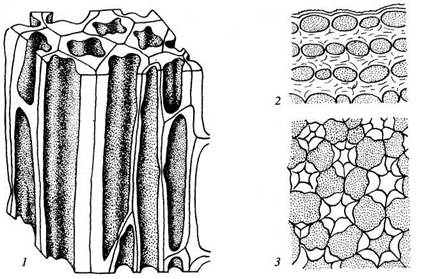
\includegraphics[width=0.5\linewidth]{pictures/collenhima}
\caption{Колленхима}
\label{collenhima}
\end{figure}
%%%%%%%%%%%%%%%%%%%%%%%%%%%%%%%%%%%%%%%%%%%%%%%%%%%%%%%%%%%%%%%%%%%%%%%%%%%%%%%%%%%%%%%%%%

\subsubsection*{Другие неорганические вещества}

\paragraph*{}Неорганические вещества, составляющие в клетке незначительную долю, представлены в основном ионами ($H^{+}$, $K^{+}$, $Na^{+}$, $Ca^{2+}$, $NH_{4}^{+}$ и анионами $OH^{-}$, $SO_{4}^{2+}$, $CO_{3}^{2-}$, $NO_{3}^{-}$, $Cl^{-}$). 

\paragraph*{}Часть от всего запаса неорганических ионов клетки всегда находится в вакуоли в растворенном состоянии и используется клеткой по мере необходимости. 

\paragraph*{}Функции ионов в клетке растения:

\begin{enumerate}
 \item Участие в биохимических процессах -- ионы могут являться элементами ферментов. 
 \item Создание электрического потенциала на мембране клетки
 \item Создание определенного осмотического давления. Осмос лежит в основе процессов поступления воды в растение и ее транспорта. Подробнее этот вопрос будет рассмотрен в разделе, посвященном \hyperlink{whater_circulation}{водному обмену}.
\end{enumerate}

%\paragraph*{}Основная роль ионов: участие в биохимических процессов в качестве составных элементов ферментов, неорганические ионы определяют электрический потенциал клетки участвуют в передаче импульсов возбуждения от клетки к клетке.

%\paragraph*{}Из неорганических веществ растительные клетки (а также, как известно из курса микробиологии, клетки микробов, ведущие фотосинтез и хемосинтез) способны синтезировать органические вещества, которые и определяют накопление биомассы в природы, являясь базовым звеном во всех биоценозах.

\subsection*{Органические вещества}

\paragraph*{}Органические вещества растительной клетки относятся к четырем основным группам\footnote{Так как особенности строения молекул и химические свойства органических веществ изучаются в курсе <<Органическая химия>>, то в данном разделе будет рассмотрена лишь роль различных органических веществ в клетке}

\begin{enumerate}

	\item углеводы
	\item липиды
	\item белки
	\item нуклеиновые кислоты

\end{enumerate}

\subsubsection*{Углеводы: строение, классификация и функции}.

\paragraph*{}\hypertarget{sect_glycosids}{Углеводы} или, сахара являются самыми распространенными в растении органическими веществами. Часть углеводов, например глюкоза, синтезируется в процессе фотосинтеза, другая часть синтезируется в ходе \gls{metabolism}а из других органических веществ. В дальнейшем, в процессе \gls{metabolism}а углеводы участвуют в создании различных органических веществ.

\paragraph*{}Углеводы делятся на 3 группы:

\begin{enumerate}

	\item моносахариды или монозы (простые сахара)
	\item олигосахариды
	\item полисахариды или полиозы

\end{enumerate}

\paragraph*{Моносахариды} -- простые молекулы с числом атомов углерода от 2 до 7. В соответствии с этим она называются: биозы, триозы, тетрозы, пентозы, гексозы, гептозы. Первые три - имеют линейную структуру молекул, последние - циклическую. Общая формула моноз 
$(CH_{2}O)_{n}$. Большинство углеводов в растительной клетке -- пентозы и гексозы.

\paragraph*{}Наиболее известные представители моноз - глюкоза, фруктоза и рибоза (\ris \ref{monogluc}). Монозы легко растворяются в воде, легко вступают в биохимические реакции. 

%%%%%%%%%%%%%%%%%%%%%%%%%%%%%%%%%%%%%%%%%%%%%%%%%%%%%%%%%%%%%%%%%%%%%%%%%%%%%%%%%%%%%%%%%%%%%%%%%%%%%%%

\begin{figure}[h]
\begin{minipage}[h]{0.3\linewidth}
\pyranose{5Sb==CH$_{2}$OH;1Sb==OH;1Sa==H;2Sb==H;2Sa==OH;3Sa==H;3Sb==OH;4Sb==H;4Sa==OH} \\ а) Глюкоза
\end{minipage}
\hfill
\begin{minipage}[h]{0.3\linewidth}
\furanose{4Sb==CH$_{2}$OH;4Sa==H;1Sa==CH$_{2}$OH;1Sb==OH;2Sa==H;2Sb==OH;3Sb==H;3Sa==OH} \\ б) Фруктоза
\end{minipage}
\begin{minipage}[h]{0.3\linewidth}
\furanose{4Sb==CH$_{2}$OH;4Sa==H;1Sa==H;1Sb==OH;2Sa==OH;2Sb==H;3Sb==H;3Sa==OH} \\ в) Рибоза
\end{minipage}
\caption{Моносахариды}
\label{monogluc}
\end{figure}

%%%%%%%%%%%%%%%%%%%%%%%%%%%%%%%%%%%%%%%%%%%%%%%%%%%%%%%%%%%%%%%%%%%%%%%%%%%%%%
\paragraph*{}Одни моносахариды в клетке легко превращаются в другие путем образования и распада фосфорных эфиров (\ris \ref{glucfos})

%%%%%%%%%%%%%%%%%%%%%%%%%%%%%%%%%%%%%%%%%%%%%%%%%%%%%%%%%%%%%%%%%%%%%%%%%%%%%%%%%%%%%%%%%%%%%%%%%%%%%%%%%%% 
\begin{figure}[h!]
  \centering
       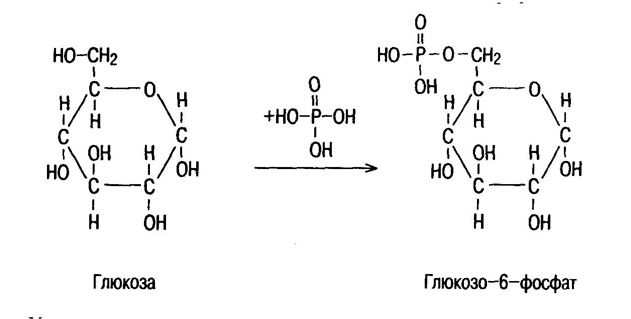
\includegraphics[width=0.5\linewidth]{pictures/glucfos}
\caption{Образование глюкозо фосфата}
\label{glucfos}
\end{figure}
%%%%%%%%%%%%%%%%%%%%%%%%%%%%%%%%%%%%%%%%%%%%%%%%%%%%%%%%%%%%%%%%%%%%%%%%%%%%%%%%%%%%%%%%%% 

\paragraph*{}Как вам известно из курса органической химии, моносахарам свойственна стереоскопическая \hyperlink{question_isomeria_gluc}{изомерия}. При этом в живых организмах сахариды представлены D-изомерами.

%%%%%%%%%%%%%%%%%%%%%%%%%%%%%%%%%%%%%%%%%%%%%%%%%%%%%%%%%%%%%%%%%%%%%%%%%%%%%%%%%%%%%%%%%%%%%%%%%%%%%%%%%%% 
\begin{figure}[h!]
  \centering
       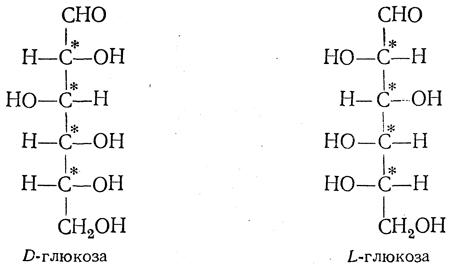
\includegraphics[width=0.5\linewidth]{pictures/dlgluk}
\caption{Моносахариды}
\label{monogluc}
\end{figure}
%%%%%%%%%%%%%%%%%%%%%%%%%%%%%%%%%%%%%%%%%%%%%%%%%%%%%%%%%%%%%%%%%%%%%%%%%%%%%%%%%%%%%%%%%% 

\paragraph*{}Функции моносахаридов:

\begin{enumerate}
	\item Метаболитическая -- глюкоза является субстратом для процессов дыхания и брожения. Глюкоза является исходным веществом для синтеза \hyperlink{krahmal}{крахмала} и \hyperlink{cellulosa}{целлюлозы}. Рибулеза участвует в синтезе углеводов в ходе фотосинтеза, являясь одним из звеньев цикла Кальвина
	\item Структурная -- Рибоза и дезокисрибоза входят в состав нуклеиновых кислот и \gls{atp}
	\item Запасающая -- Глюкоза и фруктоза выступают запасающими веществами в плодах
\end{enumerate}

\paragraph*{Олигосахара} -- это относительно простые молекулы, состоящие всего из 2-3 молекул моноз. В результате гидролиза олигосахаридов образуются моносахара (\ris \ref{hydrolis}).

%%%%%%%%%%%%%%%%%%%%%%%%%%%%%%%%%%%%%%%%%%%%%%%%%%%%%%%%%%%%%%%%%%%%%%%%%%%%%%%%%%%%%%%%%%%%%%%%%%%%%%%%%%% 
\begin{figure}[h!]
  \centering
       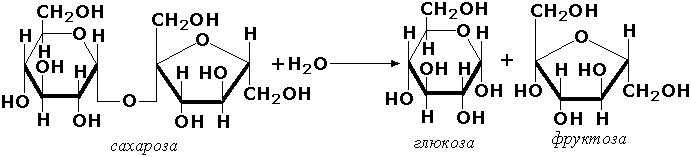
\includegraphics[width=0.5\linewidth]{pictures/hydrolis}
\caption{Гидролиз сахарозы}
\label{hydrolis}
\end{figure}
%%%%%%%%%%%%%%%%%%%%%%%%%%%%%%%%%%%%%%%%%%%%%%%%%%%%%%%%%%%%%%%%%%%%%%%%%%%%%%%%%%%%%%%%%%

\paragraph*{}Наиболее известный представитель олигосахаридов - сахароза. Олигосахариды легко растворяются в воде, участвуют в реакциях синтеза более сложных сахаров.

\paragraph*{}Функции олигосахаридов 

\begin{enumerate}
	\item Запасающая -- сахароза выступает запасающим веществом в корнеплодах свеклы, луковицах лука \cite{zauralov_1995}
	\item Транспортная -- углеводы перемещаются по организму растения в основном в виде сахарозы
\end{enumerate}

\paragraph*{Полисахариды} -- \termin{полимеры}, т.е. сложные молекулы, мономерами которых являются моносахара. Полисахариды нерастворимы в воде и обладают сложной структурой.

\paragraph*{}Наиболее известные представители полисахаридов: \hypertarget{krahmal}{крахмал}, гликоген, \hypertarget{cellulosa}{целлюлоза}, пектины.

\paragraph*{}Крахмал -- это полимер образованный $\alpha$-D глюкозой (\ris \ref{krahmal_mol}).  	

%%%%%%%%%%%%%%%%%%%%%%%%%%%%%%%%%%%%%%%%%%%%%%%%%%%%%%%%%%%%%%%%%%%%%%%%%%%%%%%%%%%%%%%%%%%%%%%%%%%%%%%%%%% 
\begin{figure}[h!]
  \centering
       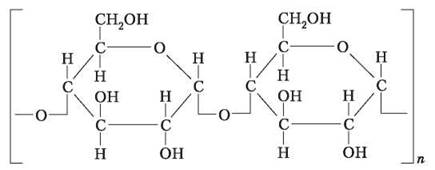
\includegraphics[width=0.5\linewidth]{pictures/krahmal_mol}
\caption{Структура молекулы крахмала}
\label{krahmal_mol}
\end{figure}
%%%%%%%%%%%%%%%%%%%%%%%%%%%%%%%%%%%%%%%%%%%%%%%%%%%%%%%%%%%%%%%%%%%%%%%%%%%%%%%%%%%%%%%%%%

\paragraph*{}Крахмал -- смесь двух гомополисахаридов: линейного -- \termin{амилозы} и разветвленного -- \termin{амилопектина}, общая формула которых $(С_{6}Н_{10}О_{5})_{n}$. Как правило, содержание амилозы в крахмале составляет 10–30\%, амилопектина – 70–90\%. Крахмал имеет молекулярную массу $10^{5}–10^{7}$ \gls{dalton}

\paragraph*{}При действии ферментов или нагревании с кислотами подвергается гидролизу. 

\paragraph*{}Целлюлоза -- это полимер образованный $\beta$-D глюкозой (\ris \ref{cell_mol}).

%%%%%%%%%%%%%%%%%%%%%%%%%%%%%%%%%%%%%%%%%%%%%%%%%%%%%%%%%%%%%%%%%%%%%%%%%%%%%%%%%%%%%%%%%%%%%%%%%%%%%%%%%%% 
\begin{figure}[h!]
  \centering
       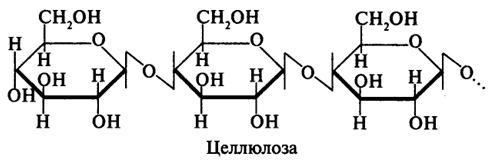
\includegraphics[width=0.5\linewidth]{pictures/cell_mol}
\caption{Структура молекулы целлюлозы}
\label{cell_mol}
\end{figure}
%%%%%%%%%%%%%%%%%%%%%%%%%%%%%%%%%%%%%%%%%%%%%%%%%%%%%%%%%%%%%%%%%%%%%%%%%%%%%%%%%%%%%%%%%%

\paragraph*{}При частичном гидролизе целлюлозы образуется дисахарид \termin{целлобиоза}, а при полном гидролизе – D-глюкоза. Молекулярная масса целлюлозы 1000–2000 кДа. 

\paragraph*{}Инулин – полисахарид, содержащийся в клубнях и корнях георгинов, артишоков и одуванчиков. При его гидролизе образуется фруктоза.

\paragraph*{}Функции Полисахаридов:

\begin{enumerate}

	\item Энергетическая -- при гидролизе полисахаридов образуется глюкоза или фруктоза которые затем могут использоваться растениями в ходе метаболизма.
	\item Строительная -- Целлюлоза и пектин входят в состав \hyperlink{cell_wall}{клеточной стенки}
	\item Запасающая -- крахмал является основным запасным питательным веществом в растении. Главным образом накапливается в семенах (зерна злаков содержат до 70\% крахмала), а также в луковицах, клубнях и сердцевине стебля растений (до 30\%). В небольших количествах он содержится в листьях.

\end{enumerate}

\remember{Крахмал является основным запасным питательным веществом в растении}

\subsubsection*{Липиды: строение, классификация и функции}

\paragraph*{}\hypertarget{sect_lipids}{Липиды} представляют собой достаточно сложные по химической структуре вещества. В их состав также входят углерод, кислород, водород, но в отдельные группы липидов могут входить фосфор, сера, и азот (фосфатиды, пигменты). Все липиды гидрофобны. Функции липидов различны в зависимости от химического строения. Липиды не являются биополимерами.

\remember{Так как жиры не растворимы в воде, они не способны передвигаться по растению. Жиры синтезируются в митохондриях и остаются там до момента использования}

\paragraph*{}Липиды классифицируются на 5 больших групп по признаку функции и сложности строения:

\begin{enumerate}

	\item Жиры
	\item Воска
	\item Фосфатиды
	\item Пигменты
	\item Стероиды
	
\end{enumerate}

\paragraph*{Жиры} или это эфиры состоящие из глицерина и жирных кислот

\paragraph*{}\hyperlink{question_lipid}{Твердые жиры} содержат насыщенные жирные кислоты, например \termin{пальмитиновую} и \termin{стеариновую} называют <<жирами>>, а жидкие жиры с ненасыщенными жирными кислотами, например \termin{олеиновую}, \termin{линолиевую} - <<маслами>>. Твердые жиры - в основном животного происхождения, и масла - растительного, исключения из правила рыбий жир и арахисовое масло \footnote{Насыщенность жира ненасыщенными жирными кислотами определяют по йодному числу (т.е. по количеству граммов йода, связывающегося 100 г жира).}. 

\paragraph*{}Основные функции жиров:

\begin{enumerate}

	\item Энергетическая -- жиры могут служить субстратом для дыхания
	\item Строительная -- фосфолипиды входят в состав \hyperlink{plasmolema}{цитоплазматической мембраны}
	\item Запасающая -- жиры содержатся в плодах и семянах в качестве запасного питательного вещества
	\item Защитная -- накапливаются в зимней период в коре у некоторых древесных растений \cite{zauralov_1995}
\end{enumerate}

\paragraph*{Воска} -- это жироподобные вещества, твердые при комнатной температуре. По химической структуре это сложные эфиры жирных кислот и высокомолекулярных одноатомных спиртов жирного ряда.

\paragraph*{}Основная функция восков - защитная.

\paragraph*{}Фосфатиды, к которым относятся \termin{глицерофосфатиды}, \termin{лецитины} и \termin{кефалины} - это молекулы сложных эфиров глицерина, жирных кислот и фосфорной кислоты. Эти вещества входят в состав запасных жиров и предохраняют их от прогоркания.

\paragraph*{}Кроме того \hypertarget{plipids}{фосфолипиды} входят в состав \hyperlink{plasmolema}{цитоплазматической мембраны}. Сочетание в молекуле фосфолипида остатка фосфорной кислоты и остатков жирных кислот делает молекулу липида полярной -- остаток фосфорной кислоты образует гидрофильную <<головку>>, а остатки жирных кислот -- гидрофобные <<хвосты>>. Благодаря этому в воде молекулы фосфолипидов образуют липидные капли, в которых гидрофильные <<головки>> обращены наружу -- в сторону воды, а гидрофобные <<хвосты>> вовнутрь.

\paragraph*{Пигменты} -- это особая группа липидов, имеющая сложное строение, куда входят и азотистые радикалы. К пигментам относят две группы веществ: хлорофиллы и каротиноиды.

\paragraph*{}Основная функция пигментов - участие в энергетической (световой) фазе фотосинтеза.

\paragraph*{Стероиды и терпены} -- это производные сложного гетероциклического соединения — циклопентанпергидрофенантрена.  В эту группу соединений входят высокомолекулярные спирты стеролы и их сложные эфиры (стериды).

\paragraph*{}Терпены обуславливают аромат эфирных масел растений. К этому классу веществ относится ментол и камфора

%(ну как язык, еще на месте, не сломался).
\paragraph*{}Основная функция стероидов - строительная -- они входят в состав мембран

\subsubsection*{Аминокислоты: строение, классификация и функции}

%\paragraph*{}Аминокислоты - это мономеры белков

\paragraph*{}\hypertarget{aminoacids}{Аминокислоты}, это химические соединения, в состав которых входит одновременно аминогруппа и карбоксильная группа. Кроме того. в состав аминокислот может так же входить сера.

%\paragraph*{}В природе имеется всего 20 аминокислот, из которых затем в живых организмах синтезируется огромное количество белков.

\paragraph*{}Главная функция аминокислот -- строительная. Аминокислоты являются мономерами из которых построена молекула \hyperlink{proteins}{белка}. Причем в состав белковой молекулы могут входить только $\alpha$-аминокислоты.

\paragraph*{}Все аминокислоты классифицируются на 4 группы:

\begin{enumerate}

	\item моноаминомонокарбоновые (глицин, аланин, цистеин, метионин, валин),
	\item моноаминодикарбоновые (аспарагиновая кислота, глутаминовая кислота),
	\item диаминомонокарбоновые (лизин, аргинин),
	\item гетероциклические (триптофан, гистидин).

\end{enumerate}


\paragraph*{}Аминокислоты обладают \hyperlink{aminoacids}{амфотерными свойствами}, способны к образованию между собой особого типа химической связи -- \hypertarget{pept_bound}{\termin{пептидной}} и \termin{дисульфидной} (\ris \ref{dipeptid}) Последовательность из остатков аминокислот, соединенных пептидной связью образуют первичную структуру белковой молекулы.

%%%%%%%%%%%%%%%%%%%%%%%%%%%%%%%%%%%%%%%%%%%%%%%%%%%%%%%%%%%%%%%%%%%%%%%%%%%%%%%%%%%%%%%%%%%%%%%%%%%%%%%%%%% 
\begin{figure}[h!]
  \centering
       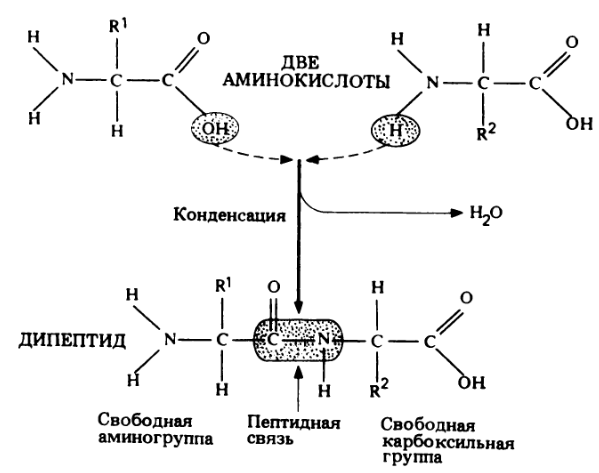
\includegraphics[width=0.5\linewidth]{pictures/dipeptid}
\caption{Схема образования пептидной связи}
\paragraph*{}Согласно Грину \cite{green_bio}
\label{dipeptid}
\end{figure}
%%%%%%%%%%%%%%%%%%%%%%%%%%%%%%%%%%%%%%%%%%%%%%%%%%%%%%%%%%%%%%%%%%%%%%%%%%%%%%%%%%%%%%%%%% 


\remember{В настоящие время в клетках растений обнаружено более 170 видов аминокислот, при этом в состав белка могут входить только 20 видов \cite{green_bio}}

\subsubsection*{Витамины: строение, классификация и функции}

\paragraph*{}\hypertarget{vitamines}{\gls{vitamines}} -- это низкомолекулярные физиологически активные органические соединения различного химического состава. В растениях синтезируются все витамины, а провитамины, которые используют затем животные для создания витаминов животного происхождения, имеют растительное происхождение (например провитамин А и витамин Д).

\paragraph*{}Витамины классифицируются на:

\begin{enumerate}

	\item водорастворимые (С, В, РР, Н, пантотеновая кислота, инозит, фолиевая кислота, пара-аминобензойная кислота),
	\item жирорастворимые (А, Д, Е, К).

\end{enumerate}

\paragraph*{}Для растений особенно важны витамины группы В,РР -- тиамин, ниацин, пиридоксин. Особенно нуждаются в притоке витаминов от фотосинтезирующих органов нефотосинтезирующие органы растения (корни, цветки, плоды).

\paragraph*{}Функция витаминов - участие в биохимических процессах в составе ферментов.

\begin{itemize}

	\item Провитамин A — \termin{каротин} (\ris \ref{vitamins}) наряду с хлорофиллом участвует в поглощении энергии света. Кроме того, он предохраняет хлорофилл от разрушения;
	\item Витамина $B_{1}$ или \termin{тиамин} (\ris \ref{vitamins}) входит в состав фермента отщепляющего углекислоту от пировиноградной кислоты и присоединяющего к этой кислоте углекислого газа;
	\item Витамин $B_{2}$ \termin{рибофлавин} (\ris \ref{vitamins}) способен соединятся с более чем 20-ю различными белками, образуя различные типы ферментов, например карбоксилазу — фермент, необходимый для превращений углеводов;
	\item Витамин C или \termin{аскорбиновая кислота} (\ris \ref{vitamins}) защищает хлорофилл от окисления. Совместно с витамином K участвует в сложных синтетических реакциях, происходящих при фотосинтезе;
	\item Витамины PP или \termin{никатиновая кислота} (\ris \ref{vitamins}), \termin{фолиевая кислота}, \termin{биотин}, \termin{пантотеновая кислота}, входя в состав ферментов, принимающих участие в процессе дыхания, в превращениях азотистых веществ, серы;

\end{itemize}

%%%%%%%%%%%%%%%%%%%%%%%%%%%%%%%%%%%%%%%%%%%%%%%%%%%%%%%%%%%%%%%%%%%%%%%%%%%%%%%%%%%%%%%%%%%%%%%%%%%%%%%%%%% 
\begin{figure}[h!]
  \centering
       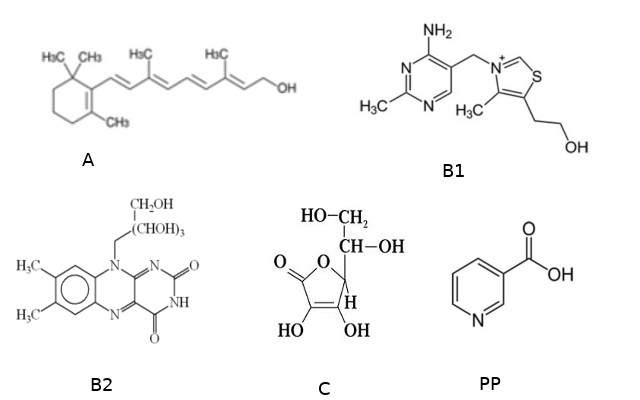
\includegraphics[width=1\linewidth]{pictures/vitamins}
\caption{Формулы некоторых витаминов}
\paragraph*{}Согласно Грину \cite{green_bio}
\label{vitamins}
\end{figure}
%%%%%%%%%%%%%%%%%%%%%%%%%%%%%%%%%%%%%%%%%%%%%%%%%%%%%%%%%%%%%%%%%%%%%%%%%%%%%%%%%%%%%%%%%%

%\subsection*{Белки и нуклеиновые кислоты}

\subsubsection*{Белки: строение, классификация и функции} 

\paragraph*{}\hypertarget{proteins}{Белки} -- это сложные биополимеры, мономером которых являются \hyperlink{aminoacids}{аминокислоты}. Доля белков в растении гораздо меньше, чем в животном организме.  

\paragraph*{}Молекула белка -- это довольно сложна, и в ее структуре можно выделить 3-4 уровня организации (\ris \ref{proteins_struct}).

%%%%%%%%%%%%%%%%%%%%%%%%%%%%%%%%%%%%%%%%%%%%%%%%%%%%%%%%%%%%%%%%%%%%%%%%%%%%%%%%%%%%%%%%%%%%%%%%%%%%%%%%%%% 
\begin{figure}[h!]
  \centering
       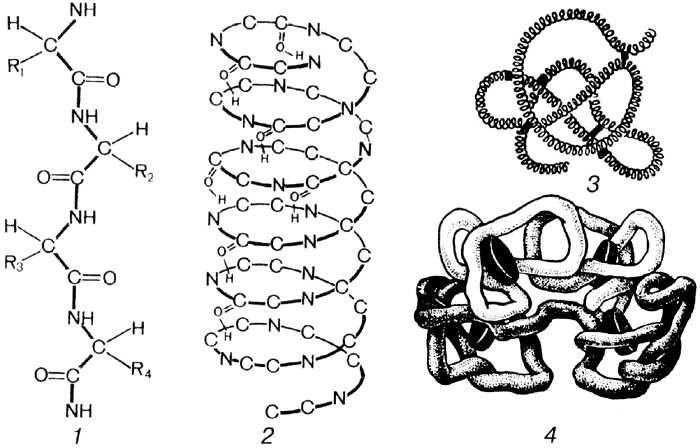
\includegraphics[width=0.7\linewidth]{pictures/proteins_struct}
\caption{Уровни организации белковой молекулы}

\label{proteins_struct}
\end{figure}
%%%%%%%%%%%%%%%%%%%%%%%%%%%%%%%%%%%%%%%%%%%%%%%%%%%%%%%%%%%%%%%%%%%%%%%%%%%%%%%%%%%%%%%%%%

\paragraph*{}При этом пространственная структура молекулы поддерживается меж- и внутримолекулярными взаимодействиями следующих типов:

\begin{enumerate}

	\item \hyperlink{pept_bound}{Пептидные связи} -- участвуют в образовании полипептидной цепочки белковой молекулы. Последовательность аминокислот в полипептидной цепочке -- это первичная структура белка.
	\item \hyperlink{question_chem_bounds}{Нековалентные водородные} связи между соседними аминокислотами -- участвуют в образовании вторичной структуры белка
	\item \hypertarget{bisulphum_bound}{Дисульфидные} связи -- образуются между остатками серособержащих аминокислот. Обуславливают формирование третичной структуры белковой молекулы
	\item Гидрофобные -- силы участвующие в формировании третичной и четвертичной структуры
	\item Электростатические -- силы участвующие в формировании третичной и четвертичной структуры. Четвертичная структура белковой молекулы присуща только сложным белкам, состоящим из нескольких белковых молекул-субъединиц. 

\end{enumerate}

%\paragraph*{}Первичная структура белковой молекулы -- это последовательность аминокислот, которая закодирована в генотипе организма. Остатки аминокислот, соединенные пептидными связями образуют полипептидную цепочку. В синтезе полипептидной цепочки принимают участие рибосомы.

%\paragraph*{}Вторичная структура белковой молекулы - это свертывание молекулы белка в пространстве за счет нековалентных водородных связей между соседними аминокислотами.

%\paragraph*{}Третичная структура белковой молекулы - это фиксирование спирали полипептидной цепочки за счет взаимодействия боковых групп аминокислот и образования гидрофобных и электростатических связей постоянной пространственной структуры. 

\paragraph*{}В основном по конфигурации белковые молекулы делят на 

\begin{enumerate}

	\item фибриллярные
	\item глобулярные

\end{enumerate}

%\paragraph*{}Четвертичная структура белковой молекулы присуща только сложным белкам, состоящим из нескольких белковых молекул. 

%\paragraph*{}Свойства белков определяются прежде всего химическими свойствами их мономеров. Белкам присуща гидрофильность (связывание с молекулами воды и образование коллоидных систем), амфотерность. 

\paragraph*{}Наиболее характерное свойство белков, присущее только им и определяемое их сложной организационной структурой (пространственной конфигурацией) -- \gls{denaturation} и обратная ей \termin{ренатурация}. 

\paragraph*{}\gls{denaturation} -- это разрушение структуры белка под действием неблагоприятных факторов, таких, как воздействие:

\begin{enumerate}

	\item температуры
	\item кислот
	\item щелочей
	\item рентгеновских или ультрафиолетовых лучей
	\item высокого давления 
	\item механического воздействия

\end{enumerate}
 
\paragraph*{}При денатурации происходит последовательное разрушение четвертичной, третичной, вторичной структуры белка. Первичная структура остается неизменной. Если воздействие фактора оказывается слабым или кратковременным, то не все уровни белка разрушаются и молекула способна к ренатурации или восстановлению третичного и четвертичного уровней организации. При воздействии фактора в течение длительного времени или в высокой концентрации денатурация белка становится необратимой. 

\paragraph*{}Классификация белков основана на их структуре. Белки делятся на протеины (простые белки) и протеиды (сложные белки).

\paragraph*{}Протеины, в свою очередь, разделяются на 7 групп. В основе данной классификации лежит способность белка растворятся в воде и его нахождение в клетки

\begin{enumerate}

\item Альбумины - растворяются в воде, находятся в \hyperlink{citoplasma}{цитоплазме}, например \termin{лейкозин} (в зародыше пшеничного зерна), \termin{легумелин} (в семянах гороха)
\item Глобулины - растворяются в слабых водных растворах солей, находятся в цитоплазме, к глобулинам относятся многие белки семян, особенно бобовых и масляничных.
\item Проламины - растворяются в 60-80\% спирте, находятся в цитоплазме, характерны исключительно для семян злаковых. Например \termin{глиадин} в семянах пшеницы и ржи, \termin{зеин} в кукурузе.
\item Глютелины - растворяются в 0,2\% щелочи, находятся в цитоплазме,
\item Фосфопротеины (казеин), содержащие фосфатный ион в составе молекулы, и не растворяются в воде, находятся в цитоплазме,
\item Протамины - находятся в ядрах клеток,
\item Гистоны - находятся в ядрах клеток и в \hyperlink{sect_rybosoms}{рибосомах}

\end{enumerate}

\paragraph*{}Протеиды представляют собой сложные белковые молекулы, состоящие из нескольких простых белков и обязательной небелковой части, которая называется простетической группой. В зависимости от состава этой группы протеиды подразделяются на 6 групп:

\begin{enumerate}

	\item нуклеопротеиды (\hyperlink{sect_rybosoms}{рибосомы}, вирусы) -- небелковая часть представлена нуклеиновой кислотой
	\item липопротеиды -- небелковая часть представлена \hyperlink{sect_lipids}{липидом}
	\item гликопротеиды -- небелковая часть представлена \hyperlink{sect_glycosids}{углеводом}
	\item фосфопротеиды -- в качестве небелковой части выступает остаток фосфорной кислоты
	\item гемопротеиды -- в качестве небелковой части выступает железо связанное с порфириновым кольцом
	\item металлопротеиды -- в качестве небелковой части выступает ион металла

\end{enumerate}

\paragraph{Функции белков}

\begin{enumerate}

	\item ферментативная (т.е. ведут катализ биохимических реакций),
	\item структурная (строительные молекулы),
	\item запасные вещества
	\item транспортная (перенос кислорода, углекислого газа, жиров, железа и т.д.),
	\item сократительная,
	\item защитная (токсины)
	\item Управляющая (гормоны).

\end{enumerate}

\subsubsection*{Ферменты}

\note{По своей природе ферменты являются белками, играющими, однако ключевую роль в функционировании живых систем}

\paragraph*{}\hypertarget{enzimes}{Ферменты} (энзимы) — биологические \hyperlink{catalith}{катализаторы} белковой природы.
%Катализатор — вещество, увеличивающее скорость химической реакции, но само при этом не расходующиеся. Как и белки, ферменты обладают первичной, вторичной, третичной и четвертичной структурой.
\paragraph*{}В зависимости от особенностей структуры молекулы, ферменты делятся на:

\begin{enumerate}
\item Однокомпонентные -- молекула состоит только из белка
\item Двухкомпонентные -- в состав молекулы фермента, кроме самого белка, входит небелковый компонент. 

\end{enumerate}

\paragraph*{}В том случае, если небелковый компонент прочно связан с белком, он носит название \termin{простетическая группа}. Если же небелковый компонент может отсоединятся от белка, он называется \termin{коферментом}. В качестве коферментов могут выступать различные ионы ($Fe^{2+}$, $Cu^{2+}$). 

\remember{Белковая часть сложного фермента — апофермент специфичен для каждого вида растений, а коферменты, для типа реакции}

%\paragraph*{}В состав двукомпонентных ферментов входит кроме самого белка небелковый компонент, который может быть либо прочно связан с белком — простетическая группа, либо слабо связан — кофермент. В качестве коферментов могут выступать различные ионы (Fe ++, Cu ++). Белковая часть сложного фермента — апофермент специфичен для каждого вида растений, а коферменты, для типа реакции. 

%\paragraph*{}Локализация ферментов. Чаще всего ферменты находятся внутри клетки или отдельных ее органеллах: белки цитохромы в митохондриях. Кроме того существуют экзоферменты — ферменты, находящиеся на оболочках клеток (чаще всего корня).

%\textbf{Механизм ферментного катализа}

%\paragraph*{}Все реакции в клетке проходят в водной среде. Для реакции молекула должна обладать энергией активации. Фермент снижает энергию активации. Теория ключ — замок. 

\paragraph*{}Катализ химической реакции ферментом осуществляется в результате образования фермент-субстратного комплекса. В результате происходит 

\begin{itemize}

\item либо сближение реагирующих молекул 
\item либо создание напряженных химических связей путем их растягивания

\end{itemize}

\note{Субстрат должен соответствовать активному центру не только пространственно, но и по распределению зарядов, расположению групп атомов и так далее. Обычно для описания взаимодействия молекул фермента и субстрата используют образ ключа и замка. То есть форма молекулы субстрата подходит к форме активного центра фермента как ключ подходит к определенному замку. Однако, в отличии от ключа и замка, при взаимодействии изменяется форма молекул как субстрата, так и фермента. То есть происходят конформные изменения фермента и субстрата.}

\paragraph*{}Продукты реакции отделяются от фермента и молекулы фермента регенерируются. 

\remember{Благодаря своей способности регенерироваться, то есть возвращаться к первоначальному состоянию, одна и та же молекула фермента может катализировать большой объем превращений}

\paragraph*{}Свойства ферментов

\begin{enumerate}

	\item Высокая спцифичность. Реакция — фермент, Тип реакции — фермент. (Неоганические катализаторы неспецифичны.)
	\item Обратимость действия фермента.

\end{enumerate}

\paragraph*{}Факторы, влияющие на активность фермента.

\begin{enumerate}

	\item Температура. Оптимум для ферментов 20-30~ \celsius. Пессимум — 70-80~ \celsius градусов. Скорость ферментного катализа, как и других химических реакций подчиняется правилу ВанГоффа.
	\item Кислотность среды — для разных ферментов нужны разные значения кислотности среды: инвертаза — 4,7, фосфатаза — 5.
	\item Наличие активаторов и ингибиторов. Актиавторами чаще служат ионы щелочных металлов — K, Ca, Na, а ингибиторами — ионы тяжелых металлов, вызывающие денатурацию белка. Кроме того существуют спецефические ингибиторы.

\end{enumerate}

\paragraph{Регуляция ферментативной активности}

\paragraph*{}В настоящие время известны следующие механизмы внутриклеточной регуляции активности ферментов:

\begin{enumerate}

	\item Метаболитная регуляция. Происходит в результате изменения концентрации метаболитов и не затрагивает активность или число ферментных молекул.

	\item Ферментная регуляция. При этом типе регуляции изменяется активность ферментов. Изменение ферментативной активности может осуществляться несколькими путями: 
	\begin{itemize}
		\item Обратимое или необратимое превращение неактивных предшественников ферментов в активные ферменты. \note{Например, b-амилаза в клетках эндосперма семян злаковых находится в инактивированом состоянии из-за соединения с запасными белками посредством \hyperlink{bisulphum_bound}{дисульфидных} связей ( -S-S-). К началу прорастания семян из живых клеток алейронового слоя в эндосперм поступают вещества, разрушающие дисульфидные связи. Активированная b-амилаза принимает участие в гидролизе запасного крахмала}
		\item Изменение активности фермента под влиянием веществ \termin{эффекторов}. Связываясь с ферментом, эффекторы могут либо повышать его активность (\termin{активаторы}) либо уменьшать ее (\termin{ингибиторы}). Эффектор может влиять на активность фермента, взаимодействуя с активным центром (\termin{изостерический эффект}) или изменяя конформацию ферментной молекулы в результате связывания с ее дополнительным управляющим (аллостерическим) центром (\termin{аллостерический эффект}). Изостерический эффект происходит в том случае, когда эффектор и субстрат похожи по своему строению и конкурируют друг с другом за активный центр фермента. Такой тип ингибирования называют конкурентным ингибированием.
	\end{itemize}

	\item Генная регуляция. Количество ферментных молекул в клетке изменяется из-за включения или выключения синтеза ферментов. Регулирующие факторы действуют на \gls{dna}, \gls{rna} или \hyperlink{sect_rybosoms}{рибосомы}.

	\item Мембранная регуляция. Различают контактную и дистанционную мембранную регуляцию активности ферментов. Контактная регуляция – связывание ферментов с мембранами или их освобождение меняет их активность. Дистанционная мембранная регуляция активности ферментов осуществляется косвенным путем в результате транспорта через мембраны субстратов и коферментов, удаления продуктов реакции, ионных и рН сдвигов в компартментах клетки.
\end{enumerate}

%\paragraph*{}Ферменты, имеющие основной и аллостерические активные центры, называют аллостерическими. Аллостерический фермент характеризуется тем, что его активация происходит не за счет активного центра, а за счет присоединения активатора или ингибитора к другому участку молекулы фермента, где при этом образуется аллостерический активный центр. 

%\paragraph*{}В отличие от обычных активаторов и ингибиторов основных активных центров, активаторы и ингибиторы аллостерических центров называются эффекторами.

\paragraph{Классификация ферментов} 

\paragraph*{}В данное время общепринята международная классификация ферментов, согласно которой все ферменты разделяются на шесть классов. При этом название ферментов образуется, как правило, от названия субстрата, на который действует данный фермент или от названия катализируемой ферментом реакции. Название фермента заканчивается на суффикс \tcbox{-аза}\hfill

\begin{enumerate}

\item \termin{Оксидоредуктазы} -- ферменты, катализирующие окислительно-восстановительные реакции. Чаще окисление происходит путем переноса водорода и электронов по следующей схеме: $AH_{2} + B = A + BH_{2}$ 


\item \termin{Трансферазы} -- ферменты переносящие радикалы между молекулами по схеме AX + B = BX + A. Среди трансфераз выделяют 
	
	\begin{itemize}
	
	\item \termin{Протеазы} -- ферменты расщепляющие белки \termin{папаин} \footnote{Папаин расщепляет и белки, и жиры, и углеводы}. 
	\item \termin{Карбогидразы} -- ферменты синтеза и расщепления углеводов, 
	\item \termin{Эстеразы} -- ферменты синтеза и расщепления сложных эфиров,
	\item \termin{Амидазы} -- ферменты синтеза и расщепления нуклеотидов и азотистых оснований.

	\end{itemize}

\item \termin{Фосфотрансферазы} -- это ферменты, катализирующие перенос остатка фосфорной кислоты. В результате действия фосфотрансфераз образуются фосфорные эфиры различных органических соединений, многие из которых обладают повышенной реакционной способностью и более легко вступают в последующие реакции. \note{Следовательно, фосфорилирование органических соединений можно считать процессом их активации. Чаще всего донором фосфатных групп является молекула аденозинтрифосфорной кислоты (\gls{atp}).} Фосфотрансферазы, использующие в качестве донора фосфатной группы молекулу \gls{atp}, называются \termin{киназами}. К киназам относится, например, глицеролкиназа, ускоряющая перенос остатка фосфорной кислоты от молекулы \gls{atp} к молекуле глицерина: 
 

\item \termin{Изомеразы} -- ферменты катализирующие превращение одних веществ в другие. Например трифосфат-изомераза в процессе брожения превращает 3-фосфоглицериновый альдегид в  фосфидоксиацетон

\item \termin{Лиазы} -- ферменты ращепляющие веществ без использования воды по схеме AB = A + B

\item \termin{Лигазы} -- ферменты, принимающие участие в синтезе веществ. Например ДНК-лигазы катализируют образование фосфодиэфирной связи в однонитевом разрыве (ОР) ДНК между смежными 3’-гидроксильным и 5’-фосфатным концами разорванной нити. 

\item \termin{Гидролазы} -- ферменты, принимающие участие в расщеплении сложных веществ с участием воды, например фермент, гидролизирующий гликозид \termin{синигрин}, содержащийся в горчичном семени

\end{enumerate}

%\paragraph*{}Нуклеиновые кислоты дать на самостоятельное изучение

\subsection*{Вопросы и задания для самоконтроля}

\begin{enumerate}
	\item Самостоятельно по учебнику химии или физиологии растений повторите строение молекулы \hypertarget{question_aqua}{воды} например по учебнику химии Н.Е. Кузьменко \cite{chem_kuzmenko_eremin}. Благодаря каким особенностям структуры молекулы вода имеет харктерные для нее свойства?
	\item \hypertarget{question_vakual_rep}{Повторите} ранее изученный материал о строении клетки и опишите строение и функции \hyperlink{cell_vakuol}{центральной вакуоли}.
	\item Повторите строение молекулы и химические свойства углеводов. Что такое \hypertarget{question_isomeria_gluc}{изомерия}, какие типы изомерии свойственны углеводам?
	\item Какой, \hypertarget{question_lipid}{жир} по вашему мнению будет жидких -- тристеорин или триолеин?\cite{green_bio}
	\item По учебнику химии, например Н.Е. Кузьменко \cite{chem_kuzmenko_eremin}, повторите особенности строения и химических свойств \hypertarget{aminoacids}{аминокислот}. Приведите несколько примеров химических реакций, подтверждающих амфотерные свойства аминокислот.
	\item Что такое \hypertarget{catalith}{катализатор}? Какова связь между веществом катализатором и энергией активации катализируемой реакции? 
	\item По учебнику химии повторите тему <<\hypertarget{question_chem_bounds}{Химическая связь}>>. Каковы механизмы образования химической связи ковалентного и водородного типов?
\end{enumerate}

	\section{Водный обмен растений}
	
	\subsection*{Формы воды в почве и их доступность для растений}

\paragraph{}Собственно весь водный обмен в растении состоит из трех основных этапов:

\begin{enumerate}

	\item Поглощения воды из почвы;
	\item Передачи воды из корня ко всем органам растения; 
	\item Испарение воды из листьев;

\end{enumerate}
 
\note{В почве имеются водоудерживающие силы, которые определяют притяжение воды к почвенным частицам, поэтому далеко не вся вода, находящаяся в почве доступна растениям.}


\remember{Почвенный раствор обладает собственной сосущей силой, поэтому механизм поступления воды в растение прежде всего обуславливается разницей между \hyperlink{osmosis}{осмотическим давлением} корневого волоска и почвенного раствора}
	
\paragraph{}Концентрация почвенного раствора зависит от количества солей в почве, механического состава почвы, соотношения минеральных и коллоидных частиц в почве. 

\paragraph{}Вода, находящаяся в почве, в зависимости от своего состояния может находиться в одной из следующих форм:

\begin{enumerate}

	\item \termin{Гравитационная} -- вода, заполняющая большие почвенные капилляры, попадающая в почву при дожде или поливе, быстро двигающаяся вниз в глубокие слои почвы под действием силы тяжести собственного веса. Для растений существенного значения не имеет.

	\item \termin{Капиллярная} -- заполняющая узкие капилляры и удерживающаяся силами поверхностного натяжения менисков. Она находится в почве длительное время, незначительно притягивается к почвенным частицам, является наиболее доступной для растений формой.

	\item \termin{Пленочная} -- покрывающая непосредственно почвенные частицы, удерживающаяся на их поверхности силами молекулярного притяжения или адсорбционными силами почвенных частиц. Эта вода труднодоступна для растений.

	\item \termin{Гигроскопическая} --  находящаяся в воздушно-сухой почве, удерживаемая внутри почвенных частиц силой свыше 100000 кПа. Ее количество колеблется от 5\% в песчаной почве до 14\% в глинистой почве. Для растений эта вода недоступна.

	\item \termin{Имбибиционная} -- это вода, находящаяся внутри коллоидных частиц почвы, вызывающая их набухание, при этом в набухшей коллоидной частице создаются значительные водоудерживающие силы. Эта форма воды характерна для торфяников. Для растений она также практически недоступна.

\end{enumerate}

\paragraph*{}\note{Для различных видов растений (засухоустойчивых или влаголюбивых) оптимальное значение влажности почвы может варьировать в достаточно широких пределах. Семена растений обладают настолько большой сосущей силой, что способны при прорастании даже использовать недоступную гигроскопическую форму воды}

\paragraph*{}\gls{SoilQquantOfWater} -- это величина, количественно характеризующая водоудерживающую способность почвы (это свойство почвы удерживать в себе то или иное количество влаги от стекания действием капиллярных и сорбционных сил).

\paragraph*{}Различают следующие разновидности влагоемкости:

\begin{enumerate}

\item общую, 
\item полную, 
\item капиллярную или относительную, 
\item полевую или предельную или наименьшую, 
\item максимальную молекулярную.

\end{enumerate}

\paragraph*{}Для определения необходимости полива чаще всего используют понятие предельной полевой влагоемкости (ППВ). 

\note{Поливы назначают при показателе влажности почвы равном 70-75\% от предельной полевой влагоемкости}

\paragraph*{}\termin{Полевая или наименьшая} или предельная влагоемкость -- это наибольшее возможное содержание подвешенной влаги в данном слое почвы в ее естественном сложении при отсутствии слоистости и подпирающего действия грунтовых вод, после стекания всей гравитационной влаги.

\paragraph*{}\termin{Коэффициент} завядания для данной почвы -- это такая величина влажности почвы при которой в специально поставленных опытах наступает длительное завядание растения. Этот показатель зависит только от типа почвы. 

\paragraph*{}\note{Чем легче почва (Например, песчаные, супесчаные), тем полнее используется растениями имеющаяся в ней вода, собственная влагоемкость почвы при этом меньше, т.е. меньше воды находится в виде мертвого запаса, недоступного растениям. Наоборот, влагоемкость тяжелых глинистых почв выше, значит и мертвый запас воды в ней больше.}

\subsection*{Поступление воды в растение}

\paragraph*{}Практически вся вода поступает в растение через корневую систему. Корневая система распространяется в почве в вертикальном и горизонтальном направлениях.

\paragraph*{}Так как вы уже должны знать анатомическое строение растения из курса <<Ботаника>>, здесь приводится лишь рисунок анатомического строения корня \ris \ref{root_shema}.

%%%%%%%%%%%%%%%%%%%%%%%%%%%%%%%%%%%%%%%%%%%%%%%%%%%%%%%%%%%%%%%%%%%%%%%%%%%%%%%%%%%%%%%%%%%%%%%%%%%%%%%

\begin{figure}[h]
\begin{minipage}[h]{0.49\linewidth}
\center{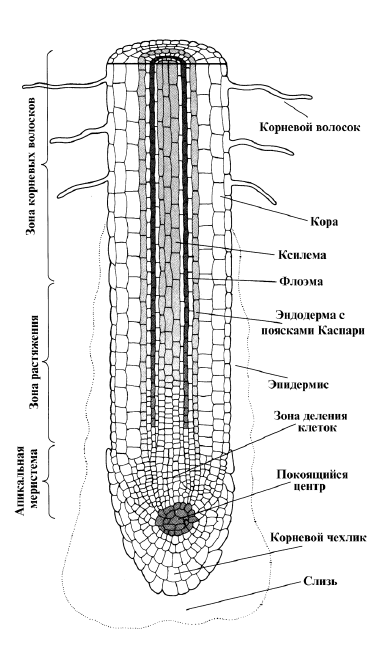
\includegraphics[width=0.8\linewidth]{pictures/root} \\ а) Продольный разрез}
\end{minipage}
\hfill
\begin{minipage}[h]{0.49\linewidth}
\center{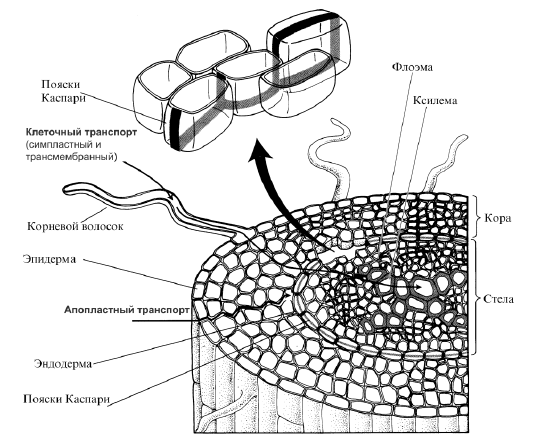
\includegraphics[width=1.2\linewidth]{pictures/root_cross} \\ б) Поперечный разрез}
\end{minipage}
\caption{Схема строения корня}
\paragraph*{}Согласно С.С. Медведева \cite{medvedev_2012}
\label{root_shema}
\end{figure}

%%%%%%%%%%%%%%%%%%%%%%%%%%%%%%%%%%%%%%%%%%%%%%%%%%%%%%%%%%%%%%%%%%%%%%%%%%%%%%

\paragraph*{}Корневая система поглощает воду через корневые волоски, находящиеся в \termin{зоне всасывания}.

\note{Попав в клетку корневого волоска вода становится частью живой системы - клетки растения -- и подчиняется закономерностям, действующим в живой клетке.}

\paragraph*{}Поступление воды в корневую систему растения и перемещение ее по тканям корня осуществляется путем \hyperlink{diffusion}{диффузии}. При этом перемещение воды идет по градиенту ее концентрации.

\paragraph*{}Передвижение по растению определяется двумя основными \termin{двигателями водного потока} в растении:

\begin{enumerate}

\item нижним двигателем водного потока или корневым давлением
\item верхним двигателем водного потока или присасывающим действием атмосферы

\end{enumerate}

\paragraph*{}Действие присасывающей силы корня является причиной таких явлений, как:

\begin{enumerate}

	\item \termin{Гуттация} -- это выделение капельно-жидкой влаги листьями через \termin{гидатоды} в условиях затрудненного испарения (\ris \ref{cry_gutattion} б)
	\item \termin{Плач растения} -- это вытекание \termin{пасоки} (воды с растворенными в ней минеральными веществами, находящейся в ксилеме) из стеблей растений со срезанными побегами (\ris \ref{cry_gutattion} а)

\end{enumerate}

%%%%%%%%%%%%%%%%%%%%%%%%%%%%%%%%%%%%%%%%%%%%%%%%%%%%%%%%%%%%%%%%%%%%%%%%%%%%%%%%%%%%%%%%%%%%%%%%%%%%%%%

\begin{figure}[h]
\begin{minipage}[h]{0.49\linewidth}
\center{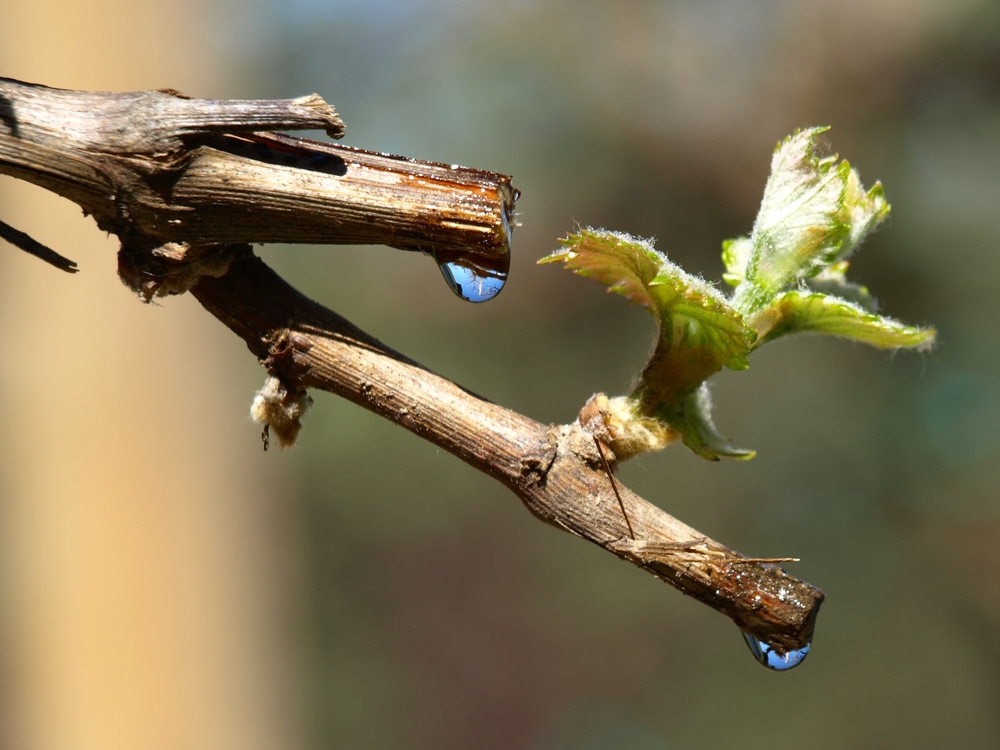
\includegraphics[width=1.1\linewidth]{pictures/cry} \\ а) Плач}
\end{minipage}
\hfill
\begin{minipage}[h]{0.49\linewidth}
\center{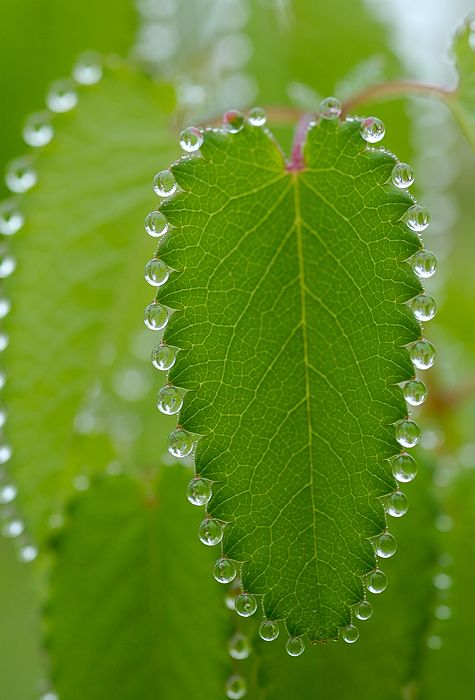
\includegraphics[width=0.55\linewidth]{pictures/guttation} \\ б) Гуттация}
\end{minipage}
\caption{Схема строения корня}

\label{cry_gutattion}
\end{figure}

%%%%%%%%%%%%%%%%%%%%%%%%%%%%%%%%%%%%%%%%%%%%%%%%%%%%%%%%%%%%%%%%%%%%%%%%%%%%%%

\note{Явление гуттации особенно широко распространено в \hyperlink{question_guttation_tropics}{тропиках}, где иногда даже можно попасть под дождь, вызванный гуттирующими растениями \cite{medvedev_2012}}

\note{Состав пасоки сильно варьирует в зависимости от вида растения и фазы его вегетации и фазы органогенеза. Пасока однолетнего травянистого растения и многолетнего древесного растения сильно отличаются друг от друга, так же как и пасока у одного и того же растения весной, летом и осенью. Пасокой являляется березовый сок и кленовый сок. Пасока, выделяющаяся при гуттации, имеет в своем составе очень мало минеральных веществ и сахаров, поскольку происходит их естественная фильтрация при прохождении пасоки через эпитему (ткань, выстилающую воздушную полость гидатоды)}

\subsection*{Передвижение воды по тканям корня}

%\paragraph*{}Вода поглощается корневым волоском как пассивно (по законам осмоса), так и активно. 
\paragraph*{}Различают два пути перемещения воды по тканям корня:

\begin{enumerate}
	\item \termin{Симпластный}, когда вода перемещается по \hyperlink{protoplast}{протопласту} клетки и передается от клетки к клетке через \hyperlink{plasmodesma}{плазмодесмы}
	\item \termin{Апопластный}, когда вода перемещается по межклетникам
\end{enumerate}

\paragraph*{}Проникнув в корневой волосок, далее вода поступает через \termin{эндодерму} в \termin{центральный цилиндр}, где находятся сосуды \hyperlink{qestion_xsilema}{ксилемы и флоэмы}. 

\paragraph*{}Переход воды по клеткам паренхимы корня до эндодермы так же осуществляется по законам осмоса и обуславливается разностью осмотического давления как разных <<полюсов>> одной клетки, так и соседних клеток. При этом, разность осмотического давления внутри клетки создается следующим образом: 

\begin{itemize}

\item В одной части \hyperlink{protoplast}{протопласта} преобладают процессы синтеза осмотически-активных веществ, например \hyperlink{sect_glycosids}{сахаров}. При этом концентрация раствора, а следовательно и осмотическое давление в этой части увеличиваются.
\item Одновременно в другой части клетки протопласта происходит постоянное превращение осмотически активных веществ в осмотически неактивные (например глюкозы в \hyperlink{krahmal}{крахмал}), вследствие чего осмотическое давление в этой части клетки уменьшается.

\end{itemize}

\paragraph*{}Возникающий при этом ток воды обуславливает появление гидростатической силы и передачу воды внутри клетки и от клетки к клетке.


%\paragraph*{}Переход воды внутри клетки и из клетки в клетку обуславливается разностью осмотического давления. 

%Большая часть биоколлоидов клетки принадлежит к гидрофильным соединениям, способным к обратимым изменениям степени своей оводненности. Поглощая воду, коллоидная мицелла набухает, при отдаче же ею воды происходит отбухание. При этом в клетке развиваются весьма значительные силы, достигающие иногда сотен атмосфер.
%Сила, которую нужно приложить к коллоидной системе, чтобы предотвратить поглощение ею воды, называется давлением набухания. Этому свойству биоколлоидов принадлежит важная роль в процессах поглощения протоплазмой воды, в передаче воды в вакуоль и в выделении воды клеткой.
\paragraph*{}Эндодерма является препятствием свободному поступлению воды в центральный цилиндр за счет того, что оболочки эндодермальных клеток сильно утолщены и лигнифицированы. Такие утолщенные оболочки носят название \termin{пояски Каспари} (\ris \ref{root_shema}). Попасть в проводящие ткани центрального цилиндра вода может только через специальные \termin{пропускные клетки} эндодермы, оболочка которых достаточно тонкая. Именно через эти клетки вода под давлением проникает из клеток коры корня в центральный сосудистый цилиндр.

\paragraph*{}Корневое давление зависит от:

\begin{enumerate}

	\item условий влажности почвы (чем больше гидромодуль почвы, т.е. количество воды на единицу площади, тем интенсивнее идет поглощение воды растением),
	\item температуры почвы (ниже 12 \celsius ~и выше 30 \celsius ~поглощение воды замедляется),
	\item аэрации почвы (так как при нарушении аэрации ухудшается процесс дыхания, т.е. получения энергии клеткой, а, значит, и поглощения и передачи воды).

\end{enumerate}

\paragraph*{}Механизм образования корневого давления состоит из двух \hyperlink{question_whater_trans}{аспектов}:

\begin{enumerate}

\item Пассивного переноса воды по законам осмоса
\item Активного, за счет дополнительной сократительной деятельности актомиозиновых белков, находящихся в \termin{перицикле} и \termin{паренхимных клетках} корня.

\end{enumerate}

\subsection*{Передвижение воды по растению}

\note{При передвижении по клеткам паренхимы корня вода обогащается минеральными веществами и в таком составе попадает в клетки ксилемы, скелетной основой которой являются сосуды и трахеиды}.

\paragraph*{}Находящаяся в сосудах и трахеидах вода имеет форму тончайших нитей, которые своими верхними концами как бы подвешены к испаряющим клеткам листьев, а нижними концами упираются в паренхимные клетки корня.

\paragraph*{}Удерживание воды в сосудах ксилемы в виде нитей обуславливается силами:

\begin{itemize}

\item \termin{Когезии} -- прочного \hyperlink{question_water_mol}{сцепление} молекул воды между собой.
\item \termin{Адгезии} -- прилипания молекул воды к гидрофильным стенкам клеток ксилемы.

\end{itemize}

\paragraph*{}Присасывающее действие атмосферы определяется концентрацией водяных паров в атмосфере. Этот показатель в атмосфере почти всегда меньше, чем в листе растения, за исключением условий повышенной влажности воздуха, например, во время дождя, тумана. Присасывающие действие атмосферы объясняется тем, что в атмосфере содержится меньше воды, чем в растении за счет чего образуется отрицательный водный потенциал атмосферы и, следовательно, развивается сосущая сила атмосферы. \gls{suctionPressure} в испаряющих клетках листа достигает 2-4 тысяч к\gls{pascal}.

\subsection*{Транспирация}

\paragraph*{}\hypertarget{transpiration}{\gls{transpiration}} -- это физиологически активный процесс перехода воды в парообразное состояние и диффузию образовавшегося пара в окружающее пространство.

\paragraph*{}Значение транспирации для растения заключается в следующем:

\begin{enumerate}

\item Верхний двигатель тока воды, участвующий в передвижении воды по растению;
\item Испаряющаяся вода охлаждает растение и защищает его от перегрева;
\item Нормализация функционирования коллоидных систем клеток листа;

\end{enumerate}

\note{Таким образом, даже в условиях водного дефицита растение вынужденно транспирировать влагу для того чтобы обеспечить передвижение воды и растворенных в ней веществ по организму. Именно по этому транспирацию иногда называют <<Необходимым злом>>}


\subsubsection*{Водный потенциал как движущая сила транспирации}

\paragraph*{}Движущей силой транспирации является очень большой градиент водный потенциал $\phi$, который создается между атмосферой и воздухом в полости листа

%\remember{Водный потенциал выражает способность воды в данной системе, в том числе в почвенном растворе, в клетке растения, или в атмосфере, совершить работу по сравнению с той работой, которую при тех же условиях совершила бы чистая вода}
	
\paragraph*{}\note{Водный потенциал, являясь мерой активности воды, определяет термодинамически возможное направление ее транспорта. Молекулы воды всегда перемещаются от более высокого водного потенциала к более низкому, подобно тому, как вода течет вниз. Водный потенциал имеет размерность энергии, деленной на объем, поэтому его выражают в барах или паскалях (1 атмосфера = 1,013 бар = $10^{5}$ \gls{pascal}. $10^{6}$ \gls{pascal} равны 1 м\gls{pascal})}

%\paragraph*{}\termin{Химический потенциал воды} $\mu w$ - это величина, производная от активности воды. Она выражает максимальное количество внутренней энергии молекул воды, которое может быть превращено в работу, измеряется в ДЖ. моль$^{-1}$ и рассчитывается по уравнению \ref{chem_pot}:

%\begin{equation}
%	\label{chem_pot}
%	\mu w = \mu w_{0} + RT \ln aw
%\end{equation}

%\paragraph*{}где: $\mu w_{0}$ - химический потенциал чистой воды (принят равным нулю), R - газовая постоянная, T - абсолютная температура, aw - активность воды в системе.

\paragraph*{}В системе <<почвенный раствор -- растение -- атмосфера>> водный потенциал изменяется от самого высокого значения в почвенном растворе до самого низкого в воздухе. \note{Вода переходит из растения в окружающий воздух в парообразном состоянии. В мезофилле листа имеются обширные межклеточные пространства и каждая клетка мезофилла хотя бы одной стороной граничит с таким межклетником. Вследствие испарения воды с влажных клеточных стенок воздух в межклетниках насыщен водяными парами, часть которых через устьица выходит наружу.}

\note{При 100\% влажности воздуха, его водный потенциал равен нулю. Уже при снижении влажности воздуха на 1-2\% его водный потенциал становится отрицательной величиной, а при снижении влажности воздуха до 50\% показатель водного потенциала выражается отрицательной величиной порядка 200-300 бар в зависимости от температуры воздуха. При этом в клетках листьев показатель водного потенциала, как правило, выше нуля, поэтому диффундирование воды из межклетников в атмосферу наблюдается почти всегда.}

\remember{Чем меньше влажность атмосферного воздуха, т.е. чем меньше его водный потенциал, тем интенсивнее будет идти транспирация.} 

\paragraph*{}\gls{transpiration} характеризуется следующими показателями:

\begin{enumerate}

\item \termin{Интенсивность транспирации} -- количество воды, испаряемой растением с единицы листовой поверхности в единицу времени
\item \termin{Продуктивность транспирации} -- это количество созданного сухого вещества на 1 кг транспирированной воды. \note{В среднем эта величина равна 3г/1 кг воды}
\item \termin{Транспирационный коэффициент} -- показывает сколько воды растение затрачивает на построение единицы сухого вещества, т.е. этот показатель является величиной, обратной продуктивности транспирации
\note{В среднем равен 300, т.е. на производство 1 тонны урожая затрачивается 300 тонн воды}

\end{enumerate}

\paragraph*{}Интенсивность транспирации рассчитывается  по следующей формуле \ref{transpiration_level_chpt} 

\begin{equation}
	\label{transpiration_level_chpt}
	T = \frac{10000*C}{St}
\end{equation}

\paragraph*{}Где \textit{T} - интенсивность транспирации, \textit{C} - убыль массы листа за единицу времени; \textit{S} - площадь листа (м$^2$); \textit{t} - время (ч)

\note{Расчету данного показателя посвящена одна из \hyperlink{lab_transp_level}{лабораторных работ}}

\subsubsection*{Механизм работы устьиц}

\paragraph*{}Большая часть воды в растении испаряется через устьица. При этом устьичная транспирация слагается из следующих процессов:

\begin{enumerate}
	\item Передвижение воды из сосудов в клеточные стенки клеток мезофилла листа
	\item Испарение воды с поверхности клеток мезофилла
	\item Диффузия водяных паров в межклеточных пространствах рыхлого мезофилла
	\item Выход воды через устьица
\end{enumerate}

\paragraph*{}Замыкательные клетки устьиц -- это единственные клетки в эпидермисе листа, содержащие хлоропласты так как механизм открывания устьиц связан с процессом фотосинтеза. В основе процесса открытия устьиц лежит следующая цепочка событий:

\begin{enumerate}
	\item На свету в хлоропластах замыкательных клеток устьиц начинается процесс синтеза сахаров. В следствии этого осмотическое давление внутри клетки возрастает
	\item Из соседних клеток в замыкательные клетки устьица начинает поступать вода
	\item В следствии этого внутри замыкательных клеток возрастает \gls{turgor}
	\item Так как клеточная стенка замыкательной клетки устьица утолщена неравномерно, из за повышения тургорного давления замыкательные клетки выгибаются, открывая, тем самым, устьичную щель. \note{За счет эластичности клеточной стенки, замыкательные клетки устьиц могут увеличиваться на 40--100\% \cite{medvedev_2012}}
\end{enumerate}

\subsubsection*{Влияние различных факторов на интенсивность транспирации}

\paragraph*{}На интенсивность транспирации наиболее существенное влияние оказывают следующие факторы:

\begin{enumerate}
	\item Температура воздуха. Чем выше температура воздуха, тем выше будет и температура листа, при этом температура внутри клеток листа может быть на 10 \celsius выше, чем в атмосфере. Происходит нагрев воды, находящейся в листе, что также способствует процессу испарения.
	\item Влажность воздуха. С ростом относительной влажности воздуха, интенсивность транспирации падает.
	\item Концентрация углекислого газа в подустьичной полости. Чем ниже концентрация, т.е. меньше 0,03\%, находящихся в воздухе, тем больший приток воды в замыкающие клетки устьица и тем шире устьичная щель,
	\item Наличие солнечного света. На свету крахмал превращается в простые сахара, т.е. концентрация клеточного сока выше, поэтому наблюдается больший приток воды в замыкающие клетки устьица и раскрытие устьичной щели. Наибольшую роль для открывания устьиц играет \termin{синий} свет.
	\item Скорость ветра. Непосредственно к испаряющей поверхности прилегает слой воздуха, в котором водяной пар постепенно испаряется далее в атмосферу, при этом в безветренную погоду скорость испарения выражается линейной зависимостью между дефицитом насыщения воздуха и расстоянием от испаряющей поверхности. Однако, при наличии ветра, который <<сдувает>> испаряющиеся молекулы воды, происходит увеличение дефицита насыщения воздуха и увеличение интенсивности транспирации
	\item Количество устьиц на единицу площади листа
	\item Форма листа листа
	\item Наличие ионов $К^{+}$. Чем выше концентрация, тем больший приток воды в замыкающие клетки устьица и тем шире устьичная щель
	\item Наличие абсцизовой кислоты. Чем выше концентрация этого гормона, тем меньше раскрытие устьица \note{Например - мутант томата wilty}
\end{enumerate}

\paragraph*{}Суточный ход транспирации у всех растений определяется максимальной транспирацией в утренние часы и минимальной -- в полуденные. При этом на интенсивность транспирации существенное влияние оказывают такие факторы, как:

\begin{enumerate}

	\item температура почвы и воздуха, 
	\item влажность почвы и воздуха, 
	\item интенсивность солнечного излучения, 
	\item наличие ветра.

\end{enumerate}

\paragraph*{}Сезонный ход транспирации у многолетних растений определяется фазами развития растения.

\subsection*{Водный баланс в растении}

\remember{Водный баланс в растении поддерживается тогда, когда скорость поглощения воды равна скорости ее испарения}

\paragraph*{}Обычно водный баланс в растении меняется в течение суток, зависит от уровня агротехники при выращивании растений.

\paragraph*{}Важной характеристикой водного баланса является \termin{степень оводненности тканей растения}. Этот показатель рассчитывается по формуле \ref{water_level}.

\begin{equation}
	S = \frac{m_{w}-m_{dr}}{m_{w.f}-m_{dr}}*100
	\label{water_level}
\end{equation}

\paragraph*{}Где S -- степень оводненности тканей, $m_{w}$ -- масса образца сырой ткани, $m_{dr}$ -- масса образца сухой ткани, $m_{w.f}$ -- масса сырой ткани в состоянии полного насыщения.

\note{У большинства мезофитов степень оводненности составляет 85—95\%. Если поглощение и потребление воды растением сбалансированы, степень оводненности
не меняется. Если оводненность меньше 50\%, то ткани начинают отмирать. Поэтому растения стремятся регулировать потоки воды таким образом, чтобы поддерживать оводненность клеток и тканей на необходимом уровне \cite{medvedev_2012}.}


\paragraph*{}Несбалансированность поступления и испарения воды проявляется в наличии \termin{водного дефицита}, который наблюдается, как правило, у растений днем и отсутствует ночью.

\paragraph*{}В практике сельского хозяйства используются приемы, снижающие водный дефицит у растений. Как правило эти приемы заключаются в использовании: 

\begin{enumerate}
	\item Освежительных поливов
	\item Антитранспирантов
\end{enumerate}

\paragraph*{}Антитранспиранты делятся на две разновидности веществ:

\begin{enumerate}
	\item вызывающие закрытие устьиц (абсцизовая кислота, фенилмеркурацетат),
	\item образующие пленки на листьях (полиэтилен, латекс).
\end{enumerate}


\subsection*{Вопросы и задания для самоконтроля}

\begin{enumerate}
	\item Что такое осмос и \hypertarget{osmosis}{осмотическое давление}. От каких факторов зависит величина осмотического давления? Информацию о природе осмоса можно повторить по учебнику физической и коллоидной химии А.Г. Стромберга \cite{stromberg_2006}.
	\item Какой из двух \hypertarget{question_whater_trans}{механизмов} переноса воды в корне -- осмотический или перенос с помощью белков можно отнести к активным, а какой к пассивным явлениям? Почему?
	\item Воспользовавшись учебником по ботанике, например за авторством И.И. Андреевой \cite{andreeva-bot}, повторите строение проводящих тканей. В чем состоят особенности строения и функционирования клеток \hyperlink{qestion_xsilema}{ксилемы} и флоэмы?
	\item Воспользуйтесь учебником химии и повторите строение \hypertarget{question_water_mol}{молекулы воды}. За счет каких особенностей строения, молекулы воды способны образовывать друг с другом непрочные водородные связи?
	\item Как вы считаете, почему гуттация так широко распространена именно в \hypertarget{question_guttation_tropics}{тропиках}?
\end{enumerate}
	
	\section{Фотосинтез}
	
	%Лекция 5. Фотосинтез. Световая стадия фотосинтеза

%\subsection*{История изучения фотосинтеза}

%\begin{enumerate}

%\item количественные эксперименты Ван Гельмонта (начало XVII в.) по выращиванию ивы на песке 
%\item опыты Дж. Пристли в 1771 г. показали способность зеленых растений выделять на свету кислород. 
%\item Бойер вывел стехиометрическое уравнение фотосинтеза 
%\item А.Н. Бах (1857–1946) установил, что фотосинтез представляет собой серию сопряженных окислительно-восстановительных реакций, в результате которых происходят как усвоение углекислого газа, так и освобождение кислорода из воды с участием перекиси в качестве промежуточного продукта. 
%\item В 1905 г. Ф. Блекман сформулировал фундаментальное положение: <<Фотосинтез состоит из световой и темновой фаз>>. 

%\end{enumerate}

%\subsection*{Роль фотосинтеза в процессах энергетического и пластического обмена растительного организма}
%У водорослей и высших растений основными конечными продуктами фотосинтеза являются углеводы (чаще сахароза и крахмал). Крахмал накапливается в фотосинтезирующих клетках в виде крахмальных зерен. В целом, продукты фотосинтеза относятся к
%углеводам, 
%органическим кислотам и 
%аминокислотам. 

\subsection*{Масштабы фотосинтетической деятельности в биосфере}

\paragraph*{}\hypertarget{photosyntesis}{\Gls{photosyntesis}} -- это процесс синтеза органических веществ из неорганических при участии \gls{chlorophill}а и за счет энергии солнца.

\paragraph*{}В процессе фотосинтеза на Земле первично создаются органические вещества. \Gls{photosyntesis} включен в глобальный газообмен на планете, обеспечивая необходимый для жизни уровень кислорода, а также необходимый для биосферы в целом уровень углекислого газа.

%\note{Основная масса (примерно 57 \%) углекислоты атмосферы имеет растительное происхождение. Почва в результате жизнедеятельности почвенных микроорганизмов поставляет около 58 млрд. т углекислоты в год, то есть 38 \%. Промышленная деятельность человечества (сжигание угля, нефти и другие) занимает 3 \% в балансе выделяемой углекислоты. Остальные источники - дыхание людей и животных, вулканы, фумаролы и другие - вместе выделяют менее 2 \% углекислоты. }

\note{Ежегодно в процессе фотосинтеза наземные и морские растения поглощают около 15,6 х $10^{10}$ т углекислоты, то есть 1/16 всего мирового запаса. В среднем на 1 $км^{2}$ суши приходится 110 т. углерода в год. Одна тонна органического углерода аккумулирует приблизительно 107 ккал световой энергии. Это составляет 0,02–0,03 \% от световой энергии в области \gls{phtr}. Определяющими состояние биосферы параметрами являются количество запасенного органического вещества (валовая первичная продукция), количество выделившегося кислорода, балансовый уровень углекислого газа в атмосфере (глобальная температура, глобальный климат).}

\subsection*{Краткий систематический обзор фотосинтетиков}

\paragraph*{}Фотосинтетики -- это \gls{avtotrophicOrg} организмы, встречаются 
в: 

\begin{enumerate}

	\item надцарстве Доядерных организмов (Procaryota): 

		\begin{itemize}

			\item подцарствах Бактерии (Bacteriobionta) и 
			\item подцарство Цианеи (Cyanobionta)\footnote{Раньше цианей называли сине-зелеными водорослями. Однако использовать слово водоросли применительно к данной группе неправильно, так как водоросли это эукариотические организмы, а цианеи -- прокариотические}. В качестве фотосинтетического пигмента присутствует \gls{chlorophill} А. Дополнительные пигменты -- фикобилины.

		\end{itemize}
 
	\item в надцарстве Ядерные организмы (Eucaryota),

		\begin{itemize}

			\item царстве Растений (Plantae): 

				\begin{itemize}

						\item подцарства Багрянок (Rhodobionta). Пигменты представлены \gls{chlorophill}ом А, редко хлорофиллом D, фикоэритрином и фикоцианином, но без хлорофилла C; 
						\item Настоящих водорослей (Phycobionta). В качестве пигментов присутствуют хлорофиллы (A+C) (A+B), но без хлорофилла D
						\item \hypertarget{embryobionta}{Высших растений} (Embryobionta). В качестве пигментов присутствуют хлорофиллы (A+C) (A+B), но без хлорофилла D;

				\end{itemize}

		\end{itemize} 

\end{enumerate}
 
%Основные балансовые уравнения фотосинтеза
%У зеленых растений водорослей и цианобактерий: донор водорода – вода.
%СО2 + 2Н2О → (СН2О) + О2 + Н2О,
%где (СН2О) – условное обозначение образующегося при фотосинтезе органического вещества (1/6 часть молекулы глюкозы). 
%У пигментированных серобактерий: донор водорода сероводород:
%СО2 + 2Н2S → (СН2О) + 2S + Н2О 
%Когда сероводород почти исчерпан, бактерии начинают окислять серу до сульфатов
%3СО2 + 2S + 5Н2О → 3 (СН2О) + 2 Н2SО4.
%В минерализованных водах, где распространены пурпурные и зеленые серные бактерии, серная кислота вступает в реакции с ионами металлов, образуя сульфаты. 

\subsection*{Структурная организация фотосинтетического аппарата прокариот и эукариот}

%\paragraph*{}Процесс фотосинтеза протекает в специализированных клетках с фотосинтетическими пигментами. 
\paragraph*{}Клетки прокариот -- наиболее просто организованные автономные фотосинтезирующие структуры. Фотосинтетические пигменты и белки электрон-транспортной цепи у этих организмов не обособлены в специальных органеллах, а встроены в \hyperlink{plasmolema}{клеточную мембрану}. При этом, в отсутствие света белки фотосинтеза могут переключаться на \hyperlink{sect_breazing}{дыхание}. У цианобактерий тилакоиды заполняют большую часть клетки и не организованы в граны. 

\paragraph*{}Фотосинтезирующие же клетки эукариот обязательно имеют в своем составе органеллы -- \hyperlink{cell_plastids}{хлоропласты} или хроматофоры. Хлоропласты способны выполнять весь комплекс процессов фотосинтеза, связанных с поглощением света, и основную часть ферментативных реакций, обеспечивающих ассимиляцию углекислого газа. 

\paragraph*{}Весь комплекс ферментативных реакций фотосинтеза требует кооперации хлоропластов (кооперативный фотосинтез у С4 – растений) или хлоропластов, \hyperlink{mitohondria}{митохондрий}, глиоксисом и пероксисом (у С3 – растений при фотодыхании).

%Хлоропласты имеют форму эллипсоида, окружены двойной мембраной. Внутри хлоропласта расположены пигментсодержащие мембраны, образующие замкнутые полости - тилакоиды. Свободное от тилакоидов пространство внутри хлоропласта - строма. Собранные в «стопки» тилакоиды образуют граны. 

\subsubsection*{Пигменты фотосинтеза}

\paragraph*{}Основным пигментами участвующими в фотосинтезе являются хлорофиллы. \hypertarget{sect_hlorophilus}{\gls{chlorophill}ы} -- это целая группа пигментов. У высших растений присутствуют, как было сказано \hyperlink{embryobionta}{выше}, хлорофиллы А, B, C и D. 

\paragraph*{}Эмпирическая формула хлорофилла A -- $C_{55}H_{72}O_{5}N_{4}Mg$.

\paragraph*{}Молекула хлорофилла (\ris \ref{hlorophilus_molecula}) состоит из: 

\begin{enumerate}

\item \termin{Порфиринового кольца} (тетрапиррола);
\item Дикарбоновой кислоты -- \termin{хлорофиллина}, \hyperlink{eterefication}{этерифицированной} остатком метилового спирта;
\item Высокомолекулярного одноатомного спирта -- \termin{фитола};

\end{enumerate}

%MgN4OH30C32 – COOC20H39(COOCH3).

\note{У хлорофилла B в пиррольном кольце II метильная группа при С3 заменена альдегидной. Его эмпирическая формула -- $C_{55}H_{70}O_{6}N_{4}Mg$.} 

%%%%%%%%%%%%%%%%%%%%%%%%%%%%%%%%%%%%%%%%%%%%%%%%%%%%%%%%%%%%%%%%%%%%%%%%%%%%%%%%%%%%%%%%%%%%%%%%%%%%%%%

\begin{figure}[h]
\begin{minipage}[h]{0.49\linewidth}
\center{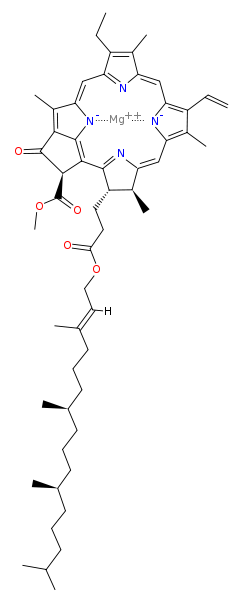
\includegraphics[width=0.5\linewidth]{pictures/hla} \\ a) Хлорофилл A}
\end{minipage}
\hfill
\begin{minipage}[h]{0.49\linewidth}
\center{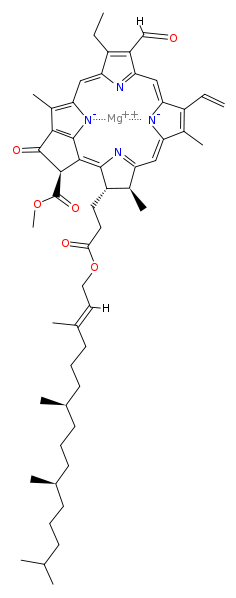
\includegraphics[width=0.5\linewidth]{pictures/hlb} \\ б) Хлорофилл Б}
\end{minipage}
\caption{Схема строения молекулы хлорофилла}

\label{hlorophilus_molecula}
\end{figure}

%%%%%%%%%%%%%%%%%%%%%%%%%%%%%%%%%%%%%%%%%%%%%%%%%%%%%%%%%%%%%%%%%%%%%%%%%%%%%%

%\note{Хлорофилл D дополняет хлорофилл A у некоторых красных и хризофитовых водорослей. Хлорофилл D можно рассматривать как производную от хлорофилла A, в молекуле которого винильная группа при С2 заменена на формильную группу}

\paragraph*{Химические свойства хлорофилла}

\paragraph*{}Ядро хлорофилла обладает гидрофильными свойствами а остаток фитола -- гидрофобными свойствами. Это позволяет молекуле хлорофилла взаимодействовать как с белками, так и с липидами. 

\paragraph*{}Хлорофиллы легкорастворимы в ацетоне, серном эфире, этаноле, метаноле, сероуглероде, бензоле, плохорастворимы в петролейном эфире.

\paragraph*{}При потере магния хлорофилл превращается в \termin{феофитин}, магния и фитола -- в \termin{феофорбид}, только фитола -- в \termin{хлорофиллид}.

\paragraph*{}Рассмотрению химических свойств хлорофилла будет посвящена одна из \hyperlink{chem_hlorophil}{лабораторных работ}.

\note{Окраска хлорофила настолько интенсивная, что на покраску одного гектара тропического леса понадобилось бы лишь одно ведро хлорофилла}

\paragraph*{}Различные типы хлорофилла отличаются и по длине волны поглощаемого света:

\begin{enumerate}

\item Максимумы поглощения хлорофилов A и B лежат в синей части спектра (полоса Соре) 428,5-430 нм и 452,5-455 нм и в красной части спектра 660-662 нм и 642-649 нм (\ris \ref{hlspectr})
\item Максимумы поглощения хлорофилла C (в 80 \% ацетоне) -- 446 нм и 631 нм. 
\item Максимумы поглощения хлорофила D (в диэтиловом эфире) -- 445 нм и 686 нм.

\end{enumerate}

%%%%%%%%%%%%%%%%%%%%%%%%%%%%%%%%%%%%%%%%%%%%%%%%%%%%%%%%%%%%%%%%%%%%%%%%%%%%%%%%%%%%%%%%%%%%%%%%%%%%%%%%%%% 
\begin{figure}
  \centering
       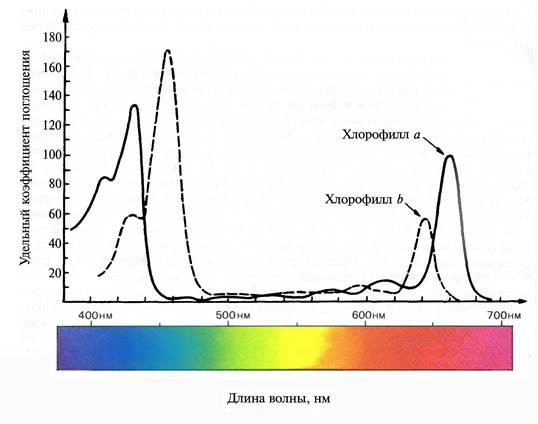
\includegraphics[width=0.6\linewidth]{pictures/hlspectr}
\caption{Спектры поглощения хлорофиллов}
\label{hlspectr}
\end{figure}
%%%%%%%%%%%%%%%%%%%%%%%%%%%%%%%%%%%%%%%%%%%%%%%%%%%%%%%%%%%%%%%%%%%%%%%%%%%%%%%%%%%%%%%%%% 

\paragraph*{}Таким образом, <<полезным>> для фотосинтеза является только свет с определенной длинной волны.

\remember{Та часть солнечного спектра, которая способна возбудить молекулу хлорофилла называется \gls{phtr}}


\note{В физиологических исследованиях важным показателем является отношение вспомогательных хлорофиллов (B, C, D) к хлорофиллу A, которое характеризует степень адаптации к низкому уровню облученности.}

\paragraph*{}Структура молекулы хлорофилла такова, что хлорофилл является хорошим \termin{сенсибилизатором} -- то есть под действием света хлорофилл легко возбуждается и способен вступать в окислительно-восстановительные реакции. Легкость, с которой молекула хлорофилла переходит в возбужденное состояние объясняется системой \hyperlink{question_bounds}{сопряженных} кратных связей в порфириновом кольце.

\subsubsection*{Фотосинтетическая единица}


\paragraph*{}В выделении одной молекулы кислорода в процессе фотосинтеза участвуют не одна, а сразу множество молекул хлорофилла, функционирующие совместно. Эта совокупность молекул получила название \termin{фотосинтетическая единица}. У высших растений в состав \hyperlink{question_photo_unit}{фотосинтетической единицы} обычно входит от 200 до 400 молекул хлорофилла. Таким образом, свет поглощается сотнями молекул хлорофилла, которые затем переносят свою энергию возбуждения к тому месту, где протекают химические реакции. Это место называется \termin{реакционным центром}. 

\paragraph*{}В составе фотосинтетической единицы выделяют два функциональных типа фотосинтетических пигментов:

\begin{itemize}

	\item поглощающие и передающие энергию возбуждения: антенные комплексы
	\item первичные фотохимические реакции: реакционные центры


\end{itemize}

%\paragraph*{}Таким образом, функция большинства молекул хлорофилла в фотосинтетической единице состоит в поглощении света. Только малая доля хлорофиллов, те, которые локализованы в реакционных центрах, участвует в преобразовании света в химическую энергию. 

\note{Хлорофиллы в реакционном центре химически идентичны другим хлорофиллам фотосинтетической единицы, но обладают особыми свойствами, обусловленными их особым окружением. Одно из различий состоит в том, что энергетический уровень возбужденного состояния хлорофиллов реакционного центра ниже, чем у других хлорофиллов, и они поэтому способны улавливать энергию \cite{stier_85}} 

\paragraph*{}Энергия, поглощенная молекулами хлорофилла, перемещается по фотосинтетической единице, пока не достигнет хлорофилла \termin{реакционного центра}. Фотохимическую функцию в составе реакционных центров выполняет хлорофилл A.

\subsubsection*{Реакционные центры}

\paragraph*{}Реакционные центры находятся в центре особых белковых комплексов -- \hypertarget{photosystems}{фотосистем}, интегрированых в мембрану \hyperlink{cell_plastids}{тилакоидов}. 

\paragraph*{}\gls{photosystem} представляет собой функциональную и структурную единицу белковых комплексов, которые осуществляют первичные фотохимические реакции фотосинтеза: поглощение света, преобразование энергии и перенос электронов. 

\paragraph*{}Различают два типа фотосистем -- \gls{fs1} и \gls{fs2}. В \hyperlink{cell_plastids}{хлоропластах} растений присутствуют и \hyperlink{photocooperation}{согласованно} работают оба этих типа фотосистем.

%Первичный акцептор электрона – убихинон в окисленном состоянии тушит флюоресценцию хлорофилла а в составе светособирающего комплекса ФС2. 

\paragraph*{}Реакционным центром \gls{fs1} является длинноволновая форма хлорофилла а с максимумом поглощения при 700 нм ($P_{700}$). 

\paragraph*{}Антенный комплекс \gls{fs2} состоит из 36 молекул хлорофилла A, комплекс \gls{fs1} -- из 96 молекул. Размеры светособирающего комплекса не постоянны и зависят от условий, в которых формируется и функционирует фотосинтетический аппарат.

\remember{Результатом работы реакционных центров является разделение зарядов (отрицательный заряд на внутренней поверхности, мембраны  положительный -- на внешней).} 

\subsubsection*{Электрон-транспортная цепь фотосинтеза}

\paragraph*{}Компоненты \hypertarget{photoetl}{фотосинтетической цепи} переноса электронов локализованы в мембране \hyperlink{cell_plastids}{тилакоидов} (\ris \ref{etl})

%%%%%%%%%%%%%%%%%%%%%%%%%%%%%%%%%%%%%%%%%%%%%%%%%%%%%%%%%%%%%%%%%%%%%%%%%%%%%%%%%%%%%%%%%%%%%%%%%%%%%%%%%%% 
\begin{figure}
  \centering
       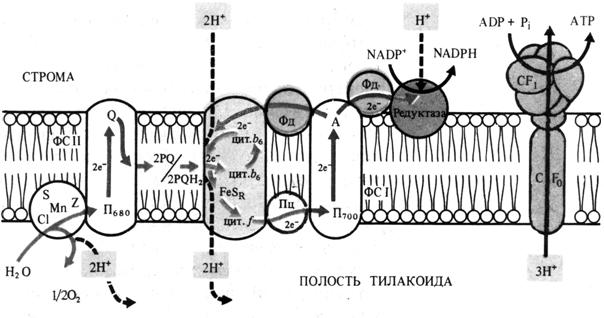
\includegraphics[width=0.8\linewidth]{pictures/etl}
\caption{Схема расположения белков электрон-транспортной цепи на мембране}
\label{etl}
\end{figure}
%%%%%%%%%%%%%%%%%%%%%%%%%%%%%%%%%%%%%%%%%%%%%%%%%%%%%%%%%%%%%%%%%%%%%%%%%%%%%%%%%%%%%%%%%% 

\paragraph*{}Различают следующие компоненты электрон-транспортной цепи:

\begin{enumerate}
	\item Цитохромный комплекс белков-переносчиков электронов, в который входят 2 \gls{cytochrom}а $b_{6}$, \gls{cytochrom} f и железосерный белок Риске FeSR.
	\item Белок ферродоксин, который находится поверхности мембраны со стороны стромы
	\item \hyperlink{enzimes}{Фермент} ФАД-редуктаза, белок пластоцианин, который расположен со стороны просвета \hyperlink{cell_plastids}{тилакоида}.
\end{enumerate}

\paragraph*{}Последовательность переносчиков электронов в \gls{electonykLink} фотосинтеза определяют на основе величины их окислительно-восстановительного потенциала. 

\remember{Электрон самостоятельно может переходить от донора к акцептору, если редокс-потенциал донора (ЕД) меньше, чем редокс-потенциалом акцептора (ЕА). В противном случае перенос электрона происходит в результате фотохимической реакции за счет энергии света.}

\paragraph*{}В цепи транспорта электрона выделяют пять \hyperlink{proteins}{белковых комплексов}, дифференцированных структурно и функционально: 

\paragraph*{}Таким образом, фотосинтетический аппарат растения включает в себя следующие компоненты:

\begin{enumerate}

	\item \gls{fs2}, состоящая из 

		\begin{enumerate}
			\item Хлорофилл $P_{680}$, 
			\item Переносчики электронов -- феофитин, хиноны Q a и $Q_{b}$. 
		\end{enumerate} 

	\item \gls{fs1}, состоящая из 

		\begin{enumerate}
			\item Хлорофилл $P_{700}$, 
			\item переносчики электронов $A_{0}$ (хлорофилл), $A_{1}$ (филлохинон витамин К), 3 железосерных белка FeS
		\end{enumerate}
	
	\item \gls{electonykLink}
\end{enumerate}


\subsection*{Световая фаза фотосинтеза}

\paragraph*{}\termin{\hypertarget{light_stage}{Световая фаза}} -- это этап фотосинтеза, в течение которого за счёт энергии света образуются богатые энергией соединения \gls{atp} и молекулы — носители энергии.

\paragraph*{}Осуществляется на внутренних мембранах \hyperlink{cell_plastids}{хлоропластов}, на которых располагаются молекулы хлорофилла и представляет собой последовательность из фотофизических и фотохимических процессов.

\paragraph*{}В фотофизических реакциях передачи энергии между пигментами и в фотохимических реакциях передачи электронов принимают участие возбужденные молекулы пигментов. У хлорофиллов, фикобилинов и каротиноидов при поглощении кванта света в возбужденное состояние переходят $\pi$-электроны, участвующие в образовании двойной связи.

\subsubsection*{Поглощение света и передача энергии возбуждения}

\paragraph*{}\hyperlink{question_chem_phys}{Преобразование} световой энергии в химическую энергию продуктов фотосинтеза происходит в следующей последовательности.

\begin{enumerate}

\item На первой, \termin{фотофизической} стадии квант света поглощается молекулами хлорофилла и направляется в реакционный центр
\item В реакционном центре происходит следующая стадия -- \termin{фотохимическая}, в результате которой энергия возбужденной молекулы хлорофилла расходуется на разделение зарядов энергия в реакционном центре. 

\remember{Разделение зарядов -- это ключевое событие фотосинтеза, потому что именно на этом этапе происходит преобразование физической формы энергии в химическую \cite{medvedev_2012}}

\item На третьем этапе, в результате \termin{фотохимических} процессов осуществляется синтез \gls{atp} и \gls{nadfh2}, которые являются главными продуктами световой стадии фотосинтеза.

\end{enumerate} 

\paragraph*{}В последующем, энергия, запасенная в продуктах световых реакций используется в темновой (физиологической) фазе фотосинтеза и расходуется на синтез органических соединений и регенерацию акцептора углекислого газа.

\remember{Процесс синтеза \gls{atp} за счет энергии света в процессе световой стадии фотосинтеза называется \hypertarget{photophosforolysis}{фотофосфорилирование}}

\paragraph*{}Различают два пути фотофосфорилирования:

\begin{enumerate}
	\item Циклическое
	\item Нециклическое
\end{enumerate}

\subsubsection*{Циклическое фосфорелирование}

\paragraph*{}Циклическое фотофосфорилирование -- это более простой эволюционно древний путь. В нем участвует \gls{fs1} и цитохромный комплекс и его единственным продуктом является \gls{atp}.

\paragraph*{}При поглощении 2 квантов света хлорофилл $Р_{700}$ переходит в возбужденное состояние и отдает 2 электрона, трем железосерным белкам (FeS). Попав в электрон-транспортную цепь электроны движутся по ее белкам в следующей последовательности: ферридоксину $\rightarrow$ пластохиноны PQ внутри мембраны $\rightarrow$ \gls{cytochrom}ы b6 $\rightarrow$ железосерный белок Риске FeSR $\rightarrow$ пластоцианин. С пластоцианина электрон опять возвращается к молекуле $Р_{700}$. Освобождающаяся энергия используется для синтеза одной молекулы \gls{atp}.

\paragraph*{}Таким образом, электрон движется по кругу -- он выбивается светом из хлорофилла и затем, пройдя по цепи переносчиков возвращается в эту же молекулу.

\subsubsection*{Нециклическое фосфорелирование}

\paragraph*{}При нециклическом фосфорилировании $P_{680}$, поглотив 2 кванта света, переходит в возбужденное состояние и отдает 2 электрона феофитину, затем электроны передает последовательно по следующей цепи из белков хиноны $Q_{a}$ и $Q_{b}$, $\rightarrow$ пластохиноны PQ внутри мембраны $\rightarrow$ железосерный белок FeSR $\rightarrow$ \gls{cytochrom} f $\rightarrow$ пластоцианин и $Р_{700}$ (\ris \ref{acyclfosph}).

\paragraph*{}Молекула хлорофилла $P_{700}$, поглотив 2 кванта света, переходит в возбужденное состояние и отдает 2 электрона, трем железосерным белкам (FeS) $\rightarrow$ ферридоксину $\rightarrow$ ферменту ФАД-редуктазе, которая восстанавливает \gls{nadfh2}. 

\paragraph*{}Недостающие электроны в $P_{700}$ переходят с пластоцианина.

\paragraph*{}Энергия, освобождающаяся при движении электронов от $P_{680}$ (Е=-0,8В)
до $P_{700}$ (Е=+0,4В) используется для синтеза 3 \gls{atp}.

\paragraph*{}Таким образом, при нециклическом фосфорилировании обе фотосистемы \hypertarget{photocooperation}{работают} \hyperlink{question_photocooperation}{согласованно}.

%%%%%%%%%%%%%%%%%%%%%%%%%%%%%%%%%%%%%%%%%%%%%%%%%%%%%%%%%%%%%%%%%%%%%%%%%%%%%%%%%%%%%%%%%%%%%%%%%%%%%%%%%%% 
\begin{figure}
  \centering
       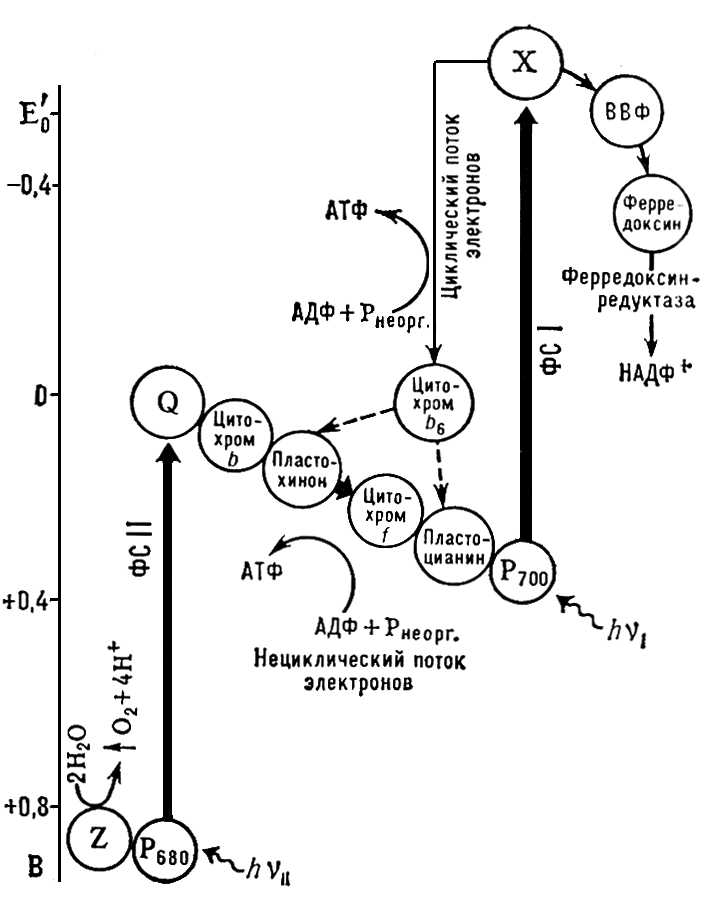
\includegraphics[width=0.4\linewidth]{pictures/acyclfosph}
\caption{Схема ациклического пути фотосинтеза}
\label{acyclfosph}
\end{figure}
%%%%%%%%%%%%%%%%%%%%%%%%%%%%%%%%%%%%%%%%%%%%%%%%%%%%%%%%%%%%%%%%%%%%%%%%%%%%%%%%%%%%%%%%%% 



%\subsubsection*{Совместное функционирование двух фотосистем}

%\paragraph*{}Перенос электронов против термодинамического градиента от воды к НАДФ+ ($\delta E \approx 1,15$ В) происходит за счет энергии двух квантов света с участием двух фотосистем, работающих последовательно. 
%Красное падение (Первый эффект Эмирсона). Квантовый выход снижается в спектральной области, которую поглощают каротиноиды, а также в области длин волн больше 685 нм, в которой интенсивно поглощается хлорофилл а, но не поглощается хлорофилл в. 
%Эффект усиления (Второй эффект Эмирсона). Эффект <<красного падения>> может быть снят при добавочном освещении более коротковолновым светом, поглощаемым хлорофиллом b или каротиноидами.  

\note{Процесс фотофосфорилирования продолжается даже при отрицательных температурах}

\subsubsection*{Фотоокисление воды}

\note{Как было сказано выше, в ходе нециклического фосфорилирования молекула хлорофилла $Р_{700}$ теряет свой, поэтому клетке растения необходим источник электронов, с помощью которого хлорофилл $Р_{700}$ мог бы восполнять потерянные электроны. Таким источником является фотолиз или фотоокисление воды.}

\paragraph*{}Комплекс \hypertarget{photolisys}{фотоокисления} воды интегрирован в белок в составе \gls{fs2}. Реакции фотоокисления воды протекают на внутренней стороне мембран тилакоида. 

\paragraph*{}В общем виде реакция фотоокисления воды идет по следующей схеме:

\paragraph*{}$2H_{2}O \xrightarrow{\text{4 кванта света}} 4H^{+} + 4e + O_{2}$.

\paragraph*{}Таким образом, после удаления четырех электронов из воды образуется молекулярный кислород. Состав каталитического центра, участвующего в фотоокислении $Mn_{4}O_{4}Ca$. В качестве кофактора реакции фотоокисления воды выступают ионы хлора. 

\remember{Именно фотоокисление воды является источником молекулярного кислорода, выделяемого растениями}

\subsubsection*{Стехиометрия сопряжения электронного транспорта и образования АТФ}

\paragraph*{}Фосфорилирование представляет собой процесс синтеза молекулы АТФ из пирофосфата и АДФ за счет свободной энергии, освобождающейся в ходе сопряженной химической реакции, или за счет электрохимического потенциала ионов водорода. 

\note{Поскольку накопление электрохимического градиента в тилакоидах происходит за счет энергии света, синтез \gls{atp} в хлоропластах получил название фотосинтетического фосфорилирования, или фотофосфорилирования.}

\paragraph*{}Реакция синтеза \gls{atp}, катализируемая локализованной в мембране обратимой АТФазой, 
%АДФ + Фн + 3Н+внутр = АТФ + Н2О + 3Н+внешн.

\paragraph*{}Энергетически зависимая стадия синтеза \gls{atp} представляет собой отщепление образованной \gls{atp} от энзимного комплекса.

\note{Образование \gls{atp} в хлоропластах можно вызвать в темноте за счет искусственного создания протонного градиента в условиях кислот-основного перехода. В единицах рН величина градиента ионов водорода, необходимая для синтеза \gls{atp}, составляет 3-3,5 ед. При этом рН стромы составляет величину порядка 7,8-8,0, рН внутри тилакоида -- 4,0-4,5 ед.}
%Электрохимический градиент ионов водорода направлен из внутритилакоидного пространства в строму. Концентрационная составляющая электрохимического градиента существенно превалирует над электрической составляющей. Это достигается выходом из тилакоидов ионов калия и магния.

\paragraph*{}Градиент электрохимического потенциала ионов водорода на мембране тилакоида возникает в результате: 

\begin{enumerate}

\item выхода \gls{proton}ов во внутреннее пространство тилакоида при фотоокислении воды, 
\item связывании ионов водорода в пространстве стромы при восстановлении акцептора электронов \gls{nadfh2}, 
\item транспорта \gls{proton}ов посредством подвижного переносчика – пластохинона.

\end{enumerate}


\subsection*{Темновая стадия фотосинтеза}

\paragraph*{}На темновой стадии\footnote{Темновая стадия -- это традиционное название, не совсем точно отражающее суть процесса. Првильнее было бы называть эту стадию светонезависимой. Реакции темновой стадии не нуждаются в энергии света, однако нуждаются в продуктах световой стадии, поэтому эти реакции не могут идти в темноте, когда продукты световой стадии не вырабатываются}, поглощаемый растениями углекислый газ связывается с различными сахарами. Итогом этой реакции является образование пировиноградной кислоты, а затем и глюкозы.

%Природа первичных акцепторов углекислого газа (углекислоты) Акцептором углерода следует считать органическую молекулу, способную ферментативным путем присоединить молекулу углекислого газа (СО2) или остаток угольной кислоты (НСО3-1, СО3-2). 
\paragraph*{}Процесс присоединения молекулы $CO_{2}$ к органическому соединению с образованием карбоксильной группы называют \termin{карбоксилированием}, а \hyperlink{enzimes}{ферменты}, осуществляющие этот процесс, -- \termin{карбоксилазами}. 

\paragraph*{}Карбоксилирование свойственно как гетеротрофным, так и автотрофным организмам. 

\paragraph*{}Источником энергии для карбоксилирования является \gls{atp}, накопленная во время световой стадии, а источником \gls{proton}ов, необходимых для восстановления углерода из углекислого газа выступают востановленные формы НАДН+Н или \gls{nadfh2} которые так же являются продуктами световой стадии.

\subsubsection*{Фиксация углекислого газа в цикле Кальвина -Бенсона, ключевые ферменты}

%При исследовании фотосинтетического карбоксилирования одновременно решаются вопросы природы первичного акцептора углерода, природы устойчивого первичного продукта и природы фермента. 
\note{Пути фиксации и превращения углерода в процессе фотосинтеза стали понятны благодаря развитию методов хроматографии в сочетании с применением радиоизотопа углерода $^{14}C$. в ходе опытов М. Кальвина, Дж. Бассема, Э. Бенсона}
%Меченый углерод входит в состав карбоксильной группы. Акцептором углекислого газа оказалось пятиуглеродное соединение рибулезо-1,5-бифосфат, а не двухуглеродное, как предполагали вначале. 
%Объектами исследований, которые позволили добиться первых успехов в изучении реакций фотосинтетической фиксации углекислого газа, были зеленые микроводоросли родов Chlorella и Scenedesmus. Успех обеспечили условия проведения экспериментов: включение-выключение света, быстрое снижение концентрации СО 2 от 1 \% до 0,003 \%.
%Группа ученых во главе с М. Кальвином установила, что фотосинтетическая ассимиляция углерода является темновым циклическим ферментативным процессом, в ходе которого расходуется энергия синтезированных во время световой стадии соединений (АТФ и НАДФН+Н), образуются конечные продукты и регенерируется молекула первичного акцептора углерода.
%Позднее выяснилось, что по такому принципу устроены и другие пути фотосинтетического усвоения СО2 или остатка угольной кислоты.
\paragraph*{}Различают три этапа восстановительного пентозофосфатного цикла (ВПФ-цикл) фиксации углерода (\ris \ref{calvin}):

%%%%%%%%%%%%%%%%%%%%%%%%%%%%%%%%%%%%%%%%%%%%%%%%%%%%%%%%%%%%%%%%%%%%%%%%%%%%%%%%%%%%%%%%%%%%%%%%%%%%%%%%%%% 
\begin{figure}
  \centering
       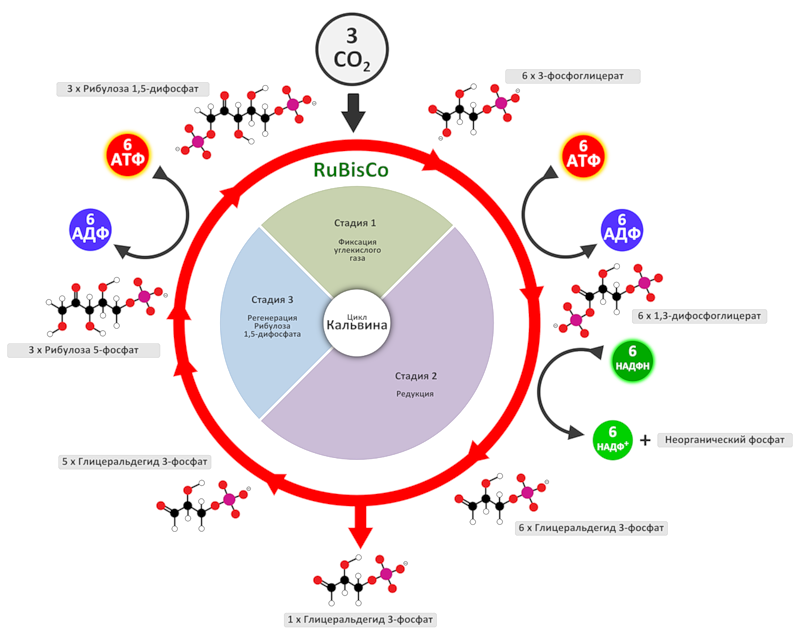
\includegraphics[width=0.6\linewidth]{pictures/calvin}
\caption{Схема ациклического пути фотосинтеза}
\label{calvin}
\end{figure}
%%%%%%%%%%%%%%%%%%%%%%%%%%%%%%%%%%%%%%%%%%%%%%%%%%%%%%%%%%%%%%%%%%%%%%%%%%%%%%%%%%%%%%%%%% 


\begin{enumerate}

\item Карбоксилирование. На этом этапе, молекула $CO_{2}$ соединяется с пятиуглеродным сахаром \termin{рибулозо-1,5-бифосфатом}. В результате образуется две молекул \termin{3-фосфоглицериновой кислоты} (ФГК). Реакцию карбоксилирования катализирует \hyperlink{enzimes}{фермент} \termin{рибулобисфосфаткарбоксилаза} (Сокращенно РуБисКо). \note{Молекулярная масса этого фермента очень высока -- 540 кДа, он состоит из 8 больших (55 кДа) и 8 малых (13 кДа), кодируемых как геномом хлоропластов, так и ядерным геномом. Этот этап фотосинтеза наиболее важен для биосферы. РУБИСКО является наиболее распространенным ферментом в биосфере -- его количество на нашей планете составляет около 10 млн. т, или около 2 кг на каждого жителя Земли. С участием этого фермента фотосинтезирующие организмы Земли ежегодно ассимилируют около 200 млн т $CO_{2}$ , превращая его в органические соединения, используемые всеми живыми организмами планеты \cite{medvedev_2012}}

\item Восстановление 3-\gls{fgac}. На этой стадии \gls{fgac} восстанавливается до 3-фосфоглицеринового альдегида \remember{Путь превращения 3-\gls{fgac} -- это центральное звено темновой стадии }. Этот Процесс идет в два этапа. 

\begin{enumerate}

\item Вначале, под действием фермента фосфоглицераткиназы от молекулы \gls{atp} на 3-\gls{fgac} переносится еще одна фосфатная группа и образуется 1,3-дифосфоглицериновая кислота (1,3-ФГК) с макроэргической связью \cite{medvedev_2012}. 

\item Затем происходит восстановление 1,3-\gls{fgac} в 3-фосфоглицериновый альдегид (3-ФГА) за счет \gls{nadfh2}. Этот процесс катализируется ферментом \termin{триозофосфатдегидрогеназой}. \note{Восстановление 1,3-\gls{fgac} до 3-\gls{fgal} — единственный восстановительный процесс цикла Кальвина, в котором используется \gls{nadfh2}, образуемый в фотохимических реакциях фотосинтеза. Последующие процессы цикла Кальвина необходимы для того, чтобы регенерировать (синтезировать) первичный акцептор $CO_{2}$ — рибулозо-1,5-бисфосфат для того, чтобы он вновь участвовал в фиксации $CO_{2}$.}

\end{enumerate}

\item Регенерация акцептора углекислого газа. На этой стадии, в результате внутримолекулярные перегруппировки фосфорсодержащих сахаров, 5 молекул трехуглеродного соединения \gls{fgal} превращаются в 3 молекулы пятиуглеродно сахара \termin{рибулозо-1,5-бифосфата}. На этом этапе цепь реакций цикла Кальвина замыкается.

\end{enumerate}


%1. Сначала из 3-ФГК с участием фермента фосфоглицераткиназы и АТФ образуется 1,3-дифосфоглицериновая кислота (1,3-ДФГК) с макроэргической связью. 
%2. Далее фермент триозофосфатдегидрогеназа с участием НАДФН+Н восстанавливает 1,3-ДФГК до 3-фосфоглицеринового альдегида (3-ФГА). Таким образом, в реакциях превращения 3-ФГК в 3-ФГА расходуются богатые энергией продукты световой фазы фотосинтеза: 2 молекулы НАДФН+Н и 2 молекулы АТФ.
%3. Дальнейшие реакции ВПФ-цикла направлены на превращение трехуглеродных соединений (3-ФГА и его изомера диоксиацетонфосфата (ДОАФ)) в пятиуглеродный акцептор СО2 – рибулозо-1,5-бисфосфат, а также на получение продуктов фотосинтеза (сахароза, крахмал). 
 

%В реакции превращения рибулозо-5-фосфата в рибулозо-1,5-бисфосфат расходуется еще одна молекула АТФ, образованная в результате фотофосфорилирования.
%Из реакций ВПФ-цикла для дальнейшего превращения в продукты фотосинтеза необходимо вывести молекулу фосфорсодержащего сахара. Такой молекулой с минимальным числом атомов углерода является 3-ФГА (или 3-ФГК). Поэтому для баланса цикла в него необходимо ввести три молекулы СО 2. 
%Тогда при полном обороте цикла из пяти молекул 3-ФГК можно получить в конечном итоге три молекулы рибулозо-1,5-бисфосфата. При этом на осуществление реакций требуется 6 молекул НАДФН+Н (если из цикла уходит 3-ФГА) и 9 молекул АТФ. Соотношение НАДФН+Н/АТФ, равное 2/3, должно обеспечивать световые реакции фотосинтеза.

\paragraph{Баланс веществ в цикле Кальвина}

\paragraph*{}Таки образом, в ходе реакций цикла Кальвина синтезируется шесть молекул \gls{fgal}, одна из которых выводится из цикла, а пять идут на регенерацию рибулезо-2-фосфата.  

\paragraph*{}Так как на синтез глюкозы необходимы 2 молекулы \gls{fgal}, образующиеся в результате двух оборотов цикла Кальвина, можно подсчитать, что на синтез одной молекулы глюкозы расходуется 12 молекул \gls{nadfh2} и 18 молекул \gls{atp}.

\subsubsection*{Фиксация углекислого газа в цикле Хэтча-Слэка-Карпилова}

\note{Основой для биохимических исследований фотосинтеза у С4-растений стали работы Коршака и его сотрудников (Гонолулу), в СССР – Ю.С. Карпилова и его сотрудников, в Австралии – Хэтча, Слэка и Джонсона.}

\paragraph*{}Растения, способные усваивать углекислый газ по C4 пути имеют некоторые характерные черты анатомического строения:

\begin{enumerate}
	\item Проводящие пучки листьев таких растений окружены двойным слоем зеленой ассимиляционной паренхимы, внешний слой которой состоит из клеток мезофилла, а внутренний из клеток обкладки пучка. 
	\item При этом клетки обкладки отличаются как структурно так и функционально:
	\begin{enumerate}
	
		\item \hyperlink{cell_plastids}{Хлоропласты} клеток обкладки содержат много зерен крахмала и не содержат гранн
		\item В хлоропластах клеток обкладки наблюдается низкая активность фотосистемы 2, в результате чего практически не происходит \hyperlink{photolisys}{фотолиза} воды и не выделяется кислород.
	
	\end{enumerate}	 
		
	\item В листе содержится много воздушных полостей
	
\end{enumerate}

\paragraph*{}Так же как и в случае цикла Кальвина, при образовании С4-соединений в цикле Хэтча-Слэка-Карпилова, расходуются продукты \hyperlink{light_stage}{световой фазы} фотосинтеза (\gls{atp} и \gls{nadfh2}), однако, C4-путь фиксации углерода заметно отличается от цикла Кальвина. Можно выделить следующие черты, отличающие С4-растения от С3-растений следующие: 

\begin{enumerate}

	\item Источником $CO_{2}$ для ВПФ-цикла служат С4-органические кислоты, а не $CO_{2}$ атмосферы; 
	\item Первоначально атмосферный углекислый газ соединяется с С3-соединением \gls{fep}, которое превращается в С4-соединение щавелево-уксусной кислоты (оксалоацетат), или ЩУК, с участием цитоплазматического фермента \gls{fep} – карбоксилазы; 
	\item У C4 растений реакции фиксации $CO_{2}$ пространственно разделены между двумя типами клеток. 
	\item При этом С4-соединения выполняют роль челноков, переносящих углерод и свободную энергию в клетки обкладки проводящих пучков, где локализованы ферменты ВПФ-цикла; 
	\item После декарбоксилирования образующиеся С3-соединения возвращаются в клетки, где локализованы соответствующие им карбоксилазы. 
	%\item Вторичное включение $CO_{2}$ в ВПФ-цикл с образованием сахарозы (клетки обкладки проводящих пучков).

\end{enumerate}


\note{В настоящее время составляет около 10000 видов однодольных и двудольных растений, среди которых такие сельскохозяйственно-значимые культуры как кукуруза, сорго, просо и сахарный тростник}

\paragraph*{}Появление C4-пути связано с тем, что \hyperlink{enzimes}{фермент} РуБисКо обладает высокой окислительной активностью, так как изначально был приспособлен для работы в условиях высокой концентрации углекислого газа. По этой причине работа этого фермента в условиях низкой концентрации углекислого газа малоэффективна. Карбоксилазы С3-соединений, в отличие от фермента Рубиско, не имеют оксигеназной активности и способны работать при крайне низких отношениях $CO_{2}/O_{2}$ в атмосфере. Таким образом, С4-путь позволяет увеличить эффективность как первичной фиксации углекислого газа, так и вторичной, связанной с ферментом Рубиско (за счет увеличения концентрации $CO_{2}$ и снижения концентрации $O_{2}$).

\paragraph*{}Дефицит углекислого газа может наблюдаться в условиях засушливого климата, когда устьица подолгу закрыты и, следовательно, поступление углекислого газа из атмосферы к ассимиляционному мезофиллу затруднено.

\remember{C4-путь ассимиляции углерода это приспособление к существованию растений в условиях низкой концентрации углекислого газа. Смысл C4-пути состоит в том, что углекислый газ изначально концентрируется в виде четырехуглеродных сахаров в клетках обкладки, а затем переправляется в клетки мезофилла. За счет этого в клетках мезофилла создается нужная для работы РуБисКо концентрация углекислого газа}

\subsubsection*{Первичные продукты фотосинтеза}

Первичными можно считать продукты фотосинтеза, образующиеся из промежуточных соединений ВПФ-цикла раньше конечных углеводов. 
К таким продуктам у хлореллы относятся аминокислоты 

\begin{enumerate}

\item аланин, 
\item серин, 
\item аспарагиновая кислота, 
\item глутаминовая кислота. 

\end{enumerate}

\paragraph*{}Аминокислоты, появившиеся в хлоропластах во время фотосинтеза, включаются в белок раньше и с большей эффективностью, чем аминокислоты, образованные в темновых реакциях превращения сахаров. 
На свету активируется синтез липидов, в который вовлекаются ДОАФ и двухуглеродные фрагменты, присутствующие в реакциях с участием транскетолаз.

\paragraph*{}Факторами, регулирующими пути усвоения $CO_{2}$ при фотосинтезе, являются 

\begin{enumerate}

\item физиологическое состояние растения, 
\item освещенность, 
\item водоснабжение,
\item минеральное питание, 
\item содержание $CO_{2}$. 
\item Отношение восстановленного \gls{nadfh2} к \gls{atp}. При недостатке \gls{atp} превращение 3-\gls{fgac} в 3-\gls{fgal} может быть затруднено и 3-\gls{fgac}будет направлена на образование \gls{fep}.

\end{enumerate}

\subsection*{Фотодыхание}

\paragraph*{}Фотодыхание – процесс поглощения кислорода и выделения $CO_{2}$ хлоропластами на свету. Точно измерить интенсивность фотодыхания трудно, так как при этом одновременно идут и фотосинтез и митохондриальное дыхание. 

\paragraph*{}Разветвление процессов фотосинтеза и фотодыхания происходит на уровне ключевого фермента ВПФ-цикл-Рубиско. Фермент проявляет свойства оксигеназы. Конечным продуктом фотодыхания, как и ВПФ-цикла, является молекула \gls{fgac}. Поэтому фотодыхание можно рассматривать как биохимический шунт, обеспечивающий работу цикла в условиях, когда фермент Рубиско функционирует при недостатке $CO_{2}$ или избытке кислорода.

\paragraph*{}В основе фотодыхания лежит гликолатный путь С3-растений. При этом, процесс фотодыхания имеет следующие особенности: 

\begin{enumerate}
	\item $CO_{2}$ образуется в реакции превращения двух молекул глицина в серин
	\item кислород расходуется как при образовании гликолата с участием фермента Рубиско, так и при окислении гликолата с участием гликолатоксидазы
	\item образуется свободный аммиак
	\item в гликолатном цикле расходуется энергия \gls{atp} и \gls{nadfh2}
	\item \gls{fgac} может расходоваться на синтез сахарозы и крахмала (гликогенолиз)
	\item Цикл основан на челночном переносе метаболитов между компартметами клетки – цитоплазмой, хлоропластами, митохондриями и пероксисомами
	
\end{enumerate}

\paragraph*{}Фотодыхание свойственно С3-растениям и эукариотическим водорослям.

\subsection*{Вопросы и задания для самоконтроля}

\begin{enumerate}
	\item По учебнику органической химии повторите суть реакции \hypertarget{eterefication}{этерефикеции}. Для каких классов химических веществ характерна эта реакция?

	\item Что такое \hyperlink{question_photo_unit}{фотосинтетическая единица}, фотосистема, реакционный центр?

	\item Какие особенности \hypertarget{question_bounds}{структуры} молекулы хлорофилла позволяют ей легко возбуждаться под действием солнечного света?

	\item Какие процессы световой стадии фотосинтеза являются \hypertarget{question_chem_phys}{фотофизическими}, а какие -- фотохимическими и почему?

	\item Объясните, в чем заключается \hypertarget{question_photocooperation}{согласованная} работа двух фотосистем при нециклическом фосфорилировании?
\end{enumerate}
	
	\section{Дыхание}
	
	%\note{Все живые организмы дышат, т. е. поглощают кислород и выделяют углекислый газ и воду. При этом происходит разложение органических веществ и выделение энергии, необходимой для жизни каждой клетки, всего растения.}

\subsection*{Общие сведения о процессе дыхания}

%Процесс превращения исходного органического вещества до более простых и затем до СО2 и Н2О требует большого числа различных ферментов.

\subsubsection*{Суммарное уравнение дыхания}

\begin{equation}
	 C_{6}H_{12}O_{6} + 6O_{2} = 6CO_{2} + 6H_{2}O.
	 \label{braezing_balance}
\end{equation}

\note{Данная формула характеризует начальный и конечный момент процесса \hypertarget{sect_breazing}{дыхания}. В действительности этот процесс многоступенчатый. Он состоит из целого ряда последовательно идущих окислительно-восстановительных реакций.}

%Итак, для дыхания нужно органическое вещество, включающее в себя запас потенциальной энергии, и кислород.

\subsubsection*{Субстраты дыхания}

\paragraph*{}В процессе дыхания окислению могут подвергаться большое количество разнообразных органических веществ, чаще всего это:

\begin{enumerate}

\item углеводы
\item белки 
\item жиры. 

\end{enumerate}

\paragraph*{}Типичным и наиболее выгодным для дыхания соединением, окисляемым в процессе дыхания, является глюкоза.  

\paragraph*{}По отношению объемов поглощенного организмом кислорода и выделенного углекислого газа, можно сделать вывод о химической природе используемого в процессе дыхания. Так, при окислении глюкозы, как следует из балансового уравнения \ref{braezing_balance} объемы выделенного при дыхании углекислого газа и поглощенного кислорода, должны быть равны. 

\remember{Отношение объема выделившегося углекислого газа к объему поглощенного кислорода $CO_{2}/O_{2}$ называется \hypertarget{breazing_index}{\gls{breazingIndex}}}

\paragraph*{}Если исходным дыхательным материалом является сахар, то этот коэффициент обычно равен 1.

\paragraph*{}В том случае, когда исходным материалом будут жиры или белки, на окисление которых нужно больше кислорода из воздуха, дыхательный коэффициент снизится до 0,7-0,8.

\note{Например, если исходным веществом будет стеариновая кислота, то процесс дыхания пойдет по суммарному уравнению:



$C_{18}H_{36}O_{2} + 26O_{2}  = 18CO_{2} + 18H_{2}O$



В данном случае, дыхательный коэффициент будет равен 18:26 = 0,69.}

\paragraph*{}Если же исходным веществом будут соединения, богатые кислородом, то для их окисления потребуется меньше кислорода воздуха, и дыхательный коэффициент повысится.

\note{Так, при дыхании за счет щавелевой кислоты уравнение примет следующий вид:



$2C_{2}O_{4}H_{2} + O_{2} = 4CO_{2} + 2H_{2}O$



Дыхательный коэффициент будет равен 4/1 = 4. }

\paragraph*{}Чем выше дыхательный коэффициент, тем ниже тепловой эффект, и наоборот. Поэтому жиры и белки отличаются более высоким тепловым эквивалентом.
%Сравнивать дыхание у разных органов растения можно по выделению СО2 на 1 г сухого вещества в единицу времени при определенной температуре, т. е. по интенсивности дыхательного процесса.

\paragraph*{}Определению дыхательного коэффициента прорастающих семян посвящена одна из \hyperlink{breazing_index_lab}{лабораторных работ}.

\note{Установлено, что растущие органы дышат интенсивнее нерастущих. Прорастающие семена, цветки, плоды, мицелий грибов дышат более интенсивно, чем другие органы.} 

\paragraph*{}Фотосинтез и дыхание можно рассматривать как два противоположных процесса. Если в растении оба процесса будут протекать с одинаковой интенсивностью, то накопления органического вещества не будет. В пасмурную и холодную погоду такое явление может произойти. 

\paragraph*{}Интенсивность света, при которой количество создаваемого органического вещества при фотосинтезе равно трате его на дыхание, называется компенсационной точкой. Для световых и теневых растений компенсационная точка будет различная.

\subsection*{Факторы, влияющие на интенсивность дыхания}

\paragraph*{}На интенсивность дыхания влияют следующие факторы

\begin{enumerate}

\item температура, 
\item влажность, 
\item наличие ядовитых веществ и физических агентов, 
\item содержание кислорода в воздухе.

\end{enumerate}

\subsubsection*{Влияние температуры воздуха и почвы}


\paragraph*{}Влияние температуры на жизненные процессы подчиняется правилу Вант-Гоффа, согласно которому, при повышении температуры на каждые 10 \celsius скорость процесса удваивается. Это ускорение носит название температурного коэффициента. Он равен примерно 2. \gls{VanGoffRule} действует в \hyperlink{question_van_goff}{пределах} до 40 \celsius. 

\paragraph*{}Дыхание у растений происходит в довольно широких границах температур.

\note{У зимующих растений дыхание можно обнаружить и при 20-25 \celsius мороза}

\paragraph*{}Оптимальная температура для дыхания прорастающих семян 30 и 40 \celsius. При температуре 50 \celsius дыхание прекращается, так как белки цитоплазмы свертываются.

\subsubsection*{Насыщенность клеток водой}

\paragraph*{}Вода необходима для набухания коллоидов цитоплазмы. 
Сухие семяна выделят очень незначительное количество углекислого газ. Во влажных семенах выделение $CO_{2}$ увеличивается в 10000 раз. Поэтому хранение зерна, имеющего влажность свыше 12-14 \%, приводит к потере органического вещества и всхожести. 
Зерно темнеет и портится (<<сгорает>>).

\note{Например, семена ячменя (с 10-12 \% гигроскопической воды) выделяют за сутки ничтожное количество углекислого газа (0,3-0,4 мг). При повышении содержания воды до 33 \% (почти полном набухании) количество выделенного $CO_{2}$ достигает 2 г)}

\subsubsection*{Наличие ядовитых веществ и физических агентов}

\paragraph*{}Такие вещества, как 

\begin{enumerate}

\item эфир
\item хлороформ 
\item нейтральные соли щелочных и щелочно-земельных металлов

\end{enumerate}
 
в больших дозах вызывают быстрое падение дыхания вследствие отравления растения. В малых дозах они действуют стимулирующее -- интенсивность дыхание повышается.

\subsubsection*{Влияние концентрации кислорода в воздухе}

\paragraph*{}Небольшие колебания в содержании кислорода в воздухе (20,95 \%) особого влияния на процесс дыхания не оказывают. Падение же его содержания до 1-2 \% приводит обычно к снижению интенсивности дыхания. 

\note{Недостаток кислорода возможен и внутри некоторых семян, имеющих плотную кожуру. Накопившийся в них углекислый газ действует на семена как анестезирующее средство (делающее их нечувствительными). Не теряя всхожести, такие семена могут длительное время находиться в почве, не прорастая (многие сорняки). В настоящее время $CO_{2}$ применяют для сохранения плодов и овощей.}

%Дыхание и брожение в современном изложении

%Процессы дыхания и брожения имеют очень сложные срединные звенья, связанные с образованием многих промежуточных продуктов. Благодаря этому указанные процессы тесно связаны с общим обменом веществ в растении.
%В результате более детального исследования спиртового брожения было выяснено, что оно является по существу первой фазой дыхания. Лишь вторая фаза, после образования пировиноградной кислоты, будет у обоих процессов различна. 
 
%Далее при дыхании происходит ступенчатое превращение последней в присутствии кислорода в СО2 и Н2О с выделением (в целом) 686 ккал энергии. Оно называется циклом Кребса. 

\subsection*{Гликолиз}

%При брожении пировиноградная кислота в отсутствие кислорода постепенно превращается в спирт и СО2 с выделением 24 ккал.

\termin{\hypertarget{glycolysis}{\gls{glycolisys}}} -- это процесс распада сахаров, который происходит с образованием глюкоза-6-фосфата и заканчивается образованием прировиноградной кислоты.

\paragraph*{}Гликолиз является первой стадией как брожения так и аэробного дыхания.

\paragraph*{}Реакции гликолиза происходят в \hyperlink{protoplast}{цитоплазме} и в \hyperlink{plastides}{хлоропластах}. Последовательность реакций гликолиза можно разделить на три стадии:

\begin{enumerate}
	\item Подготовительный этап. В ходе данного этапа образуется фруктозо-1,6-бисфосфат, который затем расщепляется на две фосфотриозы: \gls{fgal} и \termin{фосфодиоксиацетон}.
	\item Первое \hypertarget{substratickFosforolysis}{субстратное фосфорилирование}. На этом этапе \gls{fgal} сначала окисляется с образованием \gls{nadh} и 1,3-бисфосфоглицериновой кислоты (1,3-\gls{fgac}). Затем 1,3-\gls{fgac} дефосфорилируется с образованием \gls{atp} и 3-\gls{fgac}.
	\item Второе субстратное фосфорилирование, В ходе этого этапа происходит образование еще одной молекулы \gls{atp} при переносе фосфатной группы с фосфоенолпировиноградной кислоты \gls{fep} на АДФ.

\end{enumerate}

%АТФ в растении образуется не только в хлоропластах, о чем было сказано ранее, но и в митохондриях, при наличии кислорода и окислительных ферментов. Такой способ образования АТФ называется окислительным фосфорилированием (в отличие от фотосинтетического фосфорилирования). Энергию для реакции АДФ + Н3РО4 = АТФ + Н2О растение получает в результате процесса дыхания, а не солнца. При переходе АТФ – АДФ растение получает 8— 10 ккал, которые используются для эндотермических (требующих затраты энергии) реакций.
%Чтобы яснее представить сложность гликолиза, рассмотрим ход последовательных превращений глюкозы до \gls{pva}:

\paragraph*{}Обобщив вышесказанное, можно составить следующую цепь превращений, происходящих в ходе \gls{glycolisys}а:

Глюкоза $\rightarrow$ Глюкозо-6-фосфат $\rightarrow$ Фруктозо-1,6-дифосфат $\rightarrow$ \gls{fgal} $\rightarrow$ Дифосфоглицериновая кислота $\rightarrow$ 3-\gls{fgac} $\rightarrow$ 2-Фосфоглицериновая кислота $\rightarrow$ Фосфоэнолпировиноградная кислота $\rightarrow$ Энолпировиноградная кислота $\rightarrow$ \gls{pva}.

\subsubsection*{Энергетика гликолиза}

\paragraph*{}На образование фруктоза-1,6-бифосфата тратится 2 молекулы \gls{atp}. В результате же двух субстратных фосфорелирований образуется 4 молекулы \gls{atp}. Таким образом, <<чистый>> энергетический выход гликолиза -- 2 молекулы \gls{atp} (4-2=2). Кроме того, в результате гликолиза образуется 2 молекулы \gls{nadh}. 

\paragraph*{}Учитывая то, что в аэробных условиях окисление \gls{nadh} приведет к образованию еще 6-и молекул \gls{atp}, энергетический выход гликолиза в аэробных условиях будет 8 молекул \gls{atp} (2+6=8).

\paragraph*{}В дальнейшем, образовавшаяся пировиноградная кислота в процессе дыхания претерпевает превращения в ходе реакций цикла Кребса.

\subsubsection*{Отличительные особенности гликолиза в клетках растений}

\paragraph*{}В отличии от клеток животных, процесс \gls{glycolisys}а в растительной клетке имеет следующие особенности \cite{medvedev_2012}:

\begin{enumerate}

\item У растений \gls{glycolisys} может идти не только в цитоплазме, но и в хлоропластах
\item В отличии от животных, исходным соединением для гликолиза является не глюкоза а сахароза.
\item Конечным продуктом гликолиза может быть не только \gls{pva}, но и малат

\end{enumerate}

\subsection*{Цикл Кребса}  

\paragraph*{}\hypertarget{krebs_cycle}{Цикл Кребса}\footnote{Нередко цикл Кребса называют лимонно-кислым циклом или циклом трикарбоновых кислот}, является основным этапом процесса дыхания. Этот процесс практически универсален, является главным путем окисления остатков уксусной кислоты у всех живых организмов. Цикл Кребса происходит в матриксе \hyperlink{митохондрий}.     
  
%В ходе видоизменения одних кислот в другие выделяются СО2 и Н2О. Углерод окисляется кислородом воды, а не кислородом из внешней среды. Последний же окисляет выделяющийся водород и образует воду.


\paragraph*{}Цикл Кребса (\ris \ref{krebs_cycle}) включает в себя 8 последовательных реакций и состоит из двух стадий.

%%%%%%%%%%%%%%%%%%%%%%%%%%%%%%%%%%%%%%%%%%%%%%%%%%%%%%%%%%%%%%%%%%%%%%%%%%%%%%%%%%%%%%%%%%%%%%%%%%%%%%%%%%% 
\begin{figure}
  \centering
       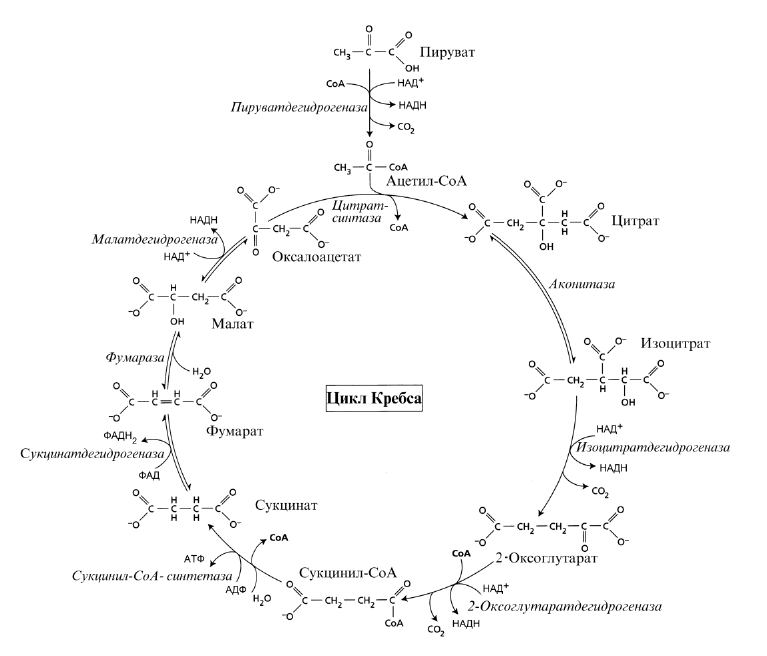
\includegraphics[width=1\linewidth]{pictures/krebs_cycle}
\caption{Схема реакций цикла Кребса}
\paragraph*{}Приведена из \cite{medvedev_2012}
\label{krebs_cycle}
\end{figure}
%%%%%%%%%%%%%%%%%%%%%%%%%%%%%%%%%%%%%%%%%%%%%%%%%%%%%%%%%%%%%%%%%%%%%%%%%%%%%%%%%%%%%%%%%% 

\begin{enumerate}

\item В начале цикла от молекулы \gls{pva} отделяется одна молекула углекислого газа, а оставшийся фрагмент, в виде ацетильного остатка соединяется с коэнзимом А. Отщепление углекислого газа от пировиноградной кислоты носит название \termin{декарбоксилирование}. Образовавшийся при этом \gls{acetylCoensimA},является ключевым веществом, входящим в собственно цикл Кребса\footnote{\gls{acetylCoensimA} может образовываться и в результате ряда других химических реакций}

\item \gls{acetylCoensimA} включается в цикл Кребса путем присоединения его к щавелевоуксусной кислоте (четырехуглеродному соединению, дикарбоновой кислоте), в результате чего образуется лимонная кислота (шестиуглеродное соединение, трикарбоновая кислота). После образования лимонной кислоты через ряд промежуточных соединений происходит образование 
щавелевоуксусной кислоты, при этом выделяется две молекулы $CO_{2}$ и 8$H^{+}$.

\end{enumerate}

\paragraph*{}Ниже перечислена последовательность реакций цикла Кребса и \hyperlink{enzimes}{ферменты} участвующие в этих реакциях:

\begin{enumerate}

\item Aцетильная группа \gls{acetylCoensimA} конденсируется с оксалоацетатом, в результате чего образуется лимонная кислота. Реакция катализируется \termin{цитрат-синтазой}

\item Лимонная кислота подвергается дегидратированию с образованием \termin{цис-аконитовой кислоты}, затем, к цис-аконитовой кислоте присоединяется молекула воды. При этом цис-аконитовая ксилота переходит в изолимонную кислоту (изоцитрат). Катализирует эти обратимые реакции фермент \termin{аконитатгидратаза}. В результате происходит взаимоперемещение Н и ОН в молекуле цитрата:

\item Изолимонная кислота дегидрируется при участии фермента \termin{НАД-зависимой изо-цитратдегидрогеназы.}

\item В результате окислительного декарбоксилирования $\alpha$-кетоглутаровой кислоты образуется высокоэнергетическое соединение сукцинил-КоА. В данной реакции принимают участие 5 \gls{coenzim}ов: ТПФ, амид липоевой кислоты, HS-KoA, ФАД и НАД+.

\item Сукцинат дегидрируется в фумаровую кислоту. Окисление сукцината катализируется сукцинатдегидрогеназой, в молекуле которой с белком прочно (ковалентно) связан \gls{coenzim} ФАД. \note{В свою очередь сукцинатдегидрогеназа прочно связана с внутренней ми-тохондриальной мембраной}

\item Фумаровая кислота гидратируется, продуктом реакции является яблочная кислота (малат). Реакция осуществляется под влиянием фермента \termin{фумаратгидратазы} (фумаразы).

\item Под влиянием митохондриальной НАД-зависимой малатдегидрогеназы происходит окисление L-малата в оксалоацетат

\end{enumerate}

\paragraph*{}Через образование \gls{pva} и ряда других органических кислот в процесс дыхания поступают также продукты разложения белков -- аминокислоты. При этом углеродные скелеты аминокислот подвергаются окислительному расщеплению на фрагменты. 

\note{Такие аминокислоты как аланин, цистеин, глицин, серин и треонин образуют \gls{acetylCoensimA} через пировиноградную кислоту, а лейцин, лизин, фенилаланин, тирозин и триптофан образуют \gls{acetylCoensimA} через ацетоацетилКоА. Пролин, гистидин, аргинин, глутамин и клутаминовая кислота включаются в цикл Кребса через a-кетоглутаровую кислоту, метионин, изолейцин и валин - через янтарную кислоту, фенилаланин и тирозин - через фумаровую кислоту, аспарагин и аспарагиновая кислота - через щавелевоуксусную кислоту.}

\remember{Физиологический смысл цикла Кребса состоит в том, что именно здесь происходит разложение органического вещества (\gls{pva}) до неорганических веществ (углекислого газа и ионов водорода), при этом образуется большое количество энергии в виде молекул \gls{atp}.}

\subsubsection*{Энергетика цикла Кребса}

\paragraph*{}Таким образом, одна молекула \gls{nadh} образуется при окислительном декарбоксилировании пирувата в\gls{acetylCoensimA}. При участии данной молекулы позже образуются 3 молекулы \gls{atp} 

\paragraph*{}При расщеплении одной молекулы глюкозы образуется 2 молекулы пировиноградной кислоты, а при окислении их до 2 молекул \gls{acetylCoensimA} и последующих 2 оборотов цикла Кребса синтезируется еще 30 молекул \gls{atp}. 

\paragraph*{}Если учесть, что 8 молекул \gls{atp}, образующихся при аэробном \hyperlink{glycolysis}{гликолизе}, то, суммарно, при расщеплении в тканях одной молекулы глюкозы по уравнению \ref{braezing_balance} синтезируется 38 молекул \gls{atp}. 



\subsubsection*{Значение цикла Кребса}

\begin{enumerate}

\item \gls{acetylCoensimA} служит исходным продуктом для синтеза жирных кислот, для некоторых гормонов, терпенов, изопреноидов и стероидов.
\item Промежуточные продукты цикла Кребса являются <<сырьем>> для синтеза аминокислот, которые могут быть использованы растением в обмене веществ. Так некоторые кислоты (фумаровая, яблочная и др.), при присоединении к ним аминогруппы преобразуются в аминокислоты. Важную роль в этом процессе играют реакции трансаминирования, при этом аминогруппы большинства аминокислот переносятся на пировиноградную, щавелевоуксусную или a-кетоглутаровую кислоты.

\end{enumerate}

\subsection*{Гликооксалатный путь}

\subsection*{Вопросы и задания для самоконтроля}

\begin{enumerate}

\item В чем состоит значение процесса дыхания в \gls{metabolism}е клетки? 
\item Каково суммарное уравнение реакций аэробного дыхания? 
\item Повторите особенности организации белковой молекулы. Почему, на ваш взгляд, интенсивность дыхания резко \hypertarget{question_van_goff}{падает} при температуре выше 50 \celsius.
\item Что такое окислительное фосфорилирование? 
\item В чем заключается роль гликолиза в \gls{metabolism}е клетки? 
\item Какие вещества поступают в цикл Кребса а какие выходят из него?
\item В чем заключается значение цикла Кребса для \gls{metabolism}а клетки?
\item В чем заключается сходство и различие между анаэробным дыханием в растительной клетки и спиртовым брожением?
\item Как происходят масляно-кислое и молочно-кислое брожения? У каких организмов происходит брожение такого типа?

\end{enumerate}

	
	\section{Минеральное питание растений}
	
	\subsection*{Поглощение веществ}

\paragraph*{}В процессе жизнедеятельности, растение поглощает из окружающей среды вещества, включающие в себя различные химические элементы. При этом, надо понимать, что значительная часть этих химических элементов необходимы растению для нормальной жизнедеятельности и не могут быть заменены на какие либо \hyperlink{libihBarell}{другие}. Такие, незаменимые химические элементы называются \gls{nutrientElements}. А соединения, в состав которых входят питательные элементы носят название \gls{nutrients}. Для растения питательными веществами служат минеральные соли, содержащиеся в почве.

\paragraph*{}\gls{nutrientElements} могут содержаться в почве в следующих формах: 

\begin{enumerate}

\item В недоступной для растения форме

	\begin{enumerate}

		\item В виде прочно фиксированных в различных минералах веществ; \note{например, ионы $K^{+}$ и $NH^{+}_{4}$ в некоторых глинистых минералах \cite{malinowsky_2004}}
		\item В виде труднорастворимых неорганических солей; \note{например различные сульфаты, фосфаты, карбонаты}

	\end{enumerate}
	
\item В доступной для растения форме

	\begin{enumerate}

		\item В виде адсорбированных на поверхности коллоидов, доступных для растений благодаря \hyperlink{contact_exchanging}{ионному обмену};
		\item В виде растворенных в воде и поэтому легко доступных для растений;

	\end{enumerate}

\end{enumerate}

\paragraph*{}Поглощаемые растением ионы поступают в клетки \hyperlink{question_rizoderma}{ризодермы} следующими путями:

\begin{enumerate}
	\item Непосредственно из почвенного раствора
	\item Благодаря контактному обмену $H^{+}$, $HCO^{-}_{3}$ и анионов органических кислот на ионы минеральных веществ почвенных частиц.
\end{enumerate} 

\subsubsection*{Поглощение веществ путем контактного обмена}

\paragraph*{}\note{Обменные катионы и анионы -- один из важнейших источников питания для растений}

\paragraph*{}При \hypertarget{contact_exchanging}{контактном обмене}, растение обменивает катионы и анионы, находящиеся на частицах почвы на ионы, адсорбированные на поверхности клеток корня. 

\paragraph*{}Путем контактного обмена может происходить поступление как катионов, так и анионов. Так, при поглощении катионов  $K^{+}$, $Ca^{2+}$, $Na^{+}$ растение обменивает их на \gls{proton}ы $H^{+}$. Анионы $NO^{-}_{3}$, $PO^{3-}_{4}$ поступают в корень в обмен на гидрокарбонат-ионы $HCO^{-}_{3}$ или анионы органических кислот. 

\paragraph*{}Контактный обмен ионов между \hyperlink{cell_wall}{клеточными стенками} клеток ризодермы и частицами почвы осуществляется без перехода ионов в почвенный раствор. Необходимый для этого тесный контакт между частицами почвы и клетками ризодермы обеспечивается благодаря следующим механизмам:

\begin{enumerate}
	\item Выделению слизи корневыми волосками
	\item Отсутствию у ризодермы кутикулы и других защитных покровов
\end{enumerate}
 
%Так как адсорбированные ионы находятся в постоянном колебательном движении и занимают определенный объем - сферу колебаний, при тесном контакте поверхностей сферы колебаний двух ближайших адсорбированных ионов могут перекрываться, в результате чего осуществляется ионный обмен. 
%Выделяя различные вещества (углекислый газ, аминокислоты, сахара и другие), корень растения изменяет состояние питательных веществ в прикорневой зоне непосредственно, например, путем выделения СО2 (СО2 + Н2О Н+ + НСО-3: повышение растворимости фосфатов и карбонатов) и косвенно, создавая благоприятные условия для ризосферы, которая играет большую роль в превращении почвенных минералов.

\paragraph*{}В целом, можно отметить следующие особенности поглощения растением минеральных веществ: 

\begin{enumerate}
	\item Количество минеральных веществ, поступивших в растение и накапливающихся в нем, не \hyperlink{what_is_transport_type}{пропорционально} количеству прошедшей через растение воды.
	\item Из очень разбавленных растворов соли поглощаются быстрее, чем вода.
	\item Из концентрированных растворов в растение быстрее поступает вода.
	\item Минеральные соли и вода поступают в растение относительно независимо друг от друга и с помощью различных механизмов.
\end{enumerate}

\subsubsection*{Этапы поглощения веществ}

\paragraph*{}Путь иона из почвенного раствора в органеллы клетки можно представить как последовательность следующих событий:

\begin{enumerate}

	\item Поступление ионов из почвенного раствора или из свободного пространства соседней клетки в свободное пространство \hyperlink{cell_wall}{клеточной стенки} ризодермы;
	\item Транспорт ионов через \hyperlink{plasmolema}{цитоплазмотическую мембрану} клетки в цитоплазму.
	\item Транспорт ионов в различные органеллы клетки через их мембраны. 

\end{enumerate}

\paragraph*{}Непосредственно через саму \hyperlink{plasmolema}{цитоплазматическую мембрану} ионы и \hyperlink{polarMolecula}{полярные молекулы} проникнуть не могут. Это связанно с тем, что:

\begin{enumerate}

	\item Внутренняя часть двойного липидного слоя мембраны гидрофобна и через нее заряженные частицы проникнуть не способны;
	\item Внешняя сторона цитоплазматической мембраны, в свою очередь, имеет электрический заряд. Так, поверхность \hyperlink{plasmolema}{плазмалеммы} заряжена отрицательно а поверхность \hyperlink{cell_vakuol}{тонопласта} -- положительно. По этой причине поверхность мембраны будет отталкивать одноименно заряженные ионы;
	\item Находящиеся в растворе ионы окружены гидратными оболочками, увеличивающими их размер.
	\item Концентрация веществ в клетке больше, чем в свободном пространстве, т.е. вещество должно двигаться против градиента концентрации.  

\end{enumerate}

\paragraph*{}Для того, чтобы растворенные в воде вещества смогли пройти через мембрану клетки в ней есть поры, образованные специальными \hyperlink{proteins}{белками}. 

\subsubsection*{Механизмы транспорта}

\paragraph*{}Различные механизмы транспорта веществ через мембрану можно разделить на следующие типы:

\begin{enumerate}

\item \gls{passiveTranspotr} -- это транспорт через мембрану без затраты энергии (в виде молекул \gls{atp}). При пассивном транспорте движение ионов происходит по градиенту электрохимического потенциала (\ris \ref{celltransport}). Основным механизмом пассивного транспорта является \gls{diffusion}.
	
\item \gls{activeTranspotr} -- это транспорт, идущий против электрохимического потенциала с затратой энергии (в виде молекул \gls{atp}), выделяющейся в процессе \gls{metabolism}а (\ris \ref{celltransport}). Основными механизмами активного транспорта являются:
	
	\begin{enumerate}
	
		\item Везикулярный транспорт, включающий \Gls{endocytosis}, экзоцитоз
		\item Молекулярный транспорт, происходящий через мембранные транспортные белки (белки-переносчики и каналообразующие белки).
	
	\end{enumerate}

\end{enumerate}

%%%%%%%%%%%%%%%%%%%%%%%%%%%%%%%%%%%%%%%%%%%%%%%%%%%%%%%%%%%%%%%%%%%%%%%%%%%%%%%%%%%%%%%%%%%%%%%%%%%%%%%%%%% 
\begin{figure}[h!]
  \centering
       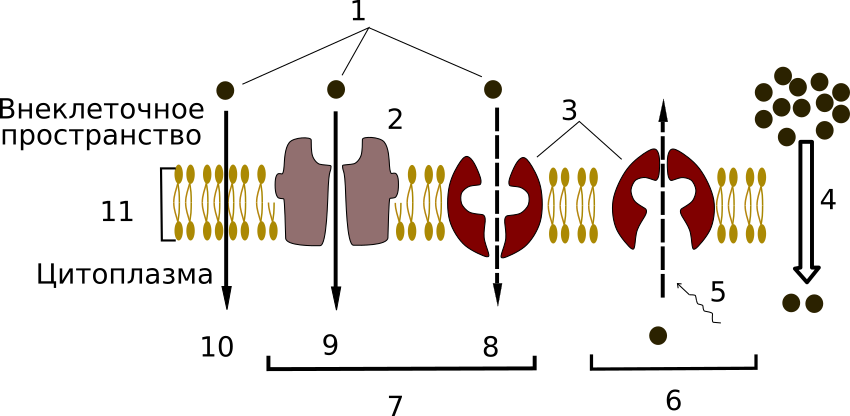
\includegraphics[width=0.7\linewidth]{pictures/celltransport}
\caption{Активный и пассивный транспорт вещество через цитоплазматическуцю мембрану}


\paragraph*{}1. Транспортируемая молекула; 2. Каналобразующий белок; 3. Белок переносчик; 4. Электрохимический градиент; 5. Энергия; 6. \gls{activeTranspotr}; 7. \gls{passiveTranspotr}; 8. \gls{diffusion} с помощью белка-переносчика; 9. \gls{diffusion} через канал; 10. Простая диффузия 11. Липидный слой. 

\paragraph*{}Рисунок приведен согласно Альбертсу Б \cite{alberts_2013}

\label{celltransport}
\end{figure}
%%%%%%%%%%%%%%%%%%%%%%%%%%%%%%%%%%%%%%%%%%%%%%%%%%%%%%%%%%%%%%%%%%%%%%%%%%%%%%%%%%%%%%%%%% 

\paragraph*{Пассивный транспорт}

\paragraph*{}Один из важнейших видов пассивного транспорта через мембраны -- это диффузия. \hypertarget{diffusion}{\gls{diffusion}} -- это самопроизвольное проникновение одного вещества в другое при их соприкосновении. Движение вещества путем диффузии происходит по градиенту концентрации; 

\paragraph*{}Путем диффузии в свободное пространство клеточной стенки поступают:

\begin{enumerate}
	\item вещества, растворимые в жирах
	\item $O_{2}$, $CO_{2}$
	\item этанол
\end{enumerate}

\paragraph*{}Через цитоплазматическую мембрану эти вещества попадают через специальные белки-\gls{porins}
 
%Закон диффузии: молекулы газа или растворенного вещества двигаются туда, где их меньше, т.е. по градиенту концентрации.

\paragraph*{}Белки-\gls{porins} (\ris \ref{porin}) -- образуют в липидном бислое мембраны <<поры>>, заполненные водой. Внутренняя поверхность этих белков гидрофильна, что позволяет проходить через нее молекулам воды и ионам. Внешняя же часть белка гидрофобна, что позволяет ему закрепится в липидном слое мембраны. Поры, образованные белками, могут открываться на короткое время и закрываться. Белковые каналы плазмалеммы обладают избирательностью, т.е. через них могут проходить ионы только определенного вида и размера.

%%%%%%%%%%%%%%%%%%%%%%%%%%%%%%%%%%%%%%%%%%%%%%%%%%%%%%%%%%%%%%%%%%%%%%%%%%%%%%%%%%%%%%%%%%%%%%%%%%%%%%%%%%% 
\begin{figure}[h!]
  \centering
       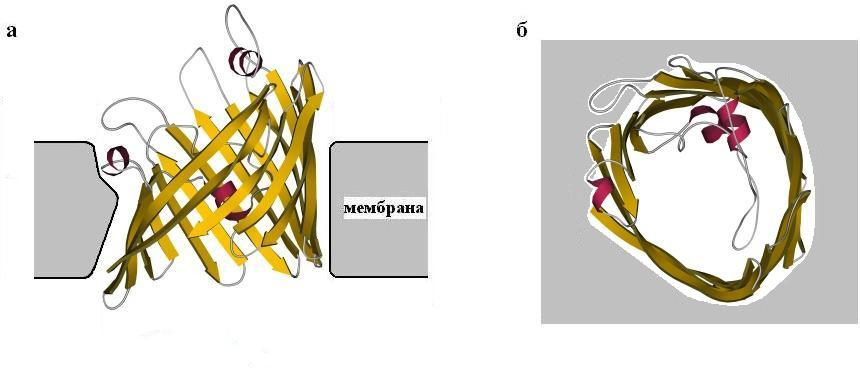
\includegraphics[width=0.5\linewidth]{pictures/porin}
\caption{Структура белка-порина}
\label{porin}
\end{figure}
%%%%%%%%%%%%%%%%%%%%%%%%%%%%%%%%%%%%%%%%%%%%%%%%%%%%%%%%%%%%%%%%%%%%%%%%%%%%%%%%%%%%%%%%%% 

\note{Через каналы, образованные белками, ионы транспортируются со скоростью 106 ионов в сек, т.е. в 1000 раз быстрее, чем с помощью белка-переносчика. Транспорт через каналы является всегда пассивным \cite{malinowsky_2004}}

\paragraph*{Активный транспорт}

\paragraph*{}Мембранные транспортные белки переносят маленькие водорастворимые молекулы (сахара, аминокислоты, нуклеотиды и др.)

\paragraph*{}\remember{Белки-переносчики переносят растворенные вещества через цитоплазматическую мембрану, изменяя свою форму, при этом участки белка, с которыми связывается ион, открываются то с одной, то с другой стороны мембраны}

\paragraph*{}У высших растений большое значение имеет деятельность такого белка переносчика, как протонная помпа. \gls{protonsPomp} -- это интегральный мембранный белок, осуществляющий перемещение \gls{proton}ов через мембрану.  Поскольку насос прокачивает протоны против градиента их концентрации, процесс идет с затратой \gls{atp} или \gls{nadfh2}. Вынос протонов на внешнюю сторону цитоплазматической мембраны сопровождается поступлением внутрь клетки катионов. Вместе с \gls{proton}ами в ту же сторону могут передвигаться и анионы.

\paragraph*{}\Gls{endocytosis} -- это активный способ поглощение макромолекул клеткой, сопровождающийся впячиванием участков мембраны и образованием везикул.  В ходе эндоцитоза происходит следующая последовательность событий (\ris \ref{endocytoze}):

\begin{enumerate}

	\item Поглощаемые клеткой макромолекулы адсорбируются на поверхности клеточной мембраны (\ris \ref{endocytoze} I);  
	\item Небольшой участок мембраны впячивается, окружая транспортируемое вещество (\ris \ref{endocytoze} II);
	\item В результате смыкания краев впячивания мембраны, образуя внутриклеточный пузырек -- \gls{vesicula} III;
	\item \gls{vesicula} отделяется от мембраны (например, плазмалеммы) и передвигается в цитозоле (\ris \ref{endocytoze} IV); 
	\item \gls{vesicula} соединяется с лизосомой, \hyperlink{enzimes}{ферменты} которой или разрушают мембрану везикулы или разрушают само вещество находящиеся внутри везикулы (\ris \ref{endocytoze} V); 
	\item Образовавшиеся мелкие фрагменты содержимого везикулы проходят через мембрану везикулы в цитозоль

\end{enumerate}

%%%%%%%%%%%%%%%%%%%%%%%%%%%%%%%%%%%%%%%%%%%%%%%%%%%%%%%%%%%%%%%%%%%%%%%%%%%%%%%%%%%%%%%%%%%%%%%%%%%%%%%%%%% 
\begin{figure}[h!]
  \centering
       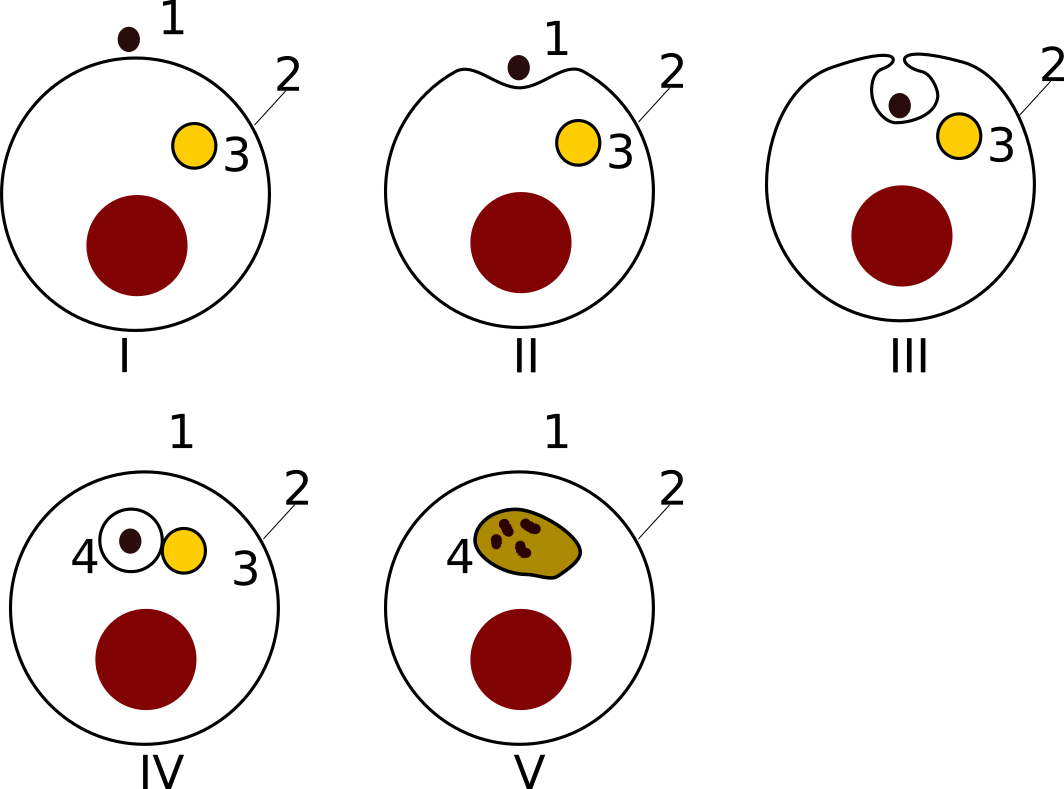
\includegraphics[width=0.7\linewidth]{pictures/endocytoze}
\caption{Стадии эндоцитоза}
\label{endocytoze}
\end{figure}
%%%%%%%%%%%%%%%%%%%%%%%%%%%%%%%%%%%%%%%%%%%%%%%%%%%%%%%%%%%%%%%%%%%%%%%%%%%%%%%%%%%%%%%%%% 

\subsection*{Влияние факторов окружающей среды на активность поглощения минеральных веществ}

\subsubsection*{Температура}

\paragraph*{}При температуре, близкой к 0 \celsius, поглощение солей идет медленно, затем, в пределах до 40 \celsius, оно усиливается. Увеличение интенсивности поглощения солей идет согласно правилу Ван-Гоффа -- увеличение температуры на 10 \celsius может вызвать возрастание поглощения в 2-3 раза.

\subsubsection*{Свет}

\paragraph*{}Свет может оказывать на интенсивность поглощения солей как прямое, так и косвенное влияние.

\begin{enumerate}
	\item Прямое влияние заключается в том, что в темноте поглощение солей замедляется и постепенно прекращается, а на свету -- ускоряется. \note{При этом, на прямое влияние света указывает быстрота с которой изменяется скорость поглощения ионов растением}
	\item Косвенное влияние заключается в том, что на свету, в процессе \hyperlink{photosyntesis}{фотосинтеза}, образуются \hyperlink{sect_glycosids}{углеводы}, которые необходимы для \hyperlink{sect_breazing}{дыхания} и образования \gls{atp}, энергия которой используется на поступление веществ. 
\end{enumerate}

\subsubsection*{Концентрация кислорода}

\paragraph*{}При уменьшении содержания кислорода до 2—3\% интенсивность поступления солей остается на одном уровне. Лишь снижение концентрации кислорода ниже 3\% вызывает падение поглощения примерно в два раза. 

%\paragraph*{}Поглощение одного иона зависит от присутствия других ионов. Так, в присутствии легко поглощаемого аниона катионы той же соли поступают быстрее. Ионы с одинаковым зарядом обычно конкурируют между собой.

\subsubsection*{Влияние внутренних факторов на поступление солей} 

\paragraph*{}На интенсивность поступления минеральных веществ в корень оказывают влияние такие внутренние факторы, как:

\begin{enumerate}
	\item Интенсивность \hyperlink{sect_breazing}{дыхания}. При этом можно выделить следующие направления влияния
	\begin{enumerate}
		\item В процессе \hyperlink{sect_breazing}{дыхания} выделяется углекислый газ, который в воде образует угольную кислоту. Адсорбируясь на поверхности корня, эти ионы служат обменным фондом для поступающих катионов и анионов.
%		\item В процессе переноса ионов через мембрану участвуют специфические ё	ся в зависимости от интенсивности дыхательного процесса.
		\item В процессе дыхания накапливается энергия (в форме макроэргических связей \gls{atp}), необходимая для активного поступления ионов
	\end{enumerate}	
	\item Наличие токсинов-ингибиторов дыхания. Ингибиторы процесса \hyperlink{sect_breazing}{дыхания} (в частности, цианистый калий) резко тормозят поступление солей. 
	
\end{enumerate}

\note{Сопоставление количества воды, испаренной в процессе транспирации, и количества поступивших солей показывает, что прямой зависимости между этими процессами обычно нет \cite{malinowsky_2004}} 



%4.2. Содержание минеральных элементов в растениях

%Растения способны поглощать из окружающей среды практически все элементы. Однако для нормальной жизнедеятельности растительному организму необходимо лишь 19 питательных элементов. Среди них углерод (45 \% сухой массы тканей), кислород (42\%), водород (6,5\%) и азот (1,5\%) называют органогенами. Оставшиеся 5 \% приходятся на зольные элементы, которые остаются в золе после сжигания растения. Содержание минеральных элементов обычно выражают в процентах от массы сухого вещества. Все элементы в зависимости от их количественного содержания в растении принято делить на макроэлементы (содержание более 0,01 \%) - к ним относятся азот, фосфор, сера, калий, кальций, магний и микроэлементы (содержание менее 0,01 \%): железо, марганец, медь, цинк, бор, молибден, кобальт, хлор. Ю. Либихом было установлено, что все перечисленные элементы равнозначны и полное исключение любого из них приводит растение к глубокому страданию и гибели, ни один из перечисленных элементов не может быть заменен другим, даже близким по химическим свойствам. Макроэлементы при концентрации 200-300 мг/л в питательном растворе еще не оказывают вредного действия на растение. Большинство микроэлементов при концентрации 0,1-0,5 мг/л угнетают рост растений.
%Для нормальной жизнедеятельности растений должно быть определенное соотношение различных ионов в окружающей среде. Чистые растворы одного какого-либо катиона оказываются ядовитыми. Так, при помещении проростков пшеницы на чистые растворы KCL или CaCL2 на корнях сначала появлялись вздутия, а затем корни отмирали. Смешанные растворы этих солей не обладали ядовитым действием. Смягчающее влияние одного катиона на действие другого катиона называют антагонизмом ионов. Антагонизм ионов проявляется как между разными ионами одной валентности, например, между ионами натрия и калия, так и между ионами разной валентности, например, калия и кальция. Одной из причин антагонизма ионов является их влияние на гидратацию белков цитоплазмы. Двухвалентные катионы (кальций, магний) дегидратируют коллоиды сильнее, чем одновалентные (натрий, калий). Следующей причиной антагонизма ионов является их конкуренция за активные центры ферментов. Так, активность некоторых ферментов дыхания ингибируется ионами натрия, но их действие снимается добавлением ионов калия. Кроме того, ионы могут конкурировать за связывание с переносчиками в процессе поглощения. Действие одного иона может и усиливать влияние другого иона. Это явление называется синергизмом. Так, под влиянием фосфора повышается положительное действие молибдена. 

\subsection*{Физиологическая роль основных элементов питания}

\subsubsection*{Углерод}

\paragraph*{Физиологическая роль}

\paragraph*{}Является основным компонентом органического вещества, синтезируемого в процессе \hyperlink{photosyntesis}{фотосинтеза}. В процессе \hyperlink{sect_breazing}{дыхания} органические вещества расщепляются. При этом растения потребляют кислород и выделяют углекислый газ. Таким образом, растения участвуют в круговороте углерода на нашей планете. 

\paragraph*{Источники углерода}

\paragraph*{}Растение получает углерод из воздуха, поглощая углекислый газ, 2-5 \% углерода усваивается корнями в виде углекислоты из почвы. 


\subsubsection*{Фосфор}

\paragraph*{Физиологическая роль фосфора}

\paragraph*{}\hypertarget{phosphoros}{Фосфор} входит в состав ряда важнейших органических соединений, таких, как:

\begin{enumerate}

	\item Нуклеиновых кислот;
	\item Нуклеотидов;
	\item \hyperlink{plipids}{Фосфолипидов};
	\item \hyperlink{vitamines}{Витаминов};
	\item \gls{atp}

\end{enumerate}

\paragraph*{}Многие фосфорсодержащие витамины и их производные являются \gls{coenzim}ами.

\paragraph*{}Для фосфора характерна способность к образованию химических макроэргических связей с высоким энергетическим потенциалом. 

%Фосфор входит в состав АТФ, которая является энергетической валютой в живых организмах. 
\paragraph*{}\gls{phosphriling}, то есть присоединении остатка фосфорной кислоты, активирует клеточные белки и углеводы и необходимо для таких процессов, как \hyperlink{sect_breazing}{дыхание}, синтез \gls{rna} и белка, деление и дифференцировка клеток, защитные реакции против патогенов и т.д.

\paragraph*{Источники фосфора}

\paragraph*{}Растения поглощают фосфор из почвы в виде:

\begin{enumerate}

\item Свободной ортофосфорной кислоты 
\item Двух- и однозамещенных солей фосфорной кислоты, 
\item Некоторых органических соединений фосфора, такие как фосфаты сахаров и фитин.

\end{enumerate}
  
%Содержание фосфора в растениях составляет около 0,2 \% на сухую массу. 
%Основной запасной формой фосфора у растений является фитин - кальций-магниевая соль инозитфосфорной кислоты. Содержание фитина в семенах достигает 2 \% от сухой массы, что составляет 50\% от общего содержания фосфора.

\paragraph*{Симптомы недостатка фосфора}

\paragraph*{}При дефиците фосфора: 

\begin{enumerate}

	\item Снижается скорость поглощения кислорода;
	\item Снижается активность дыхательных \hyperlink{enzimes}{ферментов}, локализованных в митохондриях;
	\item Активируются \hyperlink{enzimes}{ферменты} немитохондриальных систем окисления; 
	\item Происходит распад фосфорорганических соединений;
	\item Тормозится синтез белков и свободных нуклеотидов. Наиболее чувствительны к недостатку фосфора молодые растения. 
	\remember{Замедление интенсивности вышеназванных процессов метаболизма при недостатке фосфора связано с уменьшением количества \gls{atp}, которая служит переносчиком энергии, необходимой для осуществления многих реакций и для синтеза которой необходим фосфор}
	\item При недостатке фосфора, листья, особенно старые, приобретают синевато-зеленую окраску, нередко с пурпурным из-за накопления антоцианов или бронзовым оттенком (свидетельство задержки синтеза \hyperlink{proteins}{белка} и накопления сахаров). 
	\item Листья становятся мелкими и более узкими. Приостанавливается рост растений, задерживается созревание урожая;

\end{enumerate}

\subsubsection*{Сера}

\paragraph*{Физиологическая роль серы}

\begin{enumerate}

\item Сера участвует в образовании в образовании ковалентных, водородных и меркаптидных связей, поддерживающих трехмерную структуру белка. \note{Дисульфидные мостики между полипептидными цепями и двумя участками одной цепи (по типу S-S-мостика в молекуле цистеина) стабилизируют молекулу \hyperlink{proteins}{белка}} 

\item Сера входит в состав важнейших аминокислот -- цистеина и метионина (\ris \ref{saminoacids}), которые могут находиться в растениях в свободной форме или в составе белков. \note{Метионин относится к числу 10 незаменимых аминокислот, входит в состав активных центров многих ферментов. Метиониновые остатки могут придавать молекуле \hyperlink{proteins}{белка} гидрофобные свойства, что играет важную роль в стабилизации активной конформации \hyperlink{enzimes}{ферментов} в солевом окружении} 
\item Сера входит в состав многих витаминов и \gls{coenzim}ов, таких как биотин, коэнзим А, глутатион, липоевая кислота. \note{По этой причине сера необходима для многих процессов обмена веществ (например, аэробная фаза дыхания, синтез жиров и так далее)} 
\item Сера участвует в образовании полиаминов, которые влияют на структуру нуклеиновых кислот и рибосом, регулируют процессы деления клеток. 

\end{enumerate}

\paragraph*{Источники серы}

\paragraph*{}Основные неорганические соединения серы в почве -- сульфаты ($CaSO_{4}$, $MgSO_{4}$, $Na_{2}SO_{4}$). В затопляемых почвах сера находится в восстановленной форме в виде $FeS$, $FeS_{2}$ или $H_{2}S$. 

\paragraph*{}Растения поглощают из почвы сульфаты и, в очень незначительных количествах, серосодержащие аминокислоты. 
%Содержание серы в растениях составляет около 0,2 \%. Однако в растениях семейства крестоцветных ее содержание значительно выше. 

\paragraph*{}Сера содержится в растениях в двух основных формах -- окисленной в виде неорганического сульфата и восстановленной (аминокислоты, глутатион, белки). Процесс восстановления сульфата происходит в \hyperlink{plastides}{хлоропластах}.

%%%%%%%%%%%%%%%%%%%%%%%%%%%%%%%%%%%%%%%%%%%%%%%%%%%%%%%%%%%%%%%%%%%%%%%%%%%%%%%%%%%%%%%%%%%%%%%%%%%%%%%

\begin{figure}[h]
\begin{minipage}[h]{0.49\linewidth}
\tetrahedral{0==CH;2==$NH_{2}$;3==COOH;4==\tetrahedral{0==$CH_{2}$;2==(yl);4==\tetrahedral{0==$CH_{2}$;2==(yl);4==\tetrahedral{0==S;2==(yl);4==\tetrahedral{0==$CH_{3}$;2==(yl)}}}}} \\ а) Метионин
\end{minipage}
\hfill
\begin{minipage}[h]{0.49\linewidth}
\tetrahedral{0==CH;2==$NH_{2}$;3==COOH;4==\tetrahedral{0==$CH_{2}$;2==(yl);4==SH}} \\ б) Цистеин
\end{minipage}
%\caption{Зависимость сигнала от шума для данных.}
\label{saminoacids}
\end{figure}

%%%%%%%%%%%%%%%%%%%%%%%%%%%%%%%%%%%%%%%%%%%%%%%%%%%%%%%%%%%%%%%%%%%%%%%%%%%%%%

\paragraph*{Симптомы недостатка серы}

\paragraph*{}Недостаточное снабжение растений серой тормозит синтез серосодержащих аминокислот и \hyperlink{proteins}{белков}, снижает \hyperlink{photosyntesis}{фотосинтез} и скорость роста растений, приводит к разрушению \hyperlink{plastides}{хлоропластов}. Симптомы дефицита серы -- побледнение и пожелтение молодых, а затем и старых листьев.

\subsubsection*{Калий}

\paragraph*{Источники калия}

\paragraph*{}Калий поглощается растениями в виде $K^{+}$. 
%Его содержание в растениях составляет, в среднем, 0,9 \%. Концентрация калия высока в огурцах, томатах и капусте, но особенно много его в подсолнечнике. 

\paragraph*{}В растениях калий сосредоточен в молодых растущих тканях. Около 80 \% калия содержится в вакуолях и 1 \% калия прочно связан с белками \hyperlink{mitohondria}{митохондрий} и \hyperlink{plastides}{хлоропластов}. Калий стабилизирует структуру этих органелл. 

\paragraph*{Физиологическая роль калия}

\begin{enumerate}

\item Участвует в создании разности электрических потенциалов на мембранах и между клетками.
\item Нейтрализует отрицательные заряды неорганических и органических анионов. \item определяет коллоидные свойства цитоплазмы, так как способствует поддержанию состояния гидратации коллоидов цитоплазмы, повышая ее водоудерживающую способность. \note{Тем самым калий увеличивает устойчивость растений к засухе и морозам}
\item Необходим для работы устьичного аппарата. 
\item Активирует различные ферменты \note{Известно более 60 ферментов, активируемых калием} 
\item Необходим реакций присоединения и переноса фосфатных групп, 
\item Участвует в синтезе рибофлавина -- компонента ферментов флавиновых дегидрогеназ. 

%\item Под влиянием калия увеличивается накопление крахмала в клубнях картофеля, сахарозы в сахарной свекле, целлюлозы, гемицеллюлоз и пектиновых веществ в клеточной стенке, что приводит к повышению устойчивости соломины злаков к полеганию, а у льна и конопли повышает качество волокна. 

\end{enumerate}

\paragraph*{Симптомы недостатка калия}
 
\paragraph*{}При недостатке калия он может заменяться натрием, но некоторые активируемые калием ферменты ингибируются натрием. При недостатке калия:

\begin{enumerate}

\item Листья желтеют снизу вверх -- от старых к молодым. Их края и верхушки приобретают бурую окраску, иногда с красными пятнами, затем происходит отмирание этих участков;
\item Снижается функционирование камбия;
\item Нарушается развитие сосудистых тканей;
\item Уменьшается толщина кутикулы и стенок эпидермальных клеток;
\item Тормозятся процессы деления и растяжения клеток, что приводит к появлению розеточных форм растений;
\item Недостаток калия вызывает остановку развития и гибель верхушечных почек, в результате чего активируется рост боковых побегов и растение принимает форму куста.

\end{enumerate}


\subsubsection*{Кальций}

\paragraph*{Источники кальция}

\paragraph*{}\hypertarget{calcium}{Кальций} поступает в растение из почвенного раствора. \note{В почве содержится много кальция и кальциевое голодание встречается редко, например, при сильной кислотности или засоленности почв и на торфяниках}
%Общее содержание кальция у разных видов растений составляет 5-30 мг на 1 г сухой массы. Много кальция содержат бобовые, гречиха, подсолнечник, картофель, капуста, гораздо меньше - зерновые, лен, сахарная свекла. В тканях двудольных растений кальция больше, чем у однодольных.

\paragraph*{Нахождение в растении}

\paragraph*{}Содержится в цитоплазме и, в виде нерастворимых солей щавелевой, лимонной и других кислот откладывается в \hyperlink{cell_vakuol}{центральной вакуоли}.

\note{Кальций накапливается в старых органах и тканях. Это связано с тем, что реутилизация кальция в виде нерастворимых соединений затруднена}

\paragraph*{}В растениях имеется два запасных пула ионов кальция: 

\begin{enumerate}

\item Внеклеточный (апопластный). Большое количество кальция связано с пектиновыми веществами срединной пластинки и \hyperlink{cell_wall}{клеточной стенки};
\item Внутриклеточный в \hyperlink{cell_vakuol}{вакуоле} и эндоплазматическом ретикулуме, в \hyperlink{cell_plastids}{хлоропластах}, \hyperlink{mitohondria}{митохондриях} и ядре в комплексах с биополимерами в виде неорганических фосфатов и в форме иона;

\end{enumerate}

\paragraph*{Физиологическая роль кальция}

\begin{enumerate}
	\item Взаимодействует с отрицательно заряженными группами фосфолипидов, и  стабилизирует, тем самым, \hyperlink{plasmolema}{клеточные мембраны};
	\item Изменения концентрации кальция влияют на структурные перестройки цитоскелета, которые определяют:
	\begin{enumerate}
	\item Процессы движения цитоплазмы
	\item Перемещение по клетке органелл
	\item Изменение вязкости цитоплазмы
	\end{enumerate}	
	
	\item Необходим для митоза, так как комплекс кальция с кальмодулином регулирует сборку микротрубочек веретена деления;
	
	\item Кальций участвует в слиянии везикул комплекса Гольджи при формировании новой \hyperlink{cell_wall}{клеточной стенки};
	
	\item Кальций активирует ряд \hyperlink{enzimes}{ферментов}, так как способствует объединению субъединиц белка. При этом ион кальция служит мостиком между ферментом и субстратом, влияя на состояние аллостерического центра фермента;
	  
	\item Используется растением как вторичный посредник для контролирования многих процессов (закрытие устьиц, тропизм, рост пыльцевых трубок, акклиматизация к холоду, экспрессия генов, фотоморфогенез).
\end{enumerate}

%Избыток кальция в ионной форме угнетает окислительное и фотофосфорилирование.
\paragraph*{}Регулирующее действие кальция на многие стороны \gls{metabolism}а зависит от его взаимодействия с внутриклеточным рецептором кальция белком \termin{кальмодулином}. 

\note{Это термостабильный низкомолекулярный (16,7 к\gls{dalton}) белок, обладающий большим сродством к кальцию. Его комплекс с кальцием активирует многие ферменты. Кальмодулин может связываться с мембранами в клетке и легко переходит в цитозоль \cite{malinowsky_2004}} 

\paragraph*{Симптомы недостатка кальция}

\begin{enumerate}
	\item У делящихся клеток не образуются клеточные стенки, поэтому образуются многоядерные меристематические клетки; 
	\item Происходит прекращение образования боковых корней и корневых волосков;
	\item Пектиновые вещества набухают, что вызывает ослизнение клеточных стенок и разрушение клеток;
	\item При недостатке кальция увеличивается проницаемость мембран и нарушается их целостность;
	\item Нарушается структура плазмалеммы и мембран клеточных органелл;
	\item Наступает побеление с последующим почернением кончиков и краев листьев;
	\item Листовые пластинки искривляются и скручиваются;
	\item На плодах, в запасающих и сосудистых тканях появляются некротические участки;
\end{enumerate} 

\subsubsection*{Магний}

\paragraph*{Источники магния}

\paragraph*{}Магний поглощается растением из почвы в виде иона $Mg^{2+}$. 

\note{Много магния в сероземах, черноземы занимают промежуточное положение. Водорастворимого и обменного магния в почве 3-10 \%. При снижении рН почвенного раствора магний поступает в растения в меньших количествах} 

\paragraph*{}Кальций, калий, аммоний и марганец действуют как конкуренты в процессе поглощения магния растениями.

\paragraph*{Физиологическая роль магния}

\begin{enumerate}
	\item Входит в состав \hyperlink{sect_hlorophilus}{хлорофилла};
	\item Необходим для синтеза протопорфирина -- непосредственного предшественника хлорофиллов;
	\item Активирует ряд реакций переноса электронов при \hyperlink{photophosforolysis}{фотофосфорилировании};
	\item Необходим при передаче электронов от \hyperlink{photosystems}{\gls{fs1}} к \gls{fs1};
	\item Является кофактором \hyperlink{enzimes}{ферментов}, катализирующих перенос фосфатных групп. \note{Это связано со способностью магния к комплексообразованию};
	\item Необходим для многих ферментов \hyperlink{glycolysis}{гликолиза} и \hyperlink{krebs_cycle}{цикла Кребса}. \note{Для 9 из 12 реакций гликолиза требуется участие металлов-активаторов и 6 из них активируются магнием. За исключением фумаразы, все ферменты цикла Кребса активируются магнием или содержат его как компонент структуры. Для двух из семи (глюкозо-6-фосфат-дегидрогеназа и транскетолаза) ферментов пентозофосфатного пути необходим магний} ;
	\item Необходим для работы ферментов молочнокислого и спиртового брожения; 
	\item Усиливает синтез эфирных масел, каучука, витаминов А и С;
	\item Ионы магния необходимы для формирования рибосом и полисом, связывая РНК и белок, активации аминокислот и синтеза белка;
	\item Активирует ДНК- и РНКполимеразы, участвует в формировании пространственной структуры нуклеиновых кислот;
\end{enumerate}

\paragraph*{Симптомы недостатка магния}

\paragraph*{}\note{Недостаток в магнии растения испытывают на песчаных и подзолистых почвах} 
%У высших растений среднее содержание магния составляет 0,02-3 \%. Особенно много его в растениях короткого дня - кукурузе, просе, сорго, а также в картофеле, свекле и бобовых. Много магния в молодых клетках, а также в генеративных органах и запасающих тканях. 
%Около 10-12 \% магния находится в составе хлорофилла. 

\begin{enumerate}

	\item Недостаток магния приводит к уменьшению содержания фосфора в растении, даже если фосфаты в достаточных количествах имеются в питательном субстрате; 
	\item При недостатке магния тормозится превращение моносахаров в \hyperlink{krahmal}{крахмал};
	\item Слабо функционирует механизм синтеза белков;
	\item Нарушается формирование \hyperlink{cell_plastids}{пластид}: матрикс хлоропластов просветляется а граны слипаются, ламеллы стромы разрываются и не образуют единой структуры; 
	\item При магниевом голодании на листьях, между зелеными жилками появляются пятна и полосы светло-зеленого, а затем желтого цвета;
	\item Края листовых пластинок приобретают желтый, оранжевый, красный или темно-красный цвет и такая как бы мраморная окраска наряду с хлорозом служит характерным симптомом нехватки магния;

\end{enumerate}

\paragraph*{}Признаки магниевой недостаточности сначала появляются на старых листьях, а затем распространяются на молодые листья.

\subsection*{Азот и азотный обмен}

\subsubsection*{Физиологическая роль}

\paragraph*{}Азот входит в состав большинства видов биологически-активных молекул: белков, нуклеиновых кислот, пигментов, \gls{coenzim}ов, фитогормонов и витаминов. 

\subsubsection*{Симптомы недостатка азота}

\paragraph*{}При \hypertarget{nitroHungry}{недостатке} азота наблюдаются следующие симптомы: 

\begin{enumerate}
	\item Тормозится рост растений;
	\item Ослабляется образование боковых побегов и кущение у злаков; 
	\item Наблюдается мелколистность;
	\item Уменьшается ветвление корней;
	\item Наблюдается хлороз листьев;
\end{enumerate}

\paragraph*{}Длительное азотное голодание ведет к гидролизу \hyperlink{proteins}{белков} и разрушению \hyperlink{sect_hlorophilus}{хлорофилла} в нижних более старых листьях и оттоку растворимых соединений азота к молодым листьям, точкам роста и генеративным органам. Из за разрушения \hyperlink{sect_hlorophilus}{хлорофилла} окраска нижних листьев в зависимости от вида растения приобретает желтые, оранжевые или красные тона, а при сильно выраженном азотном дефиците возможно высыхание и отмирание тканей.

\subsubsection*{Доступные для растений формы азота}

\paragraph*{}Основными формами существования азота на Земле являются:

\begin{enumerate}

\item Связанный азот литосферы;
\item Газообразный молекулярный азот атмосферы (около 76 \% воздуха по массе);

\end{enumerate}

\paragraph*{}Молекулярный азот атмосферы не усваивается высшими растениями. Только от 0,5 до 2 \% почвенного азота доступно растениям. Этот азот представлен в форме нитрат ионов $NO^{-}_{3}$ и ионов аммония $NH^{+}_{4}$-ионов.

\paragraph*{}Ионы $NO^{-}_{3}$ подвижны и плохо фиксируются в почве. Катион $NH^{+}_{4}$ напротив, менее подвижен, хорошо адсорбируется отрицательно заряженными частицами почвы и меньше вымывается осадками. 

%Запасы азота в почве могут пополняться разными путями. При возделывании сельскохозяйственных культур вносят в почву минеральные и органические азотные удобрения. В естественных условиях основная роль принадлежит специализированным группам микроорганизмов. Это азотфиксаторы, усваивающие молекулярный азот атмосферы, а также почвенные бактерии, способные переводить в форму NO-3 и NH+4-ионов органический азот растительных и животных остатков.
\remember{Процесс превращения органического азота почвы в $NH^{+}_{4}$-ионы называется \gls{ammonification}} 

\paragraph*{}В свою очередь аммоний может подвергаться биологическому окислению. Биологическое окисление $NH^{+}_{4}$ до $NO^{-}_{3}$, или \gls{nitrification} -- это двухступенчатый процесс, осуществляемый двумя группами автотрофных бактерий: Nitrosomonas и Nitrobacter. 
%Nitrosomonas окисляют аммиак до азотистой кислоты: 

\subsubsection*{Биологическая азотфиксация}

\paragraph*{}Газообразный азот может превращаться в доступные для растений соединения в ходе химической и биологической азотфиксации. Химическое связывание $N_{2}$ в форме $NO^{-}_{3}$ и $NH^{+}_{4}$-ионов в небольших размерах происходит в результате фотохимических процессов и электрических разрядов в атмосфере. 
%Сейчас налажено промышленное производство азотной кислоты и аммиака из азота воздуха. 
\paragraph*{}Основная масса азота, содержащегося в живых организмах, возникла в следствии деятельности микроорганизмов, способных ассимилировать молекулярный азот атмосферы, восстанавливая его до аммиака. Этот процесс называется биологической азотфиксацией.

\paragraph*{Азотфиксирующие микроорганизмы}

\paragraph*{}Микроорганизмы, осуществляющие биологическую азотфиксацию, разделяют на:

\begin{enumerate}
\item Свободноживущие. Представители данной группы -- бактерии родов Azotobacter, Clostridium, а также фотосинтезирующие бактерии гетеротрофы и нуждаются в углеводном источнике питания. Бактерии рода Azotobacter поселяются на поверхности корней высших растений и используют корневые выделения;

\item Существующие в симбиозе с высшими растениями;
\end{enumerate}

\paragraph*{Группа свободноживущих азотфиксаторов}

\paragraph*{}\note{Заселение цианобактериями рисовых полей увеличивает урожай риса примерно на 20 \%. Однако сельскохозяйственное значение свободноживущих азотфиксаторов невелико. В умеренном климате ежегодная фиксация ими азота составляет не более 20 - 40 кг азота на гектар \cite{malinowsky_2004}}

\paragraph*{Симбиотические азотфиксирующие бактерии}

\paragraph*{}К данной группе относятся бактерии рода Rhizobium, образующие клубеньки на корнях бобовых растений и фиксирующие, в среднем, от 100 до 400 кг азота на га. 
%Большое значение в природе имеют некоторые лишайники, представляющие собой симбиоз гриба и азотфиксирующих цианобактерий. Они развиваются в субарктических зонах, на скалах и других бесплодных участках, являясь, таким образом, пионерами заселения суши. 

\note{В настоящее время насчитывается около 190 видов растений из разных семейств, способных симбиотически усваивать азот. Например некоторые деревья и кустарники: ольха, восковница, лох, облепиха и другие}


\paragraph*{}Симбиотические азотфиксирующие бактерии рода \hypertarget{nitrificators}{Rhizobium} проникают в растение-хозяина через клетки корневых волосков. Затем бактерии мигрируют в клетки коры и вызывают интенсивное деление инфицированных клеток, что приводит к образованию клубеньков на корнях. В клубеньках бактерии превращаются в \gls{bacteroids}, которые в 40 раз больше по объему исходной бактерии. 

\paragraph*{}Кроме фиксации азота клубеньковые бактерии синтезируют ряд важных для растения вещества. В клетках бактероидов синтезируется витамин B12 и аминокислота метионин.

\note{При старении клубеньков и прекращении фиксации азота витамин выходит в цитоплазму клеток клубеньков}

\paragraph*{Процесс биологической фиксации азота}

\paragraph*{}Ключевую роль в процессе фиксации азота играет фермент \hypertarget{nitrogenaza}{\gls{nitrogenaza}} содержащийся в клетках бактерий.

\note{Молекула азота химически инертна. Для разрыва трех ее ковалентных связей в химическом процессе синтеза аммиака требуются катализаторы, высокие температура и давление. Биологическая же фиксация азота осуществляется при невысокой температуре и нормальном давлении, что свидетельствует об очень высокой эффективности участвующего в этом процессе фермента нитрогеназы} 

\paragraph*{}\gls{nitrogenaza} состоит из двух компонентов: 
\begin{enumerate}
\item высокомолекулярного (200-250 к\gls{dalton}) белка, содержащего в активном центре Mo и Fe -- собственно нитрогеназы
\item низкомолекулярного (50-70 к\gls{dalton}) железосодержащего белка -- гидрогеназы.
\end{enumerate}

\paragraph*{}Молекула $N_{2}$ связывается и восстанавливается на Mo, Fe-белке, а Fe-белок служит переносчиком электронов от ферредоксина на Mo, Fe-белок. Реакция идет с затратой \gls{atp}. Процесс восстановления $N_{2}$ до $NH_{3}$ идет согласно следующему балансовому уравнению \ref{nitrofication}

\begin{equation}
N_{2} + 8H^{+} + 8e + 16ATP \rightarrow 2NH_{3} + H_{2} + 16ADP
\label{nitrofication}
\end{equation}
            
\paragraph*{}Нитрогеназный комплекс разрушается в присутствии кислорода, поэтому у азотфиксирующих микроорганизмов есть ряд механизмов для защиты нитрогеназного комплекса. 

\paragraph*{}У Rhizobium функцию защиты нитрогеназы выполняет гемсодержащий белок \hypertarget{leggemoglobin}{\gls{leggemoglobin}}, который обладает очень высоким сродством к кислороду. Он синтезируется клетками растения-хозяина и встраивается в мембрану бактероида. 

\subsubsection*{Редукция нитрата}

\paragraph*{}В органические соединения включается только аммонийный азот, поэтому ионы нитрата, поглощенные растением, восстанавливаются в клетках до аммиака по схеме \ref{nitrofication}:

\begin{equation}
	\label{nitrophication}
	N^{5+}O^{-}_{3} \rightarrow N^{3+}O^{-}_{2} \rightarrow (N^{1+}O)_{2} \rightarrow N^{1-}H_{2}OH \rightarrow N^{3-}H_{3}
\end{equation}

\paragraph*{}Редукция нитрата в растениях осуществляется в два этапа. 

\begin{enumerate}
	\item восстановление нитрата до нитрита, сопряженное с переносом 2 электронов и катализируемое ферментом нитратредуктазой при участии \gls{nadh}:
	\item восстановление нитрита до аммония ферментом нитритредуктазой, который в качестве донора электронов использует ферредоксин
\end{enumerate}

                                
%Грибы и зеленые водоросли в качестве донора электронов используют восстановленный никотинамидадениндинуклеотидфосфат восстановленный (НАДФН). У высших растений фермент имеет сродство к никотинамидадениндинуклеотиду восстановленному (НАДН), который образуется в ходе реакций гликолиза и цикла Кребса. 

\paragraph*{}В зеленых частях растения \hypertarget{nitritreductaza}{\gls{nitritreductaza}} находится в хлоропластах и использует в качестве восстановителя ферредоксин, который получает электроны из фотосинтетической \hyperlink{photoetl}{электронтранспортной цепи}. В корнях нитрит восстанавливается в пропластидах. Так как в корнях ферредоксин отсутствует, то источником электронов здесь служит \gls{nadfh2}, образующийся в пентозофосфатном пути дыхания. 

\subsubsection*{Пути ассимиляции аммиака}

\paragraph*{}В процессе азотфиксации образовавшийся аммоний включается в органические вещества через образование аминокислот и амидов. При этом $\alpha$-кетоглутаровая кислота, реагируя с $NH_{3}$, и образует глютаминовую аминокислоту, транспортируемую затем в клетки растения-хозяина (\ris \ref{glutamin})

%%%%%%%%%%%%%%%%%%%%%%%%%%%%%%%%%%%%%%%%%%%%%%%%%%%%%%%%%%%%%%%%%%%%%%%%%%%%%%%%%%%%%%%%%%%%%%%%%%%%%%%%%%% 
\begin{figure}[h]
\begin{minipage}[t][0.32\textwidth]{1\linewidth}
\centering
%       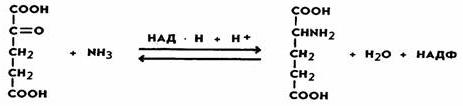
\includegraphics[width=0.7\linewidth]{pictures/glutamin}
\tetrahedral{0==COOH;3==\tetrahedral{0==C;4D==O;1==(yl);3==\tetrahedral{0==$CH_{2}$;1==(yl);3==\tetrahedral{0==$CH_{2}$;1==(yl);3==\tetrahedral{0==COOH;1==(yl)}}}}}  $+ NH_{3} \xrightarrow{\text{НАДН} + H^{+}}$ \tetrahedral{0==COOH;3==\tetrahedral{0==CHNH$_{2}$;1==(yl);3==\tetrahedral{0==$CH_{2}$;1==(yl);3==\tetrahedral{0==$CH_{2}$;1==(yl);3==\tetrahedral{0==COOH;1==(yl)}}}}} + $H_{2}O$ + НАДФ 
\end{minipage}

\caption{Схема образования глутаминовой кислоты}
\label{glutamin}
\end{figure}


%%%%%%%%%%%%%%%%%%%%%%%%%%%%%%%%%%%%%%%%%%%%%%%%%%%%%%%%%%%%%%%%%%%%%%%%%%%%%%%%%%%%%%%%%% 


\paragraph*{}Реакция присоединения аминогруппы $\alpha$-кетоглютаровой кислоте катализируется ферментом глутаматдегидрогеназой. Фермент глутаматдегидрогеназа катализирует восстановительное аминирование $\alpha$-кетоглутаровой кислоты с образованием глютаминовой кислоты. Для этой реакции необходима \gls{atp}:

%На первом этапе реакции субстраты соединяются с образованием иминокислоты, которая затем восстанавливается в глютаминовую кислоту при участии НАД(Ф)Н. Оба этапа обратимы:
 
\note{Глютаматдегидрогеназа (мол. масса 200-300 к\gls{dalton}) обнаружена в листьях и корнях у всех высших растений. Фермент локализован в митохондриях, хотя имеется в цитоплазме и в хлоропластах. Он состоит из 4-6 субъединиц. Это фермент обратимого действия и зависит от рН. Оптимум рН для аминирования на 1,5 единицы выше, чем для дезаминирования}

\paragraph*{}Образование амидов катализируется ферментом глютаминсинтетазой.
Кофакторами глютаминсинтетазы выступают ионы марганца, кобальта, кальция. Фермент обнаружен во всех органах растений и локализован в цитоплазме. 

\note{Кроме $\alpha$-кетоглутаровой кислоты, играющей основную роль в первичном связывании аммиака, в растениях аммиак может присоединятся в виде аминогруппы и к другим карбоновым кислотам, которые с помощью соответствующих ферментов взаимодействуют с $NH_{3}$, образуя так называемые первичные аминокислоты. Они же могут участвовать в различных реакциях переаминирования, когда аминогруппа переносится на них от каких либо аминокислот. К числу этих органических кислот относятся щавелевоуксусная, пировиноградная, гидроксипировиноградная, глиоксиловая и другие, в процессе восстановительного аминирования которых получаются соответственно аспарагиновая кислота, аланин, серин, глицин}

%Принято считать, что образование аспарагина преобладает в том случае, когда происходит распад белков в семенах. В клетках корня и листьев растущего растения идет, главным образом, образование глютамина. Таким образом, образование аспарагина - это путь обезвреживания аммиака, появляющегося при распаде белка - так называемая регрессивная ветвь азотного обмена, тогда как синтез глютамина - это путь обезвреживания аммиака при синтезе белка - прогрессивная ветвь азотного обмена.

\paragraph*{Роль амидов в растении}

\begin{enumerate}
	\item Растения утилизируют аммиак в форме амидов
	\item Азотные соединения транспортируются по растению в виде амидов
	\item Амиды и их предшественники аминокислоты являются материалом для создания многих других аминокислот в реакциях переаминирования, когда аминогруппа аминокислоты обменивается с кетогруппой кетокислоты с образованием аминокислоты
\end{enumerate}

\subsection*{Физиологическая роль микроэлементов}

\subsubsection*{Железо}

%Среднее содержание железа в растениях составляет 20-80 мг на 1 кг сухой массы. 
\paragraph*{Пути поступления железа в организм растения} Ионы $Fe^{3+}$ почвенного раствора восстанавливаются редокс-системами плазмалеммы клеток ризодермы до $Fe^{2+}$ и в такой форме поступают в корень. 

\paragraph*{Роль железа в растении}

\begin{enumerate}
\item Необходимо для функционирования основных редокс-систем фотосинтеза и дыхания;
\item Участвует в синтезе \hyperlink{sect_hlorophilus}{хлорофилла};
\item Для восстановления нитратов и фиксации молекулярного азота клубеньковыми бактериями, входя в состав нитратредуктазы и \hyperlink{nitrogenaza}{нитрогеназы};
\end{enumerate}

\paragraph*{}Недостаточное поступление железа в растения в условиях переувлажнения и на карбонатных почвах приводит к снижению интенсивности \hyperlink{sect_breazing}{дыхания} и \hyperlink{photosyntesis}{фотосинтеза} и выражается в пожелтении (хлорозе) листьев и быстром их опадении.

\subsubsection*{Марганец}

\paragraph*{Пути поступления марганца}

\paragraph*{}Марганец поступает в клетки в форме ионов $Mn^{2+}$ и накапливается в листьях 
%Среднее его содержание составляет 1 мг на 1 кг сухой массы. Марганец накапливается в листьях. 

\paragraph*{Роль марганца в \gls{metabolism}е растения}

\begin{enumerate}
	\item Необходим для \hyperlink{photolisys}{фотолиза воды} с выделением кислорода и восстановления углекислого газа при \hyperlink{photosyntesis}{фотосинтезе};
	\item Способствует увеличению содержания сахаров и их оттоку из листьев;
	\item активирует некоторые ферменты \note{Например, два фермента \hyperlink{krebs_cycle}{цикла Кребса} -- малат- и изоцитратдегидрогеназы - активируются ионами марганца};
	\item Необходим для функционирования нитратредуктазы при восстановлении нитратов;
	\item Является кофактором РНКполимеразы и ауксиноксидазы, разрушающей фитогормон \hyperlink{auxsin}{3-индолилуксусную кислоту};
\end{enumerate}

\paragraph*{}Cимптом марганцевого голодания -- точечный хлороз листьев, когда между жилками появляются желтые пятна, а затем клетки в этих участках отмирают. 

\subsubsection*{Молибден} 

\paragraph*{Пути поступления молибдена в растение}

%Наибольшее содержание молибдена характерно для бобовых (0,5-20 мг на 1 кг сухой массы), злаки содержат от 0,2 до 2 мг на кг сухой массы. 
\paragraph*{}Молибден поступает в растения в форме аниона $MoO_{2}^{-4}$ и концентрируется в молодых, растущих органах. В листе сосредоточен, в основном, в \hyperlink{cell_plastids}{хлоропластах}.

\paragraph*{Роль молибдена в метаболизме растения}

\begin{enumerate}
	\item Входит в состав нитратредуктазы и нитрогеназы, а также необходим для биосинтеза \hyperlink{leggemoglobin}{легоглобина};
	\item Является активатором ферментов аминирования и переаминирования, ксантиноксидаза и различных фосфатаз;
\end{enumerate}

\paragraph*{Симптомы при недостатки молибдена}

\begin{enumerate}
	\item В тканях накапливается большое количество нитратов;
	\item Не развиваются клубеньки на корнях бобовых;
	\item Наблюдаются деформации листовых пластинок. молодые листья по краям приобретают серую, а затем коричневую окраску затем ткани листа отмирают и остаются только жилки в виде хлыстиков.
\end{enumerate}

\subsubsection*{Кобальт} 

\paragraph*{Роль кобальта в метаболизме растения}
%Среднее содержание кобальта в растениях 0,02 мг на 1 кг сухой массы. 
\paragraph*{}В растениях кобальт встречается в форме иона и в  составе витамина В12.
\begin{enumerate}
\item Необходим бобовым растениям для обеспечения размножения \hyperlink{nitrificators}{клубеньковых бактерий};
\item Участвует в синтезе метионина;
\item Наряду с магнием и марганцем активирует фермент гликолиза фосфоглюкомутазу и фермент аргиназу, гидролизующий аргинин;
\end{enumerate}

\paragraph*{}Внешние признаки недостатка кобальта сходны с признаками \hyperlink{nitroHungry}{азотного голодания}.

\subsubsection*{Медь}

\paragraph*{Поступление меди в растение}

\paragraph*{}Медь поступает в клетки в форме иона $Cu^{2+}$. 
%Среднее содержание меди в растениях 0,2 мг на кг сухой массы. 

\paragraph*{}Около 70 \% всей меди, находящейся в листьях, сосредоточены в \hyperlink{cell_plastids}{хлоропластах}.

\remember{Медь входит в состав многих важных окислительно-восстановительных ферментов}

\paragraph*{Роль меди в \gls{metabolism}е}

\begin{enumerate}
\item Входит в состав \gls{plastocyanin}а -- белка-переносчика электронов между фотосистемами \gls{fs2} и \gls{fs1};
\item Входит в состав \hyperlink{enzimes}{ферментов}, катализирующих окисление аскорбиновой кислоты, дифенолов и гидроксилирование монофенолов;
\item Входит в состав ферментов дыхательной цепи \hyperlink{mitohondria}{митохондрий};
\item Входит в состав \hyperlink{nitritreductaza}{нитратредуктазного} комплекса и влияет на синтез \gls{leggemoglobin}а
\item Повышает устойчивость растений к полеганию так как влияет на активность ингибиторов роста фенольной природы;
\item Повышает засухо-, морозо- и жароустойчивость;
\end{enumerate}

\paragraph*{Недостаток меди вызывает} 

\begin{enumerate}
	\item Задержку роста и цветения;
	\item Хлороз;
	\item Потерю тургора и завядание растений;
	\item У злаков при недостатке меди не развивается колос;
	\item у плодовых появляется суховершинность;
	\item При дефиците меди белеют и отмирают кончики листьев, листья и плоды плодовых деревьев покрываются бурыми пятнами;
\end{enumerate}

\subsubsection*{Цинк}

%\paragraph*{}Содержание цинка в надземных частях бобовых и злаковых растений составляет 15-60 мг на кг сухой массы. Повышенная концентрация отмечается в листьях, репродуктивных органах и конусах нарастания, наибольшая - в семенах.

\paragraph*{Поступление цинка в растение}Цинк поступает в растение в форме катиона $Zn^{2+}$. 

\paragraph*{Роль цинка в метаболизме растения}

\begin{enumerate}
\item Необходим для функционирования ряда ферментов \hyperlink{glycolysis}{гликолиза} -- \note{Например гексокиназы, енолазы, триозофосфатдегидрогеназы, альдолазы}
\item Активирует ферменты, катализирующие расщепление угольной кислоты до углекислого газа и воды;
\note{Это помогает использованию углекислого газа в процессе \hyperlink{photosyntesis}{фотосинтеза}}
\item Участвует в образовании аминокислоты триптофана;
\note{Именно с этим связано влияние цинка на синтез белков, а также фитогормона \hyperlink{auxsin}{\gls{inodolAcid}}, предшественником которой является триптофан. Подкормка цинком способствует увеличению содержания ауксинов в тканях и активирует их рост}
\end{enumerate}

\paragraph*{Симптомы дефицита цинка}

\begin{enumerate}
\item Нарушается фосфорный обмен: \hyperlink{phosphoros}{фосфор} накапливается в корнях, задерживается его транспорт в надземные органы, замедляется превращение фосфора в органические формы.
\item Уменьшается содержание сахарозы и \hyperlink{krahmal}{крахмала};
\item Увеличивается количество органических кислот и небелковых соединений азота -- амидов и аминокислот.
\item В 2-3 раза подавляется скорость деления клеток. Это приводит к морфологическим изменениям листьев, нарушению растяжения клеток и дифференциации тканей.
\item Наиболее характерный признак цинкового голодания -- это задержка роста междоузлий и листьев, появление хлороза и развитие розеточности.
\end{enumerate}


\subsubsection*{Бор}

%\paragraph*{}Его среднее содержание составляет 0,1 мг на кг сухой массы. В боре наиболее нуждаются двудольные растения. Много бора в цветках. 
\paragraph*{}В клетках большая часть бора сосредоточена в клеточных стенках. 

\paragraph*{Роль бора в метаболизме растения}

\begin{enumerate}
\item Усиливает рост пыльцевых трубок, прорастание пыльцы, увеличивает количество цветков и плодов;
\item Снижает активность некоторых дыхательных ферментов, оказывает влияние на углеводный, белковый и нуклеиновый обмен;
\end{enumerate}

\paragraph*{Симптомы недостаток бора}

\begin{enumerate}
\item Нарушается формирование репродуктивных органов, оплодотворение, плодоношение и созревание семян;
\item Нарушаются синтез, превращения и транспорт \hyperlink{sect_glycosids}{углеводов;}
\item Так как бор не может реутилизироваться и поэтому при борном голодании прежде всего отмирают конусы нарастания, останавливается рост побегов и корней, листовые пластинки утолщаются, скручиваются, становятся ломкими, цветки не образуются. 
\end{enumerate}

\paragraph*{}Влиянию различных микроэлементов на рост растения будет посвящена одна из приведенных в данном пособии \hyperlink{mineral_elements_influence}{лабораторных работ}.

\subsection*{Вопросы и задания для самоконтроля}

\begin{enumerate}
\item Из курса экологии вы должны уже быть знакомы с таким понятием как <<\hypertarget{}{Бочка Либиха}>>. Используя учебник экологии, например за авторством Н.А. Березиной \cite{berezina_2009} и материал этого раздела, объясните, почему нехватка хотя бы одного из химических элементов является лимитирующим фактором для растения?
\item С помощью учебника ботаники повторите строение корня. Что такое \hypertarget{question_rizoderma}{ризодерма}? Как она образуется?
\item Как вы думаете, о преобладании какого типа \hypertarget{what_is_transport_type}{транспорта} веществ это свидетельствует -- активного или пассивного? Почему?
\item Какие особенности структуры молекулы какого либо вещества делают ее \hypertarget{polarMolecula}{полярной}?
\item Кукую физиологическую роль в метаболизме растений играют сера, азот, калий, кальций, магний?
\item Атомы каких элементов играют важную роль в поддержании третичной структуры белка за счет образования ковалентных связей между различными участками полипептидной цепи?
\item Какова роль леггемоглобина в процессе усвоения растениями азота?
\item Какие важные для метаболизма растения вещества синтезируются в бактероидах?
\item Вспомните, атомы каких металлов входят в состав активных центров ферментов дыхательной цепи?
\end{enumerate}


	
	%\section{Обмен и транспорт органических веществ в растениях}
	
	\section{Рост и развитие растения}
	
	%\paragraph*{}В ходе \hypertarget{ontogenesis}{онтогенеза} происходит рост и развитие организма растения.
\paragraph*{}Рост и развитие -- неотъемлемые свойства любого живого организма.

\paragraph*{}Рост растения, как и любого другого организма тесно связан с таким понятием как \gls{ontogenesis}.
\remember{Термином \gls{ontogenesis} обозначается индивидуальное развитие организма от зиготы или вегетативного зачатка до его естественной смерти.} 

\paragraph*{}В ходе \hypertarget{ontogenesis}{онтогенеза} реализуется наследственная информация организма -- генотип. А под воздействием \hyperlink{question_gen_code}{генов} и конкретных условий окружающей среды формируется фенотип -- совокупность всех признаков и свойств данного индивидуального организма.

\paragraph*{}\note{Необходимо понимать различия между понятиями \Gls{growth} и \Gls{evolution}}

\paragraph*{}\remember{\hypertarget{growth}{\Gls{growth}} -- это необратимое увеличение размеров и массы клетки, органа или всего организма растения, связанное с новообразованием элементов составляющих его структуру.

\hypertarget{evolution}{\Gls{evolution}}, же -- это качественные изменения в структуре и функциональной активности растения и его частей в процессе онтогенеза. Возникновение качественных различий между клетками, тканями и органами получило название \gls{diferintation}}

\note{Рост и развитие тесно взаимосвязаны, однако не всегда развитие сопровождается ростом. Например растение может долгое время расти и при этом находится в одной и той же фазе развития, например ювенильной. В то же время, в процессе онтогенеза растение может уменьшать свои размеры, например, когда осенью у двулетних растений отмирает надземная часть побега. Кроме того, быстрый рост может сопровождаться медленным развитием и \hyperlink{rapid_growth}{наоборот}}

\paragraph*{}Процессы роста и развития происходят на всех уровнях организации:

\begin{enumerate}
	\item Субклеточном;
	\item \hyperlink{cell_ontogenesis}{Клеточном};
	\item \hyperlink{plant_ontogenesis}{Организменном};
\end{enumerate}

\subsection*{Особенности роста клеток}

\paragraph*{}Различают следующие фазы \hypertarget{cell_ontogenesis}{\gls{ontogenesis}а} растительной клетки:

\begin{enumerate}
	\item Эмбриональная фаза;
	\item Фаза растяжения;
	\item Фаза дифференцировки;
	\item Фаза зрелости;
	\item Старение и смерть;
\end{enumerate}


\subsubsection*{Эмбриональная фаза}

\paragraph*{}Находясь на эмбриональной стадии развития клетка растения способна к делению. При этом, период существования клетки от момента её образования путём деления материнской клетки до собственного деления или гибели носит название \gls{cellCycle} (\ris \ref{cell_cykle}) Эмбриональная фаза или митотический цикл клетки делится на два периода: 

\begin{enumerate}
	\item Собственно \hyperlink{question_mitosis}{деление клетки} или  \gls{mitosis}, длительностью 2-3 часа; 
	\item Период между делениями или интерфаза длительностью 15-20 часов. В свою очередь интерфаза подразделяется на несколько периодов: 
	\begin{enumerate}
		\item Пресинтетический -- период G1 (от англ. gap – интервал). В этот перид в клетке синтезируются нуклеотиды и ферменты, необходимые для синтеза \gls{dna}. Происходит синтез \gls{rna}.
		\item Синтетический периож -- S. В данный период происходит удвоение \gls{dna} и образование белков-гистонов.
		\item Премитотический период -- G2. В течении данного периода продолжается синтез \gls{rna} и белков. Репликация митохондриальной и пластидной \gls{dna} происходит на протяжении всей интерфазы.
	\end{enumerate}
\end{enumerate}

%%%%%%%%%%%%%%%%%%%%%%%%%%%%%%%%%%%%%%%%%%%%%%%%%%%%%%%%%%%%%%%%%%%%%%%%%%%%%%%%%%%%%%%%%%%%%%%%%%%%%%%%%%% 
\begin{figure}
  \centering
       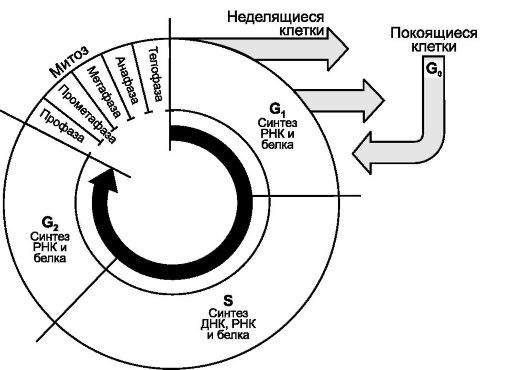
\includegraphics[width=0.5\linewidth]{pictures/cell_cykle}
\caption{Схема клеточного цикла}

\label{cell_cykle}
\end{figure}
%%%%%%%%%%%%%%%%%%%%%%%%%%%%%%%%%%%%%%%%%%%%%%%%%%%%%%%%%%%%%%%%%%%%%%%%%%%%%%%%%%%%%%%%%% 

\paragraph*{}\note{Клетки образовательных тканей находятся на эмбриональной стадии в течении всей своей жизни}

\subsubsection*{Фаза растяжения}

\paragraph*{}Прекратившие деление клетки переходят к росту путем \hypertarget{strainGrowth}{растяжения}. Процесс роста клетки растяжением можно описать следующей цепочкой событий:

\begin{enumerate}
	\item Под действием гормона \hyperlink{auxin}{ауксина} активируется транспорт протонов в \hyperlink{cell_wall}{клеточную стенку}
	\item \hyperlink{cell_wall}{Клеточная стенка} разрыхляется, становится более упругой, вследствие чего в \hyperlink{cell_vakuol}{центральную вакуоль} клетки начинает поступать вода.
	\item Растущая клетка начинает увеличиваться в размерах за счет образования большой \hyperlink{cell_vakuol}{центральной вакуоли} и формирования органелл и цитоплазмы. 
	\item В везикулах аппарата Гольджи из галактуроновой кислоты начинает синтезироваться пектин, а на наружной стороне плазмалеммы -- \hyperlink{cellulosa}{целлюлозные волокна}
	\item В \hyperlink{cell_wall}{клеточную стенку} начинают включатся новые волокна целлюлозы и пектиновые вещества. 
	\item В конце фазы растяжения усиливается лигнификация клеточных стенок, что снижает ее упругость и проницаемость, накапливаются ингибиторы роста, повышается активность оксидазы \gls{inodolAcid}, снижающей содержание \hyperlink{auxsin}{ауксина} в клетке.
\end{enumerate}

\subsubsection*{Фаза дифференцировки}

\paragraph*{}На данной стадии клетка приобретает морфологические и физиологические особенности, необходимые ей для дальнейшего функционирования в составе определенной ткани (\ris \ref{plants_cells}) В основе процессов дифференцировки лежит изменение активности или \gls{genExpression} различных генов. 

%%%%%%%%%%%%%%%%%%%%%%%%%%%%%%%%%%%%%%%%%%%%%%%%%%%%%%%%%%%%%%%%%%%%%%%%%%%%%%%%%%%%%%%%%%%%%%%%%%%%%%%%%%% 
\begin{figure}[h!]
  \centering
       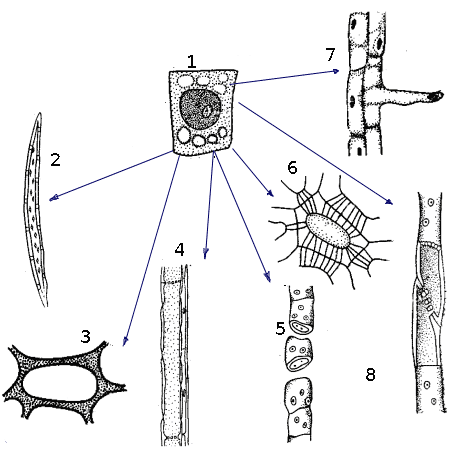
\includegraphics[width=0.5\linewidth]{pictures/plants_cells}
\caption{Различные типы растительных клеток}
\label{plants_cells}
\end{figure}
%%%%%%%%%%%%%%%%%%%%%%%%%%%%%%%%%%%%%%%%%%%%%%%%%%%%%%%%%%%%%%%%%%%%%%%%%%%%%%%%%%%%%%%%%% 

\paragraph*{}\remember{Сигналами для экспрессии только определенных генов служат сочетания фитогормонов, метаболитов и физико-химических факторов (например, давление соседних клеток)}

\paragraph*{}Таким образом, каждая клетка растения содержит в своем геноме полную информацию о развитии всего организма и, потенциально, может дать начало формированию целого растения. Данное свойство носит название \gls{totipatentia}. 

\paragraph*{}Однако, находясь в составе организма, эта клетка будет реализовать только часть своей генетической информации. 

\subsubsection*{Фаза зрелости} 

\paragraph*{}Зрелая клетка начинает выполнять функции, свойственные клеткам той \hyperlink{plants_tisues}{ткани}, в состав которой она входит.

\paragraph*{}\note{Некоторые ткани состоят из мертвых клеток. Такими тканями являются, например ксилема и склеренхима}

\subsubsection*{Старение и смерть}

\paragraph*{}Старение и смерть клетки происходит в результате:

\begin{enumerate}
\item Накопления повреждений в генетическом аппарате, клеточных мембранах и включениях;
\item Генетической програмированной клеточной; смерти\footnote{генетически запрграммированная смерть клеток животных называется апоптоз}
\end{enumerate}

\paragraph*{}При старении клеток происходит усиление процессов гидролиза входящих в состав клетки веществ и одновременное ослабление процессов синтеза новых веществ. В органеллах и цитоплазме образуются автофагические вакуоли, разрушаются \hyperlink{sect_hlorophilus}{хлорофилл} и \hyperlink{cell_plastids}{хлоропласты}, эндоплазматический ретикулум, аппарат Гольджи, ядрышко, набухают \hyperlink{mitohondria}{митохондрии}, в них снижается число крист, вакуолизируется ядро. 

\remember{Гибель клетки становится необратимой после разрушения \hyperlink{plasmolema}{клеточных мембран}, в том числе и \hyperlink{cell_vakuol}{тонопласта}, выхода содержимого вакуоли и лизосом в цитоплазму}

\subsection*{Этапы онтогенеза высших растений} 

\paragraph*{}Каждый растительный организм в своем \hypertarget{plant_ontogenesis}{развитии} проходит ряд этапов, характеризующихся морфологическими и физиологическими особенностями.

%%%%%%%%%%%%%%%%%%%%%%%%%%%%%%%%%%%%%%%%%%%%%%%%%%%%%%%%%%%%%%%%%%%%%%%%%%%%%%%%%%%%%%%%%%%%%%%%%%%%%%%%%%% 
\begin{figure}[h!]
  \centering
       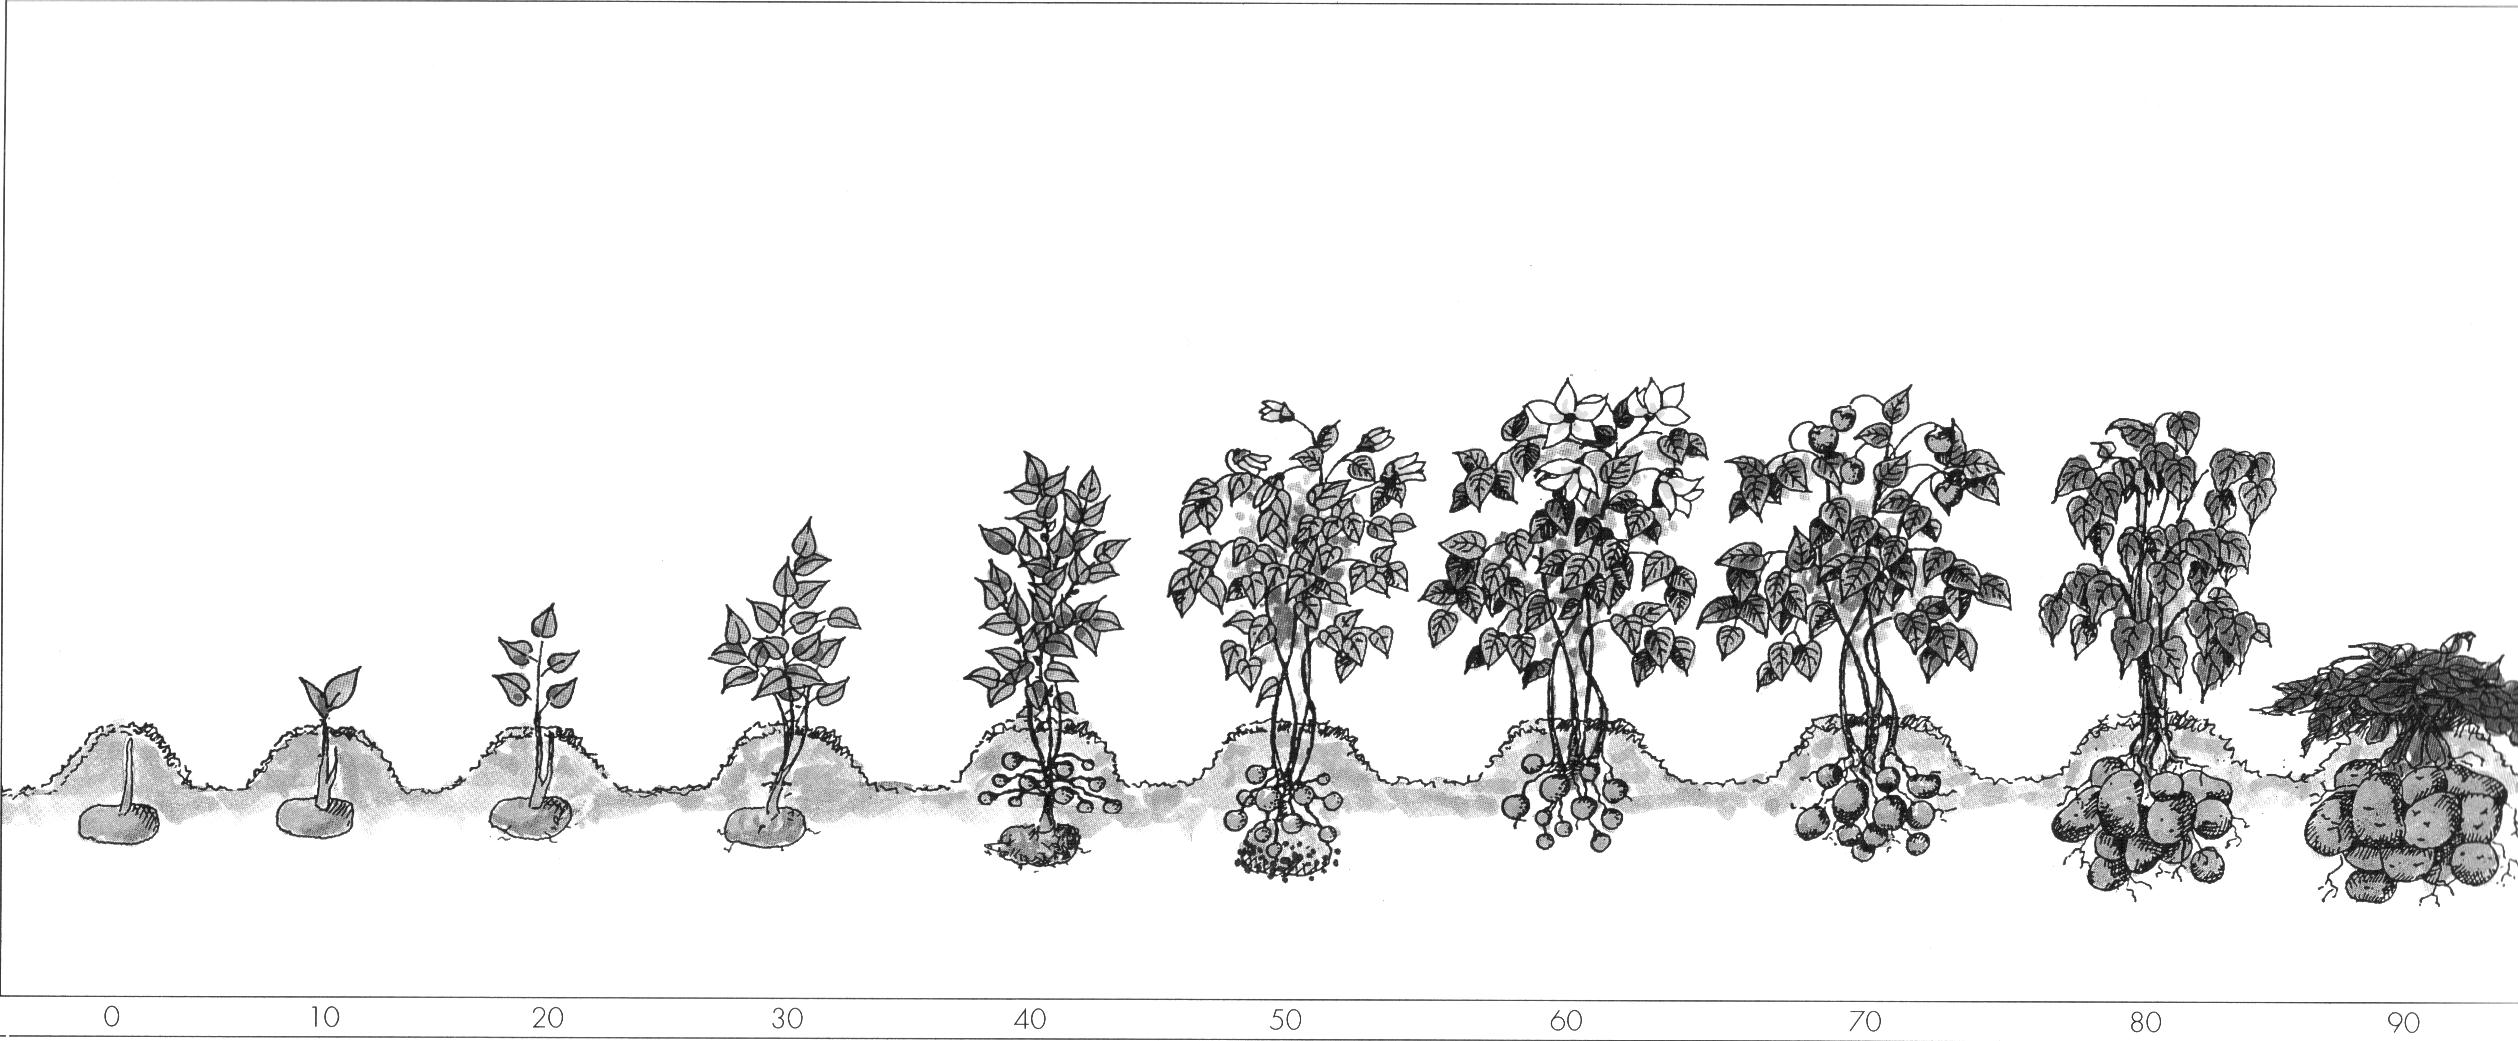
\includegraphics[width=0.7\linewidth]{pictures/ontogenesis_stages}
\caption{Этапы онтогенеза растения}
\label{ontogenesis_stages}
\end{figure}
%%%%%%%%%%%%%%%%%%%%%%%%%%%%%%%%%%%%%%%%%%%%%%%%%%%%%%%%%%%%%%%%%%%%%%%%%%%%%%%%%%%%%%%%%% 

\subsubsection*{Ювенильный этап} 

\paragraph*{}Ювенильный этап (\ris \ref{ontogenesis_stages}) начинает с прорастания семян или органов вегетативного размножения и характеризуется накоплением вегетативной массы. Растения на этом этапе не способны к половому размножению.

\subsubsection*{Этап зрелости и размножения}

\paragraph*{}Зрелое (взрослое) растение способно к половому размножению. Происходит формирование генеративных органов и образование плодов. 
\paragraph*{}У растений выделяют следующие типы размножения:

\begin{enumerate}
	\item \gls{sexualMaturing}, когда новый организм появляется в результате слияния половых клеток -- гамет;
	\item \gls{asexualMaturing}, когда новый организм развивается из спор;
	\item \gls{vegetationMaturing} -- воспроизведение растений из вегетативных частей растения (клубней, луковиц, отводок)
\end{enumerate};

%\paragraph*{}\note{Бесполое размножение характерно для споровых растений}

\paragraph*{}\gls{life_cycle} всех растений характеризуется чередованием двух поколений -- гаплоидного \gls{gametophit}а и диплоидного \gls{sporophit}а. При этом, эволюция растений была направлена в сторону постепенной редукции гаметофита. Так, у споровых растений гаметофит и спорофит являются самостоятельными организмами. У семянных же растений гаметофит утратил самостоятельность, женский гаметофит существует в виде семязачатка внутри завязи цветка, а мужской гаметофит -- это пыльцевое зерно (\ris \ref{life_cycle} б).

%%%%%%%%%%%%%%%%%%%%%%%%%%%%%%%%%%%%%%%%%%%%%%%%%%%%%%%%%%%%%%%%%%%%%%%%%%%%%%%%%%%%%%%%%%%%%%%%%%%%%%%

\begin{figure}[h]
\begin{minipage}[h]{0.49\linewidth}
\center{\includegraphics[width=0.9\linewidth]{pictures/i_103} \\ а) Папоротники}
\end{minipage}
\hfill
\begin{minipage}[h]{0.49\linewidth}
\center{\includegraphics[width=0.9\linewidth]{pictures/i_125} \\ б) Цветковые растения}
\end{minipage}
\caption{Схема жизненного цикла споровых и цветковых растений}
\label{life_cycle}
\paragraph*{}Схема взята из \cite{sonin_bio}
\end{figure}

%%%%%%%%%%%%%%%%%%%%%%%%%%%%%%%%%%%%%%%%%%%%%%%%%%%%%%%%%%%%%%%%%%%%%%%%%%%%%%

\paragraph*{}В зависимости от количества циклов полового размножения в жизненном цикле, все растения делятся на две большие группы: 

\begin{enumerate}
	\item \gls{monokarpics} (плодоносящие один раз). К монокарпическим относятся все однолетние растения, некоторые двулетние и многолетние.
	\item \gls{polykarpics} (плодоносящие многократно). Большинство многолетних растений
\end{enumerate}

\paragraph*{}Среди монокарпических растений выделяют такие жизненные формы, как

\begin{enumerate}
	\item \gls{ephemers} -- растения, \gls{life_cycle} которых занимает всего несколько недель
	\item Однолетники (яровые и озимые злаки, картофель, бобовые)
	\item Двулетники (корнеплоды, капуста, лук)
	\item Многолетники (агавы, некоторые пальмы)
\end{enumerate} 

\paragraph*{}В свою очередь, серди поликарпических растений выделяют виды, цветущие на \cite{rubin_71}:

\begin{enumerate}
	\item 1-ый год жизни (ряд многолетних злаков);
	\item 2-ой год жизни (люцерна, многолетний люпин);
	\item 3-ий год жизни (ягодные кустарники);
	\item 8-12 год жизни (яблоня, груша);
	\item 25-30 год жизни (липа, клен);
	\item 40-60 год жизни (дуб);
\end{enumerate}

\paragraph*{}Инициация перехода к цветению осуществляется под действием внешних факторов, таких как температура (\gls{jarovisation}), чередование дня и ночи (\gls{photoperiodism}) или эндогенных факторов, обусловленных возрастом растения. Растения, нуждающиеся в яровизации, называют озимыми, а развивающиеся без нее -- яровыми. 

%Яровизация – это неизвестный пока процесс, протекающий в растениях под действием низких положительных температур и способствующий последующему ускорению развития растений. 
\note{Различия между озимыми и яровыми формами зерновых культур обусловлены генетически. Так, озимая и яровая рожь различаются всего по одному гену}

\paragraph*{}В зависимости от реакции на длину дня, растения делятся на

\begin{enumerate}
	\item Короткодневные, переходящие к цветению только тогда, когда день короче ночи (рис, соя);
	\item Длиннодневные (хлебные злаки, крестоцветные, укроп); 
	\item Растения, нуждающиеся в чередовании разных фотопериодов, а также 
	\item Нейтральные по отношению к длине дня (гречиха, горох);
\end{enumerate}

\note{Длиннодневные растения распространены, в основном, в умеренных и приполярных широтах, короткодневные -- в субтропиках}

\paragraph*{}У большинства растений наибольшей чувствительностью к фотопериоду обладают листья, только что закончившие рост. Основную роль в восприятии фотопериода играет белок \hyperlink{phitochrom}{фитохром}, который под действием света может менять свою конформацию.

%Показано участие в переходе к цветению стимулятора роста гиббереллина. В условиях неблагоприятного фотопериода в листья обнаруживаются ингибиторы цветения. 
\paragraph*{}Цветы -- это органы полового размножения (\gls{generativeOrgans}). Цветки как органы полового размножения могут быть обоеполыми или раздельнополыми. Они формируются на одних и тех же (однодомность) или на разных (двудомность) растениях. 

\paragraph*{}Факторы внешней среды, приводящие к увеличению содержания в растении цитокининов и \hyperlink{auxsin}{ауксинов}, увеличивают долю женских цветков, а повышающие концентрацию гиббереллинов -- мужских.

\paragraph*{Двойное оплодотворение}

\paragraph*{}Одной из особенностей цветковых растений является двойное оплодотворение. При этом, в процессе оплодотворения выделяют три фазы:

\begin{enumerate}
	\item Опыление, когда пыльцевое зерно попадает на рыльце пестика;
	\item Прорастание пыльцы и рост пыльцевой трубки в тканях пестика;
	\item Собственно оплодотворение, то есть образование зиготы;
\end{enumerate}

\paragraph*{}При двойном оплодотворении зигота образуется при слиянии спермия пыльцевой трубки (мужской \gls{gametophit}) с яйцеклеткой зародышевого мешка (женский \gls{gametophit}). В это же время, второй спермий соединяется с вторичным диплоидным ядром центральной клетки зародышевого мешка. 
%Зародыши проходят ряд последовательных фаз развития. На последнем этапе созревания семена теряют значительное количество воды и переходят в состояние покоя, когда в тканях уменьшается содержание стимуляторов роста и увеличивается количество ингибитора роста абсцизовой кислоты.

\paragraph*{}Плод развивается из завязи цветка и, как правило, содержит семена. Плоды могут формироваться без оплодотворения и образования семян. Это явление называется \gls{partenokarpia}. Образование партенокарпических (бессемянных) плодов может происходить при обработке растений \hyperlink{auxsin}{ауксинами} и гиббереллинами. Однако обычно цветки без опыления и оплодотворения опадают.

\subsubsection*{Этап старости и отмирания}

\paragraph*{}Этап старости и отмирания (\ris \ref{ontogenesis_stages}) включает в себя период от полного прекращения плодоношения до смерти организма. Для него характерно прогрессирующее ослабление жизнедеятельности. 

\paragraph*{}У многих растений периодически отмирают отдельные элементы побега:
\begin{enumerate}
	\item Однолетние растения погибают целиком;
	\item У многолетних трав ежегодно полностью отмирает надземная часть, а корневая система остается жизнеспособной;
	\item У многих растений стареют и опадают ранее образовавшиеся листья;
	\item У листопадных деревьев осенью одновременно стареют и опадают все листья одновременно. 
\end{enumerate}

\paragraph*{}Перед опадением листа или плода в основании черешка листа или плодоножки образуется отделительный слой -- зона, где у клеток размягчаются и частично растворяются клеточные стенки и срединные пластинки. Этот процесс начинается под воздействием этилена, который вырабатывается стареющими листьями и созревающими плодами.

\subsection*{Дифференцировка и рост растений}

\paragraph*{}У животных в течение жизни происходит лишь увеличение размеров заложенного перед рождением органа, а у растений -- заложение и увеличение размеров органа идет параллельно в течение всего онтогенеза

\remember{Характерной  чертой растений является то, что новые ткани и органы растений формируются за счет деятельности специальной образовательной ткани, которая носит название \gls{meristema}}

\paragraph*{}Существование меристем поддерживается инициальными клетками \gls{initialCells}, длительное время способными к делению путем митоза. 

\note{У мхов, хвощей и папоротников в апикальной меристеме имеется только одна инициалия в виде трехгранной пирамиды с выпуклым основанием, у других высших растений инициалий несколько и они трудноотличимы от остальных клеток \gls{apex}а \cite{korowkin_gloss}}.

\paragraph*{}Более длительная способность к делению является следствием меньшей частоты делений и большей длительности интерфазы.

\paragraph*{}Различают следующие типы меристем:

\begin{enumerate}
	\item Апикальные (верхушечные) \gls{meristema} расположены на концах побегов и корней --\gls{apex}ах (\ris \ref{apex}). Апикальные меристемы побега и корня представляют собой не только образовательные ткани, но и главные координирующие центры влияющие на морфогенетические процессы в целом растении;
	\note{Так как кончики растущего корня или стебля первыми ощущают на себе действие факторов окружающей среды, в них расположены многие рецепторные системы растения}
	\item Латеральные (боковые) \gls{meristema} образуют слои клеток вдоль побега и корня В результате деления клеток камбия образуются ксилема и флоэма;
	\item Интерколлярные или вставочные \gls{meristema} -- расположены в основании междоузлий и листьев;
\end{enumerate}

%%%%%%%%%%%%%%%%%%%%%%%%%%%%%%%%%%%%%%%%%%%%%%%%%%%%%%%%%%%%%%%%%%%%%%%%%%%%%%%%%%%%%%%%%%%%%%%%%%%%%%%%%%% 
\begin{figure}[h!]
  \centering
       \includegraphics[width=0.3\linewidth]{pictures/apex}
\caption{Апекс побега эллодеи}
\paragraph*{}Рисунок приведен согласно \cite{korovkin_2007}
\label{apex}
\end{figure}
%%%%%%%%%%%%%%%%%%%%%%%%%%%%%%%%%%%%%%%%%%%%%%%%%%%%%%%%%%%%%%%%%%%%%%%%%%%%%%%%%%%%%%%%%% 


\paragraph*{}\gls{morphogenesis}, то есть формообразование у растений включает в себя процессы заложения, роста и развития

\begin{enumerate}
	\item Клеток (цитогенез);
	\item Тканей (гистогенез);
	\item Оганов (органогенез);
\end{enumerate}
\remember{Процессы морфогенеза генетически запрограммированы и скоординированы между собой} 

%Межклеточные системы регуляции включают гормональные, электрические и трофические факторы, которые влияют на генетическую, мембранную и метаболическую регуляторные системы в каждой клетке. 

\paragraph*{}Включение и выключение генетических программ в клетке зависит от поступления в клетку сигналов, особенно \hyperlink{gormons}{фитогормонов}, из других клеток. 

%Ауксин необходим для включения генетической программы корнеобразования, а цитокинин в присутствии ауксина вызывает экспрессию генов, ответственных за программу побегообразования.
\paragraph*{}В процессе морфогенез растительного организма наблюдается поляризация развития отдельных структур. \gls{polarisation} биологических структур -- это ориентация процессов и структур в пространстве, то есть физиолого-биохимические и анатомо-морфологические свойства изменяются в определенном направлении. 

\paragraph*{}\gls{polarisation} вызывается:

\begin{enumerate}
	\item Градиентами осмотического давления;
	\item pH;
	\item Концентрации кислорода и углекислого газа;
	\item Гормональными, электрическими и трофическими контактами с соседними клетками;
	\item Механическим давлением;
\end{enumerate}

%\paragraph*{}В результате в клетках реализуются именно те потенции, которые соответствуют окружающим условиям. 

\note{У растительных клеток найдены рецепторы фитогормонов, позволяющие клеткам <<ощущать>> наличие гормонов в окружающей среде. При культивировании клеток в искусственной среде проявляется так называемый <<эффект массы>>. Он выражается в том, что единичная изолированная клетка редко переходит к делению. Чем гуще суспензия клеток, тем большее их число начинает делиться. Для дифференциации большое значение имеет наличие в клеточной стенке белков лектинов, участвующих в узнавании и взаимодействии клеток}

\paragraph*{}В процессе роста наблюдается также зависимость роста и развития одних органов от других -- \gls{growthCorrelations}. 

\note{Например, очевидно, что развитие побега зависит от корня, поставляющего минеральные вещества и воду. В свою очередь, побег поставляет в корень органические соединения. По этой причине, площадь коневой системы дерева сопоставима с площадью его кроны} 

\paragraph*{}Основную роль в процессе роста играют гормональные взаимодействия между частями растения. 

\note{Примером гормональной регуляции служит явление апикального доминирования, которое заключается в торможении верхушкой побега или корня развития соответственно пазушных почек или боковых корней}

\paragraph*{}\gls{apexDominance} доминирование обусловлено тем, что:

\begin{enumerate}
	\item Точка роста побега, содержащая большое количество \hyperlink{auxsin}{ауксина}, является мощным центром, притягивающим питательные вещества и гормон \hyperlink{citokin}{цитокин} синтезированный в корне;
	\item \hyperlink{auxsin}{Ауксин} задерживает образование проводящих пучков, соединяющих боковые почки с центральной проводящей системой;
\end{enumerate}

\paragraph*{}\gls{apexDominance} исчезает при удалении апекса центрального побега. После этого начинается интенсивный рост боковых побегов.

%Удаление верхушки побега стимулирует этот процесс, а приток цитокинина к пазушным почкам усиливает в них клеточные деления. Формирующиеся в боковых почках листовые зачатки начинают синтезировать ауксин, необходимый для дальнейшего развития боковых побегов.

\note{Ростовые корреляции используются в растениеводстве для получения большего количества продукции. Например, пасынкование -- удаление боковых побегов у томатов способствует образованию более крупных плодов, пикировка -- обрывание кончиков корней при пересадке рассады овощей увеличивает число боковых корней}

\paragraph*{}Процессам роста, как и другим физиологическим явлениям, свойственна периодичность, которая вызывается как особенностями самих процессов, так и факторами внешней среды. 

\paragraph*{}Наиболее распространены в организме растения процессы с периодичностью около суток. К таким процессам относятся 

\begin{enumerate}
\item Изменения митотической активности в меристемах
\item \hyperlink{photosyntesis}{Фотосинтез}
\item \hyperlink{sect_breazing}{Дыхание}
\item Открытие и закрытие цветков
\end{enumerate}

\paragraph*{}Суточные ритмы связаны с суточными колебаниями освещенности и температуры. 

\paragraph*{}Кроме суточной для растений характерна сезонная периодичность, заключающаяся в наступлении периодов покоя. Различают следующие типы покоя:

\begin{enumerate}
\item \gls{necessityRepose}, обусловленный факторами внешней среды, препятствующими прорастанию;
\item Физиологический покой (глубокий покой), который регулируется балансом стимуляторов и ингибиторов роста
\end{enumerate}

%При вступлении в период покоя происходят процессы, повышающие устойчивость клеток к неблагоприятным факторам среды: возрастает вязкость цитоплазмы, она отходит от клеточных стенок, что нарушает связь между клетками, снижается интенсивность процессов обмена. Сухие семена не прорастают до тех пор, пока не будет достаточного количества воды. Весной почки не распускаются, пока не поднимется до определенного уровня температура. 

\paragraph*{}Из состояния вынужденного покоя растение выходит как только условия окружающей среды становятся благоприятными.

\paragraph*{}Растения, находящиеся в физиологическом покое, не переходят к росту даже при благоприятных условиях среды. Для выхода семян из глубокого покоя их подвергают стратификации. \gls{stratification} заключается в выдерживании влажных семян при пониженной температуре.

%\subsection*{Регенерация у растений} 

%Регенерация – это восстановление организмом поврежденной или утраченной части тела, что является одним из способов вегетативного размножения и защиты растений от повреждений. Различают следующие виды регенерации.
%I. Физиологическая регенерация.
%Части восстанавливаются при их естественном изнашивании, например, постоянное восполнение слущивающихся клеток корневого чехлика.
%II. Травматическая регенерация.
%1. Регенерация, обусловленная дедифференцировкой клеток:
%а) заживление ран.
%Эпидермис и первичная кора дедифференцируются, их клетки начинают делиться и образуют вторичную меристему, которая превращается в пробку.
%б) органогенез, связанный с образованием каллуса.
%Клетки дедифференцируются и переходят к неорганизованному делению, образуя каллусную ткань из рыхло соединенных друг с другом паренхимных клеток. Иногда отдельные клетки дают начало адвентивным, то есть возникшим не из эмбриональных тканей, органам: корням, побегам, листьям.
%в) соматический эмбриогенез.
%На раневой поверхности образуется каллус. Из отдельных клеток каллуса, начинающих делиться, формируются соматические зародыши (эмбриоиды), из которых при определенных условиях развивается целый организм.
%г) восстановление частей без образования каллуса.
%Паренхимные клетки коры под влиянием ауксина, индуцирующего генетическую программу ксилемообразования, превращаются в клетки ксилемы при образовании обходного участка проводящего пучка вокруг места его прерывания.
%2). Регенерация на уровне меристем:
%а) восстановление апикальных меристем.
%При продольном рассечении конуса нарастания из каждой половины могут регенерировать отдельные апексы.
%б) органогенез из предсуществующих зачатков.
%Восстановление надземных органов у высших растений происходит за счет отрастания пазушных почек при устранении доминирующего влияния апекса побега.

\subsection*{Кинетика ростовых процессов} 

\paragraph*{}Кривую, описывающую скорость роста, можно разделить на 4 участка (\ris \ref{growth_line}): 

\begin{enumerate}
	\item Лаг-период -- рост почти не заметен и идут процессы, подготавливающие организм к видимому росту;
	\item Лог-фаза -- скорость роста изменяется логарифмически;
	\item Фаза замедления роста;
	\item Стационарная фаза;
\end{enumerate}

%%%%%%%%%%%%%%%%%%%%%%%%%%%%%%%%%%%%%%%%%%%%%%%%%%%%%%%%%%%%%%%%%%%%%%%%%%%%%%%%%%%%%%%%%%%%%%%%%%%%%%%%%%% 
\begin{figure}[h!]
  \centering
       \includegraphics[width=0.5\linewidth]{pictures/growth_line}
\caption{Кривая роста}
\label{growth_line}
\end{figure}
%%%%%%%%%%%%%%%%%%%%%%%%%%%%%%%%%%%%%%%%%%%%%%%%%%%%%%%%%%%%%%%%%%%%%%%%%%%%%%%%%%%%%%%%%% 

%1 – лаг-период, 2 – логарифмическая фаза, 3 – фаза замедленного роста, 4 – фаза стационарного состояния (по С. И. Лебедеву).

\paragraph*{}Для измерения скорости роста используются следующие показатели.

\paragraph*{}\gls{growthRate} r -- прирост массы растения или отдельного его органа в единицу времени, который рассчитывается по формуле Блекмана \ref{blekman} \cite{malinowsky_2004}

\begin{equation}
	r=\frac{\lg{\frac{W_{1}}{W_{0}}}} x 2,3026
		{t}
		\label{blekman}
\end{equation}
   
\paragraph*{}где $W_{0}$ – начальный, а $W_{1}$ – конечный вес сухого вещества, t – промежуток времени между определениями.

\paragraph*{}\gls{relativeGrowthRate} R -- прирост, вычисленный в процентах от исходного веса растения или органа \ref{relative_growth}:            

\begin{equation}
	R=\frac{W_{1}-W_{0}}{W_{0}} x 100
	\label{relative_growth}
\end{equation}

\paragraph*{}\gls{absoluteGrowthRate} К -- величина прироста за промежуток времени, отнесенная к единице времени \ref{absolute_growth}:

\begin{equation}
	K=\frac{W_{2}-W_{1}}{t_{2}-t_{1}}
	\label{absolute_growth}
\end{equation}


\subsection*{Влияние факторов внешней среды на рост растений}

На рост растений оказывают влияние такие факторы, как

\begin{enumerate}
	\item Продукты жизнедеятельности одних растений могут подавлять рост других -- аллелопатия;
	\item Продукты жизнедеятельности микроорганизмов (антибиотики, регуляторы роста) 
	\item Факторы внешней среды, такие как температура воздуха, уровень освещенности и т.д.
\end{enumerate} 

\subsubsection*{Свет}

\paragraph*{}Растения воспринимают свет не только как источник энергии, но и в качестве сигнала, характеризующего условия среды. Растение воспринимают изменение длинны светового дня с помощью специальных молеку-рецепторов -- \hypertarget{phitochrom}{фитохрома}, опосредующего действие света на морфогенез. \gls{phitochrom} состоит из двух белковых субъединиц и хромофора – незамкнутого тетрапиррола, относящегося к группе фикобилинов. \gls{phitochrom} синтезируется в форме, поглощающей красный свет (Ф660). Под действием красного света эта форма фитохрома переходит в активную форму, поглощающей дальний красный свет (Ф730). Под действием дальнего красного света и в темноте Ф730 превращается обратно в Ф660. 
\paragraph*{}Фитохром оказывает на клетку следующие физиологическое воздействие: 

\begin{enumerate}
	\item Изменяет проницаемость \hyperlink{plasmolema}{клеточных мембран};
	\item Регулирует движение \hyperlink{cell_plastids}{хлоропластов};
	\item Влияет на синтез ферментов и стимуляторов роста \hyperlink{gybberelin}{гиббереллинов} и \hyperlink{citokin}{цитокининов};
\end{enumerate}

\subsubsection*{Температура}

\paragraph*{}Различают три основные температурные точки: 

\begin{enumerate}
	\item Минимальная температура, при которой начинается рост растения;
	\item Оптимальная температура, наиболее благоприятная для роста растения;
	\item Максимальная, при которой рост растения прекращается;
\end{enumerate}

\paragraph*{}В зависимости от приспособленности к температурному режиму различают:

\begin{enumerate}
	\item Теплолюбивые растения (минимальная температура выше 10~ \celsius, оптимальная 30-40~ \celsius)
	\item Холодостойкие растения (минимальная температура 0-5~ \celsius, оптимальная 25-30~ \celsius)
\end{enumerate}


%\subsubsection*{Газовый состав атмосферы}
%Газовый состав. Необходим кислород, так как дыхание поставляет энергию для ростовых процессов, и углекислый газ, который в ходе фотосинтеза восстанавливается до органических веществ. Избыток углекислого газа на короткое время повышает растяжимость клеточных стенок и стимулирует рост клеток (эффект «кислого роста»).

\subsubsection*{Водный режим}
\paragraph*{}Недостаточное снабжение растений водой задерживает рост побегов и кратковременно стимулирует с последующим торможением рост корней. 

\subsubsection*{Минеральное питание}
\paragraph*{}Для нормального роста необходимо достаточное снабжение всеми питательными элементами. 
%Избыток азота стимулирует рост вегетативной массы, но замедляет процессы дифференцировки и формирование цветков.

\subsection*{Фитогормоны} 

\paragraph*{}\hypertarget{gormons}{\gls{phitogormons}} образуются в процессе обмена веществ растений и оказывают в очень малых количествах регуляторное и координирующее влияние на физиологические процессы в разных органах. Различают стимуляторы и ингибиторы роста. 

\remember{Следует помнить, что стимуляторы роста, применяемые в сверхоптимальных дозах, способны подавлять ростовые процессы}

\subsubsection*{Ауксины}

\paragraph*{}Главным представителем \hypertarget{auxsin}{\gls{auxin}ов} в растениях является \gls{inodolAcid} (\ris \ref{growth_stimulators}) Она синтезируется из триптофана в верхушке побега. Разрушается \gls{inodolAcid} ферментом ИУК-оксидазой. 

\paragraph*{}Ауксин оказывает стимулирующие влияние на следующие процессы, происходящие в растении:

\begin{enumerate}
	\item Стимулирует деление и растяжение клеток;
	\item \gls{inodolAcid} активирует протонную помпу в плазмалемме, что приводит к закислению и разрыхлению \hyperlink{cell_wall}{клеточной стенки} во время роста клетки за счет \hyperlink{strainGrowth}{растяжения};
	\item Необходим для образования проводящих пучков и корней;
	\item Комплекс \gls{inodolAcid} с рецептором транспортируется в ядро и активирует синтез \gls{rna}, что в свою очередь, приводит к усилению \hyperlink{proteinSintez}{синтеза} \hyperlink{proteins}{белков};
\end{enumerate}

%%%%%%%%%%%%%%%%%%%%%%%%%%%%%%%%%%%%%%%%%%%%%%%%%%%%%%%%%%%%%%%%%%%%%%%%%%%%%%%%%%%%%%%%%%%%%%%%%%%%%%%

\begin{figure}[h]
\begin{minipage}[h]{0.49\linewidth}
\center{\includegraphics[width=0.7\linewidth]{pictures/auxin} \\ а) Ауксин}
\end{minipage}
\hfill
\begin{minipage}[h]{0.49\linewidth}
\center{\includegraphics[width=0.9\linewidth]{pictures/gibberelin} \\ б) Гибберелин}
\end{minipage}
%\caption{Зависимость сигнала от шума для данных.}
\label{growth_stimulators}
\end{figure}

%%%%%%%%%%%%%%%%%%%%%%%%%%%%%%%%%%%%%%%%%%%%%%%%%%%%%%%%%%%%%%%%%%%%%%%%%%%%%%

\subsubsection*{Цитокинины}
\paragraph*{}\hypertarget{citokin}{Цитокинины} образуются путем конденсации аденозин-5-монофосфата и изопентенилпирофосфата в апикальной меристеме корня. Много цитокининов в развивающихся семенах и плодах. 
\paragraph*{}Цитокины стимулируют следующие процессы:

\begin{enumerate}
	\item В присутствии вызывает \hyperlink{auxsin}{ауксина} деление клеток;
	\item Активируют дифференциацию \hyperlink{cell_plastids}{пластид};
	\item Повышают активность АТФ-синтетазы;
	\item Способствуют выходу почек, семян и клубней из состояния покоя;
	\item Предотвращают распад \hyperlink{sect_hlorophilus}{хлорофилла} и деградацию клеточных органелл;
	\item Комплекс цитокининов с белковым рецептором повышает активность \gls{rna}-полимеразы. При повышается \gls{genExpression} этом увеличивается число полисом и активируется синтез белка;
\end{enumerate}

\subsubsection*{Гиббереллины}

\note{В настоящее время известно более 70 \hypertarget{gybberelin}{гиббереллинов} кислой и нейтральной природы} 

\paragraph*{}Наиболее известным и распространенным гиббереллином является гибберелловая кислота (\ris \ref{growth_stimulators}). Исходным веществом для синтеза гибберелинов является \gls{acetylCoensimA}. \gls{gibberelins} синтезируются  в листьях и корнях. 

\paragraph*{}\gls{gibberelins} способствуют:

\begin{enumerate}
	\item Удлинению стебля;
	\item Выходу семян из состояния покоя;
	\item Формированию гранулярного эндоплазматического ретикулума;
	\item Образованию цветоноса и цветению;
	\item Активируют деление клеток в апикальных и интеркалярных меристемах;
	\item Повышают активность \hyperlink{enzimes}{ферментов} синтеза \hyperlink{plipids}{фосфолипидов};
	\item Комплекс гиббереллина с белковым цитоплазматическим рецептором стимулирует синтез нуклеиновых кислот и \hyperlink{proteins}{белка};
\end{enumerate}

\subsubsection*{Абсцизовая кислота}

\paragraph*{}Cинтезируется в листьях и корневом чехлике двумя путями: из мевалоновой кислоты или путем распада каротиноидов. \hypertarget{abscizeAcid}{\gls{abscizeAcid}} тормозит рост растений и является антагонистом стимуляторов роста. 

\paragraph*{}\note{Однако у огурца \gls{abscizeAcid} активирует удлинение гипокотиля, а у черенков фасоли образование корней} 

\paragraph*{}\gls{abscizeAcid} ускоряет распад нуклеиновых кислот, белков, \hyperlink{sect_hlorophilus}{хлорофилла}, ингибирует мембранную протонную помпу. 

\paragraph*{}\gls{abscizeAcid} накапливается в клетках

\begin{enumerate}
	\item При неблагоприятных условиях внешней среды;
	\item В стареющих листьях;
	\item В покоящихся семенах;
	\item В отделительном слое черешков листьев и плодоножек;
\end{enumerate}

\subsubsection*{Этилен}

\paragraph*{}Газ \hypertarget{eten}{этилен} синтезируется из метионина или путем восстановления ацетилена. Много этилена накапливается в стареющих листьях и созревающих плодах. 

\paragraph*{}Этилен вызывает следующие физиологические эффекты:

\begin{enumerate}

	\item Тормозит рост стеблей и листьев;
	\item Изменяет направление роста клеток с продольного на поперечное, что приводит к утолщению стебля;
	\item Ускоряет образование корней;
	\item Ускоряет созревание плодов, прорастание пыльцы, семян, клубней и луковиц.

\end{enumerate}

\subsubsection*{Брассиностероиды}

\paragraph*{}Брассиностероиды содержатся в разных органах растений, но особенно много их в пыльце. Они стимулируют рост в длину и толщину проростков, усиливая как деление, так и растяжение клеток.

\subsubsection*{Синтетические регуляторы роста}

\paragraph*{}Различают следующие типы синтетических регуляторов роста:

\begin{enumerate}

\item \gls{retardants} ингибируют рост стебля благодаря торможению растяжения клеток и подавлению синтеза гиббереллинов. Стебли становятся более короткими и утолщаются, в результате повышается устойчивость растения к полеганию.
\item \gls{morphactins} препятствуют прорастанию семян, образованию и росту побегов, ослабляют апикальное доминирование у побегов и усиливают его у корней.
\item Гербициды служат для уничтожения растительности. 
\note{Есть гербициды общего действия, когда погибают все растения, и селективные для избирательного уничтожения определенных классов растений. Они могут подавлять \hyperlink{photophosforolysis}{фотосинтетическое} или \hyperlink{photophosforolysis}{окислительное} фосфорилирование}
\item \gls{depholiants} ускоряют листопад у растений, что активирует созревание семян и плодов и облегчает механизированную уборку урожая.
\item Десиканты вызывают ускоренное высушивание листьев и стеблей, что позволяет вести сбор семенников бобовых культур и уборку картофеля комбайнами.
\item Сениканты – смесь физиологически активных веществ, вызывающих ускорение созревания и старения сельскохозяйственных растений

\end{enumerate}

\subsection*{Вопросы и задания для самоконтроля}

\begin{enumerate}
\item Приведите примеры, когда у растения происходит \hypertarget{rapid_growth}{быстрый рост пр}и медленном развитии?
\item Воспользуйтесь учебником общей биологии, например учебником Грина \cite{green_bio} и повторите тему <<\hypertarget{question_gen_code}{Генетический код}>>. Каким образом в молекуле \gls{dna} хранится наследственная информация?
\item На какой стадии своего развития клетка способна к делению?
\item Клетки какой ткани все время находятся на эмбриональной стадии развития?
\item Воспользуйтесь учебником общей биологии повторите тему <<Клеточный цикл>>. Сравните деление клетки \hypertarget{question_mitosis}{митозом} и мейозом. В чем сходство и в чем различие этих способов деления? Какие клетки делятся путем мейоза?
\item Какие типы \hypertarget{plants_tisues}{тканей} растения вы знаете, по каким характерным чертам различаются клетки той или иной ткани?
\item Какие факторы окружающей среды способны привести к нарушениям в генотипе?
\item Какие растения относятся к высшим споровым?
\item В жизненном цикле каких растений преобладает \gls{gametophit}, а \gls{sporophit} представлен коробочкой на ножке?
\item Если клетки-инициалии долгое время способны поддерживать деление митозом, то на какой стадии развития они находятся?
\item Какую роль в \hypertarget{proteinSintez}{синтезе} белка играет \gls{rna}
\item Назовите основные этапы онтогенеза злаковых.
\end{enumerate}
	
	%\section{Физиология и биохимия формирования качества урожая сельскохозяйственных культур}
	
	\section{Приспособление и устойчивость растений}
		
		\subsection*{Понятие о стрессе}

\note{\hyperlink{growth}{Рост} и \hyperlink{evolution}{развитие} растения происходят под воздействием постоянно меняющихся условий окружающей среды. В ответ на действие неблагоприятных факторов среды растение начинает испытывать стресс}

\paragraph*{}\gls{stress} -- это общая неспецифическая адаптационная реакция организма на действие любых неблагоприятных факторов. 

\paragraph*{}\gls{stressors} -- это неблагоприятные факторы внешней среды, способные вызвать \gls{stress}.  


\paragraph*{}Для растений, как и для других организмов характерны три фазы стресса: 

\begin{enumerate}
	\item Первичная стрессовая реакция;
	\item Фаза адаптации;
	\item Фаза истощения;
\end{enumerate}

\paragraph*{}Действие стрессора зависит от:

\begin{enumerate}
	\item Величины  повреждающего фактора
	\item Длительности его воздействия 
	\item Сопротивляемости растения
	\item Фазы онтогенеза
\end{enumerate}

\paragraph*{}\remember{Наиболее устойчивы растения, находящиеся в состоянии покоя. Наиболее чувствительны растения в молодом возрасте}

\subsubsection*{Первичная стрессовая реакция}

\subsubsection*{Реакция на стресс на клеточном уровне}

\paragraph*{}К первичным неспецифическим процессам, происходящим в клетках растений при действии любых \gls{stressors}ов, относятся:

\begin{enumerate}
	\item Повышение проницаемости мембран, деполяризация мембранного потенциала \hyperlink{plasmolema}{плазмалеммы}.
	\item Вход ионов \hyperlink{calcium}{кальция} в \hyperlink{citoplasma}{цитоплазму} из \hyperlink{cell_wall}{клеточных стенок} и органелл (\hyperlink{cell_vakuol}{вакуоль}, эндоплазматическая сеть, \hyperlink{mitohondria}{митохондрии})
	\item Сдвиг рН цитоплазмы в кислую сторону.
	\item Активация сборки актиновых микрофиламентов цитоскелета, в результате чего возрастает вязкость цитоплазмы.
	\item Усиление поглощения кислорода и траты \gls{atp}, развитие процессов, идущих с образованием свободных радикалов.
	\item Повышение содержания аминокислоты пролина, которая может образовывать гидрофильные коллоиды способствующие удержанию воды в клетке. \note{Пролин может связываться с белковыми молекулами, защищая их от денатурации}
	\item Активация синтеза стрессовых \hyperlink{proteins}{белков}
	\item Усиление активности протонной помпы в \hyperlink{plasmolema}{плазмалемме}, препятствующей неблагоприятным сдвигам в концентрации ионов.
	\item Усиление синтеза \hyperlink{eten}{этилена} и \hyperlink{abscizeAcid}{абсцизовой кислоты}, торможение деления и роста, поглотительной активности клеток.
\end{enumerate}

%\subsubsection*{Специфическое действие стресса на растения}

\subsubsection*{Белки теплового шока}

\paragraph*{}Эти белки локализуются в ядре, цитозоле, клеточных органеллах. 

\paragraph*{}Гены \hypertarget{HeatShockProteins}{белков теплового шока} лишены интронов, а сами белки имеют период жизни около 20 ч, в течение которого клетка сохраняет устойчивость к высокой температуре -- \gls{termoresistens}. 

\paragraph*{}В ядре и ядрышке \gls{HeatShockProteins} образуют гранулы, связывая \gls{dna} и защищая ее тем самым от распада. После прекращения \gls{stress}ового состояния \gls{dna} вновь освобождается и начинают функционировать. 

\paragraph*{}\gls{HeatShockProteins} стабилизируют \hyperlink{plasmolema}{плазмалемму}, проницаемость которой в условиях \gls{stress}а возрастает. 

\subsubsection*{Реакция на стресс на уровне организма}

\paragraph*{}В невысоких дозах повторяющиеся \gls{stress}ы приводят к закаливанию организма, 

\paragraph*{}\remember{Причем закаливание к одному \gls{stressors}у способствует повышению устойчивости организма и другим повреждающим факторам}

\paragraph*{}На уровне организма сохраняются все клеточные механизмы адаптации, а так же начинают проявляться новые механизмы, которые связаны с взаимодействием органов в целом растении. К механизмам адаптации всего растения как целостного организма относятся:

\begin{enumerate}
	\item Конкурентные отношения между отдельными органами за физиологически активные вещества и пищу;

\note{Это позволяет растениям в экстремальных условиях сформировать лишь такой минимум органов, которые они в состоянии обеспечить необходимыми веществами для созревания}

	\item Ускорение процессов старения и опадения нижних листьев и использование продуктов их гидролиза для питания молодых листьев и формирования генеративных органов;

\end{enumerate}

\subsubsection*{Реакция на стресс на уровне популяции}

%Растения способны замещать поврежденные или утраченные органы путем регенерации и роста пазушных почек. Во всех этих процессах коррелятивного роста участвуют межклеточные системы регуляции (гормональная, трофическая и электрофизиологическая).

\paragraph*{}На популяционном уровне включается \hyperlink{naturel_selection_quest}{естественный} отбор, приводящий к появлению более приспособленных к данным условиям организмов и новых видов. 

\paragraph*{}В условиях длительного и сильного \gls{stress}а в первую очередь гибнут неустойчивые растения, тогда, когда более устойчивые, могут выжить и оставить потомство в виде семян. В результате общий уровень устойчивости в популяции возрастает. 

\subsection*{Засухоустойчивость и устойчивость к перегреву} 

\paragraph*{}Действие засухи в первую очередь приводит к уменьшению в клетках свободной воды, что влияет на гидратные оболочки \hyperlink{proteins}{белков} и функционирование \hyperlink{enzimes}{ферментов}

\paragraph*{}При длительном завядании в организме растения происходят следующие изменения: 

\begin{enumerate}
	\item Активируются процессы гидролиза, и, как следствие, увеличивается содержание в клетках низкомолекулярных \hyperlink{proteins}{белков} и \hyperlink{sect_glycosids}{углеводов};
	\item В листьях замедляется синтез \gls{rna} и активируются синтез \hyperlink{ribonukleasa_quest}{рибонуклеаз}; 
	\item В \hyperlink{plasmolema}{цитоплазме} наблюдается распад полисом. 
	\item Изменения \gls{dna}, происходят лишь при длительной засухе;
	\item Из-за уменьшения количества свободной воды возрастает концентрация вакуолярного сока. 
	\item Быстро тормозятся клеточное деление и растяжение, что приводит к образованию мелких клеток и замедлению \gls{growth}а растений. 
	\item Скорость роста корней в начале засухи увеличивается и снижается лишь при длительном недостатке воды в почве. 
	\item При засухе в корнях ускоряется дифференцировка клеток и происходит опробковение и суберинизация экзодермы. 
\end{enumerate}

\paragraph*{}При обезвоживании у растений, не приспособленных к засухе, вначале значительно усиливается, а затем снижается интенсивность \hyperlink{sect_breazing}{дыхания}

\paragraph*{}У засухоустойчивых растений в этих условиях существенных изменений \hyperlink{sect_breazing}{дыхания} не наблюдается.

\paragraph*{}Во время засухи наряду с обезвоживанием происходит еще и перегрев растений. Под действием высокой температуры наблюдается:

\begin{enumerate}
	\item Увеличивается концентрация клеточного сока и проницаемость \hyperlink{plasmolema}{клеточных мембран}.  
	\item В результате выхода из клетки веществ, растворенных в клеточном соке, постепенно снижается осмотическое давление. 
	\item При температуре выше 35 \celsius~ усиливается гидролиз крахмала и белков. Это приводит к увеличению содержания моносахаров, аминокислот и аммиака и, как следствие к повышению осмотического давления.
	\remember{Аммиак токсичен для клеток неустойчивых к перегреву растений}
	\item У жаростойких растений наблюдается рост содержания органических кислот, связывающих избыточный аммиак. 

	\item В клетках растений начинают синтезироваться стрессовые \hyperlink{HeatShockProteins}{белки теплового шока}. 
\end{enumerate}

\paragraph*{}Засухоустойчивость сельскохозяйственных растений повышается в результате предпосевного закаливания семян: 

\note{перед посевом семяна ненадолго намачивания водой, а затем вновь высушивают}

\subsection*{Устойчивость растений к низким температурам}

\paragraph*{}\note{Растения различных мест обитания имеют неодинаковую устойчивость к низким температурам: многие растения Крайнего Севера выдерживают охлаждение до -60 ~\celsius, тогда как большинство теплолюбивых растений южного происхождения плохо переносит низкие положительные температуры. Например, хлопчатник гибнет в течение суток при 1-3 ~\celsius.} 

\paragraph*{}Устойчивость растений к низким температурам подразделяют на:

\begin{enumerate}
	\item \gls{coldResistance} или устойчивость теплолюбивых растений и растений умеренной зоны к низким положительным температурам
	\item \gls{frostResistance} или способность растений переносить температуру ниже 0 \celsius.
\end{enumerate}

\paragraph*{}У теплолюбивых растений при низких положительных температурах:

\begin{enumerate}
	\item \gls{turgor} клеток надземной части резко уменьшается, так как нарушается доставка воды;
	\item Усиливается распад белков и накопление в тканях растворимых форм азота. 
	\item Изменяется функциональная активность \hyperlink{plasmolema}{мембран} из-за перехода липидов из жидкокристаллического состояния в состояние геля.
\end{enumerate}

\paragraph*{}\gls{coldResistance} сельскохозяйственных культур можно усилить внесением калийных удобрений и  предпосевным закаливанием семян. 

\note{Наклюнувшиеся семена теплолюбивых культур (огурцы, томаты, дыня и др.) в течение нескольких суток выдерживают в чередующихся через 12 часов условиях низких (1-5 \celsius) и более высоких (10-20 \celsius) температур. Таким же способом можно затем закаливать рассаду}

\paragraph*{}\gls{coldResistance} повышается при замачивании семян в 0,25 \% растворах микроэлементов или нитрата аммония.

\paragraph*{}Под воздействием отрицательных температур клетки растения гибнут в основном из за их обезвоживания и повреждения клеточных структур растущими кристаллами льда. Обезвоживание возникает из-за того, что растущие в межклетниках кристаллы льда оттягивают на себя воду из цитоплазмы клеток. При длительном действии мороза кристаллы льда вырастают до значительных размеров и могут повреждать плазмалемму.

\paragraph*{}Среди приспособлений, позволяющих морозостойким растениям вынести низкие температуры можно выделить следующие:

\begin{enumerate}
	\item Повышено содержание ненасыщенных жирных кислот в клеточных мембранах. \note{Поэтому фазовый переход липидов мембран из жидкокристаллического состояния в гель происходит при отрицательных температурах}
	\item В состоянии геля резко снижается проницаемость мембран. 
	\item Активно синтезируются \gls{crioprotectors} гидрофильных белков, моно- и олигосахаров. 
	\note{Вода, входящая в состав гидратных оболочек этих веществ, не замерзает и не выходит из клеток}

\end{enumerate}



\subsection*{Закаливание растений}

\paragraph*{}\remember{Закаливание -- обратимое физиологическое приспособление к неблагоприятным воздействиям, происходящее под влиянием определенных внешних условий}

%\note{Физиологическая природа процесса закаливания к отрицательным температурам была раскрыта благодаря работам И.И. Туманова и его школы}

\paragraph*{}В результате процесса закаливания морозоустойчивость организма резко повышается. 


\paragraph*{}Способность растения к закаливанию зависит от таких факторов, как:

\begin{enumerate}
	\item Вид растения;
	\item Его происхождение;
	\note{Растения южного происхождения к закаливанию не способны. У растений северных широт процесс закаливания может происходить лишь на определенном этапе \hyperlink{plant_ontogenesis}{развития}}

\end{enumerate}

\paragraph*{}Для приобретения способности к закаливанию растения должны закончить процессы роста, должен завершится отток веществ. 

\remember{Сигналом к прекращению \gls{growth}а и стимулом для изменений в гормональной системе для растений является сокращение фотопериода и снижение температуры}
%Ослабляется синтез ИУК и гиббереллинов, усиливается образование АБК и этилена –> рост простанавливается.

\paragraph*{}\note{Если в течение лета у древесных растений процессы роста не успели закончиться, то это может вызвать массовую гибель растений зимой. Так, зимняя гибель часто вызывается летней засухой. Засуха приостанавливает рост летом и не позволяет древесным культурам завершить ростовые процессы к осени. В результате растения оказываются неспособными пройти процессы закаливания и гибнут даже при небольших морозах}
%Аналогичная картина характерна для растений, выращенных при несоответствующем фотопериоде, не успевших завершить летний рост и поэтому неспособных к закаливанию. 

\paragraph*{}Способность к закаливанию утрачивается весной в связи с началом \gls{growth}а растения. 

\note{К закаливанию способен лишь целостный организм, при обязательном наличии корневой системы. Клетки корня вырабатывают вещества, повышающие устойчивость организма против мороза}

\paragraph*{}Собственно процесс закаливания требует комплекса внешних условий и проходит в две фазы.

\subsubsection*{Первая фаза закаливани}

\paragraph*{}Первая фаза закаливания проходит при следующих условиях

\begin{enumerate}
	\item На свету. Свет в процессе закаливания оказывает регуляторное влияние на генетический аппарат клетки и способствует активизации генов, участвующих в переходе в покоящееся состояние;
	\item При несколько пониженных плюсовых температурах; \note{Так, защитное действие сахаров проявляется только в том случае, если происходит при одновременном понижении температуры}
	\item При умеренной влажности; \note{Излишняя влажность почвы (дождливая осень) препятствует прохождению процесса закаливания}
\end{enumerate}

\paragraph*{}В эту фазу продолжается замедление ростовых процессов вплоть до их полного прекращения. В растении накапливаются вещества-\gls{crioprotectors}, выполняющих защитную функцию. Криопротекторами являются:

\begin{enumerate}
	\item Сахароза;
	\item Моносахариды;
	\item Растворимые белки;
\end{enumerate}

%В этих условиях образование сахаров в процессе фотосинтеза идет с достаточной интенсивностью. 
%Более морозостойкие виды и сорта характеризуются большей способностью к накоплению сахаров именно при пониженной температуре. 
\paragraph*{}Эти вещества локализуются в разных частях клетки: клеточном соке, цитоплазме, органеллах. 

\paragraph*{Роль сахаров в повышении устойчивости растений к низким температурам}: 

\begin{enumerate}
	\item Сахара повышают концентрацию клеточного сока, снижают водный потенциал. 
	\note{Как вам уже известно из курса химии, чем выше концентрация раствора, тем ниже его точка замерзания}%Привести задачу на расчет температуры замерзания
	\item Сахара повышают устойчивость специфических белков, образующихся при пониженной температуре. 
\end{enumerate}

\paragraph*{}Кроме вышеназванных процессов, в первый период закаливания происходит:

\begin{enumerate}
\item Уменьшение содержания свободной воды. 
\note{Чем меньше в клетках и тканях содержание воды, тем меньше образуется льда и тем меньше опасность повреждения}
\item В составе мембран возрастает уровень и изменяется структура фосфолипидов
\item Повышается содержание ненасыщенных жирных кислот. Это позволяет поддерживать высокую проницаемость мембран, необходимую для транспорта воды. 
\item Происходит перестройка ферментных систем процесса дыхания, возрастает альтернативный путь дыхания

\end{enumerate}

\paragraph*{Белки холодового шока}

%Ряд стрессовых белков, к которым относят десатуразы, дегидрины — LEA-белки, 
\paragraph*{}\gls{frostShockProteins} -- эти гидрофильные белки синтезируются в цитоплазме под действием низких температур и выделяются в клеточную стенку. 
\paragraph*{}\gls{frostShockProteins} выполняют в клетке следующие функции:

\begin{enumerate}
\item Располагаются на поверхности кристаллов льда, препятствуют их росту
\item Разобщают окислительное фосфорилирование, что позволяет использовать энергию окисления на повышение температуры органов растений на 4-7~ \celsius~ выше окружающего воздуха.
\end{enumerate} 



%В последние годы были изолированы гены, ответственные за синтез БХШ, образование которых позволяет переносить низкие температуры. В арабидопсисе идентифицирован ген — гомолог «противоморозного» гена, от которого зависит способность адаптироваться к низким температурам. Показана роль АБК в образовании этих белков. Так, мутанты арабидопсиса, не способные к синтезу АБК, не обладают устойчивостью к низким температурам. Значение АБК подтверждается тем, что при низких температурах возрастание содержания АБК в растении увеличивает и устойчивость. Например, проростки люцерны переносят температуру до —10°С. Это свойство может быть увеличено путем предварительного выдерживания при 4°С или обработкой АБК, поскольку оба эти способа вызывают синтез БХШ. 

\paragraph*{}К концу первой фазы закаливания клетки растений переходят в покоящееся состояние. Цитоплазма обособляется от \hyperlink{cell_wall}{клеточной стенки}, что, в свою очередь, снижает возможность повреждения цитоплазмы образующимися в межклетниках кристаллами льда. Особенно интенсивно перестройка обмена веществ происходит в период второй фазы закаливания.

\subsubsection*{Вторая фаза закаливания}

\begin{enumerate}
	\item Начинается при дальнейшем понижении температуры (около 0 \celsius);
	\item Не требует света;
	\note{Для травянистых растений она может протекать и под снегом}
\end{enumerate} 
 
\paragraph*{}В эту фазу происходит 

\begin{enumerate}
	\item Отток воды из клеток;
	\item Перестройка структуры протопласта;
	\item Продолжается новообразование специфических, устойчивых к обезвоживанию белков;
\end{enumerate}

\paragraph*{Перестройка структуры протопласта}

\paragraph*{}Из за того, что ввода оттягивается из цитоплазмы растущими в межклетниках кристаллах льда, происходит обезвоживание клетки и сближение белков протопласта. Связи между белками разрываются и не восстанавливаются в прежнем виде из-за слишком сильного сближения и деформации белковых молекул. 

\paragraph*{}Вероятность разрушения белков уменьшает наличие  в составе белковой молекулы сульфгидрильных и других гидрофильных группировок, которые способствуют удержанию воды и препятствуют сближению молекул белка. 

\remember{Перестройка цитоплазмы способствует увеличению ее проницаемости для воды. Благодаря более быстрому оттоку воды уменьшается опасность образования льда внутри клетки}

%Не для всех растений необходимо протекание процессов закалива­ния в две фазы. У древесных растений, обладающих достаточным количеством Сахаров, сразу протекают изменения, соответствующие второй. 

\paragraph*{}Таким образом, в процессе закаливания возникает \gls{frostResistance}, которая определяется рядом изменений: 

\begin{enumerate}
\item У закаленных растений благодаря высо­кой концентрации клеточного сока, уменьшению содержания воды кристаллы льда образуются не в клетке, а в межклетниках.
\item Значительно уменьшается количество образовавшегося в межклетниках льда
\item Изменение свойств белков цитоплазмы делает их более устойчивыми к обезвоживанию. 
\item Накопление сахаров оказывает дополнительное защитное влияние. Важное значение имеет повышение устойчивости мембран к обезвоживанию и механическому давлению.
\end{enumerate}
 
%Имеются данные, что при закаливании увеличивается количество фосфолипидов и ненасыщенных жирных кислот. Важно отметить, что в клетках закаленных растений накапли­вается АТФ. Чем больше развитие указанных признаков у отдельных видов и сортов растений, тем выше их морозоустойчивость. 
\paragraph*{}\gls{frostResistance} -- комплексный признак, запрограммированный генетически, однако он проявляется в определенных условиях среды. Повышение температуры весной сопровожда­ется противоположными изменениями. Поэтому весной растения часто гибнут даже от небольших заморозков. 

\note{Усиление фосфорного питания повы­шает устойчивость растений к морозу, тогда как азотные удобрения, способст­вуя процессам роста, делают растения более чувствительными}
%Благоприятное влияние на морозоустойчивость оказывает обработка такими микроэлементами как цинк, молибден, кобальт. Очень большое значение имеет также выведение морозоустойчивых сортов растений. Делаются попытки создания морозо­устойчивых трансгенных растений путем введения генов, кодирующих ферменты синтеза веществ-криопротекторов, например, пролина и бетаина.

\subsection*{Солеустойчивость}

\paragraph*{}Растения, устойчивые к засолению, называют \gls{gallophites}. Растения же незасоленных водоемов и почв носят название \gls{glycophites}. У гликофитов при засолении снижается рост клеток растяжением, нарушается азотный обмен и накапливается токсичный аммиак.

\paragraph*{}Все галофиты делят на три группы:

\begin{enumerate}
	\item Настоящие галофиты (эугалофиты) - наиболее устойчивые растения, накапливающие в вакуолях значительные количество солей. Поэтому они обладают большой сосущей силой, позволяющей поглощать воду из сильно засоленной почвы. Для растений этой группы характерна мясистость листьев, которая исчезает при выращивании их на незасоленных почвах.
	\item Солевыделяющие галофиты (криногалофиты), поглощая соли, не накапливают их внутри тканей, а выводят из клеток на поверхность листьев с помощью секреторных железок. Выделение солей железками осуществляется с помощью ионных насосов и сопровождается транспортом больших количеств воды. Соли удаляется с опадающими листьями. У некоторых растений избавление от избытка солей происходит без поглощения больших количеств воды, так как соль выделяется в вакуоль клетки-головки листового волоска с последующим ее обламыванием и восстановлением.
	\item Соленепроницаемые галофиты (гликогалофиты) растут на менее засоленных почвах. Высокое осмотическое давление в их клетках поддерживается за счет продуктов фотосинтеза, а клетки малопроницаемы для солей. 
\end{enumerate}

\paragraph*{}Солеустойчивость растений увеличивается после предпосевного закаливания семян. 
\begin{enumerate}
\item Для повышения устойчивости к хлоридному засолению семяна замачивают один час в 3 \% растворе NaCl с последующим промыванием водой в течение 1,5 часа
\item Для повышения устойчивости к сульфатному засолению семена в течение суток вымачивают в 0,2 \%-ном растворе сульфата магния
\end{enumerate}

\subsection*{Устойчивость к недостатку кислорода}

\paragraph*{}Кислородная недостаточность (\gls{gipoxia}) возникает при следующих условиях: 
\begin{enumerate}
\item Временном или постоянном переувлажнении;
\item При заболачивании почвы;
\item При образовании ледяной корки на озимых посевах и хранении сельскохозяйственной продукции;
\end{enumerate}

\paragraph*{}У растений могут присутствовать следующие приспособления предотвращающие гипоксию:

\begin{enumerate}
\item У растений, корни которых постоянно испытывают недостаток кислорода происходит разрастание основания стебля, образование дополнительной поверхностной корневой системы и вентиляционных систем межклетников, необходимых для транспорта кислорода из надземной части растения в корни (\ris \ref{anti_gipoxia})
\item У некоторых растений активируется пентозофосфатный и гликолитический пути дыхания.
\item В устойчивых к кислородному дефициту растениях не накапливаются токсичные продукты анаэробного распада.
\item \gls{anoxicOxigenation}, в ходе которого электроны переносятся на нитраты и двойные связи ненасыщенных соединений;
\end{enumerate}

%%%%%%%%%%%%%%%%%%%%%%%%%%%%%%%%%%%%%%%%%%%%%%%%%%%%%%%%%%%%%%%%%%%%%%%%%%%%%%%%%%%%%%%%%%%%%%%%%%%%%%%

\begin{figure}[h]
\begin{minipage}[h]{0.49\linewidth}
\center{\includegraphics[width=0.8\linewidth]{pictures/aerenchima} \\ а) \gls{aerenhima} рдеста}
\end{minipage}
\hfill
\begin{minipage}[h]{0.49\linewidth}
\center{\includegraphics[width=0.8\linewidth]{pictures/pnevmatofory} \\ б) \gls{pneumatophores} мангровых деревьев \cite{gilarow}}
\end{minipage}
\caption{Приспособление растений к недостатку кислорода}
\label{anti_gipoxia}
\end{figure}

%%%%%%%%%%%%%%%%%%%%%%%%%%%%%%%%%%%%%%%%%%%%%%%%%%%%%%%%%%%%%%%%%%%%%%%%%%%%%%
\note{Для повышения устойчивости к гипоксии замачивают семена в растворах хлорхолинхлорида, никотиновой кислоты или сульфата марганца}

\subsection*{Газоустойчивость}

\paragraph*{}\gls{gassResistance} -- способность растений сохранять жизнедеятельность при действии вредных газов. Токсичные газы, попадая в листья, образуют кислоты или щелочи. Это приводит к: 

\begin{enumerate}
	\item Изменению рН цитоплазмы;
	\item Разрушению хлорофилла;
	\item Нарушению клеточных мембран;
\end{enumerate}

\paragraph*{}Для разных видов растений характерен свой безопасный для жизнедеятельности уровень накопления токсичных газов. 

\note{Так, лох, тополь и клен более устойчивы к хлору и сернистому газу ($SO_{2}$), чем липа и каштан}

\paragraph*{}Растения, устойчивые к засолению и другим стрессорам, имеют более высокую газоустойчивость.

\paragraph*{}\gls{gassResistance} растений повышается при оптимизации минерального питания и водоснабжения, а также в результате закаливания семян. 

\note{Замачивание семян в слабых растворах соляной и серной кислот повышает устойчивость растений к кислым газам}

\subsection*{Радиоустойчивость}

%Различают прямое и косвенное действие радиации на живые организмы. 
\paragraph*{}Прямое действие энергии излучения на молекулу переводит ее в возбужденное или ионизированное состояние. Особенно опасны повреждения структуры ДНК:

\begin{enumerate}
\item Разрывы связей сахар-фосфат;
\item Дезаминирование азотистых оснований;
\item Образование димеров пиримидиновых оснований;
\end{enumerate}

\paragraph*{}Косвенное действие радиации заключается в повреждениях молекул, продуктами радиолиза воды. Заряженная частица излучения, взаимодействуя с молекулой воды, вызывают ее ионизацию. Ионы воды способны образовать химически активные свободные радикалы и пероксиды. Эти сильные окислители могут повредить нуклеиновые кислоты, белки-ферменты, липиды мембран.
%Ионы воды за время жизни 10-15 - 10-10 сек способны образовать химически активные свободные радикалы и пероксиды. Эти сильные окислители за время жизни 10-6 - 10-5 сек могут повредить нуклеиновые кислоты, белки-ферменты, липиды мембран. 
%Первоначальные повреждения усиливаются при накоплении ошибок в процессах репликации \gls{dna}, синтеза \gls{dna} и белков.

\paragraph*{}Устойчивость растений к действию радиации определяется следующими факторами:

\begin{enumerate}

	\item Постоянным присутствием ферментных систем восстановления (\gls{reparation} \gls{dna}). При контакте с поврежденным участком \gls{dna}, ферменты репарции разрушают его, а затем восстанавливают целостность молекулы \gls{dna}. 
	\item Наличием в клетках веществ-радиопротекторов \note{сульфгидрильные соединения, аскорбиновая кислота, каталаза, пероксидаза, полифенолоксидаза}. \gls{radioprotectors} нейтрализуют свободные радикалы и пероксиды, возникающие при облучении.
	\item Действием механизмов, обеспечивающих восстановления всего организма: 

	\begin{enumerate}
		\item Неоднородностью популяции делящихся клеток меристем, которые содержат клетки на разных фазах \hyperlink{cellCycle}{митотического цикла} с неодинаковой радиоустойчивостью;
		\item Присутствием в апикальных меристемах покоящихся клеток, которые приступают к делению при остановке деления клеток основной меристемы;
		\item Наличием спящих почек, которые после гибели апикальных меристем начинают активно функционировать и восстанавливают повреждение;

	\end{enumerate}

\end{enumerate}

\subsection*{Устойчивость растений к биотическим факторам}

\paragraph*{}\remember{Устойчивость к инфекции -- это способность растения предотвращать, ограничивать и задерживать ее развитие} 
%Основоположник учения об устойчивости растений Н. И. Вавилов выделял устойчивость 

\paragraph*{}Выделяют следующие виды устойчивости:

\begin{enumerate}
	\item Неспецифическую (видовую) или фитоиммунитет;
	\item Специфическую (сортовую)
\end{enumerate}

\subsubsection*{Фитоиммунитет}

\paragraph*{}Фитоиммунитет представляет собой полную невосприимчивость (возбудитель не поражает данный вид растения). 

\note{Например, бобовые не поражаются болезнями пасленовых} \paragraph*{}Неспецифический иммунитет защищает растения и от множества \gls{saprotroph}ных организмов, в окружении которых они постоянно находятся. Благодаря данному типу иммунитета растения поражаются лишь небольшим числом возбудителей. 

\remember{В процессе эволюции некоторые \gls{patogen}ы сумели преодолеть видовой иммунитет и стали паразитами, специфичными для этого вида. На такие \gls{patogen}ы приходится 90\% потерь урожая сельскохозяйственных культур}
%Белковые продукты генов устойчивости полифункциональны, а сами эти гены имеют разное происхождение. 
\paragraph*{}Гены устойчивости происходят от генов, кодировавших необходимые для развития белки, участвующие в эндогенных сигнальных системах. Для растений характерен специфичный механизм быстрой эволюции генов устойчивости, отсутствующий у животных, которые имеют развитую соматическую иммунную систему.
%Например, растения риса (Oryza sativa) для обнаружения \gls{patogen}а мобилизуют белки, определяющие межклеточные связи с участием внеклеточного компонента. Некоторые белки, связанные с инициацией защитного отклика, подобны белкам, вызывающим запрограммированную смерть клетки.
 
%У растений зафиксировано появление устойчивости ко второму возбудителю после предшествующей инфекции или ослабление устойчивости к патогену при заболевании, вызванном другим возбудителем.

\subsubsection*{Механизмы защиты от патогенов и теории устойчивости}

\paragraph*{}Общая стратегия защиты растения от \gls{patogen}ов -- не допустить со действие патогена на клетки, локализовать инфекцию и уничтожить патоген.

\paragraph*{}Есть несколько \hyperlink{resistence_theories_quest}{теорий}, объясняющих причины устойчивости растений к определенным \gls{patogen}ам:

\begin{enumerate}

	\item Хемотропичная теория: растения могут поражаться определенным патогеном, если содержат привлекающие паразитов вещества, диффундирующие через клеточную стенку, а если таких веществ нет, то растение устойчиво. \note{Однако было показано, что споры грибов могут прорастать не только через живую ткань, но и через клетки эпидермиса, лишенные содержимого как у восприимчивых, так и у устойчивых растений. Заражение же зависит от процессов, развивающихся при взаимодействии продуктов патогена с мембраной клетки}
	\item Тормозящая теория: устойчивые растения содержат вещества, тормозящие развитие патогена. 
	\item Питательная теория (теория <<неполной среды>>) связывает устойчивость растения с отсутствием в нем необходимых паразиту веществ.

\end{enumerate}


\paragraph*{}Защита растений от патогенов -- это комплексное явление, включающее два вида механизмов: 

\begin{enumerate}
	\item Конституционные, которые присутствуют в организме растения еще до его контакта с патогеном;
	\item Индуцированные, которые возникают в ответ на контакт с паразитом или с его выделениями;
\end{enumerate}

\paragraph*{}Конституционные механизмы включают: 

\begin{enumerate}
	\item особенности клеток и тканей, обеспечивающие механический барьер для проникновения инфекции;
	\item способность выделять антибиотические вещества; 
	\item создание в тканях недостатка важных веществ для роста и развития паразита. 
\end{enumerate}

\paragraph*{}Индуцированные механизмы устойчивости к инфекции растение проявляет через:

\begin{enumerate}
	\item Усиление дыхания и энергетического обмена;
	\item Накопление веществ, обеспечивающих общую неспецифическую устойчивость (фитонциды, фенолы и продукты их окисления); 
	\item Создание дополнительных механических барьеров; 
	\item Возникновение реакции сверхчувствительности; 
	\item Быстрый синтез низкомолекулярных защитных веществ -- фитоалексинов.
\end{enumerate}

\paragraph*{}Устойчивость растений к воздействию \gls{biotroph}ов поддерживается при помощи: 

\begin{enumerate}
	\item Механизмов распознавания паразита; 
	\item Включения реакции сверхчувствительности и последующего уничтожения патогена в некрозной зоне с участием синтезированных в ответ на инфекцию фитоалексинов;
\end{enumerate}

\paragraph*{}Устойчивость же к \gls{necrotroph}ам обеспечивается с помощью: 

\begin{enumerate}
\item Способности обезвреживать токсины паразита;
\item Потери устойчивыми растениями чувствительности к специализированным токсинам; 
\item Присутствия на \hyperlink{plasmolema}{мембране} клетки хозяина рецептора, связывающего токсин; 
\item Инактивации экзоферментов неспецифическими ингибиторами; 
\item Задержки синтеза экзоферментов паразита устранением или маскировкой субстратов
\remember{\gls{exoenzims} -- ферменты, выделяемые растениями во внешнюю среду}
\note{например, усиление суберинизации и лигнификации клеточных стенок в месте поранения маскирует пектиновые вещества, необходимые для начала синтеза пектиназ паразита} 
\item Повреждения клеточных стенок паразита ферментами растения (хитиназой, глюконазой); 
\item Синтеза белков-антиферментов в ответ на гидролитические ферменты паразита \cite{polevoy_89}.
\end{enumerate}

\paragraph*{}Взаимодействие с паразитом начинается на поверхности растения. Патоген или его споры должны сначала удержаться на ней, а потом проникнуть в растительную клетку Препятствовать этому может ряд механических барьеров: 

\begin{enumerate}
\item Создания на поверхности эпидермы воскового слоя, делающего эпидерму гладкой и плохо смачиваемой водой, необходимой для прорастания спор. 
\note{Патоген может преодолеть этот барьер, проникнув внутрь растения через устьица, чечевички и раны. Грибы, кроме того, могут разрушать кутикулу своими выделениями}
\item Покровные ткани могут содержать в своем составе антибиотики;
\item Усиленное одревеснение (лигнификация) клеток;
\note{Лигнификация повышает механическую прочность клеточных стенок, ограничивает распространение токсинов паразита и приток питания к нему, защищает стенку клетки от действия ферментов паразита. Лигнифицироваться может и клеточная стенка грибов-паразитов, что останавливает их рост \cite{polevoy_89}.}
\item Механической преградой для патогенов, распространяющихся по сосудам растения, становятся образующиеся в них \gls{tiles} -- покрытые пектиновым чехлом выпячивания содержимого соседних паренхимных клеток;
\end{enumerate}

\subsubsection*{Питательная теория}

\paragraph*{}Питательная теория (теория <<неполной среды>>) объясняет устойчивость растения к патогенам отсутствием в нем необходимых паразиту веществ. Паразит в процессе эволюции так приспосабливается к обитанию внутри своего хозяина, что со временем утрачивает способность к самостоятельному синтезу различных необходимых ему веществ. Эти вещества он берет из клеток своего хозяина.
%Она опирается на работы по мутантным грибам, неспособным самостоятельно синтезировать необходимые для роста и развития вещества. Такие грибы не поражают растения, которые не содержат данных веществ, но при искусственном введении их устойчивость растения к паразиту теряется.
%Например питательная теория объясняет взаимодействия растений с зависимыми от них высокоспециализированными биотрофами. 
\note{Примером может быть устойчивость пшеницы к фузариозу. Растение теряет устойчивость к грибу Fusarium graminearum во время цветения, так как заражение происходит через пыльники, в которых содержатся азотсодержащие метилированные спирты, входящие в состав его фосфолипидов. Экспериментальное добавление этих веществ усиливает инфекционность гриба, но не влияет на другие патогены, не нуждающиеся в них. И в целом круг растений, поражаемых этим грибом, ограничен видами, содержащими высокие концентрации данных спиртов} 

%Реже питательной теорией можно объяснить сортовую устойчивость. Так, некоторые сорта риса (Oryza sativa) устойчивы к Xanthomonas oryzae. Эта бактерия зависит от наличия в среде аминокислот, содержащих серу, так как не может использовать неорганические ее источники. Добавление выделенного из злака цистеина стимулирует рост паразита и повышает его патогенность. Поэтому сорта, не содержащие этого вещества (или бедные им), устойчивы к данной бактерии (J1. Г. Косулина и др., 1993).
\paragraph*{}Формирование <<неполной среды>> может происходить в ответ на заражение. При этом растение исключает из обмена необходимые паразиту вещества. 
%Так, К. Т. Сухоруков (1952) показал, что при поражении проводящей системы хлопчатника (Gossypium) возбудителем вилта Verticillium в тканях устойчивых сортов понижается содержание биотина и пантотеновой кислоты. Таким образом, устойчивые растения в отличие от неустойчивых устраняют из очага поражения необходимые грибу вещества, создавая неблагоприятную среду для его роста.
\note{Например, установлено, что устойчивые к фитофторозу сорта картофеля лишают патоген стеринов, которые тот получает из клеток картофеля. $\beta$-ситостерин необходим фитофторе для образования зооспор. У устойчивых растений на инфицированном участке он перестает синтезироваться, так как его предшественник быстро потребляется для начавшегося синтеза защитных веществ \cite{metlitskiy_2013}}

\subsubsection*{Фитонциды}

\paragraph*{}Важную роль в неспецифической защите растений от патогенов играют вырабатываемые растениями антибиотические вещества -- \gls{fitoncides}. Внутри клеток фитонциды часто накапливаются в вакуолях. 

\paragraph*{}Летучие \gls{fitoncides}, выделяемые при повреждении клеток, защищают растения от патогенов уже над поверхностью органа. \note{Например у лука и чеснока} 

\paragraph*{}Нелетучие фитонциды содержатся в покровных тканях, и защищают от патогена поверхность листьев, стеблей и.т.д. После повреждения растений их содержание резко возрастает, предотвращая инфицирование раны. 

\remember{\hyperlink{pests_question}{Специализированные} паразиты довольно легко приспосабливаются к антибиотическим веществам растения хозяина, но роль фитонцидов в неспецифическом фитоиммунитете достаточно велика}

\paragraph*{}С химической точки зрения фитонциды -- это низкомолекулярные вещества разных групп. Среди них наиболее распространены: 

\begin{enumerate}
\item Терпеноиды;
\item Алкалоиды;
\item Эфирные масла;
\item Пигменты;
\item Глюкозиды;
\item Фенольные соединения;
\end{enumerate}
 
\paragraph*{}Защитные свойства многих фитонцидов появляются при их химических превращениях. 

\note{Например, при выходе из состояния покоя в луковицах лука активируется фермент аллииназа, под влиянием которого основной компонент эфирных масел лука аллиин превращается в фитонцид аллицин, обладающий фунгицидным действием. При повреждении патогеном окрашенных органов растений антоциановые пигменты распадаются с образованием токсичного для микроорганизмов антоцианидина}

\paragraph*{}В поврежденных и инфицированных клетках активируются процессы, приводящие к накоплению фенольных соединений \cite{kosulina_93}. Значение фенолов для растения заключается в том, что они

\begin{enumerate}
	\item Инактивируют ферменты, находящиеся на поверхности \gls{patogen}ов; 
	\item Ограничивают диффузию токсинов и питательных веществ, поступающих к \gls{patogen}у; 
	\item Придают прочность механическим тканям;  растения
	\item Тормозят рост гифов грибов;
	\item Необходимы для синтеза лигнина, который защищает клеточные стенки от действия \gls{patogen}а;
	\note{Предполагают, что появление деревьев, могло стать побочной реакцией борьбы растений с грибной инфекцией \cite{karatygin_93}}
\end{enumerate}

\note{Так, луковицы с сухими окрашенными чешуями устойчивы к грибам. При удалении сухих чешуй луковица будет поражена}


\subsection*{Вопросы и задания для самоконтроля}

\begin{enumerate}
\item \hypertarget{naturel_selection_quest}{Естественный отбор}-- это один из факторов эволюции видов. Вспомните, как согласно Дарвину происходит эволюция животных и растений?
\item Опираясь на название вещества <<\hypertarget{ribonukleasa_quest}{рибонуклеаза}>> предположите, к какому классу органических веществ оно относится и какие функции может выполнять в клетке?
\item Назовите наиболее опасных \hypertarget{pests_question}{вредителей} монофагов. К каким отрядам насекомых они относятся, какой вред наносят растению?
\item Назовите описанные выше три \hypertarget{resistence_theories_quest}{теории}, объясняющие механизмы заражения растения патогеном и его устойчивости к патогену.
\end{enumerate}

\chapter{Практический раздел}

\section{Перечень лабораторных работ}

	\subsection*{\lbtitle Наблюдение плазмолиза}
	\addcontentsline{toc}{subsection}{Наблюдение плазмолиза}

	%\section*{\lbtitle Наблюдение плазмолиза}
%\addcontentsline{toc}{section}{Наблюдение плазмолиза}

%\subsection*{Теоретические положения}

%\paragraph{}Роль цитоплазматической мембраны в обмене веществ клетки заключается в контроле транспорта веществ между клеткой и окружающей средой. За счёт избирательной проницаемости, цитоплазматическая мембрана обеспечивает постоянство внутренней среды клетки и поддерживает состояния \hyperlink{gomiostatsis_question}{гомеостаза} с окружающей средой. Утрата клеточной мембраной избирательной проницаемости приводит к гибели клетки, так как мембрана теряет способность удерживать внутри клетки воду и необходимые минеральные элементы. 

%\paragraph{}Потеря клеткой воды сопровождается плазмолизом.

%\paragraph{}Мезоплазма – слои цитоплазмы между плазмолеммой и тонопластом, включает органеллы и гиалоплазму. Важным ее свойством является структурная вязкость, обеспечиваемая взаимодействием молекул воды с коллоидами и ионами. Вязкость цитоплазмы влияет на ход и направленность действия ферментов. В качестве регуляторов вязкости выступают ионы K+ и Ca2+. Калий снижает вязкость, а кальций ее увеличивает. Поддержание определенной вязкости достигается определенным соотношением одно- и двухвалентных катионов. Для изучения влияния ионов на вязкость цитоплазмы можно использовать наблюдение плазмолиза.

%\paragraph{}\efbox[margin=10pt,backgroundcolor=yellow]{
%	\begin{minipage}{0.95\textwidth}
%	\textbf{Плазмолиз} это процесс отставания цитоплазмы от стенок клетки, помещённой в раствор, концентрация солей в котором превышает концентрацию клеточного сока (гипертонический раствор)
%	\end{minipage}
%	} 

%\paragraph{}Под микроскопом можно наблюдать, как в ходе плазмолиза форма протопласта начинает меняться. Вначале протопласт отстает от клеточной стенки только в отдельных местах, чаще всего в уголках клетки. Плазмолиз такой формы называют \textit{уголковым} (рисунок \ref{plasmolis_types}: 1). Постепенно протопласт настолько сильно отделяется от клеточной стенки, что связь с ней сохраняется лишь в отдельных её участках. При этом, поверхность протопласта между этими участками имеет вогнутую форму. На этом этапе плазмолиз называется \textit{вогнутым}. В конце концов, протопласт полностью отрывается от клеточных стенок и принимает округлую форму. Такой плазмолиз носит название \textit{выпуклый}.

%%%%%%%%%%%%%%%%%%%%%%%%%%%%%%%%%%%%%%%%%%%%%%%%%%%%%%%%%%%%%%%%%%%%%%%%%%%%%%%%%%%%%%%%%%%%%%%%%%%%%%%%%%% 
%\begin{figure}
%  \centering
%       \includegraphics[width=0.5\linewidth]{pictures/plasmolis}
%\caption{Различные типы плазмолиза}
%\label{plasmolis_types}
%\end{figure}
%%%%%%%%%%%%%%%%%%%%%%%%%%%%%%%%%%%%%%%%%%%%%%%%%%%%%%%%%%%%%%%%%%%%%%%%%%%%%%%%%%%%%%%%%%%%%%%%%%%%%%%%%%%

%\paragraph*{}При определенных условиях, плазмолиз может быть \hyperlink{reversable_plasmolisys}{обратимым}. Явление обратное плазмолизу носит название \textit{деплазмолиз}.
%\paragraph{}Катионы и анионы солей оказывают специфическое и многообразное действие на цитоплазму. Одним из заметных внешних проявлений этого действия является изменение степени набухания и вязкости цитоплазмы. Чем выше вязкость цитоплазмы, тем медленнее наступает плазмолиз. Показателем, характеризующим особенности ответной реакции цитоплазмы на воздействие отдельных солей, служит время плазмолиза.

%\paragraph{}Одной из характеристик плазмолиза является время, необходимое для его начала. 

%\paragraph{}\efbox[margin=10pt,backgroundcolor=yellow]{
%	\begin{minipage}{0.95\textwidth}
%\textbf{Время плазмолиза} – это время, прошедшее от момента погружения ткани в гипертонический раствор соли, до наступления выпуклого плазмолиза (примерно у половины клеток в поле зрения микроскопа).
%	\end{minipage}
%	}

%\paragraph*{}Время наступления плазмолиза может зависеть от вязкости цитоплазмы. Чем выше вязкость цитоплазмы, тем медленнее наступает плазмолиз. В свою очередь на вязкость и степень набухания цитоплазмы оказывают влияние различные катионы, в первую очередь ионы K$^+$ и Ca$^{2+}$.


%\paragraph*{}При действии на клетку \hyperlink{hypertonik_liquid}{гипертонических} растворов солей, проникающих через плазмолемму, но не проходящих через тонопласт возникает \textit{колпачковый плазмолиз}, который проявляется  в образовании колпачков из набухшей цитоплазмы на концах плазмолизированного тонопласта.

%\paragraph*{}Соли, вызывающие колпачковый плазмолиз вызывают, кроме того, набухание цитоплазмы, денатурацию белков и увеличение светорассеяния.

\begin{footnotesize}

\paragraph*{}\textbf{Цель работы}: изучить, реакцию клетки на нарушение баланса катионов. Провести наблюдения плазмолиза различного типа

\paragraph*{}\textbf{Оборудование}: Луковица с пигментированными чешуями. Микроскопы, предметные и покровные стекла, бритвы, секундомер;

\paragraph*{}\textbf{Реактивы}: растворы солей: 0,7 \gls{mol} Ca(NO${_3}$)$_2$, 1 \gls{mol} KNO$_3$, 1 \gls{mol} KCNS;

\end{footnotesize}


\subsection*{Ход работы}

\paragraph*{}С выпуклой поверхности пигментированной чешуи лука срежьте участок эпидермиса и поместите его на предметное стекло в каплю раствора нитрата кальция. 

\paragraph*{}Накройте, подготовленный таким образом препарат кожицы лука, покровным стеклом и рассмотрите его под микроскопом, следя за сменой форм плазмолиза. 

\paragraph*{}С помощью секундомера определите время начала плазмолиза клеток.

\paragraph*{}Определите время плазмолиза для клеток эпидермиса, помещённых в раствор нитрата калия.

\paragraph*{}На примере препарата, помещённого в растворе родонида калия (KCNS) пронаблюдайте за наступлением колпачкового плазмолиза. 

\paragraph*{}Зарисуйте в альбом клетки, находящиеся на разных стадиях плазмолиза.

\paragraph*{}\textbf{Сделайте выводы}, в которых обоснуйте, каким образом плазмолиз доказывает тот факт, что цитоплазматическая мембрана является полупроницаемой.

\subsection*{Вопросы для самоконтроля}

	\begin{itemize}
		\item Дайте определение понятию \hypertarget{gomiostatsis_question}{гомеостаз}.
		\item Что такое осмотическое давление, в каких единицах оно измеряется. Что такое \hypertarget{hypertonik_liquid}{гипертонический}, гипотонический и изотонический растворы \cite{chem_kuzmenko_eremin}?
		\item От каких факторов зависит величина осмотического давления?
		\item Что такое тургорное давление?
		\item Наблюдаются ли различия в характере плазмолиза вызванного разными солями? Чем это можно объяснить?
		\item В растворах каких веществ будет наблюдаться \hypertarget{reversable_plasmolisys}{обратимый плазмолиз}? Почему?
		\item Способны ли плазмолизироваться мертвые клетки? Почему?
		\item Какова физическая природа процессов диффузии и осмоса?
		\item Каким образом ионы и вода проходят через цитоплазматическую мембрану клетки. В чем различия между активным и пассивным транспортом?
	\end{itemize}

	
	\subsection*{\lbtitle Определение потенциального осмотического давления клеточного сока путем плазмолиза}
	\addcontentsline{toc}{subsection}{Определение потенциального осмотического давления клеточного сока путем плазмолиза}
	
	%\section*{\lbtitle Определение потенциального осмотического давления клеточного сока путем плазмолиза}

%\addcontentsline{toc}{section}{Определение потенциального осмотического давления клеточного сока путем плазмолиза}

%\subsection*{Теоретические положения}

%\paragraph*{}Клеточный сок является сложным раствором разнообразных органических и неорганических соединений. Как и всякий раствор, клеточный сок характеризуется потенциальным осмотическим давлением, которое зависит от его концентрации, т.е. от числа частиц растворенного вещества, находящихся в этом растворе.

%\paragraph{}\efbox[margin=10pt,backgroundcolor=yellow]{
%	\begin{minipage}{0.95\textwidth}
%\textbf{Потенциальное осмотическое давление} (ПОД) - это показатель, который характеризует максимальную способность клетки всасывать воду. 
%	\end{minipage}
%	}

%\paragraph*{}Очевидно, что чем большим осмотическим давлением обладает клетка, тем выше ее способность к поглощению воды. По этой причине значение ПОД может быть использовано для оценки возможности произрастания растения на почвах с различной водоудерживающей силой. Так, наибольшим осмотическим давлением характеризуются клетки \hyperlink{xserofites}{растений-ксерофитов}, которые вынуждены извлекать воду из очень сухих почв и удерживать ее в своих клетках. 

%\paragraph*{}Величина \hypertarget{p_osm_other_plants}{ПОД} постоянно колеблется и различается как у разных видов растений, так и у растений одного вида, в разные периоды их жизненного цикла.  Например, низкое осмотическое давление – около 0,1 МПа наблюдается у водных растений. Осмотическое давление, равное 20,0 МПа, обнаружено у галофита \textit{Atriplex confertifolia}. У большинства растений средней полосы осмотическое давление колеблется от 0,5 до 3 МПа \cite{fzr_jakushina}. Повышение осмотического давления клеточного сока во время засухи служит критерием степени обезвоженности клетки.

\begin{footnotesize}

\paragraph*{}\textbf{Цель работы}: экспериментально определить величину потенциального осмотического давления клетки;

\paragraph*{}\textbf{Оборудование}: Луковица с пигментированными чешуями, микроскоп, предметные и покровные стекла, бритвы, бюксы, градуированные пипетки;

\paragraph*{}\textbf{Реактивы}: растворы сахарозы 0,1 \gls{mol} и KNO$_3$, 0,1 \gls{mol};

\end{footnotesize}

\subsection*{Ход работы}

\subsubsection*{Наблюдение плазмолиза в растворах различной концентрации}

\paragraph*{}В бюксах необходимо приготовить по 10 мл растворов сахарозы и KNO$_3$ различной концентрации. Данные растворы готовятся путем разбавления дистиллированной водой исходного 1 М раствора сахарозы согласно таблице \ref{pot_osm_press_work}.

\begin{table}[!h]

\label{pot_osm_press_work}
\caption{Рабочая таблица для расчета потенциального осмотического давления}
\begin{tabular}{|p{2cm}|p{2cm}|p{1.5cm}|p{1.5cm}|p{1.5cm}|p{1.5cm}|p{1.5cm}|p{1.5cm}|}


\hline Концентра\-ция раствора, \- \gls{mol}/л & 1 моль раствора сахарозы, мл & воды мл & время погружения & время наблюдения & степень плазмолиза & изотони\-ческая концентра\-ция,\- \gls{mol}/л & осмоти\-ческое давление, к\gls{pascal} \\
%\hline \rotatebox{90}{Концентрация раствора, \- моль/л} & 1 моль раствора сахарозы, мл & воды мл & время погружения & время наблюдения & \rotatebox{90}{степень плазмолиза} & \rotatebox{90}{изотоническая концентрация,\- моль/л} & \rotatebox{90}{осмотическое давление, кПа} \\
\hline 0,7 & 7 & 3 &  &  &  & &  \\
\hline 0,6 & 6 & 4 &  &  &  & &  \\
\hline 0,5 & 5 & 5 &  &  &  & &  \\
\hline 0,4 & 4 & 6 &  &  &  & &  \\
\hline 0,3 & 3 & 7 &  &  &  & &  \\
\hline 0,2 & 2 & 8 &  &  &  & &  \\
\hline 0,1 & 1 & 9 &  &  &  & &  \\
\hline

\end{tabular}

\end{table}

\paragraph*{}Сделайте тонкий срез эпидермиса с выпуклой стороны пигментированной чешуи луковицы.

\paragraph*{}Затем, с интервалом времени в 3 минуты, поместите полученные срезы чешуй (по 2-3) в каждый из бюксов с приготовленными растворами, начиная с того бюкса, в котором концентрация раствора самая высокая (0,7 \gls{mol}). 
Через 30 минут извлеките срезы из первого бюкса и исследуйте их под микроскопом. Срезы из остальных бюксов извлекаются, через каждые 3 минуты и так же исследуются под микроскопом. 

\paragraph*{\warningsign}Срезы исследуются в капле того раствора, из которого их извлекли.

\paragraph*{}В каждом из исследуемых под микроскопом срезов определите степень выраженности плазмолиза. На основе этих наблюдений -- \textit{\hypertarget{c_isitonik}{изотоническую концентрацию}} клеточного сока, которая рассчитывается как среднее арифметическое между концентрацией раствора, в котором ещё не наблюдается плазмолиза и концентрации раствора, в котором плазмолиз уже начался.

\paragraph*{}Результаты опыта запишите в таблицу \ref{pot_osm_press_work}.

\paragraph*{}Потенциальное осмотическое давление цитоплазмы клетки рассчитывается по формуле \ref{p_osmotick_formula}:

\begin{equation}
\label{p_osmotick_formula}
	P = RTci
\end{equation}

\paragraph*{}Где \textit{P} - потенциальное осмотическое давление, \textit{R} - универсальная газовая постоянная Больцмана, равная 8,3 Дж/\gls{mol}*К, \textit{T} -- температура в Кельвинах, \textit{c} - изотоническая концентрация, найденная \hyperlink{c_isitonik}{ранее} опытным путем, \textit{i} - изотонический коэффициент Вант-Гоффа, который показывает степень ионизации раствора и определяется по формуле \ref{i_isotonik}:

\begin{equation}
	\label{i_isotonik}
	i = 1 + \alpha(n + 1)
\end{equation}

\paragraph*{}Где $\alpha$ - степень диссоциации раствора данной концентрации, n - число ионов, на которое диссоциирует данное вещество. Например, для KNO$_3$ n = 2, так как данная соль диссоциирует с образованием двух ионов:

\begin{equation}
	KNO_3 \rightarrow K{^+} + NO{_3}{^-}
\end{equation}

\paragraph*{}Для сахарозы, которая не является электролитом и не диссоциирует, n = 1.

\paragraph*{}Ниже приводится степень диссоциации KNO$_3$ в зависимости от концентрации раствора

\begin{table}[h!]
\centering
\caption{Степень диссоциации KNO$_3$ в зависимости от концентрации раствора}
	\begin{tabularx}{\linewidth}{|p{5cm}|X|X|X|X|X|}
	
	\hline Концентрация (\gls{mol})     & 0,5  & 0,4  & 0,3  & 0,2  & 0,1 \\
	\hline Степень диссоциации & 0,71 & 0,74 & 0,76 & 0,79 & 0,83 \\
	\hline
	\end{tabularx}
	
\paragraph*{}Таблица приведена согласно \cite{vorob_2013}
\end{table}

\paragraph*{}\textbf{Сделайте вывод}, в котором сопоставьте определенную вами в опыте величину осмотического давления клеток кожицы лука с величиной осмотического давления клеток других \hyperlink{p_osm_other_plants}{растений} , которые упоминаются в теоретических положениях к данному опыту.

\subsection*{Вопросы для самоконтроля}

	\begin{itemize}
		\item Какие растения относятся к \hypertarget{xserofites}{ксерофитам}? Какими чертами организации они обладают?
		\item Что такое коллигативные свойства раствора. Перечислите эти свойства;
		\item Почему во время засухи осмотическое давление в клетках растения повышается?
		\item Что такое водный потенциал клетки, каковы его составляющие?
		\item Какое практическое значение имеет определение величины осмотического давления клеток растения?
 	
	\end{itemize}
	
	\subsection*{\lbtitle Определение интенсивности транспирации весовым методом}
	\addcontentsline{toc}{subsection}{Определение интенсивности транспирации весовым методом}
	
	%\section*{\lbtitle Определение интенсивности транспирации весовым методом}
%\addcontentsline{toc}{section}{Определение интенсивности транспирации весовым методом}

%\subsection*{Теоретические положения}

%\paragraph{}\efbox[margin=10pt,backgroundcolor=yellow]{
%	\begin{minipage}{0.95\textwidth}
%	Интенсивность транспирации — это величина, показывающая количество воды испаряющейся с единицы поверхности листа за единицу времени. 
%	\end{minipage}
%	}
	
%\paragraph{}\hyperlink{transpiration_intensivity}{Данная величина} зависит от ряда внешних факторов, таких, как \hyperlink{transpiration_time}{времени суток}, температура, \hyperlink{transpiration_air_humidity}{относительная влажность воздуха} и обычно колеблется в пределах 15-250 г/(м$^2$*ч).

%\paragraph*{}Для определения интенсивности транспирации чаще всего используется весовой метод, который основан на учете потери растением воды при испарении. Весовым методом можно изучать как транспирацию целого растения, так и отдельных его частей. Так как определить интенсивности транспирации у целого растения довольно сложно, чаще всего измерения проводят на срезанных побегах и листьях. Чтобы во время опыта оводненность тканей не снижалась, срезанный лист помещают в прибор Веска, заполненный водой (рисунок \ref{veska}).

%\paragraph*{}Транспирация это физиологически активный процесс и растения способны в некоторых пределах регулировать его интенсивность. Способность растений к регуляции интенсивности транспирации характеризует такой показатель как \textit{относительная транспирация}. 

%\paragraph{}\efbox[margin=10pt,backgroundcolor=yellow]{
%	\begin{minipage}{0.95\textwidth}
%	Относительная транспирация — это отношение интенсивности транспирации к интенсивности испарения со свободной водной поверхности при тех же условиях. 
%	\end{minipage}
%	}	
	
%\paragraph{}Относительная транспирация обычно составляет 0,1-0,5.

\begin{footnotesize}

\paragraph*{}\textbf{Цель работы}: Определить весовым методом \hypertarget{lab_transp_level}{интенсивность} \hyperlink{transpiration}{транспирации} у подсолнечника;

\paragraph*{}\textbf{Оборудование}: Трехнедельные растения подсолнечника, аналитические весы, часы, прибор Веска, чашки Петри, ножницы, бумага, линейка, вата;

\end{footnotesize}

\subsection*{Ход работы}

\subsubsection*{Подготовка прибора Веска}

\paragraph*{}Со стебля используемого для опыта растения, срежьте лист вместе с черешком. Черешок срезанного листа поместите в отверстие резиновой пробки прибора Веска и  плотно укрепите там ватой. 

\paragraph*{\warningsign}Следует помнить, что конец черешка должен выступать из нижней части пробки настолько, чтобы в собранном приборе он был погружен в воду. 

\paragraph*{}Нижний конец черешка подрезается наискось под водой примерно на 1 см. Эта операция необходима для восстановления водяных нитей в проводящих сосудах. Пробка с укрепленным на ней листом вставляется в прибор Веска, наполненный водой комнатной температуры (рисунок \ref{veska}).  

%%%%%%%%%%%%%%%%%%%%%%%%%%%%%%%%%%%%%%%%%%%%%%%%%%%%%%%%%%%%%%%%%%%%%%%%%%%%%%%%%%%%%%%%%%%%%%%%%%%%%%%%%%% 
\begin{figure}[h]
  \centering
       \includegraphics[width=0.2\linewidth]{pictures/veska}
\caption{Прибор Веска в собранном виде}
\label{veska}
\end{figure}
%%%%%%%%%%%%%%%%%%%%%%%%%%%%%%%%%%%%%%%%%%%%%%%%%%%%%%%%%%%%%%%%%%%%%%%%%%%%%%%%%%%%%%%%%%%%%%%%%%%%%%%%%%%

\paragraph*{}Для обеспечения точности измерения, смонтированный и готовый к работе прибор Веска должен быть совершенно сухим, плотно закрытым, пробка не должна касаться воды.

\paragraph*{}Описанным выше образом необходимо приготовить два прибора Веска. Перед началом опыта, приборы с закрепленными листьями необходимо взвесить на аналитических весах и снабдить этикетками с указанием веса прибора. Один из приборов помещается под прямой солнечный свет, например на окно лаборатории, а другой в \hyperlink{light_dark_diferences}{темную камеру}. 

\paragraph*{}Через 1 час после начала опыта взвести приборы повторно. По разнице с первоначальной массой установите количество воды, которое испарил лист за время опыта.

\subsubsection*{Измерение площади листа}

\paragraph*{}Для того, чтобы выполнить расчеты интенсивности транспирации, необходимо знать площадь листа. Площадь листа измеряется следующим способом: из бумаги вырезается квадрат со стороной 10 см. Таким образом, площадь этого квадрата будет составлять 100 см$^2$. Приготовленный для опыта лист необходимо приложить к бумаге, обвести карандашом и вырезать по полученному контуру. 

\paragraph*{}Затем на аналитических весах определите массу квадрата и бумажного контура листа. Площадь листа определяется по пропорции \ref{liaf_square}: 

\begin{equation}
  \label{liaf_square}
  S_l = \frac{S_{sq} * m_l}
                 {m_{sq}}
\end{equation}

\paragraph*{}Где $S_{l}$ – площадь листа, $S_{sq}$ – площадь бумажного квадрата, $m_l$ – масса бумажного контура листа, $m_{sq}$ – масса квадрата.

\subsubsection*{Вычисление интенсивности транспирации}

\paragraph*{}На основании полученных результатов рассчитайте интенсивность транспирации, то есть количество воды в граммах, которое испаряет единица листовой поверхности (1м$^2$) в единицу времени (1 ч).

\paragraph*{}Интенсивность транспирации рассчитывается  по следующей формуле \ref{transpiration_level} 

\begin{equation}
	\label{transpiration_level}
	T = \frac{10000*C}{St}
\end{equation}

\paragraph*{}Где \textit{T} - интенсивность транспирации, \textit{C} - убыль массы листа за время опыта; \textit{S} - площадь листа (м$^2$); \textit{t} - время опыта (ч)

\paragraph*{}\textbf{Сделайте вывод} о том, как сильно отличается уровень транспирации у растения в темноте и на свету. На основе знания о механизме работы устьиц \cite{fzr_ermakov, fzr_jakushina} обоснуйте почему.

\subsection*{Вопросы для самоконтроля}

	\begin{itemize}
		\item Опишите строение клеток \hypertarget{xsilema_tisue}{ксилемы и флоэмы}. Благодаря каким особенностям строения клетки этих тканей приспособлены к транспорту воды?
		\item Из каких компонентов складывается водный режим растения?
		\item Что такое \hypertarget{transpiration_question}{транспирация}? В чем заключается значение транспирации для растения?
		\item От каких факторов зависит \hypertarget{transpiration_intensivity}{интенсивность транспирации}?
		\item \hypertarget{transpiration_air_humidity}{Почему} интенсивность транспирации снижается при повышении относительной влажности воздуха?
		\item Почему сильный ветер способствует более интенсивной транспирации?
		\item \hypertarget{transpiration_time}{В какое время суток} интенсивность транспирации наибольшая. Почему?
		\item Опишите механизм работы устьиц;
		\item Каким образом растения-ксерофиты уменьшают потерю влаги через устьица?
		\item \hypertarget{light_dark_diferences}{Есть} ли различия в интенсивности транспирации побегов на свету и в темноте? Как можно объяснить результаты опыта?
		\item Что такое вещества-антитранспиранты? какие группы антитранспирантов вы знаете;
	\end{itemize}
	
	\subsection*{\lbtitle Наблюдение за движением устьичных клеток под микроскопом} 
	
	%\section*{\lbtitle Наблюдение за движением устьичных клеток под микроскопом} 

%\subsection*{Теоретические положения}

%\paragraph*{}Через устьица приходит испарение воды и газообмен между растением и атмосферой. Каждое устьице состоит из замыкательных клеток бобовидной (у двудольных) или гантелевидной (у однодольных) растений формы. Работа устьиц обеспечивается неравномерным утолщением их клеточных стенок, за счет чего, замыкающие клетки устьиц в состоянии тургора выгибаются, открывая, таким образом, устьичную щель. За счет работы устьиц растение может активно регулировать уровень испарения воды с поверхности своих листьев.

\begin{footnotesize}

\paragraph*{}\textbf{Цель работы}: Наблюдение за работой устьичного аппарата под микроскопом;

\paragraph*{}\textbf{Оборудование}: Листья традесканции, лезвия, препаровальные иглы, предметные и покровные стекла, фильтровальная бумага, микроскоп;

\paragraph*{}\textbf{Реактивы}: Раствор сахарозы 1 \gls{mol}; Раствор глицерина 5\%, вода;

\end{footnotesize}

\subsection*{Ход работы}

\subsubsection*{Наблюдение работы устьичного аппарата в растворе сахарозы}

\paragraph*{}На предметное стекло, в каплю воды, поместите срез эпидермиса нижней стороны листа. Рассмотрите под микроскопом устьица, зарисуйте в рабочей тетради строение устьица и отметить на рисунке утолщения внутренней стенки замыкательных клеток устьиц. 

\paragraph*{}Затем, с помощью фильтровальной бумаги замените воду на предметном стекле на раствор сахарозы и наблюдайте за изменениями устьица. В рабочей тетради нужно зарисовать устьице в закрытом состоянии. Снова замените воду на предметном стекле на раствор сахарозы и наблюдайте за закрытием устьица.

\subsubsection*{Наблюдение работы устьичного аппарата в растворе глицерина}

\paragraph*{}Поместить срез эпидермиса листа в раствор глицерина и наблюдать плазмолиз в замыкательных клетках устьиц. В следствии плазмолиза устьичные клетки закрываются, но через некоторое время открываются вновь. Это происходит из за того, что глицерин проникает в цитоплазму устьичных клеток, вызывая их деплазмолиз.

\paragraph*{}Замените глицерин на предметном стекле на воду. Для этого с одной стороны капните на предметное стекло каплю воды, а с другой оттяните глицерин с помощью фильтровальной бумаги. Устьица откроются еще шире, чем это было в начале опыта, так как после проникновения в цитоплазму замыкательных клеток глицерина, осмотическое давление в этих клетках начинает повышаться.

\paragraph*{}Результаты наблюдений запишите в тетрадь.

\paragraph*{}\textbf{Сделайте вывод} как проведенные вами наблюдения согласуются с известными вами сведениями о механизме работы устьиц.

\subsection*{Вопросы для самоконтроля}

\begin{itemize}
	\item Какое приспособительное значение имеет расположение устьиц на нижней стороне листа?
	\item Какое значение для работы устьица имеет неравномерное утолщение стенки замыкательной клетки устьица?
	\item В какое время суток устьица в растении находятся в раскрытом состоянии. Почему?
	\item Почему осмотическое давление клеточного сока замыкательных клеток устьиц повышается на свету?
\end{itemize}


	
	\subsection*{\lbtitle Определение химических свойств пигментов листа}
	\addcontentsline{toc}{subsection}{Определение химических свойств пигментов листа}
	
	%\section*{\lbtitle Определение химических свойств пигментов листа}
%\addcontentsline{toc}{section}{Определение химических свойств пигментов листа}

%\subsection*{Теоретические положения}

%\paragraph*{}Хлоропласты высших растений содержат в себе два типа пигментов - хлорофилл \textit{a} и \textit{b} и каротиноиды. Хлорофилл принимает в процессе фотосинтеза активное участие: под действием энергии солнечного света он передает свой электрон в элеткрон-транспортную цепь. Остальные пигменты передают энергию лишь на хлорофилл \textit{а}. 

%\paragraph*{}По химической природе \hypertarget{chlorophilus_eterus}{хлорофиллы} \textit{а} и \textit{b} – \hyperlink{hlorpophilus_etherus}{сложные эфиры} дикарбоновой кислоты хлорофиллина и двух спиртов – метанола и фитола. В центре молекулы хлорофилла расположен атом магния, соединенный с четырьмя атомами азота пиррольных колец (рисунок \ref{chlorophill}).

%\paragraph*{}Молекулу хлорофилла состоит из гидрофильного порфиринового ядра и гидрофобного хвоста из спирта фитола. 

%%%%%%%%%%%%%%%%%%%%%%%%%%%%%%%%%%%%%%%%%%%%%%%%%%%%%%%%%%%%%%%%%%%%%%%%%%%%%%%%%%%%%%%%%%%%%%%%%%%%%%%%%%% 
%\begin{figure}
%  \centering
%       \includegraphics[width=0.3\linewidth]{pictures/chlorophill}
%\caption{Структура молекулы хлорофилла}
%\label{chlorophill}
%\end{figure}
%%%%%%%%%%%%%%%%%%%%%%%%%%%%%%%%%%%%%%%%%%%%%%%%%%%%%%%%%%%%%%%%%%%%%%%%%%%%%%%%%%%%%%%%%%%%%%%%%%%%%%%%%%%

%\paragraph*{}Фитол служит молекуле хлорофилла гидрофобным якорем, который удерживает гидрофильную порфириновую головку хлорофилла на мембране хлоропласта.

%\paragraph*{}Каротиноиды – по своей химической природе являются полиеновыми углеводородами состоящие из 40 атомов углерода и обладающие системой сопряженных двойных связей. Каротиноиды присутствуют в хлоропластах всех растений. В зеленых листьях присутствие каротиноидов скрывается хлорофиллом и они незаметны. Осенью хлорофилл в листьях разрушается, а каротиноиды остаются. За счет этого листья приобретают желтый и красный цвет.

\begin{footnotesize}

\paragraph*{}\textbf{Цель работы}: Изучить основные \hypertarget{chem_hlorophil}{химические свойства} \hyperlink{sect_hlorophilus}{пигметов листа}

\paragraph*{}\textbf{Оборудование}: Сухие или свежие листья, конические колбы с обратным холодильником, водяная баня, штатив с пробирками, пипетки на 1 мл, конические колбочки, воронки, цветные карандаши.

\paragraph*{}\textbf{Реактивы}: Этиловый спирт, бензин, 20\%-й раствор NaOH, 10\%-й раствор соляной кислоты, ацетат меди.

\end{footnotesize}

\subsection*{Ход работы}

\subsubsection*{Получение спиртовой вытяжки хлорофилла}

\paragraph*{}Измельчите ножницами приготовленные для опыта свежие листья, а затем разотрите их в ступке вместе с частицами мела и песка, постепенно подливая в ступку этиловый спирт. 

\paragraph*{}Полученную массу необходимо слить из ступки в колбу через бумажный фильтр. Закройте колбу, содержащую этот раствор пробкой и поместите на водяную баню с кипящей водой на пять минут. Полученная таким образом спиртовая вытяжка хлорофилла будет использоваться в последующих опытах.

\subsubsection*{Разделение пигментов по Краусу}

\paragraph*{}Данный метод основан на различной растворимости пигментов в спирте и бензине. Пигменты разделяются благодаря тому, что спирт и бензин не смешиваются, и находясь в одном сосуде образуют две фазы – верхнюю бензиновую и нижнюю спиртовую.

\paragraph*{}Налейте в пробирку 2-3 мл спиртовой вытяжки пигментов, приготовленной на предыдущем этапе, и добавьте к данной вытяжке 3-4 мл бензин. Затем плотно закройте пробирку пробкой и несколько раз энергично встряхните, для того чтобы жидкости, находящиеся в пробирке смешались. После этого дайте пробирке отстояться.

\paragraph*{}В результате разной растворимости пигментов, хлорофилл и каротиноиды переходят бензин, и бензин окрашивается в зелёный цвет. Ксантофилл остаётся в спиртовом слое и придаёт ему золотисто-жёлтую окраску. 

\paragraph*{}Если пигменты разделяются недостаточно чётко, добавьте в пробирку три-четыре капли воды и снова встряхните. 

\paragraph*{}Зарисуйте в отчет окраску слоёв, укажите на рисунке распределение пигментов (рисунок \ref{pigments_separation}).

\begin{figure}[h!]
\label{pigments_separation}
\caption{Схема распределения пигментов в пробирке}
	\begin{tikzpicture}
		
		\draw[rounded corners=1pt] (-0.1,4) rectangle (2.1,4.1);
		\draw (0,0) rectangle (2,4);
		\draw (0,0) rectangle (2,1);
		\draw (2,0) arc [start angle=0, end angle=-180, radius=1];
		\path[draw=red](1.5,0.5) -- (3,1);
		\path (3,1)--(5,1) node{Цвет? Пигменты?};
		\path[draw=red](1.5,-0.5) -- (3,-1);
		\path (3,-1)--(5,-1) node{Цвет? Пигменты?};

		
	\end{tikzpicture}
\end{figure}

\subsubsection*{Омыление хлорофилла щелочью}

\paragraph*{}Как было сказано \hyperlink{chlorophilus_eterus}{выше}, по своей химической природе хлорофилл является сложным эфиром. По этой причине,  при обработке хлорофилла щелочью, можно вызвать омыление эфирных групп, то есть отщепление остатков метилового спирта и фитола.

\chemfig{C_{32}H_{30}ON_{4}Mg(-[1]COOCH_{3})(-[7]COOC_{20}H_{39})} + 2NaOH $\rightarrow$ \chemfig{C_{32}H_{30}ON_{4}Mg(-[1]COONa)(-[7]COONa)} +  CH$_{3}$OH + C$_{20}$H$_{39}$OH


\paragraph*{}В результате омыление образуется соль хлорофилловой кислоты, которая сохраняет зеленую окраску хлорофилла, но при этом приобретает гигрофильные свойства в следствии  отсутствия фитольного хвоста.  

\paragraph*{}Для проведения опыта в пробирку с 2-3 мл ранее полученной вытяжки хлорофилла прилейте 1 мл 20\%-го раствора NaOH.

\paragraph*{}Взболтайте полученную смесь и на несколько минут поместите ее на водяную баню.

\paragraph*{}После вскипания смеси, снимите пробирку с водяной бани и охладите, опустив низ пробирки в ёмкость с холодной водой. К охлаждённому раствору прилейте равный объем бензина и резко встряхните пробирку. В результате каротин и ксантофилл переходят в бензиновый слой, а натриевая соль хлорофилловой кислоты остаётся в спиртовом растворе.

\paragraph*{}Зарисуйте окраску слоёв в отчет и укажите распределение пигментов.

\subsubsection*{Получение феофитина и обратное замещение водорода атомом металла}

\paragraph*{}Атом магния сравнительно слабо удерживается внутри порфиринового кольца и, при условии мягкого воздействия, под действием кислоты может замещаться на два атома водорода. При этом образуется вещество бурого цвета - феофитин. 

\chemfig{C_{32}H_{30}ON_{4}Mg(-[1]COOCH_{3})(-[7]COOC_{20}H_{39})} + 2HCl $\rightarrow$ \chemfig{C_{32}H_{32}ON_{4}(-[1]COOCH_{3})(-[7]COOC_{20}H_{39})} +  MgCl$_{2}$

\paragraph*{}Если на феофитин подействовать солями металлов, например меди, то ион металла встроится в порфириновое кольца, а раствор хлорофилла вновь приобретет зеленую окраску. Это доказывает, что зеленый цвет растений обусловлен присутствием в составе хлорофилла магния.

 \chemfig{C_{32}H_{32}ON_{4}(-[1]COOCH_{3})(-[7]COOC_{20}H_{39})} + Cu(CH$_{3}$COO)$_{2}$ $\rightarrow$ \chemfig{C_{32}H_{30}ON_{4}Cu(-[1]COOCH_{3})(-[7]COOC_{20}H_{39})} +  2CH$_{3}$COOH

\paragraph*{}Для проведения опыта в две пробирки налейте по 2-3 мл спиртовой вытяжки пигментов и добавьте по две капли 10\%-го раствора соляной кислоты. При взбалтывании зелёная окраска хлорофилла переходит в бурую, характерную для феофитина. 

\paragraph*{}Оставьте одну пробирку с феофитином в качестве контроля, а во вторую поместите несколько кристаллов ацетата меди. Обе пробирки поместите на водяную баню и нагрейте до кипения. При нагревании бурый цвет раствора меняется на зелёный в результате образования хлорофиллоподобного производного меди.

\paragraph*{}Зарисуйте в отчет окраску феофитина и медьпроизводного хлорофилла.

\paragraph*{}\hypertarget{hlorpophilus_etherus}{На} основе проведенных опытов \textbf{сделайте вывод} о химической природе хлорофилла.

\subsection*{Вопросы для самоконтроля}

\begin{itemize}
 \item Какие еще группы фотосинтетических организмов вы знаете?
 \item В чем суть симбиотической теории возникновения хлоропластов?
 \item Что такое светособирающий комплекс и фотосистема?
 \item Что такое фотосинтетически-активная радиация?
 \item Что такое компенсационная точка фотосинтеза? Что произойдет с растением, находящимся в условиях освещенности ниже компенсационной точки?
 \item В чем состоит суть \textit{C-4} пути фотосинтеза. Фотосинтез каких растений идет по данному пути?
\end{itemize}

	
	\subsection*{\lbtitle Определение интенсивности дыхания семян в закрытом сосуде}
	\addcontentsline{toc}{subsection}{Определение интенсивности дыхания семян в закрытом сосуде}
	
	%\section*{\lbtitle Определение интенсивности дыхания семян в закрытом сосуде}
%\addcontentsline{toc}{section}{Определение интенсивности дыхания семян в закрытом сосуде}


%\subsection*{Теоретические положения}

%\paragraph*{}Данный метод заключается в учёте количества CO$_2$, выделяемого семенами в процессе дыхания. Для определения количества CO$_2$, выделенного растениями за единицу времени, используется водный раствор Ba(OH)$_2$ или баритная вода. Процесс поглощения диоксида углерода баритом можно записать в виде следующего уравнения.

%$Ba(OH)_2 + CO_2 = BaCO_3 + H{_2}O$

%\paragraph*{}В процессе дыхания семян, выделяемый ими углекислый газ будет связывать растворимый гидроксид бария в нерастворимый карбонат бария. Таким образом, концентрация раствора Ba(OH)$_2$, находящегося в колбе с семенами будет постепенно уменьшаться. Зная изначальную концентрацию данного раствора и его концентрацию в конце опыта, можно узнать количество Ba(OH)$_2$, израсходованного в реакции с CO$_2$.

%\paragraph*{}Для определения количества Ba(OH)$_2$ оставшегося в конце эксперимента, раствор барита, не прореагировавшего с CO$_2$ оттитровывают щавелевой кислотой:

%$Ba(OH)_2 + H{_2}C{_2}O{_4} = BaCO_3 + 2H{_2}O$

\paragraph*{}\textbf{Цель работы}: Определить интенсивность дыхания прорастающих семян

\begin{footnotesize}

\paragraph*{}\textbf{Оборудование}: Прорастающие семена пшеницы. Аналитические весы, конические колбы на 250 мл с пробками снабженными трубками с натронной известью, марлевые мешочки. 

\paragraph*{}\textbf{Реактивы}: 0,1 Н раствор $Ba(OH)_2$, 0,1 Н раствор щавелевой кислоты $H{_2}C{_2}O{_4}$ 1\% раствор фенолфталеина

\end{footnotesize}

\paragraph*{\warningsign}Ba(OH)$_2$ ядовит, поэтому при работе с этим реактивом соблюдайте осторожность!

\subsection*{Ход работы}

\paragraph*{}Поместите 4 г заранее подготовленных проросших семян в марлевый мешочек. Затем, при помощи бюретки налейте по 10 мл 0,1 Н раствора баритной воды в две конические колбы. Закройте обе колбы пробками, чтобы баритная вода в них не соприкасалась с углекислым газом окружающего воздуха. 

\paragraph*{}Приоткройте первую колбу и быстро подвести мешочек с семенами на закрепленный в её пробке крючок. Другую колбу оставьте в качестве контроля (рисунок \ref{breazing_colba}). 

%%%%%%%%%%%%%%%%%%%%%%%%%%%%%%%%%%%%%%%%%%%%%%%%%%%%%%%%%%%%%%%%%%%%%%%%%%%%%%%%%%%%%%%%%%%%%%%%%%%%%%%%%%% 
\begin{figure}
  \centering
       \includegraphics[width=0.5\linewidth]{pictures/breazing_colba}
\caption{Прибор для измерения интенсивности дыхания}
\label{breazing_colba}
\end{figure}
%%%%%%%%%%%%%%%%%%%%%%%%%%%%%%%%%%%%%%%%%%%%%%%%%%%%%%%%%%%%%%%%%%%%%%%%%%%%%%%%%%%%%%%%%%%%%%%%%%%%%%%%%%%

\paragraph*{}Оставьте обе колбы на 1 час при комнатной температуре, при этом содержимое колб периодически осторожно перемешивают, покачивая колбы. Это необходимо для того, чтобы разрушить плёнку углекислого бария, которая со временем образуется на поверхности баритной воды и препятствует поглощению.

\paragraph*{}Одновременно с первым опытом, проведите такой же опыт на семенах, выдержанных при температуре 30 градусов. 

\subsubsection{Определение интенсивности дыхания}

\paragraph*{}Через 1 час извлеките из колбы мешочек с семенами, а в саму колбу добавьте три капли фенолфталеина и оттитруйте барит 0,1 н до слабо-розового окрашивания, исчезающего от одной капли кислоты. Так же оттитруйте барит и в контрольной колбе. При проведении титрования колбы надо закрыть пробкой, через которую проходит кончик пипетки, присоединённой к бутылке с баритом\footnote{При титровании необходимо свести до минимума контакт баритной воды и воздуха так как баритная вода будет продолжать связывать углекислый газ воздуха во время титрования, что приведет к искажению результатов опыта}.

\paragraph*{}интенсивность дыхания семян рассчитывается по формуле \ref{baoh_titr}:

\begin{equation}
	\label{baoh_titr}
	J = \frac{(a-b)K.2,2}{n}
\end{equation}

\paragraph*{}Где \textit{a} и \textit{b} - количество 0,1 Н щавелевой кислоты, которая была израсходована на титрование барита в контрольном и опытном вариантах, мл; \textit{K} - поправка к титру 0,1 н раствора щавелевой кислоты; 2,2 - количество $CO_2$ мг, соответствующее 1 мл 0,1 Н раствора щавелевой кислоты; \textit{n} - масса сухих семян г 

\paragraph*{}Параллельно определите дыхание семян при 30 градусах. Результаты опыта запишите по форме.

\paragraph*{}\textbf{Сделайте вывод} о влиянии температуры на интенсивность дыхания.

\subsection*{Вопросы для самоконтроля}

	\begin{itemize}
		\item В чем заключается значение дыхания для живых организмов?
		\item Напишите балансовое уравнение дыхания;
		\item Какие факторы влияют на интенсивность дыхания?
		\item Для чего применяется метод титрования. В чем заключается его сущность? Какие типы титрования существуют?
		
	\end{itemize}

	
	\subsection*{\lbtitle Определение дыхательного коэффициента прорастающих семян}
	\addcontentsline{toc}{subsection}{Определение дыхательного коэффициента прорастающих семян}
	
	%\section*{\lbtitle Определение дыхательного коэффициента прорастающих семян}
%\addcontentsline{toc}{section}{Определение дыхательного коэффициента прорастающих семян}

%\subsection*{Теоретические положения}

%\paragraph{}\efbox[margin=10pt,backgroundcolor=yellow]{
%	\begin{minipage}{0.95 \textwidth}
%	Дыхательный коэффициент (ДК) – это отношение количества $CO_2$, выделившегося в процессе дыхания, к поглощенному за это время кислороду ($CO{_2}/O{_2}$).
%	\end{minipage}
%	}	

%\paragraph{}Дыхательный коэффициент служит характеристикой калорийности субстрата и зависит от вида дыхательного субстрата и степени его окисленности. 

%\paragraph*{}В качестве субстрата для дыхания могут использоваться жиры, белки, углеводы и органические кислоты. Чем больше окислен материал, тем меньше поглощается кислорода воздуха, а значит и меньше выделяется энергии. Если в процессе дыхания используется углеводы, то ДК равен единице. Это следует из балансового уравнения окисления глюкозы \ref{glucosa_reaction}:

%\begin{equation}
%\label{glucosa_reaction}
%	C{_6}H_{12}O{_6} + 6O{_2} \rightarrow 6H{_2}O + 6CO{_2}
%\end{equation}
 

%\paragraph*{}В данном уравнении отношение $6CO{_2}/6O{_2}$ равно 1. При окислении жирных кислот и белков ДК будет меньше единицы так как они насыщены кислородом в меньшей степени, и, следовательно, на их окисление идет больше $O2$. Так, в случае окисления масляной кислоты \ref{oil_acide_reaction}:

%\begin{equation}
%\label{oil_acide_reaction}
%	CH{_3}-CH{_2}-CH{_2}-COOH + 5O{_2} \rightarrow 4H{_2}O + 4CO{_2} 
%\end{equation}

%ДК = $4CO{_2}/5O{_2}$ = 0,8

%\paragraph*{}При использовании в качестве субстрата дыхания более окисленных органических кислот, ДК будет больше единицы: 

%$C{_4}H{_4}O{_5} + 2,5O{_2} \rightarrow 2H{_2}O + 4CO{_2}$, 

%ДК =  $4CO{_2}/2,5O{2}$ = 1,6. 

\begin{footnotesize}

\paragraph*{}\textbf{Цель работы}: \hypertarget{breazing_index_lab}{Определить} \hyperlink{breazing_index}{\gls{breazingIndex}} прорастающих семян гороха;

\paragraph*{}\textbf{Оборудование}: Наклюнувшиеся семена гороха, пробирка с притертой пробкой, изогнутая под прямым углом стеклянная трубка, линейка, штатив
для пробирок, фильтровальная бумага, фарфоровые чашки, пинцеты, пипетки, часы;

\paragraph*{}\textbf{Реактивы}: 20-ный\% раствор КОН, окрашенная вода в
химическом стаканчике;

\end{footnotesize}

\subsection*{Ход работы}

\paragraph*{}Поместите в пробирку проклюнувшиеся семена гороха таким образом, чтобы пробирка была заполнена семенами примерно до половины. 

\paragraph*{}В изогнутую трубку поместите каплю окрашенной жидкости. Для этого опустите трубку в стакан с окрашенной жидкостью, после чего противоположный конец трубки закройте пальцем. Затем закройте пробирку с семенами пробкой с изогнутой трубкой.

\paragraph*{}Собранный и готовый к опыту прибор должен выглядеть следующим образом (\ris \ref{breazing_index}). 

%%%%%%%%%%%%%%%%%%%%%%%%%%%%%%%%%%%%%%%%%%%%%%%%%%%%%%%%%%%%%%%%%%%%%%%%%%%%%%%%%%%%%%%%%%%%%%%%%%%%%%%%%%% 
\begin{figure}[h!]
  \centering
       \includegraphics[width=0.3\linewidth]{pictures/breazing_index}
\caption{Прибор для измерения дыхательного коэффициента}
\label{breazing_index}
\end{figure}
%%%%%%%%%%%%%%%%%%%%%%%%%%%%%%%%%%%%%%%%%%%%%%%%%%%%%%%%%%%%%%%%%%%%%%%%%%%%%%%%%%%%%%%%%%%%%%%%%%%%%%%%%%%

\paragraph*{}Собранный таким образом прибор помещается в штатив. Положение мениска, образованного окрашенной жидкостью отмечается в начале опыта и затем через каждые 5 минут. Опыт продолжатся 15 минут.

\paragraph*{}На основании проделанных в результате опыта измерений, вычислите среднее расстояние, пройденное каплей за 5 минут (таблица \ref{table_breezing_seeds} А). Это расстояние соответствует разности между объемами поглощенного кислорода и выделенного углекислого газа.

\paragraph*{}По окончании первой серии измерений, в пробирку с семенами пинцетом поместите фильтровальная бумага, смоченная раствором NaOH. Снова закройте пробирку пробкой с изогнутой трубкой. Отметет положение мениска в начале опыта и затем в течении 15 минут через каждые 5 минут (таблица \ref{table_breezing_seeds} Б). Расстояние, пройденное окрашенной каплей в трубке, будет соответствовать количеству поглощенного кислорода, так как выделившийся в ходе дыхания  углекислый газ будет поглощаться раствором NaOH.

\paragraph*{}\gls{breazingIndex} вычисляется по формуле \ref{k_breaz}:

\begin{equation}
  \label{k_breaz}
  k = \frac{CO{_2}}{O{_2}} = \frac{(B - A)}{B}
\end{equation} 

\paragraph*{}Где \textit{А} - количество выделившегося углекислого газа, измеренное во время первого опыта, \textit{B} - количество поглощенного кислорода, измеренное во время второго опыта.

\paragraph*{}Результаты наблюдения запишите в таблицу \ref{table_breezing_seeds}.

\begin{table}
\centering
	\label{table_breezing_seeds}
	\caption{Форма заполнения результатов}
	\begin{tabularx}{\linewidth}{|p{5cm}|X|X|X|X|X|}
		\hline Условия & \multicolumn{4}{|c|}{Отсчет, мм 5 мин} & (В-А)/В \\ \cline{2-6}
		               &       1      &     2   &   3 & Среднее &         \\ 
		\hline Без щелочи (А)  &      &         &     &         &         \\
		\hline Со щелочью (Б)  &      &         &     &         &         \\
		\hline
	
	\end{tabularx}
\end{table}

\paragraph*{}На основе измерения дыхательного коэффициента, \textbf{сделайте вывод} о природе субстрата, служащего для дыхания прорастающих семян.

\subsection*{Вопросы для самоконтроля}

\begin{itemize}
	\item Какие факторы будут влиять на интенсивность дыхания?
	\item При каких условиях случается выпревание озимых? Каким образом гибель растений от выпревания связанна с дыханием?
	\item В чем заключается роль кофермента \gls{nadh} в процессе дыхания?
	\item В чем заключается сущность окислительного фосфорилирования?
	\item Какой процесс является общим как для брожения так и для аэробного дыхания? В чем сущность этого процесса?
	\item В чем заключается роль цикла Кребса для метаболизма растений?
\end{itemize}


%\chapter{Минеральное питание растения}

%\paragraph*{}Важнейшими \hypertarget{nutrition}{химическими} элементами, входящими в состав растения являются С, О, Н, N, Р, S. Среди этих элементов, углерод, кислород и водород поступают в организм растения из воздуха в виде воды и углекислого газ. В свою очередь Азот, фосфор, сера, а так же ряд других элементов, таких как калий, магний, железо, поступают из почвы через корневую систему в виде минеральных соединений.

%\paragraph*{}Все элементы в зависимости от их количественного содержания разделяются на макроэлементы (> 0,01\%) – N, Р, S, К, Са, Mg, Fe и микроэлементы (< 0,01\%) – Mn, Сu, Zn, В, Mo, О.

%\paragraph*{}Потребность растений в различных минеральных элементах может быть охарактеризована правилами, сформулированными  Ю. Либихом:

%\begin{itemize}
%	\item все элементы равнозначны и полное исключение любого из них приводит растение к гибели;
%	\item ни один из элементов не может быть заменён другим, даже близким по химическим свойствам, т. е. каждый элемент имеет своё специфическое физиологическое значение и по этой причине продуктивность культурных растений, в первую очередь, зависит от того питательного вещества (минерального элемента), который представлен в почве наиболее слабо. Данный закон получил название \textit{закона минимума Либиха}\cite{berezina_2009}. 
%\end{itemize}

%\paragraph*{}Таким образом, каждый из химических элементов, входящих в состав растения играет свою важную роль в метаболизме. Например такие элементы как C, O, H образуют структуру органических молекул, K, Na присутствуют в виде ионов участвуя в процессах регуляции метаболизма, Mn, Сu, Fe входят в состав активных центров ряда важных ферментов.

	
	\subsection*{\lbtitle Рост корней пшеницы в чистой соли и смеси солей}
	\addcontentsline{toc}{subsection}{Рост корней пшеницы в чистой соли и смеси солей}
	
	%\section*{\lbtitle Рост корней пшеницы в чистой соли и смеси солей}
%\addcontentsline{toc}{section}{Рост корней пшеницы в чистой соли и смеси солей}

%\subsection*{Теоретические положения}

%\paragraph*{}Корни растения поглощают из окружающей среды минеральные элементы в виде \hyperlink{ion}{ионов}. Часто ионы оказывают взаимное влияние на скорость поглощения, которое можно охарактеризовать как синергизм или антагонизм. Так ионы, имеющие одинаковый заряд, взаимно тормозят друг друга, и напротив ионы с противоположным зарядом ускоряют поступление друг дуга в растение.

%\paragraph{}\efbox[margin=10pt,backgroundcolor=yellow]{
%	\begin{minipage}{0.95 \textwidth}
%\paragraph*{}\textbf{Антагонизм} ионов это конкуренция между ионами одного заряда при поступлении в растение и как следствие уменьшение интенсивности их поглощения. Антагонистами являются ионы H$^+$, K$^+$, NH${_4}{^+}$, Ca$^{2+}$, Mg$^{2+}$, Cl$^-$, NO${_3}{^-}$, HCO${_3}{^-}$, SO${_4}{^2-}$, H$_2$PO${_4}{^-}$.

%\paragraph*{}\hyperlink{sinergism}{\textbf{Синергизм}} это явление, когда один ион способствует лучшему поглощению другого, например, Ca$^{2+}$ и K$^+$; Cl$^-$ и NO${_3}{^-}$.
%	\end{minipage}
%	}

%\paragraph*{}Подбирая различные концентрации отдельных ионов, можно составить такую их комбинацию, при которой данные растения будут развиваться лучше всего. Такой раствор называют \hyperlink{mixture}{уравновешенным} - то есть раствор нескольких солей, в котором не проявляется отрицательное действие на растение отдельных компонентов. 

\paragraph*{}\textbf{Цель работы}: Определить различия в характере роста пшеницы в растворе чистой соли и смеси солей.

\paragraph*{}\textbf{Оборудование}: Десятидневные проростки пшеницы. Конические колбы на 100 мл марля.

\paragraph*{}\textbf{Реактивы}: Растворы химически чистых солей - $KCl$, CaCl${_2}$, $NaCl$

	\subsection*{Ход работы}
	
\paragraph*{}Данная работа рассчитана на два занятия. В ходе первого из них ведётся закладка опыта, а в ходе второго — обработка полученных результатов.
	
	\subsubsection*{Первое занятие}
	
	\paragraph*{}Используя аналитические весы, сделайте навески и приготовьте растворы солей, согласно схемы опыта. Налейте приготовленные растворы в конические колбы объёмом 100 мл и закройте их горла марлевыми крышками. Высадите на каждую марлевую крышку одинаковое количество заранее приготовленных подростков пшеницы. Следите за тем, чтобы корни проростков были погружены в воду.
	
	\subsubsection*{Второе занятие}
	
\paragraph*{}Спустя две недели измерьте высоту проростков, число и длину корней и сделайте соответствующие выводы о \hyperlink{growth_question}{влиянии} на рост корней чистой соли и смеси солей. Результат наблюдений запишите в таблицу \ref{evolution_dependance} \cite{tretiakow_fzr}. 
	
\begin{table}
\label{evolution_dependance}
\caption{Развитие растения в зависимости от состава питательной смеси}
\begin{tabularx}{\linewidth}{|X|X|X|X|X|}
\hline	Вариант	&	Раствор	&	Объем раствора мл	&	Длинна надземной части см	&	Длинна корней см	\\
\hline	1	&	Полная смесь	&	 	&	 	&	 	\\
\hline	2	&	KCl	&	 	&	 	&	 	\\
\hline	3	&	NaCl	&	 	&	 	&	 	\\
\hline	4	&	CaCl$_{2}$	&	 	&	 	&	 	\\
\hline															
\end{tabularx}
\end{table}
	
	\subsection*{Вопросы для самоконтроля}

	\begin{itemize}
		\item Какая частица называется \hypertarget{ion}{ионом}? Вспомните, какие ионы играют наиболее важную роль в жизни растений?
		\item \hypertarget{mixture}{Какой} раствор называется уравновешенным?
		\item Какую роль играют используемые в данном опыте минеральные элементы в жизни растений?
		\item Каковы механизмы поступления минеральных элементов в растение?
		\item В чем состоит суть явлений \hypertarget{sinergism}{синергизма и антогонизма} ионов?
		\item В каком растворе наблюдался наибольший рост \hypertarget{growth_question}{проростков}, а в каком рост проростков был сильнее всего угнетен? Почему? 
	\end{itemize}
	
	
	\subsection*{\lbtitle Влияние отдельных элементов питательной смеси на рост растения}
	\addcontentsline{toc}{subsection}{Влияние отдельных элементов питательной смеси на рост растения}
	
	%\section*{\lbtitle Влияние отдельных элементов питательной смеси на рост растения}
%\addcontentsline{toc}{section}{Влияние отдельных элементов питательной смеси на рост растения}

%\subsection*{Теоретические положения}

%\paragraph*{}Исключение из минерального питания растения хотя бы одного химического элемента приводит к нарушению обмена веществ растительного организма, проявляется в замедление роста растения и приводит к его последующей гибели. При этом наиболее быстро к видимым нарушениям обмена веществ приводит отсутствие таких элементов как азот и кальций. Роль наиболее важных элементов кратко описывается ниже:

%\begin{itemize}

%\item \hyperlink{nitrogen}{Азот} необходим для роста растений, так как входит в состав многих органических веществ, главным образом белков. 

%\item Калий увеличивает водоудерживающую способность протоплазмы клетки, и способствует поддержанию тургорного давления.

%\item \hyperlink{PS}{Сера} входит в состав аминокислот, являющихся мономерами белков. Соединения серы играют большую роль как регуляторы окислительно-восстановительного потенциала живой клетки.

%\item \hyperlink{PS}{Фосфор} входит в состав белков, нуклеиновых кислот, фосфатидов, ферментов, витаминов, фитина и других биологически активных веществ

%\item \hyperlink{MnMg}{Магний} входит в состав хлорофилла и, следовательно, необходим для фотосинтеза. 

%\item Кальций участвует в нейтрализации образующихся в тканях в процессе обмена веществ органических кислот, в частности щавелевой кислоты.

%\end{itemize}

%\paragraph*{}Кроме кальция нереутилизируемым являются многие минеральные элементы.

\begin{footnotesize}

\paragraph*{}\textbf{Цель работы}: Определить \hypertarget{mineral_elements_influence}{влияние недостатка отдельных минеральных элементов} на рост и развитие растений;

\paragraph*{}\textbf{Оборудование}: Стеклянные банки емкостью 1 литр, бумага, деревянные пробки, бюретки на 50 мл, проростки растений;

\paragraph*{}\textbf{Реактивы}: Растворы химически чистых солей - KNO${_3}$, Ca(NO${_3}$)${_2}$, NaCl, KH${_2}$PO${_4}$, NaH${_2}$PO${_4}$, MgSO${_4}$ \textperiodcentered 7H${_2}$O, CaSO${_4}$ \textperiodcentered 2H${_2}O$, MnSO${_4}$, 0,5\% раствор цитрата железа, раствор борной кислоты;

\end{footnotesize}


\subsection*{Ход работы}	
	
\subsubsection*{Приготовление питательной среды}
	
\paragraph*{}Приготовьте для опыта полную питательную смесь по Хогланду-Снайдерсу, а так же смеси из состава которых исключены по отдельности азот, фосфор и калий. Следует учесть, что при исключении из смеси отдельного элемента питания, связанные с ним элементы необходимо внести в эквивалентных количествах, в виде солей, не содержащих исключаемый элемент \footnote{Это делается для чистоты эксперимента, чтобы исключить влияние на растение  связанных элементов. Например удаляя калий в форме   K{H$_2$}PO{$_4$} вместе с ним мы удаляем еще и фосфор входящий в состав иона {H$_2$}PO{$_4^-$}}. 

\paragraph*{}Перед приготовлением питательного раствора составьте рабочую таблицу, где укажите необходимое количество солей на выбранный объем (таблица \ref{hogland_mixture}).

\label{hogland_mixture}	
%\begin{longtable}{|p{0.2\linewidth}|p{0.2\linewidth}|p{0.15\linewidth}|p{0.15\linewidth}|p{0.15\linewidth}|}
\begin{longtable}{|c|c|c|c|c|}
\caption{Рабочая таблица для приготовления питательной смеси}\\
\hline  \multirow{1}{*}{Соль} & \multirow{1}{*}{Масса соли для маточного раствора} & \multicolumn{3}{c|}{Количество маточного раствора} \\ \cline{3-5}                                                                                         
	          
  & & 1 норма                & 0.5 нормы	        & 0.2 нормы	\\

\hline \multicolumn{5}{|c|}{Микроэлементы на 10 л раствора} \\

\hline KNO$_3$ & 510 & 10.0 & 5.0 & 2.0 \\                                                                                  
\hline Ca(NO${_3}$)${_2}$ & 10 \% раствор & 8.2 & 4.1 & 1.6 \\                                                                                  
\hline K{H$_2$}PO{$_4$} & 136 & 10.0 & 5.0 & 2.0 \\                                                                                  
\hline MgSO${_4}$ \textperiodcentered 7H${_2}$O & 490 & 10.0 & 5.0 & 2.0 \\                                                                                  

\hline \multicolumn{5}{|c|}{Микроэлементы на 2 л раствора} \\

\hline MnCl$_{2}$ \textperiodcentered 4H${_2}$O & 0.35 &  &  &  \\                                                                                  
\hline H$_{3}$BO$_{3}$ & 0.55 &  &  &  \\                                                                                  
\hline ZnSO${_4}$ & 0.05 &  &  &  \\
\hline CuSO${_4}$ & 0.05 &  &  &  \\                                                                                  
\hline MoO${_2}$ & 0.024 &  &  &  \\
\hline FeSO${_4}$ \textperiodcentered 7H${_2}$O & 4.0 &  &  &  \\
\hline

\end{longtable}

\paragraph*{\warningsign}Во избежании размножения водорослей, приготовленный раствор нужно хранить в посуде из темного стекла.
	
\subsubsection*{Смесь без азота}
	
\paragraph*{}В питательный раствор азот входит в виде нитратов Ca(NO${_3}$)${_2}$ и KNO$_3$. Для того чтобы сохранить концентрацию ионов K+ и Ca2+ в данном растворе, нитраты калия и кальция заменяются на KCl и CaSO${_4}$ \textperiodcentered 2H${_2}O$ соответственно.
	
	\paragraph*{Расчет массы \hypertarget{potashyum_mass}{KCl}} которую нужно внести в питательную смесь вместо KNO$_3$, производится исходя из того что 1 моль KNO$_3$\footnote{молярная масса KNO$_3$ составляет 101 г/моль.} содержит 40 г калия. Массу калия, содержащегося в 510 мг KNO$_3$ можно  рассчитать по пропорции
	
	\begin{equation}
		\frac{110 g_{KNO_3} - 40 g_{K}}{0,51 g_{KNO_3} - x g_{K}}
	\end{equation}	 

\paragraph*{}Отсюда	

\begin{equation}
		x = \frac{40 * 0,51}{110} = 0,19
	\end{equation}
	
\paragraph*{}Определив количество калия, содержащиеся в 510 мг KNO$_3$ можно определить, какое количество KCl необходимо для того чтобы в растворе содержалось 0,19 г калия. Масса KCl так же рассчитывается по пропорции:

	\begin{equation}
		\frac{75 g_{KCl} - 39 g_{K}}{x g_{KCl} - 0,19 g_{K}}
	\end{equation}
	
\paragraph*{}Отсюда:

\begin{equation}
		x = \frac{75*0,19}{39} = 0,37
	\end{equation}
	
\paragraph*{}Таким образом, для  того чтобы сохранить в питательной смеси нужное количество калия, вместо 0,51 г KNO$_3$ в смесь необходимо внести 0,37 г KCl

\paragraph*{Расчет массы KCl и CaSO${_4}$ \textperiodcentered 2H${_2}O$} которую необходимо внести вместо Ca(NO${_3}$)${_2}$ проводят по аналогичной схеме.

\subsubsection*{Смесь без фосфора}

\paragraph*{}Фосфор в питательной смеси содержится в виде гидрофосфта калия - KH${_2}$PO${_4}$. При исключении из смеси фосфора данная соль заменяется на KCl.

\paragraph*{Расчет массы KH${_2}$PO${_4}$} производят аналогично расчетам массы \hyperlink{potashyum_mass}{калия}.

\begin{equation}
	\frac{KH{_2}PO{_4} - K}{136 - 39}
\end{equation}

\begin{equation}
		x = \frac{39*0,136}{136} = 0,04
	\end{equation}

\begin{equation}
	\frac{KCl - K}{75 - 39}
\end{equation}

\begin{equation}
		x = \frac{74*0,04}{39} = 0,08
	\end{equation}
	
\paragraph*{}Таким образом, вместо 0,136 г KH${_2}$PO${_4}$ необходимо взять 0,08  KCl.

\subsubsection*{Смесь без калия}

\paragraph*{}Вместо гидрофосфата калия KH${_2}$PO${_4}$ в питательную смесь необходимо внести гидрофосфат натрия NaH${_2}$PO${_4}$ а вместо нитрата калия KNO${_3}$ - нитрата натрия - NaNO${_3}$.

\paragraph*{}Расчет массы данных веществ производится описанным \hyperlink{potashyum_mass}{выше} способом:

\begin{equation}
	\frac{KH{_2}PO{_4} - P}{136 - 31}
\end{equation}

\begin{equation}
		x = \frac{31*0,136}{136} = 0,031
	\end{equation}
	
\begin{equation}
	\frac{NaH{_2}PO{_4} - P}{138 - 31}
\end{equation}
	
\begin{equation}
		x = \frac{138*0,031}{31} = 0,138
	\end{equation}

\paragraph{}Следовательно, на 1 л смеси необходимо взять 0,138 г гидрофосфата натрия. Аналогичным образом рассчитывают массу NaNO${_3}$ необходимую для замены в смеси нитрата калия KNO${_3}$.

	\subsection*{Вопросы для самоконтроля}
	
	\begin{itemize}
		
		\item Какие элементы относятся к макро-, а какие к микроэлементам?
		\item Какие элементы являются реутилизируемыми а какие не реутилизируемыми? 
		\item По каким признакам можно отличить нехватку у растения рутилизированных элементов от нехватки нереутилизируемых?
		\item В чем заключается роль \hypertarget{nitrogen}{азота} в обмене веществ растения? Каковы признаки нехватки данного элемента для растения?
		\item В чем заключается роль в обмене веществ растительного организма \hypertarget{PS}{фосфора и серы}? Каковы признаки нехватки данных элементов для растения?
		\item В чем заключается роль в обмене веществ растительного организма \hypertarget{MnMg}{марганца и магния}? Каковы признаки нехватки данных элементов для растения?
	\end{itemize}
	
	\subsection*{\lbtitle Определение зон роста в органах растения}
	\addcontentsline{toc}{subsection}{Определение зон роста в органах растения}
	
	%\section*{\lbtitle Определение зон роста в органах растения}
%\addcontentsline{toc}{section}{Определение зон роста в органах растения}

%\subsection*{Теоретические положения}

%\paragraph*{}Рост стебля в высоту, как было сказано выше происходит за счет клеток меристем: апикальной — на кончике стебля и интеркаллярных, расположенных в узлах стебля. Именно в местах расположения меристем наблюдается наиболее интенсивных рост стебля. Таким образом величина прироста стебля по всей длине будет неодинаковой.Таким образом величина прироста стебля по всей длине будет неодинаковой.

\paragraph*{}\textbf{Цель работы}: Определить расположение зон наиболее интенсивного роста побега

\paragraph*{}\textbf{Оборудование}: Проростки гороха с корнями длинной 1,5-2 см, проростки подсолнечника, чёрная туш и перо или черный маркер, древесные опилки, препаровальные иглы, миллиметровая бумага.

\subsection*{Ход работы}

\paragraph*{}Данная работа рассчитана на два занятия. В ходе первого из них ведётся закладка опыта, а в ходе второго — обработка полученных результатов.

	\subsubsection*{Первое занятие}
	
	\paragraph*{}Прорастите во влажных опилках семена гороха (5 штук). Для обеспечения строго вертикального роста корней, в опилках стеклянной палочкой проделайте вертикальные углубления глубиной в несколько сантиметров. 
	
	\paragraph*{}На предварительно подсушенный фильтровальной бумагой корень гороха нанесите метки, расстояние между которыми составляет 3 мм. Метки должны быть тонкими и хорошо заметными. 
	
	\paragraph*{}\warningsign С помощью туши и пера метки получаются более тонкими, а измерения более точными. Однако при нанесении меток тушью соблюдайте осторожность так как можете случайно поранить пером стебель или корень проростка.
	
	\paragraph*{}Для определения зон роста побега, нанесите метки на расстоянии 3 мм на побег проростка подсолнечника. Всего 10 меток, начиная от верхушки. Затем поместите проростки с нанесёнными метками тёмное место\footnote{В условиях недостатка света побег начнет интенсивно расти, вытягиваться и, вследствие этого рост будет выражен более отчетливо.}.
	
	\subsubsection*{Второе занятие}
	
	\paragraph*{}Измерьте расстояние между метками на корнях гороха и побегах подсолнечника, на основание данных измерения нескольких растений вычислите среднесуточный прирост корня и стебля на разных участках. Запишите результаты опыта в \ref{growth_form}.
	
	\paragraph*{}По результатам измерения постройте график роста корня, где по оси абсцисс откладывается номер отрезка, а по оси ординат - прирост (рисунок \ref{growth_graf}). 
	
\begin{table}[h!]
\centering
\label{growth_form}
\caption{Форма записи результатов}
\begin{tabular}{|c|c|c|c|c|c|c|c|c|c|c|c|c|c|c|c|}
\hline & \multicolumn{15}{|c|}{Зона прироста мм}  \\ \cline{2-16}
 Номер проростка & 1 & 2 & 3 & 4 & 5 & 6 & 7 & 8 & 9 & 10 & 11 & 12 & 13 & 14 & 15 \\
\hline 1 & & & & & & & & & & & & & & & \\
\hline 2 & & & & & & & & & & & & & & & \\
\hline 3 & & & & & & & & & & & & & & & \\
\hline 4 & & & & & & & & & & & & & & & \\
\hline 5 & & & & & & & & & & & & & & & \\
\hline


\end{tabular}

\end{table}

\begin{figure}[h!]
\centering
\label{growth_graf}
\caption{Форма для построения графика}
\begin{tikzpicture}
	%Raster zeichnen
	\draw [color=gray!50]  [step=5mm] (0,0) grid (14,7);
	% Achsen zeichnen
	\draw[->,thick] (0,0) -- (15,0) node[right] {$x$};
	\draw[->,thick] (0,0) -- (0,8) node[above] {$y$};
	% Achsen beschriften
	\draw (1,-.2) -- (1,0) node[below=4pt] {$\scriptstyle 1$};
	\draw (2,-.2) -- (2,0) node[below=4pt] {$\scriptstyle 2$};
	\draw (3,-.2) -- (3,0) node[below=4pt] {$\scriptstyle 3$};
	\draw (4,-.2) -- (4,0) node[below=4pt] {$\scriptstyle 4$};
	\draw (5,-.2) -- (5,0) node[below=4pt] {$\scriptstyle 5$};
	\draw (6,-.2) -- (6,0) node[below=4pt] {$\scriptstyle 6$};
	\draw (7,-.2) -- (7,0) node[below=4pt] {$\scriptstyle 7$};	
	\draw (8,-.2) -- (8,0) node[below=4pt] {$\scriptstyle 8$};
	\draw (9,-.2) -- (9,0) node[below=4pt] {$\scriptstyle 9$};
	\draw (10,-.2) -- (10,0) node[below=4pt] {$\scriptstyle 10$};
	\draw (11,-.2) -- (11,0) node[below=4pt] {$\scriptstyle 11$};
	\draw (12,-.2) -- (12,0) node[below=4pt] {$\scriptstyle 12$};
	\draw (13,-.2) -- (13,0) node[below=4pt] {$\scriptstyle 13$};
	\draw (14,-.2) -- (14,0) node[below=4pt] {$\scriptstyle 14$};
	\foreach \y in {0,0,0,1,2,3,4,5,6,7}
	\draw (-.1,\y) -- (.1,\y) node[left=4pt] {$\scriptstyle\y$};
	\node[label={[label distance=-4.0cm,text depth=-1ex,rotate=90]left:Прирост (мм)}] at (-1,.10) {};
	\node[label={[label distance=6cm,text depth=-8ex]right:Номер отрезка}] at (0,-0.1) {};
\end{tikzpicture}
\end{figure}
	
\paragraph*{}На основании наблюдений, \textbf{сделайте вывод} о том, где расположены зоны наиболее интенсивного роста растения. С расположением каких образовательных тканей они связаны.

	\subsection*{Вопросы для самоконтроля}

	\begin{itemize}
		\item \hypertarget{where_meristems_plased}{Где} расположены основные образовательные ткани растения?
		\item Какие \hypertarget{chem_regulators}{гормоны} регулируют рост растения, в чем особенности регуляции роста этими гормонами?
		\item Как растительные гормоны влияют на этапы \hypertarget{chem_ontogenesis}{онтогенеза} растительного организма?
		\item Что такое тропизмы? Какие основные тропизмы проявляет организм растения?
		\item Что такое клеточный цикл? Какие события происходят на каждом из этапов клеточного цикла?
		\item На каком из этапов онтогенез растительная клетка способна к делению?
	\end{itemize}

	
	\subsection*{\lbtitle Выявление апикального доминирования у гороха}
	\addcontentsline{toc}{subsection}{Выявление апикального доминирования у гороха}
	
	%\section*{\lbtitle Выявление апикального доминирования у гороха}
%\addcontentsline{toc}{section}{Выявление апикального доминирования у гороха}

%\subsection*{Теоретические положения}

%\paragraph*{}Как известно, у многих растений верхушка подавляет развитие боковых побегов и пробуждение спящих почек \cite{fzr_ermakov}. Это явление получило название апикальное доминирование. Удаление или повреждение верхушечной почки снимает апикальное доминирование, в следствии чего спящие почки пробуждаются а рост боковых побегов усиливается.

%\paragraph*{}Горох это растение, у которого апикальное доминирование выражено довольно сильно. Это можно обнаружить, если удалить верхушку главного побега. Рост боковых побегов начинается уже через несколько дней после удаления верхушки.

\paragraph*{}\textbf{Цель работы}: Выявить явление апикального доминирования на примере растений гороха.
\paragraph*{}\textbf{Оборудование}: Сосуды с молодыми растениями гороха, бритвы, линейки.

\subsection*{Ход работы}

	\subsubsection*{Первое занятие}
	
\paragraph*{}Среди имеющихся молодых растений, срежьте у двух  лезвием верхушку, а одно растение оставьте нетронутым в качестве контроля. Сосуды с растениями необходимо поместить в теплицу или климатостат.
	
	\subsubsection*{Второе занятие}
	
	\paragraph*{}На следующие занятие сравните высоту побега, количество и размер боковых побегов у интактных (не поврежденных) и декапилированных (лишенных верхушки) растений гороха. Результаты сравнения занесите в отчет в виде таблицы \ref{growth_results_table} \cite{tretiakow_fzr}. 
	
\begin{table}
\label{growth_results_table}
\caption{Форма записи результатов опыта}
\begin{tabularx}{\linewidth}{|X|X|X|X|}
\hline	\multirow{1}{*}{Растение}	&	\multirow{1}{*}{Число боковых побегов}	&	\multicolumn{2}{|c|}{Длинна боковых побегов} \\ \cline{3-4}
								&		                                    &	Каждого                     &	Суммарная	\\ 
\hline	Интактное	&	 	&	 	&		\\
\hline	Декапитированное 1	&	 	&	 	&		\\
\hline	Декапитированное 2	&	 	&	 	&		\\
\hline	В среднем	&	 	&	 	&		\\
\hline								
\end{tabularx}
\end{table}
	
\subsection*{Вопросы для самоконтроля}

\begin{itemize}
	\item Чем рост отличается от развития?
	\item Какие растительные гормоны-стимуляторы роста вы знаете? Какие из них стимулируют рост путем растяжения клеток, а какие путем деления клеток?
	\item Какие растительные ткани отвечают за рост растения? В чем заключаются гистологические особенности строения этих тканей?
	\item Опираясь на результаты данной лабораторной работы, опишите, в чем заключается смысл такого агротехнического приема как пикировка?
	\item Перечислите и охарактеризуйте этапы развития растительного организма.
\end{itemize}
	
%\chapter{Приспособление и устойчивость растений}

%\paragraph*{}\efbox[margin=10pt,backgroundcolor=yellow]{
%	\begin{minipage}{0.95 \textwidth}Стресс это общая неспецифическая адаптационная реакция организма на действие любых неблагоприятных факторов, которые носят название стрессоры.
%	\end{minipage}
%	}

%\paragraph*{}В процессе развития стрессовой реакции растительный организм проходит  три стадии: 
%\begin{itemize}
%	\item первичная стрессовая реакция,
%	\item адаптация,
%	\item истощение.
%\end{itemize}

%\paragraph*{}Устойчивость растений к стрессору зависит и от фазы онтогенеза. Так, наиболее устойчивы растения, находящиеся в состоянии покоя а наиболее чувствительны растения в молодом возрасте.
 
%\paragraph*{}Ответ на стрессовое воздействие прослеживается на разных уровнях организации. так на уровне клетки наблюдается  

%\begin{itemize}
%	\item Повышение проницаемости мембран, деполяризация мембранного потенциала плазмалеммы.
%	\item Сдвиг рН цитоплазмы в кислую сторону.
%	\item Усиление поглощения кислорода, ускоренная трата АТФ, развитие свободнорадикальных процессов.
%	\item	Активация синтеза стрессовых белков.
%\end{itemize}

%\paragraph*{}Эти реакции направлены на защиту внутриклеточных структур и устранение неблагоприятных изменений в клетках. В невысоких дозах повторяющиеся стрессы приводят к закаливанию организма. Закаливание к одному стрессору способствует повышению устойчивости организма и другим повреждающим факторам.

	
	\subsection*{\lbtitle Выявление защитного действия сахаров на протоплазму}
	\addcontentsline{toc}{subsection}{Выявление защитного действия сахаров на протоплазму}
	
	%\section*{\lbtitle Выявление защитного действия сахаров на протоплазму}
%\addcontentsline{toc}{section}{Выявление защитного действия сахаров на протоплазму}

%\subsection*{Теоретические положения}

%\paragraph*{}Под воздействием отрицательных температур в межклетниках образуются кристаллы льда, которые оттягивают на себя воду из близлежащих клеток. Таким образом клетки подвергаются обезвоживанию, при определенной степени которого происходит коагуляция белков цитоплазмы. Кроме того, кристаллы льда могут образовываться и внутри клеток, нанося им тем самым механические повреждения.


%\paragraph*{}Увеличение в цитоплазме клеток концентрации растворимых сахаров увеличивает водоудерживающую способность цитоплазмы клеток.

\begin{footnotesize}

\paragraph*{}\textbf{Цель работы}: Наблюдение защитного действия сахаров на цитоплазму;
\paragraph*{}\textbf{Оборудование}: Корнеплод свеклы, термометры, скальпели, бритвенные лезвия, пробирки, микроскопы, предметные стекла, карандаш по стеклу, фильтровальная бумага;

\paragraph*{}\textbf{Реактивы}: раствор сахарозы концентрацией 0,1 и 0,5 M, NaCl, лед;

\end{footnotesize}

\subsection*{Ход работы}

\paragraph*{}Из корнеплода свёклы лезвием вырежьте высечки размером 5x5x5 см, которые затем промывают водой. Приготовленные таким образом высечки поместите в три пробирки по 3 высечки в каждую.

\paragraph*{}Первую пробирку наполните водой, вторую – 0,1 м, а третью - 0,5 м раствором сахарозы. Предварительно подписанные пробирки поместите на 20 минут в охладительную смесь, состоящую из трёх частей льда и одной части NaCl.

\paragraph*{}По прошествии 20-минут разморозьте пробирки и отметьте, как изменилась окраска жидкости в пробирках. Затем извлеките высечки из пробирок и с помощью острого лезвия изготовьте из них тонкие срезы, которые поместите на предметное стекло в капле того же растворе, в котором они находились. Подсчитайте количество обесцветившихся клеток в поле зрения микроскопа. Результат запишите в таблицу \ref{plasmolis_table}.

\begin{table}[h!]
\centering
\label{plasmolis_table}
\caption{Влияние раствора сахаров на морозоустойчивость цитоплазмы}
	\begin{tabular}{|c|c|c|c|c|}
	
		\hline Условия &	\multicolumn{2}{c|}{Число клеток в поле зрения} & Окр/Неокр клетки & Вывод \\ \cline{2-5}
		 & Окрашеные & Неокрашеные & & \\
		\hline Вода & & & & \\
		\hline Сахароза 0,5 моль & & & & \\
		\hline Сахароза 0,1 моль & & & & \\
		\hline
	
	\end{tabular}
\end{table}

	
	\pagebreak
	
	\section{Раздел контроля знаний}
	
	\subsection*{Примеры тестовых заданий}
	
	\subsubsection*{Структурная и функциональная организация растительной клетки}

\begin{enumerate}

\item Матрикс \hyperlink{cell_wall}{клеточной стенки} составляют следующие вещества:
\begin{enumerate}[label=\emph{\alph*})]
	\item целлюлоза, гемицеллюлоза;  
	\item пектиновые вещества, целлюлоза;  
	\item крахмал, пектиновые вещества; 
	\item гемицеллюлоза, пектиновые вещества, белок.
\end{enumerate}
	 

\item Какие формы воды, внутри растительной клетки можно выделить?
\begin{enumerate}
	\item гравитационная и пленочная; 
	\item свободная и труднодоступная;  
	\item свободная и связанная;  
	\item связанная и легкодоступная.
\end{enumerate}

\item В каких типах \hyperlink{cell_plastids}{пластид} осуществляется процесс фотосинтеза?
\begin{enumerate}
	\item хлоропласты;  
	\item лейкопласты; 
	\item хромопласты; 
	\item митохондрии. 
\end{enumerate}

\item Что составляет парапласт растительной клетки?
\begin{enumerate}
	\item \hyperlink{cell_vakuol}{вакуоль}, \hyperlink{cell_wall}{клеточная стенка}; 
	\item макроскопические структуры;  
	\item ядро, цитоплазма; 
	\item неживые внутриклеточные включения.
\end{enumerate}

\item Какие из перечисленных веществ можно отнести к макроэргичеcким соединениям?
\begin{enumerate}
	\item \hyperlink{proteins}{белки};  
	\item \hyperlink{sect_lipids}{жиры};  
	\item аминокислоты;  
	\item \gls{atp}, УТФ, сахарофосфаты. 
\end{enumerate}

\item В каком из вариантов наиболее правильно и полно перечислены компоненты, входящие в состав молекулы \gls{atp} ?
\begin{enumerate}
	\item рибоза, три остатка фосфорной кислоты, аденин;  
	\item рибоза, два остатка фосфорной кислоты, аденин; 
	\item рибоза, два остатка фосфорной кислоты, урацил;  
	\item рибоза, три остатка фосфорной кислоты, урацил.
\end{enumerate}

\item Как называется вещество, с которым взаимодействует \hyperlink{enzimes}{фермент}, образуя комплекс? 
\begin{enumerate}
	\item субстрат; 
	\item изофермент; 
	\item кофермент; 
	\item простетическая группа.
\end{enumerate}

\item При увеличении количества \hyperlink{enzimes}{фермента} скоростью ферментативной реакции...
\begin{enumerate}
	\item уменьшается; 
	\item увеличивается; 
	\item остается неизменной;
	\item увеличивается, затем уменьшается.
\end{enumerate}

\item Как называется часть молекулы фермента, которая соединяется с субстратом?
\begin{enumerate}
	\item ингибитором;  
	\item аллостерическим центром;  
	\item активным центром; 
	\item активатором.
\end{enumerate}

\item Как называется химическая связь, с помощью которой соединяются между собой аминокислоты в молекуле белка?
\begin{enumerate}
	\item пептидной; 
	\item водородной; 
	\item ионной; 
	\item Ван-дер-Ваальса. 
\end{enumerate}

\item Какая группа липидов используется растительной клеткой как запасные питательные вещества?
\begin{enumerate}
	\item собственно жиры; 
	\item фосфолипиды; 
	\item гликолипиды; 
	\item воска. 
\end{enumerate}

\end{enumerate}

\subsubsection*{Водный обмен растений}

\begin{enumerate}
\item У каких органов растений интенсивность транспирации выше?
\begin{enumerate}
	\item лист; 
	\item стебель; 
	\item корень; 
	\item цветок.
\end{enumerate}


\item По какой причине большинство растений не могут расти на сильно засоленных почвах?
\begin{enumerate}
	\item из-за высокого осмотического потенциала почвенного раствора в связи с чем корни не могут поглощать воду
	\item из-за низкого осмотического потенциала почвенного раствора в связи с чем корни не могут поглощать воду
	\item из-за низкого содержания воды в почве
	\item из-за токсичного действия на растение раствора соли
\end{enumerate}

\item В каком случае наиболее правильно и полно названы структуры, входящие в состав устьец?  
\begin{enumerate}
	\item замыкающие клетки с хлоропластами, у которых стенки, удаленные от устьичной щели, тоньше и поэтому более эластичные; 
	\item замыкающие клетки с хромопластами, бобовидной формы, устьичная щель;  
	\item замыкающие клетки, передний и задний дворик, устьичная щель; 
	\item две бобовидные клетки с большим количеством митохондрий.   
\end{enumerate}

\item Что является нижним концевым двигателем водного тока у растений?
\begin{enumerate}
	\item транспирация; 
	\item гуттация; 
	\item корневое давление; 
	\item адгезия.
\end{enumerate}

\item Основной поглощающей зоной корня, которая направляет воду в русло дальнего транспорта,  является зона 
\begin{enumerate}
	\item корневого чехлика; 
	\item деления (меристемы); 
	\item растяжения; 
	\item корневых волосков.
\end{enumerate}

\item Количество сухого вещества, которое образуется в растении при испарении 1 кг транспирированной воды, называется...
\begin{enumerate}
	\item коэффициентом водопотребления; 
	\item продуктивностью транспирации;
	\item интенсивностью транспирации;  
	\item транспирационным коэффициентом.
\end{enumerate}

\item Количество воды, испаряемой растением с единицы листовой поверхности в единицу времени, называется...
\begin{enumerate}
	\item коэффициентом водопотребления; 
	\item продуктивностью транспирации;
	\item интенсивностью транспирации;  
	\item транспирационным коэффициентом.
\end{enumerate}

\item Из каких явлений слагается водный режим растений?
\begin{enumerate}
	\item испарение воды
	\item поступление воды
	\item передвижение и испарение воды
	\item поступление, передвижение и испарение воды
\end{enumerate}

\item В каком случае наиболее полно и точно дано определение сосущей силы?
\begin{enumerate}
	\item Сила с которой клетка поглощает воду
	\item Сила, равная разности между осмотическим и тургорным давлением в клетке.
	\item Сила, равная сумме осмотического  и тургорного давления в клетке.
	\item Сила, с которой вода давит на внутреннюю часть оболочки клетки
\end{enumerate}

\item Выберите вариант, в котором наиболее правильно дано определение транспирации?
\begin{enumerate}
	\item Физиологически пассивное испарение воды наземными частями растений
	\item Физиологически активное испарение воды наземными частями растений
	\item Поступление воды через корневую систему
	\item Движение воды по проводящей системе растения
\end{enumerate}

\item По каким тканям по растениям движется вода с растворенными минеральными веществами?
\begin{enumerate}
	\item По ксилеме      
	\item По флоеме
	\item По апопласту  
	\item По симпласту
\end{enumerate}

\item Устьица у лиственных пород преимущественно располагаются на...
\begin{enumerate}
	\item нижней стороне листа  
	\item верхней части листа
	\item верхней стороне            
	\item обоих сторонах листа равномерно
\end{enumerate}

\item От каких факторов зависит прежде всего интенсивность транспирации?
\begin{enumerate}
	\item От влажности воздуха    
	\item От физиологического состояния растения
	\item От работы устьичного аппарата 
	\item От времени суток
\end{enumerate}

\item Как называется форма взаимодействия ионов в растворе, при которой суммарный эффект воздействия на растение много больше суммы каждого эффекта:
\begin{enumerate}
	\item антагонизм                      
	\item синергизм
	\item аддитивное действие      
	\item конкуренция
\end{enumerate}

\end{enumerate}

\subsubsection*{Фотосинтез}

\begin{enumerate}

\item В каком случае определение фотосинтеза дано наиболее полно
\begin{enumerate}
	\item Фотосинтез это процесс трансформации химической энергии органических соединений в энергию света; 
	\item Фотосинтез это процесс, при котором на свету в зеленых частях растений из углекислого газа и воды образуются органические вещества и высвобождается молекулярный кислород; 
	\item Фотосинтез это процесс выделения кислорода и поглощения углекислого газа; 
	\item Фотосинтез это процесс образования сложных органических веществ из простых при участии энергии света.
\end{enumerate}

\item Укажите фотосинтетические пигменты высших растений.
\begin{enumerate}
	\item антоцианы, хлорофиллы, каротиноиды; 
	\item каротины, ксантофиллы, хлорофиллы; 
	\item хлорофиллы,  антоцианы, каротины; 
	\item ксантофиллы, антоцианы, каротиноиды.
\end{enumerate}

\item Какие из пигментов являются вспомогательными при фотосинтезе?
\begin{enumerate}
	\item антоцианы; 
	\item каротиноиды; 
	\item хлорофилл а; 
	\item хлорофилл b.
\end{enumerate}

\item Назовите условия, необходимые для биосинтеза хлорофилла.
\begin{enumerate}
	\item наличие пластид, света, азота, магния, микроэлементов, воды, температура 15-25 \celsius; 
	\item наличие пластид, воды, углекислоты, температура 1-15 \celsius; 
	\item наличие углеводов, азота, магния, температура 15-25 \celsius; 
	\item наличие азота, микроэлементов, кислорода, температура 15-25 \celsius. 
\end{enumerate}

\item Акцептором $CO_{2}$ в цикле Кальвина является...
\begin{enumerate}
	\item фосфоенолпируват; 
	\item рибулезо-1,5-дифосфат; 
	\item рибозафосфат; 
	\item фосфоглицериновая кислота.
\end{enumerate}

\item У каких растений фотосинтез идет по пути С4?
\begin{enumerate}
	\item пшеница, ячмень, картофель, куриное просо; 
	\item кукуруза, просо, сорго, куриное просо, лебеда, сахарный тростник; 
	\item картофель, пшеница, ячмень, яблоня, одуванчик; 
	\item кукуруза, просо, сорго, ель, сосна, береза.
\end{enumerate}

\item Какую область спектра солнечного света принято считать за фотосинтетически активную радиацию (ФАР)? 
\begin{enumerate}
	\item 380-720 нм;  
	\item 290-380 нм; 
	\item 450-860 нм;  
	\item 720-4000 нм.
\end{enumerate}

\item В растительных клетках в отличие от животных происходит...
\begin{enumerate}
	\item хемосинтез        
	\item биосинтез белка
	\item фотосинтез       
	\item синтез липидов
\end{enumerate}

\item Какой элемент прежде всего необходим для образования хлорофилла?
\begin{enumerate}
	\item железо           
	\item магний
	\item марганец       
	\item медь
\end{enumerate}

\item Фотосинтетический аппарат растительной клетки локлизован в...
\begin{enumerate}
	\item клеточных мембранах          
	\item мембране хлоропластов
	\item строме хлоропластов            
	\item мембранах и строме хлоропластов
\end{enumerate}

\item От какой молекулы отщепляется кислород, выделяющийся в ходе фотосинтеза?
\begin{enumerate}
	\item $CO_{2}$                  
	\item $H_{2}O$
	\item $CO_{2}$ и $H_{2}O$       
	\item $C_{6}H_{12}O_{6}$
\end{enumerate}

\item Смысл эффекта Эмерсона заключается в том, что в процессе фотосинтеза участвует...
\begin{enumerate}
	\item одна фотосистема, поглощает свет длиной волны 700 нм
	\item две фотосистемы, поглощают свет с одной и той же длиной
волны
	\item две фотосистемы, поглощающие свет с разной длиной волны
\end{enumerate}

\item Какие пигменты содержатся в мембранах тилакоидов хлоропластов высших растений ?
\begin{enumerate}
	\item хлорофилл «а»          
	\item хлорофилл «б»
	\item каротин                      
	\item ксантофилл
\end{enumerate}

\item С химической точки зрения хлорофиллы являются...
\begin{enumerate}
	\item карбоновыми кислотами         
	\item ферментами
	\item эфирами                                     
	\item многоатомными спиртами
\end{enumerate}

\item У сине-зеленых водорослей световая фаза фотосинтеза
протекает в...
\begin{enumerate}
	\item хлоропластах                                
	\item хромопластах
	\item пиреноидах хроматофоров          
	\item тилакоидах
\end{enumerate}

\item Основными продуктами световой фазы фотосинтеза являются...
\begin{enumerate}
	\item углеводы                                                      
	\item \gls{atp}
	\item углеводы, \gls{atp} и \gls{nadfh2}                      
	\item \gls{atp} и \gls{nadfh2}
\end{enumerate}

\item Пигмент-белковый комплекс, включающий хлорофилл а максимумом поглощения 680 нм, феофитин, хиноны и другие компоненты, называется...
\begin{enumerate}
	\item PQ                 
	\item \gls{fs1}
	\item \gls{fs2}            
	\item ССК
\end{enumerate}

\item Какие вещества образуются в результате темновой фазы фотосинтеза?
\begin{enumerate}
	\item белки; 
	\item углеводы; 
	\item липиды; 
	\item нуклеиновые кислоты.
\end{enumerate}

\item Что такое компенсационная точка фотосинтеза?
\begin{enumerate}
	\item освещенность, при которой интенсивность фотосинтеза равна интенсивности  дыхания; 
	\item такое состояние, при котором количество образованного органического вещества больше, чем израсходованного при дыхании; 
	\item количество света, при котором начинается фотосинтез; 
	\item освещенность, при которой фотосинтез максимальный.
\end{enumerate}

\item Каким уравнением можно выразить процесс фотосинтеза?
\begin{enumerate}
	\item $6CO_{2} + 6H_{2}O   \rightarrow  C_{6}H_{12}O_{6} + 6O_{2}$ + энергия;
	\item $6CO_{2} + 6H_{2}O   \rightarrow  C_{6}H_{12}O_{6} + 6O_{2}$;
	\item $6CO_{2} + H_{2}O + свет \rightarrow   C_{6}H_{12}O_{6} + O_{2}$ ;
	\item $C_{6}H_{12}O_{6}  + 6O_{2}  → 6СО2  + 6H_{2}O$ + \gls{atp}
\end{enumerate}

\end{enumerate}


\subsubsection*{Минеральное питание растений}

\begin{enumerate}

\item Назовите ферменты,   которые в растении участвуют в восстановлении  нитратов до аммиака 
\begin{enumerate}
	\item нитрогеназа,  нитратредуктаза; 
	\item нитратредуктаза, нитритредуктаза; 
	\item нитритредуктаза, нитрогеназа; 
	\item нитрогеназа, аминотрансфераза.
\end{enumerate}

\item Что такое микориза и какова ее роль в жизни растений?
\begin{enumerate}
\item микроорганизмы на корнях растений и вокруг них, потребляющие и снижающие токсичность корневых выделений; 
\item сожительство грибов с корнями; увеличивается поглотительная способность и объем поглощаемых веществ из почвы; 
\item корневые выделения в прикорневой зоне; повышается растворимость минералов; 
\item прикорневая зона, богатая микроорганизмами, минерализующими органические вещества и растворяющими минералы почвы.
\end{enumerate}

\item Что такое уравновешенный раствор?
\begin{enumerate}
\item раствор, в котором нет токсического действия солей, количество и соотношение ионов в котором исключает их вредное влияние; 
\item раствор, в котором одна соль вызывает избыточное поглощение другой; 
\item почвенный раствор, если он имеет рН – 7; 
\item раствор, в котором добавление одних солей повышает эффективность использования других.
\end{enumerate}

\item Какой химический элемент относится к органогенным?
\begin{enumerate}
	\item Pb        
	\item Cl
	\item O          
	\item S
\end{enumerate}

\item Какой химический элемент не относится к макроэлементам?
\begin{enumerate}
	\item Fe        
	\item P
	\item S         
	\item K
\end{enumerate}

\item Какой химический элемент не относится к макроэлементам?
\begin{enumerate}
	\item P        
	\item S
	\item K        
	\item Ni
\end{enumerate}

\item Нитритредуктаза осуществляет катализ процесса:
\begin{enumerate}
	\item восстановление $NO^{-}_{3}$               
	\item восстановление молекулярного азота до аммония
	\item восстановление $NO^{-}_{2}$          
	\item аммонификация
\end{enumerate}

\item Какие реакции азотного обмена в растениях, требуют затраты НАДФН2:
\begin{enumerate}
	\item редукция нитратов                                          
	\item редукция нитритов
	\item первичное аминирование кетокислот          
	\item переаминирование
\end{enumerate}

\item Что такое микориза и какова ее роль в жизни растений?
\begin{enumerate}
	\item микроорганизмы на корнях растений и вокруг них, потребляющие и снижающие токсичность корневых выделений; 
	\item сожительство грибов с корнями; увеличивается поглотительная способность и объем поглощаемых веществ из почвы; 
	\item корневые выделения в прикорневой зоне; повышается растворимость минералов; 
	\item прикорневая зона, богатая микроорганизмами, минерализующими органические вещества и растворяющими минералы почвы.
\end{enumerate}

\item Что такое ризосфера и какова ее роль в питании растений?
\begin{enumerate}
	\item микроорганизмы на корнях растений и вокруг них, потребляющие и снижающие токсичность корневых выделений; 
	\item сожительство грибов с корнями; увеличивается поглотительная способность и объем поглощаемых веществ из почвы; 
	\item корневые выделения в прикорневой зоне; повышается растворимость минералов; 
	\item прикорневая зона, богатая микроорганизмами, минерализующими органические вещества и растворяющими минералы почвы.
\end{enumerate}

\item В каком процессе в биологическом круговороте азота, участвуют бактерии рода ризобиум:
\begin{enumerate}
	\item симбиотическая азотфиксация      
	\item несимбиотическая азотфиксация
	\item аммонификация                               
	\item нитрификация
\end{enumerate}

\item Какой химический элемент, участвует в образовании макроэргических связей:
\begin{enumerate}
	\item N           
	\item P
	\item S            
	\item K
\end{enumerate}

\item Какой химический элемент, участвует в образовании макроэргических связей:
\begin{enumerate}
	\item P            
	\item S
	\item K           
	\item Mg
\end{enumerate}

\item К какой группе элементов следует отнести азот?
\begin{enumerate}
	\item к макроэлементам;              
	\item к микроэлементам; 
	\item к ультрамикроэлементам; 
	\item к органогенам.
\end{enumerate}

\item В какое важнейшее органическое соединение в растениях, не входит азот:
\begin{enumerate}
	\item хлорофиллы       
	\item белки
	\item \gls{atp}                   
	\item \gls{pva}
\end{enumerate}

\item Нормальный биосинтез хлорофилла невозможен при голодании растений по:
\begin{enumerate}
	\item Са          
	\item S
	\item K           
	\item Mg
\end{enumerate}

\item К какой группе элементов следует отнести бор и медь?
\begin{enumerate}
	\item к макроэлементам;             
	\item к микроэлементам; 
	\item к ультрамикроэлементам; 
	\item к органогенам.
\end{enumerate}

\item Элемент, входящий в состав каталитических центров многих ферментов из класса оксидоредуктаз (цитохромы, каталазы, пероксидазы и др.):
\begin{enumerate}
	\item Fe             
	\item Са
	\item Сu           
	\item K
\end{enumerate}

\item Какой минеральный элемент растительной клетки, не входит в состав зольных:
\begin{enumerate}
	\item Р           
	\item N
	\item S           
	\item K
\end{enumerate}

\item Голодание по какому элементу характеризуется точечным хлорозом листьев, когда жилки остаются зелеными, а участки тканей, расположенные между жилками, бледнеют?
\begin{enumerate}
	\item S            
	\item K
	\item Mg       
	\item Ca
\end{enumerate}

\item Какой химический элемент входящий в состав растительной клетки относится к микроэлементам?
\begin{enumerate}
	\item P          
	\item S
	\item Mg       
	\item Cu
\end{enumerate}

\item Какой химический элемент входящий в состав растительной клетки относится к микроэлементам?
\begin{enumerate}
	\item P          
	\item S
	\item K          
	\item Ni
\end{enumerate}

\item Голодание по какому элементу характеризуется общим хлорозом листьев, когда листья принимают характерную желтую окраску?
\begin{enumerate}
	\item S          
	\item K
	\item Fe        
	\item Ca
\end{enumerate}

\item Какой химический элемент входящий в состав растительной клетки не относится к макроэлементам?
\begin{enumerate}
	\item P         
	\item S
	\item K        
	\item Mn
\end{enumerate}

\item Тесный контактный обмен между ризодермой и частицами почвы обеспечивается...
\begin{enumerate}
	\item переходом ионов в почвенный раствор
	\item прилипанием частиц почвы к корневым волоскам при выделении корневыми воосками слизи
	\item адсорбцией почвенных частиц клетками ризодермы
	\item отсутствием у ризодермы кутикулы
\end{enumerate}

\item Процесс в биологическом круговороте азота, в котором участвуют бактерии рода азотобактер носит название...
\begin{enumerate}
	\item симбиотическая азотфиксация    
	\item несимбиотическая азотфиксация
	\item аммонификация                            
	\item нитрификация
\end{enumerate}

\item Какие соединения не синтезируется в корнях растений?
\begin{enumerate}
	\item цитокинины         
	\item аминокислоты
	\item пигменты              
	\item азотистые основания.
\end{enumerate}

\item Какое соединение обеспечивает транспорт кислорода к бактероидам при симбиотической азотфиксации?
\begin{enumerate}
	\item леггемоглобин               
	\item молибден
	\item оксигеназа                     
	\item цитохромоксидаза
\end{enumerate}

\end{enumerate}

\subsubsection*{Рост и развитие растений}

\begin{enumerate}

\item  Что такое глубокий (органический) покой семян:
\begin{enumerate}
	\item  Покой связанный с особенностями внутреннего развития зародыша.
	\item  Покой, связанный с недостатком влаги
	\item  Покой связанный с неблагоприятной температурой
	\item  Покой связанный с особенностями внутреннего развития зародыша и неблагоприятными факторами
\end{enumerate}

\item Что такое общий, или физиологический, возраст:
\begin{enumerate}
	\item определяется от момента его заложения до момента исследования
	\item определяется календарным возрастом данного органа 
	\item определяется возрастом материнского организма в целом к моменту его заложения.
	\item определяется календарным возрастом данного органа и возрастом материнского организма в целом к моменту его заложения
\end{enumerate}

\item К каким анатомическим структурам приурочен апикальный рост побега
\begin{enumerate}
	\item К верхушечным меристемам        
	\item К латеральным меристемам
	\item К камбию                                        
	\item К феллогену
\end{enumerate}

\item Генеративные органы это:
\begin{enumerate}
	\item органы размножения                  
	\item все органы кроме органов размножения
	\item органы полового размножения  
	\item органы не полового размножения
\end{enumerate}

\item Фотопериодизм это:
\begin{enumerate}
	\item Реакция растений на соотношение продолжительности дня и ночи
	\item Реакция только на длину светового дня
	\item Реакция только на длину ночи
	\item Реакция растений на длину светового дня и соотношение продолжительности дня и ночи
\end{enumerate}

\item С помощью каких пигментов растения воспринимают длинну светового дня?
\begin{enumerate}
	\item листом с помощью пигмента фитохрома   
	\item листом с помощью пигмента хлорофила
	\item листом с помощью пигментов каратиноидов   
	\item листом с помощью пигментов антоцианов
\end{enumerate}

\item Какой тип роста органов характерен для стеблей и корней?
\begin{enumerate}
	\item интеркалярный;  
	\item апикальный; 
	\item базальный;  
	\item латеральный.
\end{enumerate}

\item Для каких органов растений характерен интеркалярный тип роста?
\begin{enumerate}
	\item кукурузы, картофеля; 
	\item соломины злаковых культур; 
	\item стеблей двудольных; 
	\item листьев двудольных.
\end{enumerate}

\item Для какой части растений характерен отрицательный геотропизм?\
\begin{enumerate}
	\item для надземной части растений; 
	\item для листьев двудольных; 
	\item для корневой системы; 
	\item для стеблей злаковых.
\end{enumerate}

\item Как называются ростовые движения растений, обусловленные диффузными факторами внешней среды?
\begin{enumerate}
	\item корреляция; 
	\item тропизмы; 
	\item настии; 
	\item таксисы.
\end{enumerate}

\item Индивидуальное развитие растительного организма, начинающееся с образования зиготы и заканчивающееся биологической смертью, называется
\begin{enumerate}
	\item онтогенез; 
	\item органогенез; 
	\item эмбриогенез; 
	\item метаморфоз.
\end{enumerate}

\item Стимуляция цветения растений при действии пониженных температур называется 
\begin{enumerate}
	\item термонастии; 
	\item фотопериодизм; 
	\item яровизация; 
	\item фотопериодическая индукция.
\end{enumerate}

\item Фаза дифференциации клетки характеризуется...
\begin{enumerate}
	\item образованием вторичной клеточной оболочки, усилением специализации клеток; 
	\item активным нарастанием новых тканей и органов растений, усилением интенсивности дыхания, повышением концентрации фитогормонов; 
	\item усилением гидролитических процессов, распадом сложных органических соединений на более простые, повышением концентрации клеточного сока за счет осмотически активных веществ; 
	\item усилением клеточного деления, образованием макроэргических соединений.
\end{enumerate}

\item В каком случае наиболее правильно названы типы покоя, характерные для растений?
\begin{enumerate}
	\item относительный, абсолютный; 
	\item глубокий, временный; 
	\item глубокий, вынужденный; 
	\item абсолютный, глубокий.
\end{enumerate}

\item Полярность растительных клеток и органов растения это...
\begin{enumerate}
	\item это ростовое движение побега и клеток
	\item взаимное влияние частей, органов растений, тканей на характер их роста и развития; 
	\item физиологическая неравноценность противоположных полюсов клетки, органа и целого растения; 
	\item восстановление утраченных частей растения.
\end{enumerate}

\end{enumerate}

\subsubsection*{Дыхание}

\begin{enumerate}

\item В каких структурах происходит процесс дыхания у растений?
\begin{enumerate}
	\item в специальных органах                     
	\item во всех живых клетках
	\item только в клетках с хлоропластами   
	\item только в молодых клетках
\end{enumerate}

\item К какому классу относятся ферменты, которые участвуют в процессе переноса электронов и водорода при дыхании?
\begin{enumerate}
	\item оксидоредуктазы; 
	\item трансферазы; 
	\item лиазы; 
	\item изомеразы.
\end{enumerate}

\item В каких органоидах осуществляется глиоксилатный цикл дыхания?
\begin{enumerate}
	\item глиоксисомы; 
	\item пероксисомы; 
	\item рибосомы; 
	\item митохондрии.
\end{enumerate}

\item Процесс восстановления кислорода из воды и окисления субстрата до $CO_{2}$ в ходе внутриклеточного дыхания...
\begin{enumerate}
	\item разделены во времени протекания
	\item разделены в пространстве
	\item разделены во времени и пространстве
	\item объединены во времени протекания и в пространстве
\end{enumerate}

\item Макроэргические связи в молекуле \gls{atp} образованы...
\begin{enumerate}
	\item остатками фосфорной кислоты        
	\item аминогруппой в аденине
	\item группами ОН в рибозе                       
	\item связью аденина с рибозой
\end{enumerate}

\item Какое вещество, является промежуточным продуктом окисления субстрата и при дыхании, и при брожении?
\begin{enumerate}
	\item \gls{acetylCoensimA}           
	\item глюкоза
	\item \gls{pva}                        
	\item молочная кислота
\end{enumerate}

\item Величина дыхательного коэффициента растительной клетки свидетельствует о...
\begin{enumerate}
	\item эффективности (\gls{kpd}) дыхания
	\item интенсивности дыхания
	\item природе основного субстрата дыхания (типе дыхательного
обмена)
	\item пути окисления глюкозы
\end{enumerate}

\item Гликолиз является процессом...
\begin{enumerate}
	\item циклическим, аэробным            
	\item линейным, аэробным
	\item циклическим, анаэробным        
	\item линейным, анаэробным
\end{enumerate}

\item Чему равен дыхательный коэффициент для органических кислот?
\begin{enumerate}
	\item больше 1; 
	\item равен 1; 
	\item меньше 1; 
	\item равен 0.
\end{enumerate}

\item Что такое окислительное фосфорилирование?
\begin{enumerate}
	\item процесс образования молекул \gls{atp} при дыхании; 
	\item процесс, при котором затрачивается энергия \gls{atp} при синтезе органических веществ; 
	\item третий этап анаэробной фазы дыхания; 
	\item первый этап аэробной фазы дыхания.
\end{enumerate}

\end{enumerate}

	
	\subsection*{Вопросы к экзамену}
	
		\begin{enumerate}
	\item Структурные компоненты клетки
	\item Химический состав растительной клетки: Неорганические компонент
	\item Химический состав растительной клетки: Углеводы
	\item Химический состав растительной клетки: Жиры
	\item Химический состав растительной клетки: Липиды
	\item Химический состав растительной клетки: Белки
	\item Химический состав растительной клетки: Ферменты, витамины, макроэргические соединения 
	\item Классификация и номенклатура ферментов
	\item Классификация и биологическая роль витаминов
	\item Содержание и формы воды в почве
	\item Растительная клетка как осмотическая система
	\item Транспорт воды в растении
	\item Транспирация и ее роль для растений
	\item. Фотосинтез. Световая фаза
	\item Структура фотосинтетического аппарата растений
	\item Фотосинтетическое фосфорилирование
	\item Фотолиз воды
	\item Фотосинтез. Темновая фаза. Цикл  Кальвина
	\item Интенсивность фотосинтеза и методы ее определения
	\item Влияние густоты стояния растений, особенностей расположения листьев, и других факторов на эффективность фотосинтеза
	\item Дыхание растений. Современные представления о химизме дыхания. Дыхание как универсальный окислительный процесс
	\item Аэробное дыхание. Цикл Кребса. Пентозо-фосфатный путь
	\item Дыхательная электрон-транспортная цепь
	\item Анаэробное дыхание (Брожение). Уксуснокислое брожение, cпиртовое брожение
	\item Регулирование дыхания при хранении сельскохозяйственных культур
	\item Влияние условий хранения на интенсивность дыхания семян и плодов.
	\item Пути организации оптимальных условий для хранения плодов и семян
	\item Корень как орган поглощения элементов минерального питания
	\item Азотное питание растений
	\item Почва, как источник минеральных элементов для растений. Физиологические основы применения удобрений
	\item Особенности роста органов растений. Влияние экологических факторов на рост
	\item Развитие растений. Понятие об онтогенезе
	\item Физиология цветения. Физиология покоя семян. Экзогенный и эндогенный покой
	\item Способы прекращения и продления покоя семян. Физиологические основы хранения семян
	\item Физиология и биохимия формирования качества урожая сельскохозяйственных культур
	\item Приспособление и устойчивость растений. Устойчивость к температуре. Холодостойкость, Морозоустойчивость, Жароустойчивость
	\item Приспособление и устойчивость растений. Устойчивость к недостатку и избытку влаги. Засухоустойчивость
	\item Солеустойчивость, газоустойчивость растений. Действие на растения радиации и пестицидов
	\item Устойчивость растений к действию биотических факторов
	\item Устойчивость к инфекционным заболеваниям
	\item Аллелопатические взаимодействия культурных растений и сорняков.
	\item Растение как саморегулирующаяся система
	\item Системы саморегуляции и интеграции у растений
	\item Взаимодействие растений в ценозах
\end{enumerate}

\chapter{Вспомогательный раздел}

\section{Выписка из учебной программы}
	\subsection{Пояснительная записка}

\subsubsection{Актуальность изучения дисциплины}
\paragraph*{}Физиология и биохимия растений - биологическая дисциплина, которая обеспечивает интеграцию всех биологических знаний на уровне целого растения и агрофитоценоза. Она является теоретической основой агрономических наук: растениеводства, плодоводства, овощеводства, агрохимии, защиты растений, селекции, хранения и переработки продукции растениеводства, биотехнологии, экологии. Знания, полученные в ходе изучения данного курса помогут агроному-агрохимику, плодоовощеводу, садоводу-декоратору с помощью агротехнических приемов, удобрений, пестицидов и физиологически активных веществ управлять ростом и развитием растений, влиять на качество производимой продукции.

\paragraph*{}Для успешного изучения физиологии и биохимии необходимо иметь прочные знания по ботанике, цитологии, генетике, микробиологии, физике, химии.

\subsubsection{Цель и задачи учебной дисциплины}

\paragraph*{}Цель дисциплины: 

\begin{enumerate}

\item изучение процессов, протекающих в растениях, как на молекулярном уровне, так и на уровне клеточных и субклеточных структур, тканей, органов, целого растения
\item изучение процессов, протекающих в агрофитоценозах: в посевах и насаждениях сельскохозяйственных растений. 

\end{enumerate}


\paragraph*{}Задачи дисциплины:

\begin{enumerate}

\item изучение физико-химической сущности и роли важнейших физиологических процессов: фотосинтеза, дыхания, водообмена, минерального питания, роста и развития, адаптации и устойчивости растений;
\item освоение практических приемов регулирования светового, теплового и водного режимов растений в посевах и насаждениях; 
\item получение навыков определения основных физиологических показателей; 
\item освоение методов количественного и качественного анализа растений и продукции растениеводства;
\item формирование целостного представления о физиолого-биохимических процессах, происходящих в растениях, о взаимосвязи растений в агрофитоценозах и их роли в экосистемах.

\end{enumerate}

\subsubsection{Требования к уровню освоения содержания учебной дисциплины} 

\paragraph*{}В результате изучения данной дисциплины студент должен закрепить и развить следующие академические (АК), социально-личностные (СЛК), профессиональные компетенции (ПК), предусмотренные в образовательном стандарте ОСВО 1-74 02 01-2013 .

\begin{enumerate}

\item АК-6. Владеть междисциплинарным подходом при решении проблем.
\item АК-3. Владеть исследовательскими навыками.
\item АК-4. Уметь работать самостоятельно.
\item АК-5. Быть способным вырабатывать новые идеи.
\item СЛК-1. Обладать качествами гражданственности.
\item СЛК-2. Быть способным к социальному взаимодействию.
\item СЛК-3. Обладать способностью к межличностным коммуникациям.

\end{enumerate}

\paragraph*{}В результате изучения дисциплины студент должен обладать следующими профессиональными компетенциями (ПК), предусмотренными образовательным стандартом ОСВО 1-74 02 01-2013:

\begin{enumerate}

\item ПК-2. Совершенствовать и оптимизировать действующие технологические схемы на базе системного подхода к анализу режимов и параметров операций и процессов.
\item ПК-18. Работать с научной, нормативно-справочной и специальной литературой, международной электронной системой.
\item ПК-20. Уметь работать с нормативной и юридической литературой и трудовым законодательством.

\end{enumerate}

\paragraph*{}Для приобретения профессиональных компетенций ПК-2, 18, 20 в результате изучения дисциплины студент должен:

\paragraph*{}\textbf{знать}: 

\begin{enumerate}

\item общие закономерности жизнедеятельности растений и их зависимость от условий среды;
\item химический состав растений, свойства и обмен основных химических компонентов клеток, их биологическую и энергетическую ценность;
\item физиолого-биохимические особенности формирования урожая сельскохозяйственных культур, влияние почвенно-климатических условий, орошения и удобрений на урожайность и качество продукции растениеводства;
\item механизмы устойчивости растений к холоду, морозу, засухе, токсичным газам, засолению, пестицидам, радиоактивному излучению, биотическим факторам;

\end{enumerate}

\paragraph*{}\textbf{уметь}: 

\begin{enumerate}

\item объяснять и прогнозировать ход физиолого-биохимических процессов в зависимости от условий среды;
\item управлять процессами жизнедеятельности растений с целью повышения урожайности и улучшения качества продукции растениеводства;
\item определять жизнеспособность растительных тканей при воздействии на них различных факторов;
\item оценивать экологическую безопасность продукции растениеводства; 

\end{enumerate}

\paragraph*{}\textbf{владеть}:

\begin{enumerate}

\item навыками физиолого-биохимических исследований.
\item приемами управления ростом и развитием растений для повышения урожайности и качества продукции растениеводства;
\item способами повышения устойчивости растений к неблагоприятным условиям среды.

\end{enumerate}

\subsubsection{Структура содержания учебной дисциплины}

\paragraph*{}Содержание дисциплины представлено в виде тем, которые характеризуются относительно самостоятельными укрупненными дидактическими единицами содержания обучения.

\paragraph*{}Учебная дисциплина рассчитана на 217 академических часов (5 зач. ед.), в том числе 102 часа — аудиторных, из них: 34 часа лекционных, 68 часов лабораторных. Форма контроля — зачет, экзамен.

\subsubsection{Методы (технологии) обучения}

\paragraph*{}Преподавание должно осуществляться с использованием современных методов, приемов, технических и других учебных средств, а также форм обучения, направленных на оптимизацию и интенсификацию процесса обучения.

\paragraph*{}Основными методами (технологиями) обучения, отвечающими целям изучения дисциплины, являются:

\begin{enumerate}

\item элементы проблемного обучения (проблемная ситуация, проблемное изложение, обучающе-исследовательский метод);
\item элементы учебно-исследовательского подхода, реализация творческого подхода, реализуемые в самостоятельной работе;
\item элементы коммуникативного обучения (индивидуализация обучения, новизна 
в обучении).

\end{enumerate}

\subsubsection{Организация самостоятельной работы студентов}

\paragraph*{}При изучении дисциплины используются следующие формы самостоятельной работы:

\begin{enumerate}

\item изучение теоретического материала не только в учебниках и учебных пособиях, указанных в библиографических списках, но и ознакомление с публикациями в периодических изданиях; 
\item выполнение индивидуальных заданий методического характера;
\item подготовка внеаудиторных вопросов к темам курса с консультациями преподавателя;
\item работа по заполнению форм учебной документации.

\end{enumerate}

\subsubsection{Диагностика компетенций студентов}

\paragraph*{}Оценка учебных достижений студентов осуществляется на зачете и по результатам промежуточных учебных достижений, используя критерии, утвержденные Министерством образования Республики Беларусь. 

\paragraph*{}Для оценки учебных достижений студентов используется следующий диагностический инструментарий:

\begin{enumerate}

\item проведение тестирования (АК-1; ПК-1, ПК-2, ПК-5);
\item защита выполненных самостоятельных заданий (АК-1–АК-3);
\item защита выполненных на лабораторных занятиях индивидуальных заданий (АК-1; ПК-1–ПК-3; ПК-5);
\item сдача экзамена по дисциплине (АК-1–АК-3; СЛК-1; ПК-1; ПК-3; ПК-5). 

\end{enumerate}

\subsection{Содержание учебного материала}

\subsubsection{Ведение}

\paragraph*{}Предмет и задачи физиологии и биохимии растении, ее место в системе биологических дисциплин. Физиология и биохимия как фундаментальная основа агрономических наук и биотехнологии.

\paragraph*{}Этапы развития физиологии и биохимии растений как науки, вклад в неё отечественных и зарубежных ученых. Основные направления современной физиологии и биохимии растении. Методы и уровни последовании физиологии и биохимии растений.

\subsubsection{Структурная и функциональная организация растительной клетки}


\paragraph*{Тема 1.1 Структурная организация растительной клетки.}

\paragraph*{}Клетка как структурная и функциональная единица растительного организма. Основные черты жизнедеятельности растительной клетки. Принцип компартментализации - основа жизнедеятельности клетки. Гомеостаз, его значение для функционирования биологических систем.

\paragraph*{}Строение, свойства и функции структурных компонентов клетки: клеточной стенки, мембран, ядра, цитоплазмы, пластид, митохондрий, аппарата Гольджи эндоплазматической сети, лизосом, сфероеом. рибосом, пероксисом. вакуолей, микротрубочек. микрофиламентов. Взаимосвязь клеток в растительных тканях, апопласт, симпласт. Влияние токсичных веществ и радиации на свойства и функции мембран, цитоплазмы и органоидов клетки.

\paragraph*{}Проницаемость мембран и цитоплазмы. Механизмы транспорта веществ через мембраны, пассивный и активный транспорт. Закономерности диффузии, осмоса, электрофореза. Электрогенные и электронейтральные ионные насосы. Мембранный потенциал. Потенциалы покоя и действия.

\paragraph*{Тема 1.2 Химический состав растительной клетки}

\paragraph*{}Химический состав растительной клетки. Основные химические компоненты клетки, их классификация по происхождению и выполняемым функциям.

\paragraph*{}Углеводы: содержание, свойства и роль в растениях моно-, олпго- и полисахаридов.

\paragraph*{}Липиды, их содержание и роль в растениях.

\paragraph*{}Жиры: кислотный состав, свойства и функции.

\paragraph*{}Липоиды: строение, свойства и функции фосфоглицеридов, гликолипидов, восков, стероидов.

\paragraph*{}Белки, их состав, структура, свойства и функции. Классификация белков по строению и растворимости. Аминокислотный и фракционный состав белков. Протеиногенные, свободные и незаменимые аминокислоты. Биологическая питательная ценность белков.

\paragraph*{}Нуклеиновые кислоты, их строение, виды и функции.

\paragraph*{}Ферменты, их природа, строение, свойства и биологическая роль. Одно- и двухкомпонентные ферменты. Природа коферментов и простетических групп. Активные и аллостерические центры ферментов. Механизм действия ферментов.

\paragraph*{}Кинетика ферментативных реакций. Влияние температуры, кислотности среды, активаторов, ингибиторов и других факторов на скорость ферментативных реакций. Локализация ферментов и регуляция ферментативной активности в клетке.

\paragraph*{}Классификация и номенклатура ферментов. Участие отдельных представителей классов в окислительно-восстановительных, гидролитических, синтетических и других реакциях. Участие ферментных систем в иммобилизации и детоксикации пестицидов и их метаболитов. Изоферменты и их роль в повышении адаптивных свойств растений и устойчивости к болезням. Применение растворимых и иммобилизованных ферментов в сельском хозяйстве, промышленности, науке и технике.

\paragraph*{}Витамины, их классификация, свойства и биологическая роль. Каталитическая и регуляторная функции витаминов.

\paragraph*{}Макроэргические соединения клетки, их классификация и роль. АТФ и пути ее образования.

\paragraph*{}Раздражимость клетки. Действие инфекции и токсикантов на структуру и функции органоидов клетки. 

\subsubsection{Водный обмен растений}

\paragraph*{Тема 2.1 Поступление и транспорт воды в растение.}

\paragraph*{}Содержание, состояние, формы и роль воды в растениях. Термодинамические основы водообмена: активность и химический потенциал воды. Водный потенциал клетки и его компоненты. Явление набухания. Растительная клетка как осмотическая система. Осмотические явления в клетке - тургор, плазмолиз, циторриз, их значение в водообмене и жизнедеятельности растений.

\paragraph*{}Почва как среда водообеспечения растений, виды почвенной влаги и их доступность растениям. Корневая система как орган поглощения воды, поглотительная способность различных зон корня. Корневое давление, его природа, размеры, зависимость от условий среды. Плач и гуттация.

\paragraph*{}Транспорт воды в растении. Основные двигатели водного тока. Скорость передвижения воды по растению.

\paragraph*{}Транспирация, ее размеры и роль. Транспирация устьичная, кутикулярная и перидермальная. Физиология устьичных движений. Фотоактивное, гидроактивное и гидропассивное движения устьиц. Показатели транспирации: интенсивность транспирации, транспирационный коэффициент, продуктивность транспирации, относительная транспирация. Зависимость транспирации от условий среды, суточный ход. Способы снижения уровня транспирации. Антитранспиранты.

\paragraph*{Тема 2.2 Водный баланс и водный дифицит растения}

\paragraph*{}Водный баланс и водный дефицит растений. Влияние недостатка воды на растения. Виды завядания. Влияние избытка воды в почве на растения.

\paragraph*{}Водный режим в посевах сельскохозяйственных культур. Эвапотранспирация, эвапорация, коэффициент водопотреблення. Пути повышения эффективности использования воды растениями.

\paragraph*{}Физиологические основы орошения сельскохозяйственных культур. Физиологические показатели, применяемые для у становления необходимости полива. Использование параметров водообеспечепности растений при программировании урожаев.

\subsubsection{Фотосинтез}

\paragraph*{Тема 3.1 Структурная организация фотосинтетического аппарата. Световая фаза фотосинтеза}

\paragraph*{}Фотосинтез – основа энергетики биосферы и продукционного процесса растений. Современные представления о механизме фотосинтеза.

\paragraph*{}Структурная организация фотосинтетического аппарата. Лист как орган фотосинтеза. Радиационный баланс листа. Хлоропласта, их состав, строение, онтогенез. Фотосинтетические пигменты: хлорофиллы, каротиноиды, фикобилины. Их строение, химические и оптические свойства. Фотосинтетическая активная радиация (ФАР). Организация и функционирование пигментных систем. Светособирающий комплекс, реакционный центр, фотосистема I и II, электронно-транспортная цепь фотосинтеза. Миграция энергии в процессе фотосинтеза.

\paragraph*{}Световая фаза фотосинтеза. Циклическое и нециклическое фотосинтетическое фосфорилирование. Фотолиз воды.

\paragraph*{Тема 3.2 Темновая фаза фотосинтеза. Методы определения интенсивности фотосинтеза}

\paragraph*{}Темновая фаза фотосинтеза. Метаболизм углерода при фотосинтезе у С3-растений (цикл Кальвина) и С4-растений (цикл Хэтча-Слэка). Фотосинтез по типу толстянковых растении (CAM-метаболизм). Фотодыхание и его роль.

\paragraph*{}Интенсивность фотосинтеза и методы ее определения. Эндогенные механизмы регуляции фотосинтеза. Зависимость фотосинтеза от факторов внешней среды. Компенсационные точки. Фотосинтез как саморегулируемый процесс.
\paragraph*{}Посевы и насаждения как фотосинтезирующие системы. Параметры оценки фотосинтетической активности фитоценозов: индекс листовой поверхности, фотосинтетический потенциал, чистая продуктивность фотосинтеза, коэффициент полезного действия (КПД) фотосинтеза. Радиационный режим и структура посева. Параметры оптимального посева.

\paragraph*{Тема 3.3 Фотосинтез и урожай}

\paragraph*{}Фотосинтез и урожай. Урожай биологический и хозяйственный.
\paragraph*{}Влияние густоты стояния растении и структуры посева, особенностей расположения листьев в пространстве, удобрении, орошения на энергетическую эффективность агрофитоценозов. Пути повышения КПД ФАР в посевах. Использование показателей фотосинтеза при программировании урожая.

\paragraph*{}Светокультура сельскохозяйственных растений. Источники облучения. Влияние искусственного облучения на растения. Выращивание растении при искусственном освещении.

\subsubsection{Дыхание}

\paragraph*{Тема 4.1 Дыхание как универсальный окислительный процесс в живой природе.}

\paragraph*{}Дыхание как универсальный окислительный процесс в живой природе. Значение дыхания. Типы окислительно-восстановительных реакций и ферментные системы дыхания. Субстраты дыхания и энергетическая эффективность их использования. Дыхательный коэффициент.

\paragraph*{Тема 4.2 Современные представления о химизме дыхания}

\paragraph*{}Химизм дыхания: Пути дыхательного обмена. Гликолитический путь. Анаэробная фаза дыхания. Аэробная фаза дыхания. Цикл ди- и трикарбоновых кислот (цикл Кребса). Окислительный пентозофосфатный путь. Дыхательная электрон-транспортная цепь. Окислительное фосфорилирование. Энергетическая эффективность различных путей окис­ления. Химизм и энергетика анаэробного дыхания (брожения).

\paragraph*{Тема 4.3 Роль дыхания в процессах биосинтеза}

\paragraph*{}Связь дыхания и фотосинтеза. Использование энергии дыхания на рост и поддержание гомеостаза. Интенсивность дыхания, методы ее учета, зависимость от внутренних и внешних факторов. Дыхание больного растения.
Регулирование дыхания при хранении сельскохозяйственной продукции.

\subsubsection{Минеральное питание растений}

\paragraph*{Тема 5.1 Корень как орган поглощения элементов минерального питания}

\paragraph*{}История развития учения о корневом питании растений. Содержание и физиологическая роль в растениях макро- и микроэлементов, их соединения. Принципы диагностики дефицита питательных элементов. Физиологические нарушения при недостатке необходимых элементов питания.

\paragraph*{}Корень как орган поглощения элементов минерального питания. Поглощение минеральных веществ клетками корня. Поступление веществ в свободное пространство корня, перенос ионов и молекул через мембрану. Особенности поглощения клетками корня радионуклидов, пути снижения их поступления в растения. Ионный .транспорт в растении - внутриклеточный, ближний и дальний. Поглощение ионов клетками листа. Отток ионов из листьев. Перераспределение и реутилизация веществ в растении. Регулирование растением скорости поглощения ионов.

\paragraph*{}Взаимодействие ионов, аддитивность, антагонизм и синергизм. Физиологическая реакция солей. Физиологически уравновешенные растворы.

\paragraph*{Тема 5.2 Азотное питание растении}

\paragraph*{}Особенности усвоения нитратного и аммонийного азота. Ассимиляция нитратного азота. Причины накопления избыточного количества нитратов в растениях и пути их снижения в продукции растениеводства. Ассимиляция аммиака. Особенности азотного питания бобовых культур.
\paragraph*{}Корневая система как орган синтеза и выделения веществ. Корневые выделения.

\paragraph*{Тема 5.3 Физиологические основы применения удобрений}

\paragraph*{}Почва как источник минеральных элементов для растений. Влияние ризосферной микрофлоры на поглощение веществ. Микотрофный способ питания растений. Взаимодействие между растениями.
Некорневое питание растений.
Особенности питания растений в беспочвенной культуре (гидро- и аэропоника).

\subsubsection{Обмен и транспорт органических веществ в растениях}

\paragraph*{}Общие закономерности обмена веществ в растениях. Взаимосвязь обмена веществ и обмена энергии. Анаболизм и катаболизм на различных этапах онтогенеза растений. Биосинтез и взаимное превращение углеводов, липидов, аминокислот, белков, веществ вторичного происхождения при прорастании и созревании семян, плодов, клубней, луковиц и корнеплодов. Факторы, влияющие на направленность обменов веществ в растениях.

\paragraph*{}Транспорт органических веществ по флоэме. Состав флоэмного сока и скорость его перемещения. Транспортные формы органических веществ и донорно-акцепторные отношения в растении, аттрагирующие зоны. Научные гипотезы, объясняющие транспорт веществ по флоэме. Регуляция транспорта веществ в растениях. Способы управления транспортом веществ с целью повышения урожайности сельскохозяйственных культур и улучшения качества продукции.

\subsubsection{Рост и развитие растений}

\paragraph*{Тема 7.1 Рост растений}

\paragraph*{}Понятие об онтогенезе, росте и развитии растений. Периодизация онтогенеза. Клеточные основы роста и развития. Фитогормоны как факторы, регулирующие рост и развитие растений, их классификация, химическая природа, локализация и транспорт. Особенности действия фитогормонов на рост тканей и органов, формирование семян и плодов, морфогенез растений. Взаимодействие фитогормонов. Использование фитогормонов и физиологически активных веществ в сельскохозяйственной практике.

\paragraph*{}Локализация зон роста у высших растений. Особенности роста органов растений. Зависимость роста от внутренних факторов. Ростовые явления: периодичность и ритмичность роста, закон большого периода роста, ростовые корреляции, полярность. Методы измерения скорости роста.

\paragraph*{}Влияние экологических факторов на рост. Свет как фактор, регулирующий рост растений. Фитохромная система растений. Влияние температуры, влажности почвы и воздуха, аэрации, минерального питания, химических средств защиты растений и ксенабиотиков на рост растений. Необратимые нарушения роста. Карликовость и гигантизм. Ритмы физиологических процессов. Движения растений. Тропизмы и настии, их виды и значение.

\paragraph*{Тема 7.2 Развитие растений}

\paragraph*{}Теории развития растений. Морфологические, физиологические и биохимические признаки общих возрастных изменений у растений. Влияние внешних условий на развитие растений. Яровизация и термопериодизм. Фотопериодизм.

\paragraph*{}Физиология старения растений. Циклическое старение и омоложение растений и их органов в онтогенезе. Понятие о росте целостного растения. Управление генеративным развитием и старением растений. Особенности роста растений в фитоценозе. Регуляция роста и онтогенеза.

\paragraph*{}Физиология цветения, опыления и оплодотворения растений. Формирование семян как эмбриональный период онтогенеза растений. Накопление и превращение веществ при формировании семян. Превращение веществ при формировании сочных плодов. Приёмы нормирования плодоношения и ускорения созревания плодов и овощей. Влияние внутренних и внешних факторов на созревание и качество семян и плодов.

\subsubsection{Физиология и биохимия формирования качества урожая}

\paragraph*{}Физиология покоя семян. Экзогенный и эндогенный покой. Послеуборочное дозревание семян. Способы прекращения и продления покоя. Процессы, протекающие при прорастании семян. Физиологические основы хранения семян, плодов, овощей, кормов.

\paragraph*{}Физиология и биохимия формирования качества урожая сельскохозяйственных культур

\paragraph*{}Роль генетических и внешних факторов в интенсификации синтеза запасных веществ в различных органах растений. Основные физиолого-биохимичеекие процессы, происходящие при формировании продуктивных органов зерновых, зернобобовых, масличных, овощных, плодово-ягодных культур, картофеля, корнеплодов, волокнистых растений, кормовых трав. Влияние почвенно-климатических факторов, удобрений, орошения и агротехники на химический состав растений и качество продукции растениеводства.

\paragraph*{}Физиолого-биохимические аспекты улучшения экологической чистоты растительной продукции.

\subsubsection{Приспособление и устойчивость растений}

\paragraph*{Тема 9.1 Общие представления о стрессе. Устойчивость растений к высокой и низкой температуре}

\paragraph*{}Границы приспособления и устойчивости растений. Понятие о стрессе и стрессорах. Защитно-приспособительные реакции растений на действие повреждающих факторов. Обратимые и необратимые повреждения растении, их тканей и органов. Изменения физико-химических и функциональных свойств растительных клеток и тканей при повреждениях, процессы адаптации.
Холодостойкость. Физиолого-биохимические изменения у теплолюбивых растений при пониженных положительных температурах. Приспособление растений к низким положительным температурам. Способы повышения холодостойкости растении. Заморозки, зашита растений от заморозков.

\paragraph*{}Морозоустойчивость. Условия и причины вымерзания растении. Закаливание растений, его фазы. Обратимость процессов закаливания. Способы повышения морозоустойчивости. Методы изучения морозоустойчивости растений.

\paragraph*{}Зимостойкость как устойчивость к комплексу неблагоприятных факторов перезимовки. Выпреваине. Вымокание. Гибель под ледяном коркой. Выпирание. Повреждение от зимней засухи. Способы повышения зимостойкости растений. Меры предупреждения гибели озимых хлебов. Методы определения жизнеспособности сельскохозяйственных культур в зимний и ранневесенний периоды.

\paragraph*{}Жароустойчивость растений. Изменения в обмене веществ, росте и рати тип растений при действии максимальных температур. Диагностика жароустойчнвости. Способы повышения жароустойчивости растении.

\paragraph*{Тема 9.2 Устойчивость растений к избытку и недостатку влаги}

\paragraph*{}Засухоустойчивость растений. Совместное действие недостатка влаги и высокой температуры на растение. Особенности водообмена у растений различных экологических групп. Диагностика жаро- и засухоустойчивости. Физиологические особенности засухоустойчивости сельскохозяйственных растений. Предпосевное повышение жаро-  и засухоустойчивости. Пути повышения засухоустойчивости культурных растений.

\paragraph*{}Влияние на растения избытка влаги (устойчивость к переувлажнению). Факторы устойчивости против затопления.

\paragraph*{}Полегание растений и его причины (устойчивость к полеганию). Способы предупреждения полегания.

\paragraph*{}Солеустойчнвость растений. Влияние засоленности на растения, механизмы толерантности. Типы галофитов. Солеустойчивость культурных растений. Диагностика солеустойчивости. Возможности повышения солеустойчивости.

\paragraph*{Тема 9.3 Устойчивость растений к другим абиотическим факторам}

\paragraph*{}Газоустойчивость растений. Виды токсичных газов, выделяемых промышленностью и транспортом, пути их поступления в растения. Действие вредных газообразных веществ на растения. Особенности газоустойчивых растений. Защита окружающей среды от токсичных газов.

\paragraph*{}Действие пестицидов на растения. Поглощение пестицидов растениями. Транспорт и метаболизм пестицидов. Остаточное количество свободных и связанных пестицидов в продукции растениеводства. Устойчивость растений к пестицидам.

\paragraph*{}Действие радиации на растение. Виды радиоактивного излучения и их действие на генетический аппарат, структурные компоненты клетки, физиологические процессы растений. Радиочувствительность различных органов растений, различных видов растений, ее изменчивость в онтогенезе.

\paragraph*{Тема 9.4 Устойчивость растений к биотическим факторам}

\paragraph*{}Устойчивость сельскохозяйственных растений к действию биотических факторов. Устойчивость растений к инфекционным заболеваниям. Аллелопатические взаимодействия в ценозе. Аллелопатическое взаимодействие культурных растений и сорняков. Возможности ослабления негативных аллелопатических эффектов в посевах сельскохозяйственных растений.

\subsubsection{Растение как саморегулирующаяся и саморазвиваюшаяся адаптивная система}

\paragraph*{}Растение как саморегулирующаяся и саморазвивающаяся адаптивная система. Системы регуляции и интеграции у растений. Механизмы регуляции физиологических процессов: внутриклеточные, межклеточные, организменные. Взаимодействие растений в ценозах. Использование физиологических методов и показателей в технологиях возделывания сельскохозяйственных культур, научных исследованиях, мониторинге окружающей среды.
	
%\chapter{Список рекомендуемых источников}

\addcontentsline{toc}{section}{Список рекомендуемых источников}

\renewcommand{\bibname}{Список рекомендуемых источников}
\bibliography{unver_lib}

\printglossaries

%\chapter*{Приложение}

%\includepdf[pages={1-20},landscape=false,angle=90]{./presentations/lection_1.pdf}

\end{document}